\documentclass[a4paper]{report}
\usepackage[usenames,dvipsnames]{xcolor}
\usepackage[latin1]{inputenc}  
\usepackage[T1]{fontenc}
\usepackage{lmodern}           
\usepackage[ngerman]{babel}

%Tabellenspezifisches
\usepackage{booktabs}
\usepackage{multirow}

%Diverse Symbole
\usepackage{amssymb}

%Zur Anpassung der Titelformatierung
\usepackage{titlesec}

%Um ein Index zu erstellen
\usepackage{makeidx}
\makeindex
%Einträge in verschiedene Ebenen sind möglich
%\index{Haupteintrag}
%\index{Haupteintrag!Untereintrag}
%\index{Haupteintrag!Untereintrag!Unteruntereintrag}
%Verweis auf ganze Textabschnitte:
%\index{Neurobiologie|(}
% TEXT
%\index{Neurobiologie|)}
%Sortierung von Sonderzeichen oder Symbolen:
%\index{Summe@$\sum$} vorne wie sortiert wird, nach dem @ was ausgegeben wird

\usepackage[hyphens]{url}
\usepackage[pdfa]{hyperref}
\usepackage{bookmark}

\usepackage[acronym, toc, section, nonumberlist]{glossaries}
\makeglossaries

\renewcommand*{\glspostdescription}{} %Entfernt den Punkt am Ende

%+++++++++++ ALT ++++++++++++++++
%Generell: es gibt ein Glossar und danach auch noch eine Liste mit Akronymen. Die Liste der Akronyme verlinkt auf das Glossar. Das Glossar verlinkt NICHT auf die Akronyme!

%Für Akronyme ohne Glossareintrag (falls das überhaupt eintritt)
%\newcommand{\acr}[2]{\newacronym{#1}{#1}{#2}}
%Für Akronyme mit Glossareintrag
%\newcommand{\acrg}[3]{\newglossaryentry{#1-gl}{name={#2 (#1)}, description={#3}} \newacronym[description={\glslink{#1-gl}{#2}}]{#1}{#1}{#2 \protect\glsadd{glos:#1-gl}}}

%Für Akronyme im Glossar
\newcommand{\glosacr}[3]{\newglossaryentry{#1-gl}{name={#1}, description={{\bfseries(#2)} #3}}}
%Für Glossareinträge ohne Akronyme, (Sonderzeichen?) oder sonstigem
\newcommand{\glos}[2]{\newglossaryentry{#1-gl}{name={#1}, description={#2}}}

%Für Glossareinträge mit vielen Spezialfällen
%ACHTUNG!: Als das Label muss mit -gl enden, da das Nachschlagen im Glossar sonst nicht funktioniert. 
%\newglossaryentry{<Label>, Name ohne Sonderzeichen, z.B.: Archaeologe-gl}{name={z.B. Archäologe}, description={..}, sort={Wie der Begriff sortiert werden soll; z.B.: Archaeologe}, plural={Wenn Plural nicht mit s gebildet wird; z.B.: Archäologen}, symbol={Wenn man ein Symbol verwenden möchte}}
%Verwendung (auch für Akronyme)
%\gls{Label} - normal
%\glspl{Label} - Pluralvariante
%\Gls{Label} - Am Anfang groß
%\Glspl{Label} - Die Pluralvariante, groß
%\glslink{Label}{Alternativer Text} - Ein alternativer Text verweist auf den Glossareintrag

%Verwendung für Verweis auf andere Glossareinträge mit und ohne Verwendung von den Akronymen
\newcommand{\ingls}[1]{\glslink{#1-gl}{#1}}

%\gls muss auch neu definiert werden, da das Label immer auf -gl endet)
\renewcommand*{\gls}[1]{\glslink{#1-gl}{#1}}

%%%%%%%%%%%%%%%%%%%%%%%%%%%%%%%%%%%%%%%%%%%%%
%A
%%%%%%%%%%%%%%%%%%%%%%%%%%%%%%%%%%%%%%%%%%%%%
\glosacr{AAC}{Advanced Audio Coding}{ist ein Audiocodec, der als Nachfolger von MP3 im Rahmen von MPEG-2 und MPEG-4 spezifiziert wurde. AAC ist unter ISO/IEC 13818-7 und 14496-3 standardisiert. Der Codec verwendet eine verlustbehaftete Kompression.}

\glos{Abtastrate}{bezeichnet die Zeitintervalle, also die Häufigkeit, in der ein analoges Signal bei der Digitalisierung gemessen wird. Je kleiner das Zeitintervall, desto größer die Abtastrate. Die Abtastrate wird üblicherweise in Kilohertz (kHz) angegeben.}

\glos{Abtasttiefe}{bezeichnet die Messgenauigkeit, mit der ein analoges Signal bei der Digitalisierung gemessen wird, also wie genau der gemessene Wert dem ursprünglichen Signal entspricht. Die Abtasttiefe wird mittels der Anzahl an Bits bestimmt. Je höher die Bitzahl, desto größer ist auch die Abtasttiefe. Die Abtasttiefe ist vom Konzept her vergleichbar mit der Farbtiefe.}

\glos{ACCDB}{ist ein seit 2007 verwendetes proprietäres Datenbankformat von Microsoft Access.}

\glosacr{ADDML}{Archival Data Description Mark-up Language}{ist eine Sprache zur Dokumentation von Datenbanken.}

\glos{Adobe RGB}{ist ein häufig verwendeter \ingls{RGB}-\ingls{Farbraum}, der 1998 von Adobe veröffentlicht wurde.}

\glos{AI}{ein proprietäres Format für Vektorgrafiken, das in Adobe Illustrator verwendet wird.}

\glosacr{AIFF}{Audio Interchange File Format}{ist ein proprietäres Containerformat zum Speichern von Audiodaten. Es wurde von Apple entwickelt und hat vor allem auf Apple-Systemen eine weite Verbreitung gefunden.}

%AIP

\glos{Alphakanal}{wird bei Rastergrafiken verwendet, um Transparenz zu speichern.}

\glos{AMP}{Apache-Server, MySQL oder PostgreSQL Datenbank, PHP, Perl oder Python-Skriptsprache ist ein Akronym für den kombinierten Einsatz von Programmen, um dynamische Webseiten zur Verfügung zu stellen. Die einzelnen Komponenten des AMP-Systems können durch ähnliche Komponenten ersetzt werden.}

\glosacr{ANSI}{American National Standards Institute}{ist eine Standardisierungsorganisation aus den USA mit Sitz in Washington, D. C. Sie ist vergleichbar zur DIN.}

\glosacr{ASCII}{American Standard Code for Information Interchange}{ist eine Zeichenkodierung, deren Zeichensatz aus insgesamt 128 Zeichen besteht und mit jeweils einem \ingls{Byte} gespeichert werden. ASCII enthält keine diakritischen Zeichen oder gar andere Schriften, weshalb verschiedene Erweiterungen der ASCII-Kodierung entwickelt wurden, um insgesamt 256 verschiedene Zeichen zu kodieren.}

\glos{ASF/WMV}{ist ein proprietäres Containerformat für Videos, das von Microsoft für das Streaming von Multimediadaten entwickelt wurde.}

\glos{Attribut}{bezeichnet die Eigenschaft eines Objektes, wie etwa "Farbe" oder "Größe".}

\glos{Attributtyp}{gibt an um welchen Datentyp es sich bei dem Wert eines Attributes handelt, wie beipsielsweise "Text" für das Attribut "Farbe" oder "Fließkommazahl" für das Attribut "Größe".}

\newglossaryentry{Auflosung-gl}{name={Auflösung}, description={gibt die Punktdichte für ein physikalisches Wiedergabemedium an. Sie wird üblicherweise in Punkten (dots per inch; dpi), \ingls{Pixel}n (pixel per inch; ppi) oder Linien (lines per inch; lpi) pro Zoll (inch) angegeben.}}

\glos{Aussehensattribut}{siehe \ingls{Layoutattribut}}

\glos{Auszeichnungselement}{(Tag) wird in Auszeichnungssprachen verwendet, um bestimmte Bereiche zu etikettieren. Beispielsweise kann durch die Verwendung eines Tags die Zeichenkette "24-28" als eine Größenangabe gekennzeichnet werden: $\langle$groesse$\rangle$24-28$\langle$/groesse$\rangle$}

\glos{Auszeichnungssprache}{(Markup Language) beschreibt mit Hilfe von Auszeichnungselementen den Inhalt von textbasierten Formaten. Damit kann das Aussehen eines Textdokumentes von dessen Struktur und Inhalt getrennt werden. Außerdem können implizite Informationen, die bisher nur für den menschlichen Leser verständlich waren, explizit gekennzeichnet werden und somit auch maschinell verarbeitbar gemacht werden. Beispiele sind: SGML, XML, HTML und TEI.}

\glos{AutoCAD}{ist Teil der \ingls{CAD}-Produktpalette von Autodesk zum Erstellen von zwei- und dreidimensionalen CAD-Zeichnungen.}

\glosacr{AVI}{Audio Video Interleave}{ist ein einfaches und robustes, jedoch proprietäres Containerformat für Videos. Es wurde von Microsoft entwickelt.}

%%%%%%%%%%%%%%%%%%%%%%%%%%%%%%%%%%%%%%%%%%%%%
%B
%%%%%%%%%%%%%%%%%%%%%%%%%%%%%%%%%%%%%%%%%%%%%
\glosacr{B-Rep}{Boundary Representation}{, dt. Begrenzungsflächenmodell, ist eine Methode zur Beschreibung von 3D-Modellen durch deren begrenzende Oberflächen.}

\glos{BAK}{steht für eine Datei, die meist als Backupdatei oder Kopie von Programmen angelegt wird.}

\glos{Baseline TIFF}{ist der kleinste gemeinsame Nenner aller \ingls{TIFF}-Formate, das von jedem TIFF-fähigen Programm verarbeitet werden kann und daher für die Langzeitarchivierung geeignet ist. Es kann beispielsweise keine Ebenen speichern und erlaubt auch keine Kompression wie LZW. Ursprünglich war das Format als TIFF 6.0, Teil 1: Baseline TIFF bekannt.} 

%binär
%Binärformat, Binärdatei

\glos{Batchverarbeitung}{siehe \ingls{Stapelverarbeitung}.}

\glos{Beziehung}{dient in Datenbanken zur Beschreibung der Abhängigkeit von Attributen. Die Beziehungen werden mittels Schlüsseln realisiert. Beispielsweise kann eine Beziehung zwischen einem in einer Tabelle gespeicherten Objekt und einem in einer weiteren Tabelle gespeicherten Ort hergestellt werden.}

\newglossaryentry{bezierkurve-gl}{name={Bézierkurve}, description={ist eine Kurve, die mittels bestimmten Parametern mathematisch beschrieben wird. Bézierkurven werden beispielsweise in Vektorgrafiken eingesetzt.}}

\glos{Bildformat}{wird für Videos durch die Anzahl der Pixel und dem \ingls{Seitenverhaltnis} angegeben, um die Darstellungsgröße zu ermitteln.}

\glos{Bildfrequenz}{gibt an wie viele Bilder pro Sekunde in einem Video abgespielt werden.}

\newglossaryentry{Bildpunkt-gl}{name={Bildpunkt}, description={ siehe \ingls{Pixel}.}, plural=Bildpunkte}

\glosacr{BIM}{Building Information Model}{, dt. Gebäudedatenmodell, ist eine Methode zur digitalen Planung von Gebäuden. In einem BIM fließen alle Gebäudedaten zusammen aus dem dann alle anderen Teile und Dateien erzeugt werden können.}

\glos{Bit}{ist die kleinste digitale Informationseinheit und kann entweder den Wert $0$ oder $1$ haben. Der Name ist aus \emph{binary digit} zusammengesetzt.}

\glos{Bitrate}{siehe \ingls{Datenrate}}

\glos{Bitstream}{ist eine Sequenz von \ingls{Bit}s, die einen Informationsfluss repräsentiert und eine unbestimmte Länge hat.}

\glosacr{BLOB}{Binary Large Object}{ist ein großes binäres und damit für die Datenbank nicht weiter strukturiertes Objekt,  beziehungsweise Felddaten (z.B. Bilddateien).}

\newglossaryentry{Bloecke-gl}{name={Blöcke}, description={sind im Bereich von CAD zu einem komplexen Objekt zusammengesetzte Einzelobjekte, die in anderen Dateien wiederverwendet werden können}}

\glosacr{BOM}{Byte Order Mark, Bytereihenfolge-Markierung}{ist das \ingls{Unicode}-Zeichen U+FEFF am Anfang eines in Unicode kodierten Dokumentes, das angibt in welcher Reihenfolge die \ingls{Byte}s angeordnet sind. BOM ist bei der Verwendung von UTF-16 und UTF-32 zwingend in der Datei erforderlich. Zusätzlich kann das BOM ein Hinweis auf die Verwendung von UTF-Kodierungen sein, jedoch wird von dessen Verwendung außer für UTF-16 und UTF-32 abgeraten.}

\glos{Bounding Box}{, auch Minimum Bounding Box, (engl. minimal umgebende Box) ist der kleinste mögliche Quader, der eine bestimmte Menge an Punkten oder Objekten umschließt. Eine Bounding Box kann sowohl zweidimensional als auch dreidimensional sein.}

\glos{Browser}{Ein Browser ist ein Computerprogramm zum Abrufen wie auch Darstellen von Dateien (HTML-Dokumente, PDF-Dateien, multimediale Inhalte). Ein Webbrowser dient speziell für die Darstellung von Dateien und ganzen Webanwendungen aus dem Internet und ist die Schnittstelle zwischen dem Nutzer und WWW.}

\glosacr{BWF}{Broadcast Wave Format}{ist ein von der EBU entwickeltes Containerformat für Audiodaten, das auf WAVE aufbaut. Es unterstützt die Einbettung von weiteren Metadaten und kann maximal zwei Tonkanäle speichern.}

\glos{Byte}{ist eine Folge von 8 \ingls{Bit}s.}

%%%%%%%%%%%%%%%%%%%%%%%%%%%%%%%%%%%%%%%%%%%%%
%C
%%%%%%%%%%%%%%%%%%%%%%%%%%%%%%%%%%%%%%%%%%%%%
%\glosacr{CD}{Compact Disc}{ist ein scheibenförmiges, optisches Speichermedium.}

\glosacr{CAD}{Computer-aided design}{, dt. rechnerunterstützte Konstruktion, bezeichnet Programme und Dateien, die auf das computerunterstützte Konstruieren spezialisiert sind. Mittels CAD können technische Zeichnungen erstellt werden, die mit zusätzlichen Informationen angereichert werden können. Zudem bieten CAD-Programme spezielle Funktionalitäten, wie etwa die automatische Berechnung von Volumina, die Erzeugung verschiedener Ansichten oder eine Such- und Filtermöglichkeit.}

\glosacr{CBR}{engl. \emph{constant bitrate}, konstante Bitrate}{überträgt pro Sekunde immer die gleiche Datenmenge. Siehe auch \ingls{Datenrate}.}

\glosacr{CGM}{Computer Graphics Metafile}{ist ein unter ISO/IEC 8632 standardisiertes Format für Vektorgrafiken, das 1986 entwickelt wurde. Seit 1999 wurden keine weiteren Aktualisierungen vorgenommen.}

\glosacr{CHI}{Cultural Heritage Imaging}{ist eine gemeinnützige Firma, die visuelle Dokumentationsmethoden für Kulturgut entwickeln und einsetzen. CHI hat die Methode des Highlight-RTI entwickelt und stellt kostenlose Programme für die Erstellung von RTIs zur Verfügung.}

\glos{Chroma}{steht für den Farbanteil eines Bildpunktes, bezogen auf Farbmodelle für selbstleuchtende Geräte.}

\glos{Chrominanz}{siehe \ingls{Chroma}.}

\glosacr{CIDOC}{Comité International pour la DOCumentation}{ist das internationale Komitee für Dokumentation des internationalen Museumsverbandes (ICOM) und setzt Standards für die Dokumentation in Museen. Es hat außerdem eine beratende Funktion. Das Komitee ist verantwortlich für \ingls{CIDOC CRM}.}

\glosacr{CIDOC CRM}{CIDOC Conceptual Reference Model}{ist eine erweiterbare Struktur, um Begriffe und Informationen im Bereich des Kulturerbes in kontrollierter Form austauschen zu können. Neben der physischen Beschreibung von Objekten können auch zeitliche und örtliche Informationen beschrieben werden. Es ist die Norm ISO 21127:2006. Seit 2014 ist ebenfalls eine neue Version normiert: ISO 21127:2014.}

\glos{Client}{greift auf einen \ingls{Server} zu.}

\glosacr{CMS}{Content Management System}{ist eine Software zur gemeinschaftlichen Erstellung, Bearbeitung und Organisation Webseiteninhalten. Viele CM-Systeme sind mit wenig Programmier- und HTML-Kenntnissen bedienbar. Beispiele sind Drupal, Joomla, TYPO3 oder WordPress.}

\glos{CMYK}{ist ein subtraktives \ingls{Farbmodell}. Es bildet die technische Grundlage des Vierfarbendrucks. Die Abkürzung steht für die Farben Cyan, Magenta, Gelb (Yellow) und den Schwarzanteil für die Farbtiefe (Key). CMYK-Farbräume enthalten weniger Farben, als \ingls{RGB}-Farbräume.}

\glosacr{CNR-ISTI}{Consiglio Nazionale delle Ricerche - Istituto di Scienza e Tecnologie dell’Informazione "A. Faedo"}{ist ein in Pisa angesiedeltes informationstechnisches Institut, das dem Nationalen Forschungsrat angehört.}

\glos{Codec}{Der Begriff Codec setzt sich aus den englischen Wörtern \emph{coder} (Codierer) und \emph{decoder} (Decodierer) zusammen. Codecs definieren wie Datenströme gespeichert und gelesen werden, können also als Format verstanden werden. Codecs bieten immer eine Kompression der Daten, die entweder verlustbehaftet oder verlustfrei erfolgen kann. Im Bereich Video und Audio werden die visuellen und auditiven Inhalte jeweils in einem eigenen Codec gespeichert und anschließend in einem Containerformat zusammengeführt.}

\glos{Container}{Eine Containerdatei kann unterschiedliche Dateien und Dateitypen enthalten. Beispielsweise werden in einem ZIP-Container mehrere Dateien in einer Archivdatei zusammengefasst. Als Containerformat werden Containerdateien bezeichnet, die eine bestimmte Strukturierung der beinhalteten Dateien voraussetzen. Beispielsweise werden in dem Containerformat Matroska visuelle und auditive Inhalte zusammengeführt, um ein Video zu speichern. Es gibt eine große Zahl an Containerformaten, die für unterschiedliche Anforderungen entwickelt wurden und daher auch jeweils einen unterschiedlichen Funktionsumfang aufweisen.}

\glosacr{CSG}{Constructive Solid Geometry}{, Konstruktive Festkörpergeometrie, beschreibt 3D-Modelle anstatt durch Eckpunkte, Flächen oder Kurven, mit Hilfe von geschlossenen geometrischen Körpern. Dabei kann die Vereinigung, die Differenz oder die Schnittmenge der Körper gebildet werden.}

\glosacr{CSS}{Cascading Style Sheets}{ist eine Sprache mittels der Elemente aus HTML- und XML-Dokumenten hinsichtlich des Aussehens konfiguriert werden können. CSS wird vom W3C gepflegt und standardisiert.}

\glosacr{CSV}{Comma Separated Values}{ist ein textbasiertes Dateiformat für tabellarische Daten. Hierbei werden einzelne Zellen durch das ein bestimmtes Trennzeichen, z.B. durch ein Komma, voneinander getrennt. Jede Zeile einer CSV-Datei entspricht der Zeile einer Tabelle. Da das Trennzeichen auch als Inhalt der Zellen erlaubt ist, werden in diesem Fall zusätzlich Textbegrenzungszeichen (z.B. Anführungszeichen) vor und nach den Zellen eingefügt, falls das Trennzeichen auch als Wert innerhalb der Zelle verwendet wird. Ein De-facto-Standard für CSV-Dateien ist in RFC 4180 beschrieben.}

%%%%%%%%%%%%%%%%%%%%%%%%%%%%%%%%%%%%%%%%%%%%%
%D
%%%%%%%%%%%%%%%%%%%%%%%%%%%%%%%%%%%%%%%%%%%%%
%\glosacr{DAT}{Data File}{ein Dateiformat mit sehr unterschiedliche Verwendung, meist als Container für binäre Daten.}%alt

\glos{Data-URI}{,auch Data-URL, ermöglicht die textbasierte Einbettung von Ressourcen (z.B. Bilder) in strukturierte Textdateien. Die Spezifizierung erfolgt durch RFC 2397.}

\glos{Datenbankschema}{ist Bestandteil eines \ingls{Datenkatalog}s. Es beschreibt formal die Struktur der Daten und legt in abstrahierter Form die Beziehung und Art der Speicherung von Einzelinformationen fest.}

\glos{Datenkatalog}{dient der Beschreibung der Datenstruktur in einer Datenbank. Er enthält alle Festlegungen und Detailinformationen, welche die Struktur der Datenbankinhalte in einem konkreten DBMS beschreiben, wozu beispielsweise die Attributtypen und die Beziehungen gehören. Außerdem enthält der Katalog das \ingls{Datenbankschema}.}

\glos{Datenrate}{gibt an wie viele Daten in einer bestimmten Zeitspanne übertragen oder gelesen werden. Sie wird meist in Bits pro Sekunde gemessen, weshalb auch von Bitrate gesprochen wird.}

\glos{dBASE}{war das erste weit verbreitete Datenbankverwaltungssystem für Mikrocomputer. Die Basisidee des dBASE-Systems ist, die Tabellen einer Datenbank in speziell strukturierten Dateien zu halten.}

\glosacr{DBF}{Data Base File}{proprietäres Format zur Speicherung von dBASE-Datenbanken.}

\glosacr{DBS}{Datenbanksystem}{dient der Strukturierung, Pflege und Verwaltung von Daten. Ein DBS besteht aus einer Datenbank mit dem eigentlichen Datenbestand und der Datenbanksoftware mittels derer auf die Daten zugegriffen wird.}

\glosacr{DBML}{Database Markup Language}{ist eine Sprache zur Dokumentation von Datenbanken.}

\glosacr{DBMS}{Datenbankmanagementsystem}{ist die Verwaltungssoftware eines DBS über die der Nutzer auf die Datenbank zugreift. Es steuert die strukturierte Speicherung der Daten und führt alle lesenden und schreibenden Zugriffe auf die Datenbank aus.}

\glos{Demultiplexing}{bezeichnet das Aufsplitten der Inhalte eines Containers für Videos in die einzelnen Bestandteile.}

\glos{Demuxing}{siehe \ingls{Demultiplexing}.}

\glos{Detaillierungsgrad}{gibt an wie detailliert ein zweidimensionales Bild oder ein dreidimensionales Objekt dargestellt ist. In 3D-Szenen können unterschiedliche Objekte unterschiedliche Detailstufen aufweisen.}

\glos{Dirac/Schroedinger}{ist ein vom BBC entwickelter Codec für Videos, der eine verlustfreie Komprimierung bietet, jedoch nicht sehr performant ist.}

\glosacr{DML}{Database Markup Language}{,dt. \emph{Datenbearbeitungssprache}, ist der Teil einer Datenbanksprache, der Befehle zur Manipulation, also Schreiben, Bearbeiten und Löschen bereit stellt.}

\glos{DMP}{ist ein proprietäres Format von Oracle zur Speicherung von Datenbankdaten. Es handelt sich dabei um eine temporäre Backup-Datei, also sogenannte \emph{data dumps}.}

\glosacr{DNG}{Digital Negative}{ein offenes Format, das von Adobe speziell für die Speicherung und Langzeitarchivierung von Kamerarohdaten (\ingls{RAW}) entwickelt wurde. Es werden die \ingls{Metadaten}-Standards \ingls{Exif}, \ingls{IPTC-NAA} und \ingls{XMP} unterstützt.}

\glosacr{DNS}{Domain Name System}{verwaltet die IP-Adressen zu den verschiedenen eingetragenen Domains und gibt sie an Nutzer weiter, um ihnen die Navigation auf die gewünschte Seite zu ermöglichen.}

%Dublin Core

%\glosacr{DVD}{Digital Versatile Disc}{die DVD ist ein digitales Speichermedium, das einer \ingls{CD} ähnelt, aber über eine deutlich höhere Speicherkapazität verfügt.}
\glos{DOCX}{ist ein offenes XML-basiertes Format, das von Microsoft zur Speicherung von Textdokumenten entwickelt wurde.}

\glosacr{DOI}{Digital Object Identifier}{, dt. \emph{digitaler Objektidentifikator}, ist ein Persistenter Identifikator für elektronische Ressourcen vergleichbar mit einer ISBN für Bücher. Damit können digitale Objekte eindeutig referenziert werden.}

\glos{Domain}{ist ein Teilbereich des Internets, der mit einem Namen versehen ist und als Adressbestandteil für Ressourcen im WWW dient.}

\glos{Dokumenttypdefinition}{siehe \ingls{DTD}.}

\glos{Dokumenttypdeklaration}{steht zu Beginn eines SGML-, XML- oder HTML-Dokuments. Es enthält den Verweis auf die verwendete Dokumenttypdefinition oder auf das verwendete XML Schema.}

\glosacr{dpi}{dots per inch}{gibt an wie viele Bildpunkte pro Zoll eine Rastergrafik enthält. Je größer die Punktdichte, desto größer auch die Auflösung des Bildes.}

\glosacr{DTD}{Dokumenttypdefinition}{beinhaltet für SGML-Dateien die Regeln für die zu verwendende Auszeichnungselemente und deren Kombinationsmöglichkeiten, beschreibt also deren Struktur. Es handelt sich um eine separate Datei, die in der SGML-Datei in der Dokumenttypdeklaration angegeben wird.}

\glos{Dublin Core}{ist ein Metadatenschema, das 15 Kernfelder beinhaltet. Es wurde entwickelt, um möglichst viele verschiedene Objekttypen beschreiben zu können. Es ist standardisiert als ISO 15836-2003, ANSI/NISO Z39.85-2007 und IETF RFC 5013.}

\glosacr{DV}{Digital Video}{ist ein Codec für digitale Videos auf Videokasetten, der mit der Ablösung von Kasetten durch andere Speichermedien obsolet wird.}

\glos{DWF}{ein von Autodesk entwickeltes Format zur Visualisierung von Vektordaten.}

\glosacr{DWG}{abgeleitet von \emph{drawing}}{ist das native Speicherformat von AutoCAD und weder offen dokumentiert noch standardisiert. Um eine hohe Nachnutzbarkeit zu gewährleisten, sollte eine ältere Version des Formates verwendet werden, wie beispielsweise DWG 2010.}

\glosacr{DXF}{Drawing Interchange Format}{ist ein von Autodesk entwickeltes Format zum Austausch von CAD-Dateien. Es ist offen dokumentiert, wobei ab Release 13 manche Bereiche ungenügend spezifiziert sind. DXF gibt es als Binärformat und als textbasierte ASCII-Variante, die auch für die Langzeitarchivierung verwendet werden sollte. Um eine hohe Nachnutzbarkeit zu gewährleisten, sollte eine ältere Version des Formates verwendet werden, wie beispielsweise DXF 2010.}

%%%%%%%%%%%%%%%%%%%%%%%%%%%%%%%%%%%%%%%%%%%%%
%E
%%%%%%%%%%%%%%%%%%%%%%%%%%%%%%%%%%%%%%%%%%%%%
\glos{Ebene}{wird in der Bildbearbeitung verwendet, um verschiedene Elemente eines Bildes zu gruppieren. Ebenen können mit durchsichtigen Folien verglichen werden, die übereinander gelegt werden, um den gesamten Bildinhalt wiederzugeben. Mit Ebenen können Zeichnungen strukturiert werden, indem etwa Elemente mit ähnlicher inhaltlicher Bedeutung oder ähnlichem Aussehen zusammengefasst werden.}

\glosacr{EBML}{Extensible Binary Meta Language}{ist das binäre Äquivalent zu XML.}

\glosacr{EBU}{European Broadcasting Union}{ist die Europäische Rundfunkunion, die einen Zusammenschluss von über 70 Rundfunkanstalten bildet. Die Organisation beteiligt sich an der Forschung und Entwicklung von neuen Standards, wie etwa EBUCore.}

\glos{EBUCore}{ist ein von der EBU entwickeltes Metadatenschema für Film und Ton.}

\glos{Ecma}{(Ecma International, früher ECMA) ist eine private Normungsorganisation mit Sitz in Genf, die sich insbesondere auf Informations- und Kommunikationssysteme konzentriert. Sie wurde 1961 gegründet.}

\glos{Editor}{ist ein Programm für die Erstellung und Bearbeitung von bestimmten Dateiformaten. Beispielsweise bieten Texteditoren spezielle Funktionen für das Arbeiten mit Textdateien.}

\glos{Einbetten}{bezeichnet in der IT das integrieren von externen Ressourcen in eine Datei. Beispielsweise kann eine Schriftart in ein PDF-Dokument eingebettet werden, um das Erscheinungsbild des Dokumentes auch auf anderen Systemen zu erhalten, wo die Schriftart nicht installiert ist.}

\glos{Emulation}{bezeichnet in der IT die Nachbildung eines, meist älteren oder obsoleten, Systems in einem noch verwendeten System. Beispielsweise können alte Videospiele mit passenden Emulatoren auch auf modernen Betriebssystemen ausgeführt werden.}

\newglossaryentry{entitat-gl}{name={Entität}, description={ist in einer Datenbank das Objekt das mit verschiedenen Attributen beschrieben wird, wie beispielsweise eine Münze.}}

\glos{encoding}{siehe \ingls{Zeichenkodierung}.}

\glosacr{EPS}{Encapsulated PostScript}{ist ein Format für Vektordaten, das aufbauend auf PS von Adobe entwickelt wurde. EPS enthält im Vergleich zu PS zusätzlich eine Vorschaudatei. EPS kann keine Ebenen und Transparenzen speichern.}

\glosacr{ERD}{Entity Relationship Diagram}{siehe \ingls{ERM}.}

\glosacr{ERM}{Entity-Relationship-Modell}{ist ein grafisches Hilfsmittel zum Entwurf und zur Dokumentation einer Datenbank. Dabei werden die Entitätstypen, Beziehungstypen und Attribute tabellarisch erfasst und beschrieben. Eine grafische Darstellung in einem Diagramm wird mittels eines Entity-Relationship-Diagram (ERD) realisiert. Mit Hilfe eines ERM kann zunächst die Konzeption der Datenbank vorgenommen werden, auf deren Grundlage dann die Implementierung der Datenbank erfolgt.}

\glos{ESRI-Shape}{Das Dateiformat Shapefile (oft Shapedaten oder Shapes genannt) ist ein von ESRI ursprünglich für ArcView entwickeltes Format für Geodaten. Ein Shapefile ist keine einzelne Datei, es besteht aus mindestens drei Dateien:
\begin{itemize}
	\item .shp dient zur Speicherung der Geometriedaten
	\item .shx dient als Index der Geometrie zur Verknüpfung der Sachdaten (auch Attributdaten genannt)
	\item .dbf Sachdaten im \ingls{dBASE}-Format
\end{itemize}}

\glosacr{Exif}{Exchangeable Image File Format}{ist ein Standard der Japan Electronic and Information Technology Industries Association (JEITA) für die Speicherung von \ingls{Metadaten} in digitalen Bildern. Exif-Daten können in \ingls{TIFF}-, \ingls{DNG}- und \ingls{JPEG}-Formaten gespeichert werden.}

%%%%%%%%%%%%%%%%%%%%%%%%%%%%%%%%%%%%%%%%%%%%%
%F
%%%%%%%%%%%%%%%%%%%%%%%%%%%%%%%%%%%%%%%%%%%%%
\glos{Farbmodell}{ist ein mathematisches Modell, das üblicherweise mit Hilfe von Zahlentupeln (Zahlenpaare) beschreibt wie Farben dargestellt werden können. Alle Farben eines Farbmodells können dreidimensional als \ingls{Farbraum} dargestellt werden.}

\newglossaryentry{Farbraum-gl}{name=Farbraum, description={ist die dreidimensionale Abbildung eines \ingls{Farbmodell}s.}, plural=Farbräume}

\glos{Farbtiefe}{gibt die Anzahl der \ingls{Bit}s an, die den Farbwert eines \ingls{Pixel}s speichern. Ein Bit kann dabei $2^1$, also zwei Farbwerte (z.B. Schwarz und Weiß) speichern. Die Anzahl der darstellbaren Farbwerte steigt mit der Anzahl der Bits exponentiell. So können mit 8 Bits bereits $2^8$ also 256 Farbwerte und mit 24 Bits schon $2^{24} = 16.777.216$ Farbwerte dargestellt werden.}

\glos{Farbunterabtastung}{(engl. \emph{chroma subsampling}) macht sich zunutze, dass das menschliche Auge Farben im Vergleich zu Helligkeiten schlechter auflösen kann. Die Farbunterabtastung bedeutet, dass von dem Kanal für Chrominanz und den zwei Kanälen für Luminanz nur die Chrominanz vollständig gespeichert wird, während die Chrominanz horizontal und vertikal geringer aufgelöst wird. Wenn die drei Kanäle zusammengerechnet werden, weist das Gesamtbild optisch kaum sichtbare Unterschiede auf. Die Farbunterabtastung wird üblicherweise mittels drei Ziffern angegeben, wie etwa 4:2:0.}

\glos{FFmpeg}{ist ein Projekt, das aus einer Reihe von frei verfügbaren Programmbibliotheken besteht, um digitale Videos und Audioaufnahmen aufzunehmen, zu konvertieren und streamen. FFmpeg enthält eine umfangreiche Sammlung von Audio- und Videocodecs, wie beispielsweise FFV1 für Videos.}

\glosacr{FFV1}{FFmpeg Video Codec 1}{ist ein Codec für Videos, der eine verlustfreie und schnelle Intraframe-Kompression verwendet. Er wurde in dem Projekt FFmpeg entwickelt und hat eine weite Verbreitung gefunden.}

\glosacr{FLAC}{Free Lossless Audio Codec}{ist ein offen dokumentierter und frei verfügbarer Audiocodec, der verlustfrei komprimiert.}

\glos{Flash}{ist ein Containerformat für das Streaming von Multimediadaten. Es wurde von Macromedia entwickelt und dann von Adobe übernommen.}

\glos{FMP}{proprietäres und binäres Dateiformat für FileMaker-Datenbanken. Je nach verwendeter Version lautet die Dateiendung FP5, FP7 oder FMP12.}

\glos{Font}{steht für Schriftart.}

\glosacr{FourCC}{Four Character Code}{ist ein vier Byte langer Bezeichner aus ASCII-Zeichen, der in dem Header einer Videodatei angibt, welcher Codec verwendet wird. Beispielsweise wird \emph{FFV1} verwendet um den Codec FFV1 zu identifizieren.}

\glosacr{FTP}{File Transfer Protocol}{überträgt Dateien zwischen einem Server und einem Client mittels Up- und Download über das Internet. FTP ist in RFC 959 spezifiziert.}

%%%%%%%%%%%%%%%%%%%%%%%%%%%%%%%%%%%%%%%%%%%%%
%G
%%%%%%%%%%%%%%%%%%%%%%%%%%%%%%%%%%%%%%%%%%%%%
\newglossaryentry{Gauss-Krueger-gl}{name=Gauß-Krüger, description={ist ein kartesisches Koordinatensystem, womit hinreichend kleine Gebiete auf der Erde mit metrischen Koordinaten winkeltreu verortet werden können.}}

\glos{Generationsverlust}{bezeichnet die Abnahme der Qualität von einer Kopie zur nächsten. Gerade bei verlustbehafteten Formaten, wie beispielsweise \ingls{JPEG} entstehen beim Speichern Fehler, die sich mit jeder weiteren Kopie der Kopie fortpflanzen und durch neue ergänzt werden. Vorbeugen kann man diesem Phänomen, indem man möglichst verlustfreie Formate verwendet.}

\glos{Georeferenz}{siehe \ingls{Raumbezug}.}

\glos{Georeferenzierung}{bezeichnet die Zuweisung raumbezogener Informationen zu einem Datensatz. Beispielsweise können einem Objekt in einer Vektordatei geografische Koordinaten zugewiesen werden.}

\glos{GeoTIFF}{ist ein georeferenziertes \ingls{TIFF}. Die Besonderheit gegenüber dem normalen TIFF-Format liegt darin, dass spezielle Daten über die Georeferenz zusätzlich zu den sichtbaren Rasterdaten in die Bilddatei eingebettet werden. Dazu zählen Koordinaten zur Georeferenzierung des Bildausschnitts sowie zur verwendeten Kartenprojektion: Die Datei enthält spezifische Angaben über das Koordinatenreferenzsystem.}

\glosacr{GIF}{Graphics Interchange Format}{ist ein proprietäres Dateiformat zur Speicherung von Bilddaten, das von Compuserve entwickelt wurde. Dieses Format ist im Internet besonders verbreitet und bietet eine verlustfreie \ingls{Komprimierung} und nur eine \ingls{Farbtiefe} von 8 \ingls{Bit}, also 256 Farben, an. \ingls{Metadaten} können nur eingeschränkt in diesem Dateiformat gespeichert werden. Es wird empfohlen stattdessen \ingls{PNG} oder \ingls{TIFF} zu verwenden.}

\glosacr{GIS}{Geoinformationssystem}{ist ein rechnergestütztes System, mit dem raumbezogene Daten digital erfasst, redigiert, gespeichert, organisiert, modelliert und analysiert sowie alphanumerisch und grafisch präsentiert werden können.}

\glosacr{GPL}{GNU General Public License}{ist eine weit verbreitet Softwarelizenz, welche die frei Ausführung, Verbreitung und Änderung von Software erlaubt. Dabei muss die Software aber unter den gleichen Bedingungen weiter Verbreitet werden.}

\glos{Grafische Primitive}{sind die kleinsten Bestandteile von Vektorgrafiken, die elementare geometrische Formen umfassen. Zu grafischen Primitiven gehören beispielsweise Punkte, Linien, Kurven und geschlossene Pfade. Auch einfache Geometrien, wie Rechtecke oder Kreise, und Texte können dazu gezählt werden.}

\glos{Graph}{ist eine abstrakte Struktur mit der Objekte und deren Verbindungen untereinander repräsentiert werden können. Die Objekte werden dabei als Knoten bezeichnet, während die Verbindungen zwischen den Knoten Kanten genannt werden. Kanten bestehen nur zwischen zwei Objekten und können gerichtet oder ungerichtet sein. Graphen können auch visuell dargestellt werden.}

%%%%%%%%%%%%%%%%%%%%%%%%%%%%%%%%%%%%%%%%%%%%%
%H
%%%%%%%%%%%%%%%%%%%%%%%%%%%%%%%%%%%%%%%%%%%%%
\glos{H.264}{(H.264/MPEG-4 AVC) ist ein Videocodec, mit dem eine verlustfreie Kompression möglich ist. Der Codec bietet eine hohe Bildqualität, ist Teil des MPEG-4-Standards und wird in dem Containerformat MP4 verwendet.}

\glos{H.265}{(H.265/MPEG-H (High Efficiency Video Coding (HEVC)) ist ein Videocodec der seit 2013 existiert und als Nachfolger von H.264 gedacht ist. Er bietet eine verlustfreie Kompression, ist jedoch noch nicht vollständig spezifiziert und weist patentrechtliche Einschränkungen auf. Daher ist dieser Codec \emph{nicht} für die Langzeitarchivierung geeignet.}

\glos{Hardware}{beschreibt in der IT die physische Ausrüstung, also Geräte und Geräteteile, wie beispielsweise Festplatten, Grafikkarten oder Computer. Der Begriff kann auf alle weiteren Geräte erweitert werden, die digitale Daten produzieren, wie etwa Digitalkameras oder Tachymeter.}

\glos{Header}{bezeichnet in der \ingls{IT} den Dateikopf, also die Daten am Anfang eines Datenblocks, in dem üblicherweise \ingls{Metadaten} gespeichert werden. Beispielsweise werden Metadaten für Bilder mit Hilfe des \ingls{Exif}-Formats in den Header der Bilddatei geschrieben. Für XML- oder HTML-Dateien gibt es eigene Auszeichnungselemente für Informationen im Header, der am Anfang der jeweiligen Datei zu finden ist.}
% In der Informationstechnik steht die Bezeichnung Header für Zusatzinformationen (Metadaten), die Nutzdaten am Anfang eines Datenblocks ergänzen. Handelt es sich bei dem Datenblock um eine Datei, so wird der Header auch Dateikopf genannt. Die Zusatzinformationen können verwendet werden, um die Verarbeitung der Daten zu beschreiben (z. B. das Datenformat, die Adressinformationen eines Datenpakets zu transportieren oder die verwendete Zeichenkodierung) bzw. um die Daten zu charakterisieren (z. B. der Autor oder die Lizenz). 
%Nicht verwechseln mit Kopfzeilen in Textdokumenten

\glos{hexadezimal}{(Hexadezimalsystem) beschreibt Zahlen auf Basis von 16. Im Unterschied zu dem üblichen Dezimalsystem gibt es für die Zahlen 0 bis 15 eigene Werte: 0,1,2,3,4,5,6,7,8,9,A,B,C,D,E,F.}

\glos{H-RTI}{siehe Highlight-RTI.}

\glos{Highlight-RTI}{ist eine von CHI entwickelte Aufnahmemethode für die Erstellung von RTI-Dateien. Hierfür wird nur ein Blitzgerät benötigt, das für jede Aufnahme an einer imaginären Kuppel entlang bewegt wird. Um die Position der Lichtquelle errechnen zu können, wird neben das Objekt eine schwarz glänzende Kugel platziert. Aus den Reflexionspunkten des Lichtes an der Kugel kann das Programm dann die Richtung, aus der das Licht kommt, berechnen.}

\glos{Homepage}{bezeichnet die Startseite einer Website.}

\glosacr{HTML}{Hyptertext Markup Language}{ist eine Auszeichnungssprache, die einen Anwendungsfall von SGML darstellt. HTML hat als Grundlage von Webseiten eine große Verbreitung gefunden und wird vom W3C und der Web Hyptertext Application Technology Working Group (WHATWG) gepflegt und entwickelt. Die aktuellste Version ist HTML5.}

\glosacr{HTTP}{HyperText Transfer Protocol}{ist das Protokoll zur Datenübertragung im WWW zwischen Server und Browser. Derzeit ist Version HTTP/2 aktuell, spezifiziert durch RFC 7540. Eine sichere Variante stellt HTTPS dar, das in RFC 2718 spezifiziert wird.}

\glos{HuffYUV}{ist ein verlustfreier Codec für Videodaten, der eigens für Windows-Systeme entwickelt wurde. HuffYUV ist mit \ingls{Lagarith} verwandt.}

\glos{Hyperlink}{Ein Hyperlink verweist in einem Hypermedium auf eine externe Ressource (ein Bild oder Video im Internet, eine Webseite im WWW etc.) oder eine bestimmte Stelle in derselben Datei. Ein "toter Verweis" (\emph{dead link, broken link}) ist ein Hyperlink, der auf eine nicht (mehr) vorhandene Ressource zeigt und demnach ungültig ist. Hierbei wird oftmals der Statuscode 404 Not Found (die Ressource konnte nicht gefunden werden) ausgegeben. Hyperlinks sind eine elementarer Bestandteil des WWW.}

\glos{Hypermedium}{Bei Hypertext handelt es sich um non-linearen Text, der Hyperlinks als Verweise zu anderen Texten enthält und so mit diesen vernetzt ist. Unter Hypermedia versteht man zuzüglich zum Text Grafiken und jede weitere Art von multimedialer Ressource, die ebenso durch Hyperlinks miteinander verknüpft sind. Die Begriffe Hypertext und Hypermedium sind nicht klar definiert und werden sowohl synonym als auch distinktiv benutzt. Zudem kann das Hypermedium als Konzept verstanden werden, das Texte und multimediale Inhalte miteinander verbindet; als Beispiel für ein solches wäre das WWW selbst zu nennen.}

\glos{Hypertext}{siehe \ingls{Hypermedium}.}

%%%%%%%%%%%%%%%%%%%%%%%%%%%%%%%%%%%%%%%%%%%%%
%I
%%%%%%%%%%%%%%%%%%%%%%%%%%%%%%%%%%%%%%%%%%%%%
\glosacr{IANA}{Internet Assigned Numbers Authority}{ist für die Zuordnung von Namen und Nummern im Internet zuständig. Darunter fallen beispielsweise IP-Adressen oder Medientypen.}

\glosacr{IASA}{International Association of Sound and Audiovisual Archives}{ist eine 1969 gebildete Vereinigung, um als Mittler für internationale Kooperationen zwischen Archiven für Ton- und Videoaufnahmen zu fungieren.}

\glosacr{ICC}{International Color Consortium}{wurde 1993 von acht Industrieunternehmen gegründet um eine Vereinheitlichung der Farbmanagementsysteme für alle Betriebssysteme und Softwarepakete zu erreichen.  Weithin bekanntes Ergebnis der Bemühungen des ICC ist ein Standard zur Beschreibung von Farbprofilen.}

\glosacr{IEC}{International Electrotechnical Commission}{ist eine 1906 gegründete Organisation für die Erstellung und Veröffentlichung von internationalen Standards im Bereich von  Elektrotechnik und Elektronik. Einige Normen entwickelt sie auch gemeinsam mit der \ingls{ISO}.}

\glosacr{IETF}{Internet Engineering Task Force}{ist eine Organisation, die in mehreren Arbeitsgruppen Standards für das Internet erstellt.}

\glosacr{IIM}{Information Interchange Model}{Ein Standard zur Speicherung von \ingls{Metadaten} in Bilddateien, der 1990 vom International Press Telecommunications Council und der Newspaper Association of America (NAA) entwickelt wurde und ein Vorläufer des \ingls{IPTC-NAA} Standards ist. Die letzte Version, 4.1, stammt von 1997.}

\glos{INDD}{ein proprietäres Format, das von Adobe InDesign verwendet wird.}

\glos{Internet}{verbindet auf weltweiter Ebene verschiedene Computer-Netzwerke. Systeme wie das WWW als Internetdienste ermöglichen hier den Austausch von Daten.}

\glos{Interframe-Kompression}{bezeichnet bei Videos die Komprimierung über die ganze Sequenz hinweg, wobei mehrere Bilder zusammengefasst werden können, was im Gegensatz zur \ingls{Intraframe-Kompression} steht. Dies hat den Nachteil, dass eventuell auftretende Fehler nicht nur ein Einzelbild, sondern eine ganze Sequenz an Bildern korrumpieren.}

\glos{Interpolation}{bezeichnet in der Mathematik Methoden, um für gegebene Werte eine stetige Funktion zu finden. Anwendung findet dies beispielsweise bei der Vergrößerung von Rastergrafiken. Dabei werden die fehlenden Bildpunkte mittels Interpolation berechnet, wobei dies immer nur eine Annäherung sein kann.}

\glos{Intraframe-Kompression}{beschränkt sich bei der Kompression von Videos auf die Komprimierung der Daten jedes Einzelbildes für sich. Sie steht im Gegensatz zur \ingls{Interframe-Kompression}.}

\glos{IP-Adresse}{ist die Adresse von physischen Severn und anderen Geräten im Internet.}

\glos{IPTC-NAA}{(kurz auch nur IPTC) ist ein Standard zur Speicherung von \ingls{Metadaten} in Bilddateien. Er wurde vom International Press Telecommunications Council (IPTC) zusammen mit der Newspaper Association of America (NAA) entwickelt. Vorläufer dieses Standards ist der \ingls{IIM}-Standard.}

\glosacr{ISBN}{Internationale Standardbuchnummer}{ist eine Nummer, die verwendet wird, um Bücher eindeutig zu kennzeichnen. Eine ISBN ist ein \ingls{persistenter Identifikator}.}

\glosacr{ISO}{International Organization for Standardization}{eine internationale Vereinigung von Normungsorganisationen. Sie erarbeitet internationale Normen in allen Bereichen mit Ausnahme der Elektrik und der Elektronik, für die die Internationale elektrotechnische Kommission (IEC) zuständig ist, und mit Ausnahme der Telekommunikation, für die die Internationale Fernmeldeunion (ITU) zuständig ist.}

\glos{ISO 639}{ist eine fünfteilige Sammlung von Standards, die sich mit der Benennung (Codes) von Sprachen und Sprachgruppen beschäftigt. So kann nach ISO 639-1 für ein Text in Deutsch das Kürzel \emph{de} verwendet werden, um die verwendete Sprache anzugeben. Da ISO 639-1 bei weitem nicht alle Sprachen abdeckt, wird die Verwendung von ISO 639-3 empfohlen, das dreistellige Kürzel verwendet, wie etwa \emph{deu} für Deutsch oder \emph{eng} für Englisch. ISO 639-3 berücksichtigt auch ausgestorbene Sprachen oder Dialekte. Eine vollständige Liste wird von der Organisation SIL International verwaltet und bereit gestellt: \url{http://www-01.sil.org/iso639-3/download.asp}}

\glos{ISO 8601}{ist eine internationale Norm, die Empfehlungen für numerische Datumsformate und Zeitangaben enthält. Der Titel der Norm ist \emph{Data elements and interchange formats -- Information interchange -- Representation of dates and times} (dt. Datenelemente und Austauschformate -- Informationsaustausch -- Darstellung von Datum und Uhrzeit). Eine Datums- und Zeitangabe kann beispielsweise folgendermaßen aussehen: 2015-06-03T12:45:30+02:00. Diese Zeichenfolge steht für den 03. Juni 2015 um 14:45 (und 30 Sekunden) in Berlin. Die Zeichenfolge \emph{+02:00} gibt dabei die Differenz zur UTC an. Auch Zeitspannen können mit der Norm dargestellt werden, wobei beispielsweise \emph{P3Y6M4DT12H30M5S} für 3 Jahre, 6 Monate, 4 Tage, 12 Stunden, 30 Minuten und 5 Sekunden steht, oder die Zeichenfolge \emph{T2H2M} für 2 Stunden und 2 Minuten steht.}

\glosacr{IT}{Informationstechnologie}{ein Oberbegriff für die Informations- und Datenverarbeitung sowie für die dafür benötigte Hard- und Software. Häufig wird auch die englisch ausgesprochene Abkürzung IT verwendet.}

%%%%%%%%%%%%%%%%%%%%%%%%%%%%%%%%%%%%%%%%%%%%%
%J
%%%%%%%%%%%%%%%%%%%%%%%%%%%%%%%%%%%%%%%%%%%%%

\glos{Java}{bezeichnet sowohl die Programmiersprache Java als auch verschiedene Laufzeitumgebungen, die zur Ausführung von Java-Programmen dienen. Zahlreiche Anwendungen und Systeme verwenden die Java Technologie. Die Sprache Java ist eine auf Simplizität ausgelegte, sehr beliebte, plattformunabhängige Programmiersprache und ist aktuell durch die 8. Edition der Java Language Specification spezifiziert.}

\glos{Java-Applet}{ist ein Programm mit der Dateinnamenserweiterung ".class", das von einer Webseite durch einen Webbrowser heruntergeladen und in einer JVM ausgeführt wird, um spezielle Funktionen, etwa eine interaktive Karte, bereitzustellen. Es wird eine Laufzeitumgebung benötigt. Java-Applets werden aus verschiedenen Gründen nicht von allen aktuellen Browsern (etwa Google Chrome ab Version 45) unterstützt.}

\glos{JavaScript}{ist eine Programmiersprache. Sie dient dazu, Webseiten um zusätzliche Funktionen zu ergänzen und ist die im WWW und HTML-Bereich verbreitetste Programmiersprache. JavaScript ist durch die Standards ECMA-262 und ECMA-402 von Ecma International spezifiziert und liegt derzeit in der Version ECMAScript 2016 vor. Programme in JavaScript verfügen über die Dateinamenserweiterung ".js".}

\glosacr{JPEG}{Joint Photographic Experts Group}{ist ein Dateiformat zur Speicherung von Bilddaten, das verlustbehaftete \ingls{Komprimierung} verwendet und eine \ingls{Farbtiefe} von 32 \ingls{Bit} anbietet. Es wird  in der Norm \ingls{ISO}/IEC 10918-1 bzw. CCITT Recommendation T.81 beschrieben und eignet sich \emph{nicht} für die Langzeitarchivierung. \ingls{Metadaten} können im \ingls{Exif}- oder \ingls{IPTC-NAA}-Format gespeichert werden.}

\glos{JPEG 2000}{ist ein Dateiformat zur Speicherung von Bilddaten. Es ist als ISO/IEC 15444 zertifiziert. Im Gegensatz zu \ingls{JPEG} ermöglicht die verwendete diskrete Wavelet-Transformation auch eine verlustfreie Kompression, weshalb dieses Format für die Langzeitarchivierung verwendet werden kann.}

\glos{JPG}{siehe \ingls{JPEG}.}

\glosacr{JSON}{Javascript Object Notation}{ist ein textbasiertes Dateiformat, das für den Datentransfer im Internet entwickelt wurde. Es ist unter RFC 7159 und Ecma 404 standardisiert.}

%%%%%%%%%%%%%%%%%%%%%%%%%%%%%%%%%%%%%%%%%%%%%
%K
%%%%%%%%%%%%%%%%%%%%%%%%%%%%%%%%%%%%%%%%%%%%%
\glos{Kartenprojektion}{, auch Kartennetzentwurf oder Kartenabbildung, bezeichnet die Methode in der Kartografie, mit der die dreidimensionale Oberfläche der Erde auf eine zweidimensionale Karte projiziert wird. Dabei kann man diesen Vorgang mathematisch beschreiben. Ein prominentes Beispiel für die Vielzahl an Kartenprojektionen ist die Mercator-Projektion.}

\glosacr{kB}{kilobyte}{bezeichnet 1024 Byte.}

\glos{Khronos Group}{wurde 2000 von als Konsortium von Industrievertretern gegründet, um sich für die Erstellung und Verwaltung von offenen Standards im Multimediabereich einzusetzen.}

\glos{Kompression}{siehe \ingls{Komprimierung}.}

\glos{Komprimierung}{(auch Kompression) ist die Reduzierung der Dateigröße mit Hilfe verschiedener Algorithmen. Es gibt verlustfreie und verlustbehaftete Komprimierungsmethoden.}

\glos{Konvertierung}{ist die Überführung eines Dateiformates in anderes Format. Konvertierung kann verlustbehaftet sein.}

\glos{Koordinatensystem}{wird in der Mathematik zur eindeutigen Positionsangabe von Objekten verwendet. Koordinatensysteme können mehrere Dimensionen haben. Beispielsweise werden zweidimensionale Grafiken oder geografische Karten mit zwei Dimensionen beschrieben, während 3D-Daten in einem dreidimensionalen Koordinatensystem verortet werden. Das hierfür am häufigsten verwendete System ist das kartesische Koordinatensystem. Auch Punkte auf der Erde können mit einem geografischen Koordinatensystem genau angesprochen werden. Dabei kann auch zwischen einem individuell festgelegtem lokalen Koordinatensystem und einem weltweit geltenden globalen System unterschieden werden. Sind für einzelne Punkte eines lokalen Koordinatensystems auch die Koordinaten des globalen Systems bekannt, kann ein lokales System in ein globales System gehängt werden.}

\glos{Koordinatenreferenzsystem}{, auch Koordinatenbezugsystem, besteht aus einem geodätischen Bezugssystem (z. B. ETRS89) und einem Koordinatensystem (z. B. UTM) und dient der eindeutigen Verortung von Punkten in der realen Welt.}

%Kuratierung

%%%%%%%%%%%%%%%%%%%%%%%%%%%%%%%%%%%%%%%%%%%%%
%L
%%%%%%%%%%%%%%%%%%%%%%%%%%%%%%%%%%%%%%%%%%%%%
\glos{Lagarith}{ist ein verlustfreier Codec für Videodaten, der eigens für Windows-Systeme entwickelt wurde. Lagarith ist mit \ingls{HuffYUV} verwandt.}

\glos{Layer}{siehe \ingls{Ebene}}

\glos{Layoutattribut}{ist eine Eigenschaft, die grafischen Primitiven zugewiesen werden kann, um deren Darstellung zu beeinflussen. Damit können beispielsweise die Strichstärke, der Linientyp, die Farbe oder Transparenz definiert werden.}

\glos{Link}{siehe \ingls{Hyperlink}.}

\glosacr{LOD}{Level of Detail}{siehe \ingls{Detaillierungsgrad}.}

\glos{LP}{(light position file) ist eine textbasierten Datei für die Erstellung von RTIs. In der Datei werden die Positionen der Lichtquelle für jedes einzelne Bild gespeichert.}

\glosacr{LPCM}{Lineare Puls-Code-Modulation}{verwendet für das Abtasten eines Signals einen gleich groß bleibenden Wertebereich bei der Quantisierung (also immer die gleiche Messskala).}

\glosacr{lpi}{lines per inch}{gibt an wie viele Zeilen mit Bildpunkten pro Zoll eine Rastergrafik enthält. Je größer die Punktdichte, desto größer auch die Auflösung des Bildes.}

\glos{Luma}{steht für die Helligkeit eines Bildpunktes, bezogen auf Farbmodelle für selbstleuchtende Geräte.}

\glos{Luminanz}{siehe \ingls{Luma}.}

\glosacr{LZW}{Lempel-Ziv-Welch-Algorithmus}{ist ein Algorithums zur verlustfreien \ingls{Komprimierung} von Bilddateien. Bis 2004 war diese Methode nur eingeschränkt verwendbar, da Patente darauf bestanden. Diese Patente sind inzwischen ausgelaufen, weshalb LZW-Komprimierung frei verwendet werden kann. Allerdings wurde die Verwendung in der Langzeitarchivierung noch nicht ausreichend erprobt.}

%%%%%%%%%%%%%%%%%%%%%%%%%%%%%%%%%%%%%%%%%%%%%
%M
%%%%%%%%%%%%%%%%%%%%%%%%%%%%%%%%%%%%%%%%%%%%%,
\glosacr{MAFF}{Mozilla Archive Format}{ermöglicht die Speicherung einer ganzen Webseite samt allen zugehörigen Ressourcen komprimiert und verlustfrei in einem ZIP-Container. MAFF-Dateien werden derzeit von Mozilla Firefox unter Verwendung eines Plug-ins unterstützt. Es liegt eine Spezifikation auf Mozdev vor.}

\glos{Mapping}{, dt. Abbildung oder Kartierung, meint in der IT das Überführen von Elementen aus einem Modell in ein anderes.}

\glos{Marker}{bezeichnet innerhalb von Vektorgrafiken einen bestimmten Punkt. Mit der Verwendung von Symbolen (Punkt, Kreuz etc.), können Marker identifiziert werden.}

\glos{Matroska}{(MKV für Video oder MVA für Audio) ist ein offenes Containerformat, das eine große Bandbreite von Codecs und ergänzenden Inhalten unterstützt. Das Format basiert auf einer binären Variante von XML, nämlich EBML, was eine zukünftige flexible Erweiterung erlaubt, jedoch auch sicher sicher stellt, dass ältere Programme weiterhin damit umgehen können. Das Format ist fehlertolerant und kann bis zu einem gewissen Grad auch beschädigte Dateien wiedergeben. Für die Langzeitarchivierung wird die Verwendung von den Codecs FFV1 für Video und FLAC für Audio empfohlen.}

\glos{MDB}{ist ein Datenbankformat von Microsoft Access. Es steht für Microsoft DataBase und ist proprietär. Seit Access 2007 wird \ingls{ACCDB} verwendet.}

\glos{Mesh}{ist ein 3D-Modell, bei dem nur die Eckpunkte und die zu den Polygonen gehörenden Kanten erfasst sind, also ein Drahtgittermodell.}

\glos{Metadaten}{sind Informationen über eine Datei oder ein Dokument. Sie umfassen sowohl technische (Dateiname, Dateigröße etc.) als auch inhaltliche Angaben, wie z.B. Schlagworte. Bei einem Foto beinhalten Metadaten beispielsweise Informationen über den Fotografen, die verwendete Ausrüstung, den Aufnahmeort etc.}

\glosacr{MHTML}{MIME Encapsulation of Aggregate HTML Documents}{ist ein Format zur Speicherung ganzer Webseiten sowie teilweise der externen Ressourcen unter Beibehaltung des Designs der Webseite in einer Datei mit der Endung .mht. MHTML wird durch RFC 2557 spezifiziert.}

\glos{MIME-Type}{(Internet Media Type) wird im Internet verwendet, um in einer Datei zu spezifizieren um welches Format es sich handelt. MIME-Types werden von der IANA verwaltet.}

\glosacr{MPEG}{Moving Picture Experts Group}{(engl. „Expertengruppe für bewegte Bilder“) ist eine Gruppe von Experten, die verschiedene Standards für Video und Audio erstellen. Es gibt mehrere Generationen von Standards, darunter MPEG-1, MPEG-2, MPEG-4 oder MPEG-7. Die Standards beschreiben nicht nur Containerformate, sondern auch Codecs für Video und Audio oder Vorgaben für die Dokumentation von Multimediadateien (MPEG-7). Viele MPEG-Standards sind auch ISO/IEC zertifiziert.}

\glos{MP3}{(MPEG-1 Audio Layer III) ist ein Audiocodec, der in MPEG-1 spezifiziert wurde und seit 1991 unter ISO/IEC 11172 zertifiziert ist. Der Codec hat eine weite Verbreitung gefunden, verwendet jedoch verlustbehaftete Kompression.}

\glosacr{M-JPEG}{Motion JPEG}{ist ein Videocodec, bei dem jedes Einzelbild separat als \ingls{JPEG}-Bild komprimiert wird. Er eignet sich \emph{nicht} zur Langzeitarchivierung, da die Kompression verlustbehaftet ist.}

\glos{Motion JPEG 2000}{(MJ2) ist ein speziell für die Archivierung entwickeltes Containerformat für Videos. MJ2 ist unter ISO/IEC 15444-3:2007 zertifiziert und als MIME-Type video/mj2 registriert. Das Format verwendet einen eigenen \ingls{Codec}, der jedes Einzelbild separat und verlustfrei als Bild in JPEG 2000 speichert.}

\glos{MOV}{ist ein proprietäres Containerformat für Videos, das von Apple entwickelt wurde und beispielsweise in QuickTime verwendet wird.}

\glos{Multiplexing}{bezeichnet das Zusammenführen der einzelnen Komponenten einer Videodatei in ein Containerformat.}

\glos{Muxing}{siehe \ingls{Multiplexing}.}

\glosacr{MXF}{Material eXchange Format}{ist ein offenes Containerformat für Videos, das von der SMPTE standardisiert wird. Es ist als MIME-Type application/mxf registriert und kann, zusammen mit der verlustfreien Variante des Codecs JPEG 2000, für die Langzeitarchivierung verwendet werden. MXF ist eine Teilmenge des Advanced Authoring Format (AAF) und wird vor allem im Bereich Kino und Fernsehen in spezialisierten Varianten verwendet.}

%%%%%%%%%%%%%%%%%%%%%%%%%%%%%%%%%%%%%%%%%%%%%
%N
%%%%%%%%%%%%%%%%%%%%%%%%%%%%%%%%%%%%%%%%%%%%%

\glosacr{NISO}{National Information Standards Organization}{ist eine Standardisierungsorganisation aus den USA. Sie wurde 1939 gegründet und entwickelt technische Standards für den bibliografischen und bibliothekarischen Bereich. Die Namen der Standards beginnen jeweils mit "ANSI/NISO Z39.". Die NISO ist auch im entsprechenden Komitee der \ingls{ISO} vertreten.}

\glos{NOSQL Datenbank}{ist eine Datenbank, die keinem relationalen Modell folgt, sondern andere Paradigmen anwendet. NoSQL steht dabei für "nicht nur SQL" (engl. \emph{Not only SQL}).}

\glos{Nullwert-Problematik}{bezeichnet die Unsicherheit, wie fehlende Angaben (z.B. in Datenbankfeldern) zu interpretieren sind: Wurden Angaben vergessen; Konnten sie nicht erfasst werden; War die gefragte Information nicht relevant; Wurde das Eingabefeld nicht verstanden? Vermieden werden können solche Unsicherheiten durch die Verwendung eindeutig definierter, expliziter Werte oder Zeichen, z.B. "nicht relevant", "keine Information vorliegend", "unklar".}

\glosacr{NURBS}{Non-Uniform Rational B-Splines}{, dt. nicht-uniforme rationale B-Splines, werden verwendet um mathematisch Kurven zu beschreiben. NURBS werden beispielsweise in 3D-Daten oder Vektordaten verwendet.}

\glos{Nyquist-Frequenz}{ist nach Harry Nyquist benannt und besagt, dass das originale (analoge) Signal exakt reproduziert werden kann, wenn die Abtastrate doppelt so hoch wie die höchste Signalfrequenz ist.}

%%%%%%%%%%%%%%%%%%%%%%%%%%%%%%%%%%%%%%%%%%%%%
%O
%%%%%%%%%%%%%%%%%%%%%%%%%%%%%%%%%%%%%%%%%%%%%
\glosacr{OAIS}{Open Archival Information System}{Offenes Archiv-Informations-System (\ingls{ISO}-Standard 14721:2003). Der Grund für die Entwicklung dieses Modells bestand in der Einsicht, dass elektronisch archivierte Dokumente nach längerer Zeit aus vielfältigen Gründen nicht mehr lesbar sein könnten. Das Referenzmodell beschreibt ein Archiv als Organisation, in dem Menschen und Systeme  zusammenwirken, um einer definierten Nutzerschaft Archivgut verfügbar zu machen. Die Implementierung eines OAIS-konformen Archivs ist dabei jedoch nicht festgelegt. "Offen" bedeutet, dass die Entwicklung des OAIS sich in offenen Foren abspielt. Dies bezieht sich nicht auf den uneingeschränkten Zugang zu einem Archiv.}

\glosacr{OASIS}{Organization for the Advancement of Structured Information Standards}{ist eine Organisation, die sich mit der Weiterentwicklung von Standards im Bereicht IT-Sicherheit, Internet der Dinge und weiteren beschäftigt.}

\glos{Objektorientiert}{oder Objektorientierung ist die Beschreibung eines Systems durch Objekte. Dabei hat ein Objekt bestimmte Eigenschaften und Methoden, so dass es mit anderen Objekten kommunizieren kann. Mehrere Objekte können in einer Klasse zusammengefasst werden.}

\glosacr{OCR}{Optical Character Recognition, optische Zeichenerkennung}{ist die Bezeichnung für den automatisierten Prozess, bei dem Text in digitalen Bildern (z.B. Scans von Dokumentseiten) automatisch in einzelne Buchstabenzeichen umgewandelt wird.}

\glos{ODB}{ist ein Teil von \ingls{ODF} zur Speicherung von Datenbanken. Es ist offen verfügbar und basiert auf XML.}

\glosacr{ODF}{Open Document Format}{ist ein offenes XML-basiertes Dateiformat für Textdokumente (ODT), Tabellenkalkulationen (ODS), Präsentationen (ODP), Datenbanken (ODB), Grafiken (ODG) und mathematische Formeln (ODF). Es wurde von einem technischen Komitee unter der Leitung der Organization for the Advancement of Structured Information Standards (OASIS) entwickelt und ist seit 2006 als internationale Norm \ingls{ISO}/IEC 26300 verfügbar.}

\glos{ODS}{ist ein Teil von \ingls{ODF} zur Speicherung von Tabellenkalkulationen. Es ist offen verfügbar und basiert auf XML.}

\glos{ODT}{ist ein Teil von \ingls{ODF} zur Speicherung von Textdokumenten. Es ist offen verfügbar und basiert auf XML.}

\glos{Ogg}{ist ein offenes Containerformat für Audio und Video , das von der Xiph.Org Foundation entwickelt wurde. Es verwendet Codecs mit verlustbehafteter Kompression und ist vor allem für das Streaming von Multimediadaten gedacht.}

\glos{Opus}{ist ein Audiocodec, der in dem Format Ogg verwendet wird. Er komprimiert verlustbehaftet.}

%%%%%%%%%%%%%%%%%%%%%%%%%%%%%%%%%%%%%%%%%%%%%
%P
%%%%%%%%%%%%%%%%%%%%%%%%%%%%%%%%%%%%%%%%%%%%%
\glos{Passpunkt}{ist ein Punkt im Gelände, dessen Lage im verwendeten Koordinatensystem (z.B. in einem geografischen System) bekannt ist. Zwei oder mehr Passpunkte werden verwendet, um beispielsweise eine Georeferenzierung und Entzerrung von Luftbildern zu realisieren.}

\glos{PBCore}{ist ein in den USA von der Public Broadcasting entwickeltes Metadatenschema für Film und Ton.}

\glosacr{PCM}{Puls-Code-Modulation}{bezeichnet das Abtasten eines Signals in einer vorgegebenen Abtastrate und die anschließende Quantisierung des gemessenen Wertes. Es handelt sich um ein Verfahren, um beispielsweise ein analoges Audiosignal in ein digitales Signal umzuwandeln.}

\glosacr{PDF}{Portable Document Format}{wurde 1993 von Adobe Systems entwickelt, um den Datenaustausch zu erleichtern. Es ist ein plattformunabhängiges, offenes Dateiformat, das 2008 mit der Version 1.7 als ISO-Standard zertifiziert wurde und seitdem von der ISO weiter gepflegt wird.}

\glos{PDF/A}{ist gezielt als stabiles, offenes und standardisiertes Format für die Langzeitarchivierung unterschiedlicher Ausgangsdateien entwickelt worden. Insgesamt sind aktuell drei, aufeinander aufbauende Versionen von PDF/A-Formaten zu unterscheiden, von denen PDF/A-1 (seit 2005, ISO 19005-1) und PDF/A-2 (seit 2011) echte Archivformate sind, da sie das Objekt in einem stabilen Zustand konservieren. Bei PDF/A-3 (seit 2012) handelt es sich hingegen um einen Container, in den beliebige Dateiformate eingebettet werden können. Letzteres ist nur dann für die Langzeitarchivierung geeignet, wenn alle eingebetteten Dateien in einem anerkannten Archivformat vorliegen.}

\glos{persistenter Identifikator}{(PID) ist eine einzigartige Zeichenkette, die einem Etwas dauerhaft zugeordnet wird, um dieses Etwas eindeutig zu identifizieren oder zu referenzieren. Ein PID wird exakt einmal vergeben. Beispielsweise ist die \ingls{ISBN}-Nummer ein persistenter Identifikator für Bücher.}

\glos{Pfad}{ist in Computergrafiken der Weg zwischen mehreren Punkten, die entweder durch gerade Linien oder Kurven miteinander verbunden sind.}

\glos{Pillarboxing}{bezeichnet bei Videodateien das Einfügen eines Bildes in ein Breitbildformat, wobei schwarze Ränder in Kauf genommen werden. Ein typisches Beispiel ist die Wiedergabe von älteren Videos im Format 4:3 auf neueren Wiedergabemedien mit dem Format 16:9.}

\glos{Pixel}{ist ein Bildpunkt einer Rastergrafik und das kleinste Element darin, das kontrolliert werden kann. Auch digitale Videos bestehen in ihren kleinsten Elementen aus Pixeln, wobei diese im Gegensatz zu denen bei Rastergrafiken, nicht immer quadratisch sind, sondern aufgrund des analogen Ursprungs von einigen Videoformaten auch rechteckig sein können.}

\glos{plain text}{(reiner Text) beschreibt Textdokumente, die nur Text (und Zahlen) enthalten und meist als TXT-Datei gespeichert werden. Formatierungsangaben, Tabellen, Bilder etc. sind nicht in plain-text-Dateien enthalten.}

\glos{Plug-in}{ein in eine Anwendung integriertes, externes Programm, das dem ursprünglichen Umfang der Anwendung zusätzliche Funktionen hinzufügt.}

\glosacr{PNG}{Portable Network Graphics}{ist ein Dateiformat zur Speicherung von Bilddaten. Es bietet eine verlustfreie \ingls{Komprimierung}, hat eine \ingls{Farbtiefe} von 32 \ingls{Bit} und ermöglicht die Speicherung von Transparenzen. Das Format ist primär für die Verwendung im Internet gedacht, weshalb auch nur das \ingls{RGB}-\ingls{Farbmodell} unterstützt wird. \ingls{Exif}-Daten können nicht gespeichert werden. Das Format eignet sich nicht für digitale Fotos.}

\glos{Polylinie}{oder Polygonzug ist ein Weg oder Pfad, der sich aus Geraden zusammensetzt.}

\glosacr{ppi}{pixel per inch}{gibt an wie viele Bildpunkte, Pixel, pro Zoll eine Rastergrafik enthält. Je größer die Punktdichte, desto größer auch die Auflösung des Bildes.}

\newglossaryentry{Primarschlussel-gl}{name={Primärschlüssel}, description={dient zur eindeutigen Referenzierung eines Datensatzes in einer Datenbank. Der Primärschlüssel für einen Datensatz ist in Datenbanken immer einzigartig und unveränderbar.}}

\glos{Profil}{fasst Konfigurationsmerkmale für bestimmte Anwendungsbereiche zusammen. Siehe z.B. \ingls{Videoprofil}.}

\glosacr{PS}{PostScript}{ist eine Sprache zur Beschreibung von Seiten, die von Adobe entwickelt wurde und den Grundstein des PDF-Formates bildet. Sie erlaubt das Speichern von Vektorgrafiken.}

\glosacr{PTM}{Polynomial Texture Map}{ist eine Repräsentationsform von Bildern mit Hilfe von Funktionen, statt einzelner Farbwerte. Im Gegensatz zu Rastergrafiken werden für die einzelnen Pixel von PTMs nicht nur feste Farbwerte gespeichert, sondern zusätzlich eine Funktion, die mit Hilfe der Parameter $l_u$ und $l_v$ die Leuchtdichte der Oberfläche berechnet.}


%%%%%%%%%%%%%%%%%%%%%%%%%%%%%%%%%%%%%%%%%%%%%
%Q
%%%%%%%%%%%%%%%%%%%%%%%%%%%%%%%%%%%%%%%%%%%%%
\glos{Quantisierung}{bezeichnet bei der Digitalisierung eines analogen Signals das Runden des gemessenen Wertes auf den nächstliegenden Wert der verwendeten Messskala. Da die verwendete Messskala nur bestimmte Werte abdeckt, kann die digitale Repräsentation des Signals vom Original abweichen.}

%%%%%%%%%%%%%%%%%%%%%%%%%%%%%%%%%%%%%%%%%%%%%
%R
%%%%%%%%%%%%%%%%%%%%%%%%%%%%%%%%%%%%%%%%%%%%%
%Da hier noch ein Plural definiert wird
\newglossaryentry{Rastergrafik-gl}{name={Rastergrafik}, description={(auch Pixelgrafik) ist ein digitales Bild, das mittels rasterförmig angeordneter \ingls{Pixel} beschrieben wird. Jedem Pixel ist dabei ein Farbwert zugeordnet. Rastergrafiken haben eine fixe Größe und \glslink{Auflosung-gl}{Auflösung} und sind daher nicht skalierbar. Rastergrafiken können sein: Digitale Fotografien jeder Art, Satellitenbilder, digitalisierte Bilder (Scans), Screenshots sowie digitale Orignialbilder und -grafiken.}, plural=Rastergrafiken}

\glos{Rastern}{bezeichnet den Vorgang der Umwandlung einer \ingls{Vektorgrafik} in eine \ingls{Rastergrafik}.}

\glos{Raumbezug}{bezeichnet die Lage eines Objektes in einem Bezugssystem, wie etwa mittels Koordinaten im geografischen Raum. Der Raumbezug kann direkt oder indirekt sein.}

\glos{RAW}{ist ein jeweils kamera-, modell- und herstellerspezifisches Dateiformat von Digitalkameras, bei dem die Kamera die Daten nach der Digitalisierung weitgehend ohne Bearbeitung auf das Speichermedium schreibt. Die Schreibweise RAW hat sich analog zur Schreibweise Raw eingebürgert.}

\glos{Relation}{bezeichnet in relationalen Datenbankmodellen die Darstellung der Daten in Tabellen.}

\glos{Ressource}{Bei einer Ressource handelt es sich um alles, was durch eine URI adressiert werden kann, etwa elektronische Dokumente oder Bilder. Der Begriff wird durch RFC 3986 spezifiziert.}

\glosacr{RFC}{Request for Comments}{sind Dokumente in denen Methoden, Eingeschaften, Forschungen oder Innovationen im Zusammenhang mit dem Internet und der damit verbundenen Systeme veröffentlicht werden. Sie können als Richtlinien dienen oder werden sogar von der \emph{Internet Engineering Task Force} zu Standards erhoben.}

\glos{RF64/MBWF}{ist eine Erweiterung des BWF-Formats, das von der EBU entwickelt wurde, um Dateien zu speichern, die größer als 4GB sind oder mehr als zwei Tonkanäle beinhalten.}

\glos{RGB}{ist ein additives \ingls{Farbmodell}, in dem die Farben durch mischen der drei Grundfarben Rot, Grün und Blau dargestellt werden. Übliche Farbräume in RGB sind \ingls{sRGB} und \ingls{Adobe RGB}.}

\glosacr{RIFF}{Resource Interchange File Format}{ist ein von Microsoft und IBM entwickeltes Containerformat für Multimediadateien. Je nachdem ob es ich um Audio- oder Videoinhalte handelt, kann es sich bei dem Container um eine WAVE- oder AVI-Datei handeln.}

\glosacr{RTI}{Reflectance Transformation Imaging}{ist eine computergestützte Fotografiermethode, mit der von einem Objekt mehrere Bilder mit fixierter Kameraposition und variablen Beleuchtungspositionen gemacht werden. Die Bilder werden zu einem PTM zusammengerechnet. In der resultierenden Datei kann die Position der Lichtquelle verändert werden, um beispielsweise die Oberfläche des aufgenommenen Objekts im Schräglicht untersuchen zu können.}

%RTF

%%%%%%%%%%%%%%%%%%%%%%%%%%%%%%%%%%%%%%%%%%%%%
%S
%%%%%%%%%%%%%%%%%%%%%%%%%%%%%%%%%%%%%%%%%%%%%
\glos{Screenreader}{ist ein Programm, das Sehbehinderten und Blinden Informationen vom Bildschirm auf anderem Wege, meistens akustisch, vermittelt.}

\glos{Screenshot}{, auch Bildschirmfoto, bezeichnet die Abbildung des Inhalts eines Computerbildschirms. Ein Screenshot ist immer eine Rastergrafik.}

\glos{SD PAL}{beschreibt ein bestimmtes Seitenverhältnis und eine bestimmte Bildgröße von Videodateien.}

\newglossaryentry{Seitenverhaltnis-gl}{name={Seitenverhältnis}, description={bezieht sich auf die Darstellung eines Videobildes und wird als Verhältnis von Breite zu Höhe angegeben, wie beispielsweise 4:3.}}

\glos{Server}{ist ein Programm oder Computer (\emph{Host}), der in einem Netzwerk, wie beispielsweise im Internet, verschiedene Dienste und Ressourcen zur Verfügung stellt. Andere Programme oder Computer die auf den Server zugreifen werden Clients genannt.}

\glosacr{SGML}{Standard Generalized Markup Language}{eine Auszeichnungssprache, die seit 1986 unter ISO 8879 standardisiert ist.}

\glos{SHP}{eine zur Speicherung der Geometriedaten. Es ist Bestandteil des Dateiformats \ingls{ESRI-Shape}.}

\glos{SHX}{dient als Index der Geometrie zur Verknüpfung der Sachdaten (auch Attributdaten genannt) eines \ingls{ESRI-Shape}files.}

\glosacr{SIARD}{Software Independent Archiving of Relational Databases}{ist ein vom schweizerischen Bundesarchiv entwickeltes Format, das im Projekt e-ARK weiterentwickelt wurde. Es beruht auf den ISO-Standards zu XML und SQL und dient als Archivformat für relationale Datenbanken. Es werden sowohl Datenbankstruktur als auch Datenbankinhalte gemeinsam beschrieben und archiviert. Der Standard ist offen und frei verfügbar.}

\glos{Sicht}{(engl. \emph{view}) bezeichnet im Zusammenhang mit Datenbanken einen Ausschnitt aus der Gesamtmenge aller Daten dar und kann mittels Abfragen nach bestimmten Merkmalen erstellt werden.}

\glos{Skalieren}{bedeutet z.B. ein digitales Bild oder 3D-Objekt zu vergrößern oder zu verkleinern.}

\glosacr{SMPTE}{Society of Motion Picture and Television Engineers}{ist eine internationalee Organisation im Bereich der professionellen Film- und Videotechnik, die 1916 gegründet wurde. Die Organisation kümmert sich um Standards, Praxisempfehlungen und Richtlinien im Film-, Video- und Audiobereich.}

\glos{Software}{meint Programme, die auf einer \ingls{Hardware} laufen, beziehungsweise deren Funktionalität erst herstellen. Dies kann beispielsweise das Betriebssystem auf einem Computer oder einer Totalstation sein. Es kann auch ganz speziell ein bestimmtes Programm gemeint sein, wie etwa das Programm zur Verarbeitung von Messdaten.}

\glos{Spline}{ist in der Mathematik eine Funktion, die aus Polynomen zusammengesetzt ist. Mit Hilfe von Splines können Kurven oder aus mehreren Kurven zusammengesetzte Pfade beschrieben werden.}

\glosacr{SQL}{Structured Query Language}{ist eine Datenbanksprache zur Definition, Abfrage und Manipulation von Daten in relationalen Datenbanken. SQL ist unter ISO 9075 standardisiert und wird von fast allen gängigen Datenbanksystemen unterstützt.}

\glosacr{sRGB}{Standard-RGB}{ist ein häufig verwendeter \ingls{RGB}-\ingls{Farbraum}.}

\glos{Stapelverarbeitung}{bezeichnet die automatisierte Verarbeitung von mehreren Dateien mittels eines Programms. Beispielsweise können Bilddateien im Stapel gedreht und skaliert werden.}

\glos{Streaming}{bezeichnet in der elektronischen Datenverarbeitung die kontinuierliche Übertagung eines Datenstroms. Beispielsweise können mittels Audiostreaming Audiodaten vergleichbar zu einer Radiofunkübertragung gesendet und empfangen werden.}

\glosacr{SVG}{Scalable Vector Graphics}{ist ein offenes XML-basiertes Format zur Speicherung von zweidimensionalen Vektorgrafiken, das vom W3C empfohlen wird. Es ist als MIME-Type image/svg+xml registriert. Die aktuelle Version ist 1.1. Seit 2012 wird an Version 2 gearbeitet, welche als Nachfolger von 1.1 gedacht ist.}

\glos{SVGZ}{ist eine mittels gzip gespeicherte Version von SVG, die nicht für die Langzeitarchivierung geeignet ist.}

%%%%%%%%%%%%%%%%%%%%%%%%%%%%%%%%%%%%%%%%%%%%%
%T
%%%%%%%%%%%%%%%%%%%%%%%%%%%%%%%%%%%%%%%%%%%%%
\glos{Tabellenkalkulation}{kann sowohl das Programm (z.B. OpenOffice Calc), als auch die damit erstellte Datei mit einer oder mehreren Tabellen meinen.}

\glos{Tag}{siehe \ingls{Auszeichnungselement}.}

\glosacr{TCP}{Transmission Control Protocol}{ist ein Netzwerkprotokoll mit dem der Austausch von Daten geregelt wird. Es wird durch RFC 793 und 1323 spezifiziert.}

\glosacr{TEI}{Text Encoding Initiative}{ist eine Initiative, die speziell für Geistes-, Sozial- und Sprachwissenschaften ein auf \ingls{XML} basierendes Dokumentenformat entwickelt, das den Austausch von maschinenlesbaren Texten unterstützen und standardisieren soll. Die aktuelle Version ist P5.}

\glos{Textbasiertes Format}{ist ein Format, das seinen Inhalte in Form von Darstellbaren Zeichen beschreiben. Textbasierte Formate sind auf eine bestimmte Weise strukturiert oder verwenden Auszeichnungssprachen. Im Gegensatz zu Binärdateien, können textbasierte Formate beispielsweise mit einem Texteditor geöffnet und auch von Menschen gelesen und verstanden werden. Beispiele für textbasierte Formate sind: XML, CSV, PLY.}

\glos{Textbegrenzungszeichen}{wird in textbasierten Tabellenformaten vor und nach den Zellen eingefügt, falls das Trennzeichen auch als Wert innerhalb der Zelle verwendet wird.}

\glos{Texteditor}{ist ein \ingls{Editor}, der speziell für die Bearbeitung von Textdateien entwickelt wurde.}

\glos{Textdatei}{ist eine Datei, die nur darstellbare Zeichen enthält. Sie enthält keine Formatierungsangaben oder externe Medien wie Bilder oder Tabellen.}

\glos{Textdokument}{ist eine Datei, die neben darstellbaren Zeichen auch Formatierungsangaben und externe Medien enthält. Für Textdokumente gibt es spezielle Speicherformate wie \ingls{DOCX} oder \ingls{ODT}. }

\glos{Textverarbeitungsprogramm}{ist ein Programm, um Textdokumente zu erstellen und zu bearbeiten. Es bietet Funktionalitäten, um Formatierungsangaben zu machen und Medien wie Bilder oder Tabellen einzubetten. Frei verfügbare Beispiele wären OpenOffice Writer und LibreOffice Writer.}

\glos{Theora}{ist der für \ingls{Ogg}-Dateien entwickelte Videocodec, der allerdings nur eine verlustbehaftete Kompression bietet und daher \emph{nicht} für die Langzeitarchivierung zu empfehlen ist.}

\glosacr{TIFF}{Tagged Image File Format}{ist ein Dateiformat zur Speicherung von Rastergrafiken. TIFF bietet verschiedene Speicheroptionen an, wie die Verwendung von \ingls{LZW}-\ingls{Komprimierung}, mehrere Seiten, Ebenen und eingebettete \ingls{Metadaten}. Der kleinste gemeinsame Nenner aller Speicheroptionen bildet das unkomprimierte \ingls{Baseline TIFF}.}

\glos{Tonkanal}{entspricht in einer Audiodatei einer Tonspur. Eine Audiodatei kann eine, zwei oder mehr Tonspuren enthalten und diese können bei der Wiedergabe, je nach verwendetem Tonsystem, an unterschiedliche Ausgabegeräte geleitet werden.}

\glos{Tonsystem}{gibt an, wie die Anordnung der Ausgabegeräte für die Tonkanäle einer Audiodatei intendiert ist.}

\glos{Transcodierung}{bezeichnet für Audio- und Videodateien die \ingls{Konvertierung} von einem Codec in einen anderen.}

\glos{Trennzeichen}{ist in textbasierten Tabellenformaten (wie z.B. CSV) das Zeichen, das verwendet wird, um die einzelnen Zellen voneinander zu trennen.}

\glos{True Color}{ist eine Bezeichnung für Bilder, die einen natürlichen Eindruck beim Betrachter erwecken. Man spricht auch von Echtfarben. Dabei hat jedes \ingls{Pixel} 256 mögliche Werte (also 8 \ingls{Bit}) für jede der Farbkomponenten. True Color \ingls{RGB}-Bilder weisen daher eine \ingls{Farbtiefe} von 24 ($3\times 8$) und \ingls{CMYK}-Bilder von 32 ($4\times 8$) Bit auf.}

\glos{TrueType}{ist ein Standard zur Darstellung von Schriftarten. Die einzelnen Zeichen werden dabei als Vektorgrafiken abgelegt, was eine Skalierbarkeit ermöglicht.}

\glosacr{TSV}{Tab-Separated Values}{ist ein textbasiertes Dateiformat für tabellarische Daten. Hierbei werden einzelne Zellen durch das Tabulator-Zeichen (U+0009) voneinander getrennt. Jede Zeile einer TSV-Datei entspricht der Zeile einer Tabelle. Das Tabulator-Zeichen ist nicht als Inhalt der Zellen erlaubt. TSV ist ein Standard der IANA und ist als MIME-Type \emph{text/tab-separated-values} registriert.}

\glos{Tupel}{dienen in der Mathematik dazu mathematische Objekte zusammenzufassen. Ein Tupel kann als eine Liste von Objekten in einer bestimmten Reihenfolge betrachtet werden. Im relationalen Datenbanken werden die Informationen zu einem Datensatz in einem Tupel zusammengefasst.}

\glos{TXT}{ist ein einfaches reines Textformat (\emph{\ingls{plain text}}).}

%%%%%%%%%%%%%%%%%%%%%%%%%%%%%%%%%%%%%%%%%%%%%
%U
%%%%%%%%%%%%%%%%%%%%%%%%%%%%%%%%%%%%%%%%%%%%%
\glosacr{U3D}{Universal 3D Format}{ist ein 2005 von der ECMA standardisiertes 3D-Format, das vom 3D Industry Forum mit Mitgliedern wie Intel und Adobe Systems entwickelt wurde. Dieses Format ist nur für die Integration von 3D-Modellen in ein 3D-PDF relevant.}

\glos{Unicode}{ist ein Zeichensatz, in dem aktuell für 113.021 Zeichen aus 123 Schriftsystemen eindeutige Codepunkte (\emph{code points}) zugewiesen werden. Die Codepunkte werden mittels einer hexadezimalen Zahl und einem vorangestellten \emph{U+} dargestellt, wie beispielsweise \emph{U+00C4} für \emph{ä}. Zugleich stellt dieser Zeichensatz die Umsetzung von dem in ISO 10646 beschriebenen universellen Zeichensatz \emph{Universal Character Set} dar. Um den Unicode-Zeichensatz in einem System anwenden zu können, wurden Zeichenkodierungen definiert, die unter dem Namen \emph{Unicode Transformation Format} (UTF) subsumiert werden.}

\glosacr{URI}{Uniform Resource Identifier}{, dt. \emph{einheitlicher Bezeichner für Ressourcen}, ermöglicht die Identifizierung einer elektronischen Ressource (z. B. PDF) mittels einer Reihe von Zeichen, die einer bestimmten Syntax folgen. URIs sind durch RFC 3986 spezifiziert. Ein URI ist ein übergreifender Begriff für alle Möglichkeiten, um ein Ressource im Internet zu identifizieren und kann entweder als ein Name (z. B. URN), als ein "locator" (wo
etwas zu finden ist, z. B. URL) oder als beides klassifiziert werden.}

\glosacr{URL}{Uniform Resource Locator}{, dt. \emph{einheitlicher Quellenanzeiger}, ermöglicht die Adressierung einer bestimmten Ressource, was vergleichbar mit der postalischen Adresse einer Person ist. Der Begriff URL bezieht sich auf eine Untermenge der URIs und bezeichnet URIs, die nicht nur eine Ressource identifizieren, sondern auch ein Mittel zur Lokalisierung der Ressource bereitstellen, indem der primäre Zugriffsmechanismus beschrieben wird. URLs sind durch RFC 1738 spezifiziert.}

\glosacr{URN}{Uniform Resource Name}{, dt. \emph{einheitlicher Name für Ressourcen}, benennen eine Ressource persistent und eindeutig. URN sind URIs, die das urn-Schema verwenden. URNs können nicht auf den Ort des referenzierten Objektes verweisen, sind also ortsunabhängig. Beispielsweise identifiziert eine URN mittels der ISBN-Nummer ein bestimmtes Buch, aber nicht den Ort an dem es sich befindet. URNs sind durch RFC 2141 spezifiziert.}

\glosacr{UTC}{koordinierte Weltzeit}{wurde 1972 eingeführt und ist die gültige Weltzeit. Die mitteleuropäische Zeit ergibt sich aus der Weltzeit durch die Addition von einer (Winterzeit) oder zwei (Sommerzeit) Stunden. Mit Hilfe der UTC können nach ISO 8601 Datum und Zeit angegeben werden, wie beispielsweise 2015-06-03T12:45:30+02:00 für den 03. Juni 2015 um 14:45 (und 30 Sekunden) in Berlin. Die Zeichenfolge "+02:00" gibt dabei die Differenz zur UTC an, die an dem Tag wegen der geltenden Sommerzeit bei zwei Stunden lag.}

\glosacr{UTF}{Unicode Transformation Format}{ist eine Menge von Zeichenkodierungen für den Unicode-Zeichensatz. Zu den häufigsten gehören dabei UTF-8 und UTF-16, die im Web und in verschiedenen Betriebssystemen eine große Verbreitung gefunden haben. Der Unterschied besteht dabei in der Zahl der pro Zeichen verwendeten Bytes. Eine Besonderheit von UTF-8 besteht darin, dass die Bytedarstellungen der ersten 128 Zeichen denen der 128 Zeichen des ASCII-Zeichensatzes entspricht. Weitere Varianten von UTF sind UTF-1, UTF-7 und UTF-32.}

\glosacr{UTM}{Universal Transverse Mercator}{ist ein globales Koordinatensystem, das die Erdoberfläche in $6^{\circ}$ breite vertikale Streifen aufteilt. Die einzelnen Zonen werden mit einem kartesischen Koordinatensystem überzogen.}

%%%%%%%%%%%%%%%%%%%%%%%%%%%%%%%%%%%%%%%%%%%%%
%V
%%%%%%%%%%%%%%%%%%%%%%%%%%%%%%%%%%%%%%%%%%%%%
\glos{Valide}{(Validität) bezieht sich im Zusammenhang von \ingls{Auszeichnungssprache}n auf ein Dokument, das sich an die angegebene \ingls{Dokumenttypdefinition}, \ingls{XSD} oder andere angegebene Grammatik hält. Beispielsweise ist ein XML-Dokument valide wenn die in der \ingls{XSD} definierte Struktur eingehalten wird. Wird keine Dokumentgrammatik spezifiziert, kann das Dokument nicht validiert werden.}

\glosacr{VBR}{engl. \emph{variable bitrate}, variable Bitrate}{überträgt, je nach Komplexität des Inhaltes, pro Sekunde variierende Datenmengen. Da ruhige und einfache Übergänge und Inhalte mit einer niedrigen Datenrate gespeichert werden können, kann der Speicherplatzverbrauch verringert werden. Siehe auch \ingls{Datenrate}.}

\glos{Vektorgrafik}{ist ein digitales Bild, das mittels grafischer Primitiven wie Linien, Kreisen, Polygonen oder Kurven beschrieben wird. Vektorgrafiken sind stufenlos skalierbar.}

\glos{Vektorisierung}{bezeichnet die Umwandlung einer Rastergrafik oder einer analogen Vorlage in eine Vektorgrafik. Das kann entweder mit Hilfe verschiedener Algorithmen automatisch passieren oder durch manuelles Nachzeichnen.}

\glos{Verwaistes Werk}{(engl. \emph{orphan work}) ist ein Werk an das keine \ingls{Metadaten} mehr geknüpft sind. Beispielsweise lässt ein Bild ohne eingebettete, bzw. verknüpfte Metadaten keinerlei Rückschlüsse auf dessen Urheber und Inhalt zu.}

\glos{Videoprofil}{, auch einfach nur Profil. Da Videodateien auf den unterschiedlichsten Medien wiedergegeben werden können, die hardwareseitig stark differierende Leistung bieten, gibt es für einige Containerformate Profile, die Konfigurationsmerkmale für bestimmte Anwendungsbereiche zusammenfassen, wie beispielsweise die Profile \emph{Baseline}, \emph{Extended} oder \emph{Main} für MPEG-4. \\
Ein Profil stellt eine Zusammenfassung bestimmter Merkmale dar und ist jeweils auf verschiedene Anwendungen zugeschnitten, wie beispielsweise mobile Applikationen, professionelle Videobearbeitung oder Videostream per Internet. Dazu definiert ein Profil einen Satz an unterstützten Eigenschaften, wie etwa verlustfreie Kompression oder eine bestimmte Farbunterabtastung. \\
Zusätzlich kann ein Profil durch Level weiter definiert werden. Die verschiedenen Level definieren maximale Werte für etwa Bitrate, Bildfrequenz oder Bildformat, um beispielsweise die Wiedergabe auf Systemen mit schwacher Leistung zu gewährleisten.}

\glos{Vorbis}{ist ein Audiocodec, der in dem Format Ogg verwendet wird. Er komprimiert verlustbehaftet.}

\glosacr{VRML}{Virtual Reality Modelling Language}{ist das Vorgängerformat von X3D für 3D-Daten. Die jüngste Version wurde 1997 unter dem Namen VRML97 veröffentlicht.}

%%%%%%%%%%%%%%%%%%%%%%%%%%%%%%%%%%%%%%%%%%%%%
%W
%%%%%%%%%%%%%%%%%%%%%%%%%%%%%%%%%%%%%%%%%%%%%
\glosacr{W3C}{World Wide Web Consortium}{ist das wichtigste Gremium zur Standardisierung des World Wide Web, das 1994 gegründet wurde. Das W3C entwickelt technische Spezifikationen und Richtlinien und stellt diese Vorgänge auch transparent auf deren Webseiten dar. \url{http://www.w3.org/}}

\glosacr{WARC}{Web ARChive}{ist ein Format das unter ISO 28500 standardisiert ist und als Containerformat für mehrere Webseiten einer ganzen Website dient.}

\glosacr{WAVE}{Waveform Audio File Format}{ist ein Containerformat zur Speicherung von Audiodaten, das von Microsoft und IBM als Teil von RIFF entwickelt wurde. Das Format ist proprietär, aber offen dokumentiert und kann verschiedene Audiocodecs speichern. Von der IASA wird WAVE mit linearem PCM als Archivformat empfohlen und es hat sich als Standard de facto etabliert.}

\glos{Web3D Consortium}{ist eine 1997 gegründete Organisation, um die Entwicklung des X3D-Formates zu fördern.}

\glos{Webarchive}{ist ein Dateiformat zur Speicherung ganzer Webseiten, welches derzeit nur durch Apples Safari Webbrowser unterstützt wird.}

\glos{Webbrowser}{siehe \ingls{Browser}.}

\glos{WebCGM}{ist eine 2001 vom W3C veröffentlichte Variante von CGM zur Speicherung von Vektorgrafiken, die zusätzliche Funktionalitäten für die Verwendung im Internet enthält. Die aktuell empfohlene Fassung ist Version 2.1.}

\glos{Website}{meint und umfasst alle Webseiten eines Auftritts im Internet, beispielsweise die Website der IT-Empfehlungen.}

\glos{WHATWG}{\textbf{\small(Web Hypertext Application Technology Working Group)} ist eine Arbeitsgruppe für neue Entwicklungen im HTML-Bereich, die sich aus Mozilla, Opera und Apple zusammensetzt und mit dem W3C in variierendem Ausmaß zusammenarbeitet. Auf die WHATWG geht HTML5 zurück.}

\glosacr{WMA}{Windows Media Audio}{ist ein von Microsoft entwickeltes proprietäres Containerformat für Audiodaten, das verlustbehaftete Kompression verwendet.}

\glos{Wohlgeformt}{bezieht sich im Kontext von \ingls{Auszeichnungssprache}n auf Dokumente, welche die Regeln der jeweils verwendeten Auszeichnungssprache einhalten.}

\glosacr{WWW}{World Wide Web}{ist ein System aus Hypertexten und Hypermedia im Internet, das via HTTP als Protokoll kommuniziert. Standardisiert durch IETF und W3C, ist HTTP derzeit als Version HTTP/2 durch RFC 7540 spezifiziert.}

\glosacr{WYSIWYG}{What You See Is What You Get}{bezeichnet den Umstand, dass z.B. Textdokumente in einem Text-Editor nicht etwa als Codezeilen, sondern so dargestellt werden, wie sie in der Ausgabe, etwa als Ausdruck, erscheinen. Bei LibreOffice Writer handelt es sich beispielsweise um ein WYSIWYG Textverarbeitungsprogramm.}

%%%%%%%%%%%%%%%%%%%%%%%%%%%%%%%%%%%%%%%%%%%%%
%X
%%%%%%%%%%%%%%%%%%%%%%%%%%%%%%%%%%%%%%%%%%%%%
\glosacr{X3D}{extensible 3D Graphics}{ein Format zur Speicherung von 3D-Daten, das vom Web3D Consortium entwickelt wurde und seit 2006 bei der ISO zertifiziert ist. Es eignet sich sowohl zur Speicherung von einzelnen 3D-Modellen, als auch komplexer 3D-Inhalte, wie etwa Virtual Reality. Es darf nicht mit dem proprietären Format 3DXML verwechselt werden.}

\glosacr{XHTML}{Extensible HyperText Markup Language}{ist eine Auszeichnungssprache, die sich stark an XML orientiert, jedoch mit HTML verwandt ist. XHTML ist durch die W3C Recommendation vom 28. 10. 2014 spezifiziert.}

\glosacr{XSD}{XML Schema Definition}{dient zur Beschreibung der Struktur und der verwendeten Elemente einer \ingls{XML}-Datei. XSD ist eine Empfehlung des W3C und ist selbst ein XML-Dokument.}

\glos{XLSX}{ist ein offenes XML-basiertes Format, das von Microsoft zur Speicherung von Tabellenkalkulationen entwickelt wurde.}

\glosacr{XML}{Extensible Markup Language}{ist eine Auszeichnungssprache, die eine Teilmenge von SGML bildet und die Definition von eigenen Auszeichnungselementen erlaubt, um beliebige Strukturen annotieren zu können. De facto wurde SGML von der einfacher anwendbaren XML verdrängt. XML wird vom W3C gepflegt und entwickelt. Es bildet die Grundlage von vielen weiteren Dateiformaten wie ODT, DOCX, SVG etc. Für XML-Dateien gibt es als Alternative zu einer Dokumenttypdefinition (DTD) die Möglichkeit der Verwendung eines XML Schemas.}

\glos{XML Schema}{siehe \ingls{XSD}.}

\glosacr{XMP}{Extensible Metadata Platform}{ist ein ISO-Standard (seit 2012, 16684-1), um \ingls{Metadaten} in digitale Medien einzubetten oder sie dateibegleitend zu speichern.}

%\glosacr{XSL-FO}{Extensible Stylesheet Language - Formatting Objects}{ist eine \ingls{XML}-Anwendung, die beschreibt, wie Text, Bilder, Linien und andere grafische Elemente auf einer Seite angeordnet werden. Mit Hilfe von XSL-FO ist es möglich, qualitativ hochwertige Druckerzeugnisse entweder auf Papier oder auf dem Bildschirm zu erzeugen.}

%%%%%%%%%%%%%%%%%%%%%%%%%%%%%%%%%%%%%%%%%%%%%
%Y
%%%%%%%%%%%%%%%%%%%%%%%%%%%%%%%%%%%%%%%%%%%%%
\glos{YCbCr}{ist ein \ingls{Farbmodell} für selbstleuchtende Geräte. Es hat drei Kanäle, wovon der erste (Y) die Helligkeit (\ingls{Luma}) der Bildpunkte beschreibt und für die Übertragung von Schwarz-Weiß-Bildern verwendet wird. Der Farbanteil (\ingls{Chroma}) wird mit den Kanälen Cb und Cr repräsentiert.}

\glos{YPbPr}{ist ein \ingls{Farbmodell} für selbstleuchtende Geräte. Es hat drei Kanäle, wovon der erste (Y) die Helligkeit (\ingls{Luma}) der Bildpunkte beschreibt und für die Übertragung von Schwarz-Weiß-Bildern verwendet wird. Der Farbanteil (\ingls{Chroma}) wird mit den Kanälen Pb und Pr repräsentiert.}

\glos{YUV}{ist ein \ingls{Farbmodell} für selbstleuchtende Geräte. Es hat drei Kanäle, wovon der erste (Y) die Helligkeit (\ingls{Luma}) der Bildpunkte beschreibt und für die Übertragung von Schwarz-Weiß-Bildern verwendet wird. Der Farbanteil (\ingls{Chroma}) wird mit den Kanälen U und V repräsentiert.}


%%%%%%%%%%%%%%%%%%%%%%%%%%%%%%%%%%%%%%%%%%%%%
%Z
%%%%%%%%%%%%%%%%%%%%%%%%%%%%%%%%%%%%%%%%%%%%%

\glos{Zeichenkodierung}{kann als abstrakte Tabelle verstanden werden, in der einer bestimmten Zeichenmenge, dem Zeichensatz, Zahlenwerte zugeordnet werden. Beispielsweise hat der Buchstabe \emph{A} in dem \emph{American Standard Code for Information Interchange} (ASCII) den dezimalen Zahlenwert von \emph{65}. In ISO 8859-1 stellt der Wert \emph{228} das Zeichen \emph{ä} dar, während der gleiche Wert in ISO 8859-7 als \emph{$\delta$} interpretiert wird. Die Angabe der verwendeten Zeichenkodierung ist entscheidend dafür, ob auf dem Bildschirm \emph{ôå$\div$íç} oder \emph{$\tau\epsilon\chi\nu\eta$} dargestellt wird.}

\glos{Zeichensatz}{definiert eine Menge von Zeichen, wie beispielsweise das deutsche Alphabet. Die Darstellung eines Zeichensatzes im Computer wird mit einer \ingls{Zeichenkodierung} realisiert. Beispielsweise kann der Zeichensatz \ingls{Unicode} mit der Zeichenkodierung \ingls{UTF}-8 dargestellt werden.}

\glos{ZIP}{ist ein Dateiformat das Dateien verlustfrei zusammenfasst, also als Container dient, und dabei den Platzbedarf verlustfrei reduziert.}


%%%%%%%%%%%%%%%%%%%%%%%%%%%%%%%%%%%%%%%%%%%%%

%falls sie mal Erwähung finden:
% SIP, DIP, PID, PIP, Ingest, CMS


%\newacronym{XSLFO}{XSLFO}{Extensible Stylesheet Language –- Formatting Objects \protect\glsadd{glos:XSLFO}}
%\newglossaryentry{glos:XSLFO}{name={Extensible Stylesheet Language –- Formatting Objects (XSLFO)}, description={eine \ingls{XML}-Anwendung, die beschreibt, wie Text, Bilder, Linien und andere grafische Elemente auf einer Seite angeordnet werden. Mit Hilfe von XSL-FO ist es möglich, qualitativ hochwertige Druckerzeugnisse entweder auf Papier oder auf dem Bildschirm zu erzeugen.}}


\title{IT-Empfehlungen für den nachhaltigen Umgang mit digitalen Daten in den Altertumswissenschaften}
\author{MUSTERKAPITEL}
\date{IANUS\\
Version 0.1\\ 
\today}

%Auch subsubsections sollen ins Inhaltsverzeichnis
\setcounter{secnumdepth}{3}
\setcounter{tocdepth}{3}

%Silbentrennung für das ganze Dokument (max. 300 Wörter!)
\hyphenation{
Aus-zeich-nungs-spra-che
Ge-ne-ra-tions-ver-lust
Digi-ta-li-sa-te
Digi-ta-li-sierung
Schärfe-leis-tung
Auf-lösung
un-kom-pri-mier-te
Farb-räu-me
}

\begin{document}

\newcommand{\urllist}[1]{\linebreak \hspace*{0.1cm} {\parbox[c]{0.9\textwidth}{\itshape \url{#1}}}}
%\newcommand{Achtung}[1]{\parbox[c]{1.1\width}{#1}}


%Formatierung der Überschriften
\definecolor{ianusGrau}{cmyk}{0.07, 0, 0, 0.25}
\definecolor{ianusBlau}{cmyk}{0.851, 0.561, 0, 0.42}
\newcommand{\hsp}{\hspace{20pt}}
%\titleformat{\chapter}[hang]{\Huge\bfseries}{\thechapter\hsp\textcolor{ianusGrau}{|}\hsp}{0pt}{\Huge\bfseries}
\titleformat{\chapter}[hang]{\huge\sffamily\color{ianusBlau}}{\thechapter\hspace{5pt}\textcolor{ianusGrau}{\bfseries |}\hspace{20pt}}{0pt}{\huge\sffamily\color{ianusBlau}}
\titlespacing*{\chapter}{0pt}{-\topskip}{10pt}

\titleformat*{\section}{\Large\sffamily\color{ianusBlau}}
\titleformat*{\subsection}{\large\sffamily\color{ianusBlau}}
\titleformat*{\subsubsection}{\sffamily\color{ianusBlau}}
\titleformat*{\paragraph}{\bfseries\sffamily\color{ianusBlau}}
\titleformat*{\subparagraph}{\bfseries\color{ianusBlau}}

\maketitle
%\newpage
%Wenn man einen Abstract haben möchte...
%Allerdings soll er Vorbemerkung heißen.
%Kann man beliebig oft wiederholen
%\renewcommand{\abstractname}{Vorbemerkung}
%\begin{abstract}% deutsche Fassung
%  Das vorliegende Dokument beschreibt verbindliche Vorgaben, die archäologische Forschungstätigkeiten von der Projektkonzeption, über die Antragstellung, Durchführung, Publikation/Präsentation und langfristige Datenvorhaltung im Zusammenhang mit dem Einsatz von Informationstechniken einhalten müssen. Der begleitend dazu herausgegebene Praxisratgeber gibt einführende Hintergrundinformationen und beschreibt mögliche Verfahrensabläufe zur Umsetzung der Vorgaben in die Praxis.
%
%Es wird angestrebt, die hier aufgestellten Kriterien für die Datenverarbeitung archäologischen Quellmaterials in den nationalen und internationalen Kontext zu stellen und Übereinstimmung in den Kernfragen zu erreichen, um Erhalt und Austauschbarkeit der Forschungsdaten sicherzustellen. Zu diesem Zweck existiert eine bewusst allgemein gehaltene Fassung des Leitfadens. Über die Kernfragen hinausgehende Vorgaben einzelner Institutionen können in jeweils eigenen Dokumenten spezifiziert und veröffentlicht werden.
%
%Sowohl Vorgaben als auch Praxisratgeber werden regelmäßig auf ihre Aktualität hin überprüft und der sich ändernden technischen Entwicklung sowie Erkenntnissen und Erfordernissen aus dem Praxisbetrieb angepasst; die aktuelle Fassung kann auf der Website des DAI abgerufen werden: \url{http://www.dainst.org/de/project/it-leitfaden?ft=all}
%
%Fachbegriffe werden im Glossar erklärt.
%
%Allen Personen die durch Ihre Hinweise, Kommentare und Anregungen direkt oder indirekt an dem vorliegenden Dokument mitgewirkt haben sei an dieser Stelle herzlich gedankt.
%\end{abstract}

%\begin{abstract}
%\end{abstract}
%\newpage
%\tableofcontents
%\newpage

%\chapter{Einleitung}
%\hyphenation{
For-schungs-pro-je-kte
For-schungs-vor-ha-ben}

\chapter{Einleitung}
	\abschnittsautor{F. Schäfer, M. Trognitz}

Für die Durchführung archäologischer und altertumswissenschaftlicher Forschungsprojekte ist die Anwendung von Informationstechnologien verschiedener Art immer geläufiger und selbstverständlicher. Dennoch fehlt es bis­lang an etablierten Strukturen, Standards und Verfahrensweisen, die allen Projekten den erprobten und effizienten Einsatz von IT ermöglichen, Vergleichbarkeit gewonnener Datenbestände erlauben, übergreifend gleichwertige Qualität digitalen Materials sicherstellen und die langfristige Les- und Nutzbarkeit von Forschungsergebnissen in digitaler Form garantieren. Durch die Einhaltung von Standards können nicht nur redundante Entwicklungsarbeiten mit zusätzlichen Finanzierungs-, Zeit- und Arbeitsaufwänden vermieden werden, sondern auch der Austausch von wissenschaftlichen Inhalten vereinfacht werden.

In zunehmendem Maße fordern auch wissenschaftspolitische Gremien, wie DFG, Wissenschaftsrat\footnote{\url{http://www.wissenschaftsrat.de/download/archiv/2359-12.pdf}} oder Schwerpunktinitiative "`Digitale Informationen"'\footnote{\url{http://www.allianzinitiative.de/de/handlungsfelder/forschungsdaten/grundsaetze}}, die Nachhaltigkeit und die Vernetzbarkeit digitaler wissenschaftlicher Informationen ein, was eine Auseinandersetzung mit Dateiformaten, Datenmanagement, Normen, Mindeststandards, semantischen Referenzmodellen, Dokumentations- und Austauschverfahren erforderlich macht -- sowohl bei kleineren Projekten eines Einzelnen als auch bei größeren disziplinen- und institutionenübergreifenden Forschungen. Einheitliche und in den jeweiligen Fachcommunities abgestimmte Vorgehen eröffnen für die aktuelle und zukünftige Forschung neue Möglichkeiten, um auf einer größeren, qualitätvolleren und homogeneren Datengrundlage komplexe Fragestellungen besser als bisher beantworten zu können.

Die IT-Empfehlungen sind als Hilfestellungen für alle Akteure in den Altertumswissenschaften konzipiert, um die langfristige Erhaltung und Benutzbarkeit des wissenschaftlichen Quellenmaterials zu gewährleisten sowie die Interoperabilität von Daten unterschiedlichen Ursprungs zu verbessern. Durch die Veröffentlichung von vollständigen digitalen Datensammlungen kann der Prozess der traditionellen Publikation von Forschungsergebnisse befördert und ergänzt werden, bspw. durch die zusätzliche Online-Bereitstellung von nicht in Druckform publizierten Katalogen, Analyseserien, Rekonstruktionen o. ä. m. (sog. Datenpublikationen).

Die hier zusammengetragenen IT-Empfehlungen befassen sich vor allem mit der Frage, wie digitale Daten besser ausgetauscht, für die Zukunft aufbewahrt und dauerhaft verstanden werden können. Sie fokussieren also auf technische Formate und inhaltliche Beschreibung von Daten und Methoden, die für die langfristige Archivierung, Bereitstellung und Nachnutzung von Daten von zentraler Bedeutung sind. Spezifische Vorgaben zu fachlichen Methoden, Fragestellungen, Workflows oder Anwendungen sind dagegen nicht Gegenstand der Empfehlungen.

Weitere Informationen zur Relevanz und Kuratierung von digitalen Forschungsdaten in den Altertumswissenschaften sind in den "`Guides to Good Practice"'\footnote{\url{http://guides.archaeologydataservice.ac.uk/g2gp/GuideAim}} des Archaeology Data Service zu finden, wo ebenfalls auf weiterführende Publikationen verwiesen wird. 


\section*{Umsetzung}
In der Regel wird es in bestimmten Phasen eines Projektes oder aufgrund institutioneller Rahmenbedingungen notwendig sein, von diesen IT-Empfehlungen abzuweichen, vor allem während der Generierung und der Auswertung von Daten. Da im Folgenden nur minimale Standards beschrieben werden, kann es für deren praktische Anwendung hilfreich sein, darüber hinausgehende Spezifizierungen festzulegen, z. B. Wege zur konkreten Umsetzung von Vorgaben zu definieren, Zuständigkeiten beim Forschungsdatenmanagement zu verteilen oder zusätzliche forschungs- bzw. organisationsspezifische Bedingungen zu diskutieren. Diese Spezifizierungen sowie Abweichungen von Standards sollten immer sorgfältig abgewogen, hinsichtlich der digitalen Nachhaltigkeit und Austauschbarkeit hinterfragt und ausreichend dokumentiert werden. Zudem gilt es jeweils zu prüfen, ob dadurch zusätzliche Arbeitsschritte erforderlich werden.

Da Forschungsdaten in hohem Maße von einem zyklischen Charakter geprägt werden, wie beim Lebenszyklus von Daten auf Seite \pageref{lebenszyklus} beschrieben, sind die Archivierung und Nachnutzung von Daten keine Aspekte, die erst am Ende eines Projektes zu behandeln sind, sondern bereits vor bzw. bei der Erhebung der ersten digitalen Dateien berücksichtigt werden müssen.

Wird z. B. bei Fotografien nicht von Anfang an festgehalten, wer an welchem Ort und zu welchem Zeitpunkt ein Bild aufgenommen hat, oder bei Messungen gerätespezifische Eigenschaften, die die Qualität von Daten bestimmen, nicht dokumentiert, so können diese wichtigen Angaben nach dem Projektende fehlen oder mangels Personal, Finanzmittel oder Möglichkeiten nachträglich nicht mehr erhoben werden. Forschungsdaten sind dadurch potentiell in ihrer Qualität für eine wissenschaftliche Nachnutzung durch Dritte stark eingeschränkt. Ähnlich kann es sich bei der Verwendung proprietärer Formate verhalten, bei denen einerseits eine Migration auf neuere Programmversionen nur mit inhaltlichen und/oder funktionalen Verlusten einhergeht und andererseits kein Export der Inhalte in anwendungsunabhängige Formate unterstützt wird. In diesem Fall ist ein realer Datenverlust vorhersehbar.

Zur Verwirklichung der hier aufgeführten IT-Empfehlungen sollten Einrichtungen entsprechende Strukturen aufbauen, die Forschungsprojekte bei der Formulierung von IT-Konzepten beraten und diese begutachten, die bei der Implementierung eines Forschungsdatenmanagements unterstützen, die die Qualitätskontrolle von Daten übernehmen sowie deren langfristige Verfügbarkeit und Archivierung gewährleisten.

Für laufende Projekte und "`Altdaten"' gilt Bestandsschutz. Da aber auch diesen Daten ein hoher wissenschaftlicher Wert zukommt, den es in der Regel zu erhalten gilt, ist auch hier eine Anpassung bzw. Migration auf aktuelle Standards und Empfehlungen in jedem Fall erstrebenswert und es sollte immer geprüft werden, ob ein solcher Schritt möglich ist.

Weiterhin ist der Einsatz von Informationstechnologien und der Umgang mit digitalen Daten an die Berücksichtigung des Urheberrechts und des Datenschutzes gebunden.


\subsection*{Wann sollten Sie diese Empfehlungen berücksichtigen?}
\begin{itemize}
	\item In der Antrags- und Planungsphase eines neuen Projektes, um frühzeitig technische, personelle und finanzielle Anforderungen und Lösungen berücksichtigen zu können
	\item Während der Durchführung von Forschungsprojekten als Referenz für spezifische Fragen und Probleme
	\item Vor der Übergabe von Daten an ein institutionelles Archiv oder Datenrepositorium
\end{itemize}

\subsection*{Autoren und Quellen der Empfehlungen}
Die hier präsentierten Empfehlungen und Hintergrundinformationen beruhen im Wesentlichen auf drei Quellen.

1. \textbf{Texte von Fachspezialisten}, die aus unterschiedlichen Institutionen, Disziplinen und Projekten stammen und Vorschläge für die jeweiligen Fachcommunities formuliert haben. Entsprechend werden am Ende der einzelnen Kapitel die maßgeblichen Autoren genannt. Dieser Prozess wurde seit 2007 von der Deutschen Forschungsgemeinschaft angestoßen und unterstützt (u. a. durch die Finanzierung vorbereitender Arbeitstreffen) sowie durch das Deutsche Archäologische Institut in seiner Gesamtheit koordiniert. IANUS hat für die Ergebnisse die technische Plattform bereitgestellt und die redaktionelle Qualitätssicherung übernommen. Die weitere Pflege und Aktualisierung der IT-Empfehlungen wird durch entsprechende Mitarbeiter übernommen sowie ihre Umsetzung durch entsprechende Angebote unterstützt.

2. Der vom DAI entwickelte \href{http://www.ianus-fdz.de/it-empfehlungen/downloads\#dai-leitfaden}{"Leitfaden zur Anwendung von Informationstechniken der archäologischen Forschung"}\footnote{\url{http://www.ianus-fdz.de/it-empfehlungen/downloads\#dai-leitfaden}}, der sich im Downloadbereich befindet, wird vollständig durch die von IANUS betreuten IT-Empfehlungen abgelöst. Inhalte dieses IT-Leitfadens sind vollumfänglich in die hier formulierten Mindeststandards eingeflossen und wo notwendig aktualisiert bzw. ergänzt worden.

3. \textbf{Standards und Veröffentlichungen anderer Einrichtungen}, um die hier formulierten Mindeststandards in den nationalen und internationalen Kontext zu stellen und länderübergreifende Übereinstimmung in Kernfragen zu erreichen. Hervorzuheben sind in diesem Kontext besonders die \href{http://guides.archaeologydataservice.ac.uk/g2gp/Main}{"Guides to Good Practice"}\footnote{\url{http://guides.archaeologydataservice.ac.uk/g2gp/Main}} des Archaeology Data Service in York, England und der Digital Antiquity in Tempe, Arizona, USA, die \href{http://www.dcc.ac.uk/resources/how-guides}{"How-to Guides"}\footnote{\url{http://www.dcc.ac.uk/resources/how-guides}} des Digital Curation Center in London, England und der noch nicht finalisierte \href{http://www.landesarchaeologen.de/fileadmin/Dokumente/Dokumente_Kommissionen/Dokumente_Archaeologie-Informationssysteme/Dokumente_AIS_Archivierung/Ratgeber-Archivierung_Vorab-V0.07.pdf}{"Ratgeber zur Archivierung Digitaler Daten"}\footnote{\url{http://www.landesarchaeologen.de/fileadmin/Dokumente/Dokumente_Kommissionen/Dokumente_Archaeologie-Informationssysteme/Dokumente_AIS_Archivierung/Ratgeber-Archivierung_Vorab-V0.07.pdf}} des Verbandes der Landesarchäologen in Deutschland.

%##################################################################
%##################################################################
%##################################################################
\newpage
\section{Benutzung der IT-Empfehlungen}
\abschnittsautor{F. Schäfer, M. Trognitz}
Die IT-Empfehlungen für den nachhaltigen Umgang mit digitalen Daten in den Altertumswissenschaften liegen sowohl in statischer Form als verschiedene PDF-Dateien vor, als auch in dynamischer Form auf \href{https://www.ianus-fdz.de/it-empfehlungen}{www.ianus-fdz.de/it-empfehlungen}. Beide Formen sind inhaltlich identisch und können unabhängig voneinander verwendet werden. Die Webseite bietet neben vielfältigen Verlinkungen und Downloads weitere Funktionalitäten, zu denen auch eine Suchfunktion und ein integriertes Glossar gehören. Die PDF-Dokumente eignen sich dagegen z. B. als Hilfsmittel im Feld, das individuell ausgedruckt werden kann.

Die IT-Empfehlungen umfassen neben diesem Einleitungskapitel die drei Kapitel \textbf{Projektphasen}, \textbf{Datenformate} und \textbf{Forschungsmethoden}.

\subsection*{Aufbau der einzelnen Kapitel}
In dem Kapitel \textbf{Projektphasen} sind allgemeine Hinweise hinterlegt, die sich mit den konkreten Arbeitweisen und Phasen in Forschungsprojekten befassen. Es enthält Hinweise darauf, was bei der Planung und dem Beginn eines Projektes zu beachten ist, welche Aspekte während der Projektdurchführung, also vor allem bei der Erhebung und Verwaltung von Forschungsdaten, wichtig sind und welche Fragen beim Abschluss eines Forschungsvorhabens beantwortet werden sollten. 

Das Kapitel \textbf{Dateiformate} beinhaltet einerseits konkrete Hinweise zu den technischen Dateiformaten, die nach heutigem Wissen für die Langzeitarchivierung geeignet sind. Andererseits werden die minimalen Anforderungen an die Dokumentation von Forschungsdaten genannt, damit diese nicht nur heute, sondern auch in Zukunft von Dritten verstanden und nachgenutzt werden können. Diese Abschnitte sind weiter unterteilt in: \textbf{Übersicht}, \textbf{Vertiefung}, \textbf{Praxis} und \textbf{Quellen}.

Der Unterabschnitt \textbf{Übersicht} bietet eine Zusammenfassung über die jeweils geeigneten technischen Formate, die erforderlichen Metadaten und eventuelle Fehlerquellen. Er richtet sich sowohl an den erfahrenen Anwender als auch an Nutzer mit konkreten, schnell zu beantwortenden Fragen. Die Informationen aus allen Übersichts-Abschnitten werden in einer eigenen PDF-Datei als Kurzfassung der IT-Empfehlung zusammengefasst und zum Download bereit gestellt. Zu beachten ist, dass die angegebenen Metadaten nur ein Minimum darstellen und gegebenfalls abhängig vom Projektkontext und der verwendeten Methode ergänzt werden müssen.

Der interessierte Nutzer findet im Unterabschnitt \textbf{Vertiefung} weiterführende Hintergrundinformationen über die in der jeweiligen Übersicht angesprochenen Teilaspekte und im Abschnitt \textbf{Praxis} werden praktische Anleitungen, Vorlagen, Formulare, Best-Practice-Beispiele und andere nützliche Werkzeuge gesammelt, die bei der praktischen Umsetzung der beschriebenen Mindeststandards helfen sollen. Ergänzende Informationen werden in dem Unterabschnitt \textbf{Quellen} gelistet.

Das Kapitel \textbf{Forschungsmethoden} befasst sich mit den verschiedenen in den Altertumswissenschaften angewandten Methoden und Disziplinen. Auch wenn langfristig eine möglichst hohe Vollständigkeit angestrebt wird, ist es nicht Ziel und Zweck der IT-Empfehlungen, ein umfassendes Handbuch über die Geschichte, Fragestellungen, Anwendung oder Vor-/Nachteile aller relevanten Methoden und Arbeitsweisen zu sein. Stattdessen stehen Dokumentation und Metadaten im Vordergrund, die für das Verständnis, die Nachvollziehbarkeit und Nachnutzbarkeit der generierten digitalen Daten durch Dritte zentral sind. Wie bei den Dateiformaten sind auch hier die einzelnen Abschnitte in \textbf{Übersicht}, \textbf{Vertiefung}, \textbf{Praxis} und \textbf{Quellen} untergliedert. Sofern bei einzelnen Disziplinen spezifische Dateiformate eine besondere Relevanz besitzen, sind diese entweder hier beschrieben oder es wird mittels Links auf die entsprechenden Abschnitte im Kapitel "`Dateiformate"' verwiesen.

Häufig genutzte oder zentrale Fachbegriffe werden in einem \textbf{Glossar} erklärt und sind auf der Webseite unterstrichen. Wenn der Mauszeiger auf einem markierten Wort liegt, wird die Erklärung mittels Tooltip eingeblendet.

Im \textbf{Download-Bereich} können sowohl die verschiedenen längeren und kürzeren Varianten der aktuellen IT-Empfehlungen als auch älteren Versionen heruntergeladen werden. Außerdem sind hier zentrale Dokumente für die Archivierung von Forschungsdaten in IANUS enthalten. 

In der \textbf{rechten Spalte} findet man Materialien zum Download, die auf den gerade ausgewählten Abschnitt abgestimmt sind.

\subsection*{Zitation der IT-Empfehlungen}
Die gesamten IT-Empfehlungen können als eine einzige Publikation betrachtet werden, deren unterschiedliche Kapitel von unterschiedlichen Autoren verfasst wurden. Auf die einzelnen Kapitel kann unter Nennung der Autoren entweder auf die Online-Version oder auf die Vollversion als PDF-Dokument verwiesen werden:
\begin{itemize}
	\item M. Trognitz -- P. Grunwald, Bilder -- Rastergrafiken, in: IANUS (Hrsg.), IT-Empfehlungen für den nachhaltigen Umgang mit digitalen Daten in den Altertumswissenschaften (25.01.2017) [online] doi: \url{http://dx.doi.org/10.13149/000.111000-a}
	\item M. Trognitz -- P. Grunwald, Bilder -- Rastergrafiken, in: IANUS (Hrsg.), IT-Empfehlungen für den nachhaltigen Umgang mit digitalen Daten in den Altertumswissenschaften (2017) [Version 1.0.0.0] doi: \url{http://dx.doi.org/10.13149/000.y47clt-t}
\end{itemize}

Die  Online-Version der IT-Empfehlungen ist immer die aktuellste Fassung und hat für die dauerhafte Referenzierung einen DOI:

\begin{itemize}
	\item IANUS (Hrsg.), IT-Empfehlungen für den nachhaltigen Umgang mit digitalen Daten in den Altertumswissenschaften (Abrufdatum) [online] doi: \url{http://dx.doi.org/10.13149/000.111000-a}
\end{itemize}

Für die PDF-Version muss zusätzlich die Versionsnummer angegeben werden, da diese von Zeit zu Zeit aktualisiert und als Download zur Verfügung gestellt werden. Die Versionsnummer besteht aus vier Stellen, die Auskunft über die verschiedenen Änderungen geben:

\begin{center}
	\Large \bfseries Version 1.0.0.0
\end{center}

Die erste Stelle ändert sich nur, wenn grundlegende Veränderungen an den IT-Empfehlungen vorgenommen werden. Die zweite Stelle ändert sich, sobald ein neues Kapitel hinzukommt. Wenn sich die zweite Stelle ändert, bekommt das jeweilige PDF einen neuen DOI. Die dritte Stelle erhöht sich, sobald an den Formatempfehlungen oder in anderen Abschnitten Änderungen mit substantiellen Auswirkungen auf die konkrete Datenpraxis vorgenommen werden. Alle weiteren Änderungen, wie Korrekturen, kleinere Ergänzungen im Text oder Ergänzungen im Glossar, werden mit der vierten Stelle der Versionsnummer gekennzeichnet. Eine Tabelle am Beginn des PDF-Dokumentes gibt Auskunft über die Art der jeweiligen Änderungen.

Beispielsweise wird Version 1.2.0.0 im Vergleich zu Version 1.0.0.0 mindestens zwei neue Kapitel enthalten. Version 1.0.1.0 wird im Vergleich zu 1.0.0.0 Änderungen an den empfohlenen Langzeitformaten oder umfängliche andere Änderungen enthalten. Für die praktische Verwendung sind Version 1.0.1.0 und Version 1.0.1.5 gleichermaßen geeignet, da sie die gleichen Empfehlungen für Langzeitformate enthalten und sich lediglich in Korrekturen oder Ergänzungen unterscheiden. 

\subsection*{Mitarbeit und Diskussion}
Jeder Abschnitt in den Kapiteln \textbf{Dateiformate} und \textbf{Forschungsmethoden} enthält einen Unterabschnitt \textbf{Diskussion}, der angemeldeten Nutzern die Möglichkeit bietet, Hinweise und Kommentare, z. B. zu nützlichen Softwaretools oder neuen Standards, zu hinterlegen. Ebenso können hier noch fehlende oder unzureichend formulierte Aspekte benannt werden oder gemachte Empfehlungen offen diskutiert werden. Daneben kann natürlich auch eine E-Mail an it-empfehlungen.ianus-fdz@dainst.de geschickt werden, um individuelle Anmerkungen zu formulieren oder die Bereitschaft zur Mitarbeit bei neuen oder zu aktualisierenden Kapiteln zu signalisieren. Alle Rückmeldungen werden regelmäßig von Mitarbeitern in IANUS geprüft und gegebenfalls in die IT-Empfehlungen eingearbeitet. 

%##################################################################
%##################################################################
%##################################################################
\newpage
\section{Der Lebenszyklus von Forschungsdaten}
\label{lebenszyklus}
\abschnittsautor{M. Trognitz}
Die Anforderungen an das Management von Forschungsdaten gehen weit über die Langzeitarchivierung, einer Kernaufgabe von IANUS, hinaus. Daher soll im Folgenden kurz auf das Konzept des Datenlebenszyklus eingegangen werden. 

Forschungsdaten haben im Allgemeinen eine deutlich längere Lebensdauer als die Projekte, in denen sie entstanden sind. Auch nach Ablauf von Förderungsphasen kann es sein, dass Forscher weiterhin an den Daten arbeiten oder sie werden in Folgeprojekten weiter verarbeitet und ergänzt. Die Daten können auch von anderen Wissenschaftlern unter Berücksichtigung neuer Forschungsfragen wiederverwendet werden. Somit können aus bereits gesammelten Forschungsdaten neue Daten entstehen. Dieser Kreislauf wird mit dem sogenannten Datenlebenszyklus beschrieben. 

\begin{wrapfigure}{r}{0.51\textwidth}%0.51
  \begin{center}
    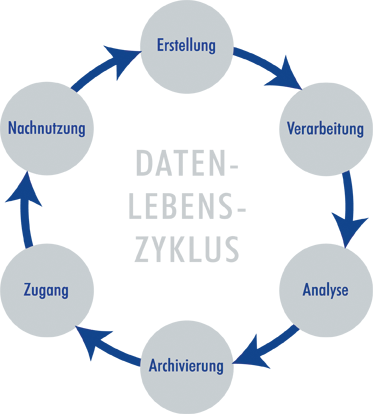
\includegraphics[width=0.51\textwidth]{bilder/Datenlebenszyklus}
  \end{center}
  \caption{Datenlebenszyklus}
\end{wrapfigure}

In der gegenwärtigen Praxis ist der Datenlebenszyklus oft unterbrochen, da nur einige wenige Daten ihren Weg in eine Publikation finden. Die übrigen Daten geraten auf den lokalen Speichermedien der Forscher in Vergessenheit oder werden komplett gelöscht und stehen somit einer Nachnutzung nicht mehr zur Verfügung. Diese Tatsache gilt es für die Zukunft zu verbessern und im Idealfall vollständig zu vermeiden.

Der hier vorgestellte Datenlebenszyklus beruht auf dem des "`UK Data Archive"'\footnote{\url{http://data-archive.ac.uk/create-manage/life-cycle}}. Er beschreibt sehr vereinfacht und idealtypisch die Abfolge der einzelnen Phasen im Zyklus aus einem eher praktischen Umgang mit Forschungsdaten. Es gibt auch andere komplexere Modelle, die einen anderen Blickwinkel beschreiben, wie etwa das "`Curation Lifecycle Model"'\footnote{\url{http://www.dcc.ac.uk/resources/curation-lifecycle-model}}, das verschiedene Tätigkeitsfelder bei der Erhaltung und Pflege der Daten beschreibt, und das "`Data Curation Continuum"'\footnote{\url{http://www.dlib.org/dlib/september07/treloar/09treloar.html}}, das vor allem auf die technischen Bedingungen eingeht und Daten unter dem Gesichtspunkt der Nutzergruppen, von privat bis öffentlich, beschreibt.

In jeder Phase des Datenlebenszyklus gelten unterschiedliche Schwerpunkte mit ihren eigenen Implikationen, die im Folgenden umrissen werden. In dem Kapitel Projektphasen ab Seite \pageref{projektphasen} werden die wichtigsten Aspekte dann ausführlich behandelt.

\subparagraph{Erstellung} Vor der eigentlichen Erstellung von neuen Daten muss schon die Projektplanung erfolgt und die Fragestellung formuliert sein, die maßgeblich bestimmen, wie die gesammelten und erzeugten Daten letztendlich aussehen sollen. Ein Bestandteil der Planung muss auch das Datenmanagement sein, das ab Seite \pageref{datenmanagement} beschrieben wird, um vorab festzulegen, welche Formate und Benennungsregeln verwendet werden sollen, wie die Speicherung und Sicherung der Daten und die Vernetzung von Daten und Projektmitarbeitern untereinander aussehen soll. Bereits vorhandene relevante Daten sollten lokalisiert und berücksichtigt werden. 

Schon während der Erstellung der Forschungsdaten erfolgt idealerweise die Beschreibung der Daten, da diese besonders im Hinblick auf die spätere Nachnutzung für die Verständlichkeit eine elementare Rolle spielt. Beispielsweise müssen die technischen Parameter der verwendeten Aufnahmegeräte so früh wie möglich dokumentiert werden.

\subparagraph{Verarbeitung} Sobald die Daten erhoben wurden, können sie verarbeitet werden. Dazu gehören verschiedene Abläufe, wie etwa Digitalisierung, Übersetzung, Überprüfung, Validierung, Bereinigung und andere Verarbeitungsformen mittels Programmen. Für einige Anwendungen oder im Hinblick auf eine spätere Veröffentlichung, kann eine Anonymisierung notwendig sein. Auch gilt es festzuhalten, wie Ausgangsdaten verändert und bearbeitet wurden. 

Außerdem ist die Beschreibung von Forschungsdaten ein wichtiger Aspekt für die Archivierung, um die Verständlichkeit für die spätere Nachnutzung deutlich zu erhöhen. Während der Verarbeitung von Forschungsdaten spielt die Verwaltung und Speicherung der Daten eine große Rolle, da gewährleistet werden muss, dass mit der richtigen Version gearbeitet wird und notfalls auch Sicherheitskopien zur Verfügung stehen.

\subparagraph{Analyse} Durch die Analyse und Interpretation der Forschungsdaten werden die Forschungsergebnisse gewonnen, die dann in Publikationen veröffentlicht werden. In der Regel sind die den neuen Erkenntnissen zugrunde liegenden Daten aber nur ein kleiner Bestandteil einer solchen Publikation. Jedoch werden alle Daten benötigt, um die Analyseergebnisse vollständig nachvollziehen zu können.

\subparagraph{Archivierung} Die Archivierung von Forschungsdaten beinhaltet die Auswahl und Umwandlung der einzelnen Dateien in geeignete Formate und deren Speicherung auf einem für die Archivierung geeigneten Medium. Die Erstellung und Speicherung von Backups gehört ebenfalls dazu.

Eine wesentliche Rolle bei der Archivierung spielt sowohl die strukturierte als auch die freie Beschreibung der Forschungsdaten, da diese Informationen darüber enthalten, wie und durch wen die Daten gewonnen wurden, welche Geräte dabei Verwendung fanden, wie diese konfiguriert waren und was die Daten bedeuten. 

\subparagraph{Zugang} Da das Ziel einer Datenarchivierung immer die Nachnutzbarkeit von Inhalten ist, sollten archivierte Daten im Rahmen rechtlicher Rahmenbedingungen verbreitet und Dritten ein Zugriff auf diese gewährt werden. Den Zugriff auf die Daten kann man mit verschiedenen Zugriffsrechten steuern, die es beispielsweise nur einer eingeschränkten Gruppe von Nutzern erlauben auf die Daten zuzugreifen. Bevor die Daten zugänglich gemacht werden, sollte man dafür sorgen, dass das Urheberrecht geklärt und gekennzeichnet ist.

Durch die Zugriffsgewährung wird die Sichtbarkeit von eigenen Forschungsleistungen erhöht.

\subparagraph{Nachnutzung} Archivierte Daten, die zugänglich gemacht wurden, können für eigene Forschungsvorhaben kostenlos wiederverwendet und neuen Analysen unterzogen werden. Durch die Nachnutzung wird die Nachprüfbarkeit von Ergebnissen im Sinne der guten wissenschaftlichen Praxis erleichtert.
%
%\chapter{Projektphasen}
%\chapter{Projektphasen}
	\abschnittsautor{S. Jahn, F. Schäfer, M. Trognitz}
	\label{projektphasen}

Im Umgang mit digitalen Daten gelten für jede Phase eines Forschungsprojektes unterschiedliche Anforderungen und Bedingungen. Da Forschungsdaten einem Lebenszyklus (siehe Seite \pageref{lebenszyklus}) unterliegen, haben Entscheidungen und Arbeitsschritte, die in einer bestimmten Phase getroffen werden, auch Auswirkungen auf die anderen Phase des Datenkreislaufs. Bereits bei Entwurf und Planung eines neuen Forschungsprojektes muss überlegt werden, welche Informationen bereits digital existieren, welche Arten von Dateien neu erzeugt werden müssen, welche Informationstechnologien zum Einsatz kommen sollen und wie das Management der Forschungsdaten gestaltet sein wird. 

Insofern gilt es einige Aspekte so früh wie möglich, häufig noch vor der Erstellung der ersten Datei, zu adressieren:
\begin{itemize}
\item Informationen über existierende Standards und Richtlinien einholen
\item Entscheidungen über die zu verwendenden Dateiformate und Softwareprogramme fällen
\item Verantwortliche für das Datenmanagement bestimmen
\item Kriterien für die laufende Dokumentation entwickeln
\item Konventionen für die Ablage, Benennung und Versionierung von Dateien festlegen
\item Strategien zur Speicherung und Sicherung definieren
\item Geeignete Infrastrukturen für die Archivierung auswählen und kontaktieren
\end{itemize}

Diese und weitere Fragen zur Vorbereitung, Durchführung und Nachbereitung eines Projektes werden im Folgenden anhand eines sogenannten Datenmanagementplans thematisiert. Der Datenmanagementplan bildet einen wichtigen Baustein zur Festlegung der Arbeitsabläufe im Umgang mit Forschungsdaten und für eine Kostenkalkulation.

Je mehr und je früher in den Einzelentscheidungen die Nachnutzung der Daten durch Dritte auch über die Lebensdauer eines Projektes hinaus berücksichtigt wird und die Langzeitarchivierung als kontinuierliche Maßnahme und nicht als letzter Schritt eines bereits abgeschlossenen Projektes begriffen wird, umso leichter gelingt es, einmal erhobene Daten auch für die Zukunft zu erhalten. Die Archivierung der Daten nach Abschluss eines Projektes wird erleichtert, wenn schon während der Durchführung eines Projektes auf die konsequente Erfüllung der im Datenmanagementplan genannten Aufgaben geachtet wird.

Das Finanzierungskonzept eines Forschungsprojektes sollte neben Hard- und Softwareausstattung ausdrücklich angemessene Anteile für Personalkosten und Dienstleistungen berücksichtigen. Im Zweifelsfall ist es ratsam, sich hierbei beraten zu lassen. Ab einer bestimmten Projektgröße bzw. Umfang der zu prozessierenden Daten sollten eine oder mehrere Personalstellen eingeplant werden, die überwiegend oder ausschließlich für IT-Belange zuständig sind. 

Vor oder kurz nach Beginn des Projektes erstellte und kommunizierte Richtlinien, ermöglichen es allen Projektmitarbeitern diese auch einzuhalten. Auf diese Weise wird die Handhabung der Projektdaten erheblich erleichtert, da geregelte Ordnerstrukturen und vorgegebene Namenskonventionen das Auffinden der Daten vereinfachen, die parallele Dokumentation das Verstehen und die Nachnutzung ermöglicht und Sicherungskopien das Risiko eines Datenverlustes reduzieren.

Abweichungen von den hier aufgeführten Empfehlungen sind nicht auszuschließen, doch sollten diese bewusst diskutiert und in Abwägung der jeweiligen Vor- und Nachteile entschieden werden.

\newpage
\section{Datenmanagement}\label{datenmanagement}
\abschnittsautor{M. Trognitz, D. Hagmann, J. Räther, S. Jahn}
Bereits vor Beginn eines Forschungsvorhabens steht die Konzeption und Planung des Projektes. Dazu gehört auch eine Beschreibung über den Umgang mit den resultierenden Forschungsdaten, der sogenannte Datenmanagementplan. Ein vollständiger Datenmanagementplan berücksichtigt alle Phasen des auf Seite \pageref{lebenszyklus} beschriebenen Lebenszyklus von Forschungsdaten. Er dient zunächst als Mittel zur strukturierten Reflexion über datenrelevante Aspekte eines Projektes und beantwortet grundsätzliche Fragen zu Verantwortlichkeiten, Maßnahmen zur Pflege und Verarbeitung der Daten, Standards und bereits vorhandenen Daten. Außerdem bietet er die Grundlage für Arbeitsabläufe (Workflows) im Umgang mit Forschungsdaten und für eine Kostenkalkulation.

Eine vollständige Dokumentation des Datenmanagements in einem Datenmanagementplan spart Zeit und Kosten, wenn beispielsweise Zusammenhänge beim Wechsel von Mitarbeitern hergestellt werden sollen, und beugt einem Datenverlust vor. Da die Nachnutzung von Forschungsdaten zunehmend an Bedeutung gewinnt, setzen Geldgeber oft einen Datenmanagementplan als Teil eines Förderantrags voraus.

Die konsequente Einhaltung aller im Datenmanagementplan gemachten Vorgaben während der gesamten Projektlaufzeit stellt sicher, dass die Daten auch von Dritten interpretiert und nachgenutzt werden können. Wird das Überführen der Daten in ein Archiv schon von Beginn des Projektes an vorbereitet und einkalkuliert ist zum Projektabschluss nur noch ein geringer Aufwand für die Übergabe in ein Archiv erforderlich, weil die Umformatierung, Neustrukturierung oder nachträgliche Dokumentation von Daten wegfällt.

Ein aktives Datenmanagement beugt insbesondere während der Planung und Durchführung eines Projektes späteren Zeit- und Budgetverlusten vor und stellt sicher, dass Daten am Ende in nachhaltigen Formaten, gut dokumentiert und gut strukturiert vorliegen.
% implementing data management measures during the planning and development stages of research will avoid later panic and frustration

\subsection{Übersicht der Aufgaben in den Projektphasen}
Mit Hilfe des zu Beginn eines Projektes erstellten Datenmanagementplans können sämtliche Prozesse während des Projekts strategisch umgesetzt werden, wobei die Umsetzung des Plans als laufender Vorgang zu verstehen ist. Wenn während eines Projektes Änderungen an dem Datenmanagementplan notwendig werden, sollten diese begründet, dokumentiert sowie Arbeitsprozesse und Ergebnisse angepasst werden. Außerdem muss dokumentiert werden wie die Änderungen sich auf bereits bestehende Daten auswirken.

In den unterschiedlichen Phasen des Datenlebenszyklus und des Projektes sind die Aspekte des Datenmanagementplans unterschiedlich stark zu berücksichtigen. Die folgende Tabelle veranschaulicht, wann im Lebenszyklus von Forschungsdaten welchen Aufgaben aus dem Datenmanagement besondere Aufmerksamkeit zuteil werden muss.

In Abhängigkeit der Projektgröße kann der Umfang der Aufgaben des Datenmanagementplanes und der Plan selbst skaliert werden, wobei jedoch Minimalanforderungen einzuhalten sind, um zuallererst die Verfügbarkeit der Daten im laufenden Projekt zu gewährleisten. Um die Planungen zu erleichtern und zu beschleunigen,  sollten bereits vorhandene institutionelle Vorgaben und Infrastrukturen genutzt werden.

\begin{table}[hbt]
\begin{tabular}{r!\tbg c!\tbg c!\tbg c!\tbg c!\tbg c!\tbg c!\tbg c!\tbg}
	\arrayrulecolor{ianusGrau}
 	\multicolumn{1}{r}{} & \multicolumn{1}{c}{\rot{Vorbereitung}} & \multicolumn{1}{c}{\rot{Erstellung}}& \multicolumn{1}{c}{\rot{Verarbeitung}} & \multicolumn{1}{c}{\rot{Analyse}} & \multicolumn{1}{c}{\rot{Archivierung}} & \multicolumn{1}{c}{\rot{Zugang}} & \multicolumn{1}{c}{\rot{Nachnutzung}}\\
	\cline{2-8}
	Rahmendaten\tib{*} & $\tib{\CIRCLE}$ & $\tib{\Circle}$ & $\tib{\Circle}$ & $\tib{\Circle}$ & $\tib{\RIGHTcircle}$ & $\tib{\Circle}$ & $\tib{\Circle}$\\
	\cline{2-8}
	Verantwortlichkeiten\tib{*} & $\tib{\CIRCLE}$ & $\tib{\Circle}$ & $\tib{\Circle}$ & $\tib{\Circle}$ & $\tib{\Circle}$ & $\tib{\Circle}$ & $\tib{\Circle}$\\
	\cline{2-8}
	Rechtliche Aspekte\tib{*} & $\tib{\CIRCLE}$ & $\tib{\Circle}$ & $\tib{\Circle}$ & $\tib{\Circle}$ & $\tib{\CIRCLE}$ & $\tib{\CIRCLE}$ & $\tib{\CIRCLE}$\\
	\cline{2-8}
	Methoden & $\tib{\CIRCLE}$ & $\tib{\CIRCLE}$ & $\tib{\RIGHTcircle}$ & $\tib{\RIGHTcircle}$ & $\tib{\Circle}$ & $\tib{\Circle}$ & $\tib{\Circle}$\\
	\cline{2-8}
	Vorgaben und Standards\tib{*} & $\tib{\CIRCLE}$ & $\tib{\CIRCLE}$ & $\tib{\CIRCLE}$ & $\tib{\Circle}$ & $\tib{\CIRCLE}$ & $\tib{\RIGHTcircle}$ & $\tib{\Circle}$\\
	\cline{2-8}	
	Kosten \& Ressourcen\tib{*} & $\tib{\CIRCLE}$ & $\tib{\CIRCLE}$ & $\tib{\CIRCLE}$ & $\tib{\Circle}$ & $\tib{\RIGHTcircle}$ & $\tib{\Circle}$ & $\tib{\Circle}$\\
	\cline{2-8}
	Externe Partner & $\tib{\CIRCLE}$ & $\tib{\CIRCLE}$ & $\tib{\RIGHTcircle}$ & $\tib{\Circle}$ & $\tib{\Circle}$ & $\tib{\RIGHTcircle}$ & $\tib{\CIRCLE}$\\
	\cline{2-8}
	Hard- und Software\tib{*} & $\tib{\CIRCLE}$ & $\tib{\CIRCLE}$ & $\tib{\RIGHTcircle}$ & $\tib{\RIGHTcircle}$ & $\tib{\Circle}$ & $\tib{\Circle}$ & $\tib{\Circle}$\\
	\cline{2-8}
	Datentypen und Datenformate & $\tib{\RIGHTcircle}$ & $\tib{\CIRCLE}$ & $\tib{\CIRCLE}$ & $\tib{\Circle}$ & $\tib{\CIRCLE}$ & $\tib{\Circle}$ & $\tib{\Circle}$\\
	\cline{2-8}
	Nachnutzung vorhandener Daten\tib{*} & $\tib{\RIGHTcircle}$ & $\tib{\RIGHTcircle}$ & $\tib{\CIRCLE}$ & $\tib{\CIRCLE}$ & $\tib{\Circle}$ & $\tib{\RIGHTcircle}$ & $\tib{\Circle}$\\
	\cline{2-8}
	Datenerzeugung \& -prozessierung\tib{*} & $\tib{\RIGHTcircle}$ & $\tib{\CIRCLE}$ & $\tib{\RIGHTcircle}$ & $\tib{\Circle}$ & $\tib{\RIGHTcircle}$ & $\tib{\RIGHTcircle}$ & $\tib{\Circle}$\\
	\cline{2-8}
	Datenmenge & $\tib{\CIRCLE}$ & $\tib{\CIRCLE}$ & $\tib{\CIRCLE}$ & $\tib{\CIRCLE}$ & $\tib{\RIGHTcircle}$ & $\tib{\Circle}$ & $\tib{\Circle}$\\
	\cline{2-8}
	Dateispeicherung und -sicherung\tib{*} & $\tib{\RIGHTcircle}$ & $\tib{\CIRCLE}$ & $\tib{\CIRCLE}$ & $\tib{\CIRCLE}$ & $\tib{\Circle}$ & $\tib{\Circle}$ & $\tib{\Circle}$\\
	\cline{2-8}
	Dateiverwaltung & $\tib{\RIGHTcircle}$ & $\tib{\CIRCLE}$ & $\tib{\CIRCLE}$ & $\tib{\CIRCLE}$ & $\tib{\RIGHTcircle}$ & $\tib{\Circle}$ & $\tib{\Circle}$\\
	\cline{2-8}
	Dokumentation\tib{*} & $\tib{\RIGHTcircle}$ & $\tib{\CIRCLE}$ & $\tib{\CIRCLE}$ & $\tib{\CIRCLE}$ & $\tib{\CIRCLE}$ & $\tib{\RIGHTcircle}$ & $\tib{\Circle}$\\
	\cline{2-8}
	Qualitätssicherung & $\tib{\RIGHTcircle}$ & $\tib{\CIRCLE}$ & $\tib{\CIRCLE}$ & $\tib{\CIRCLE}$ & $\tib{\CIRCLE}$ & $\tib{\Circle}$ & $\tib{\CIRCLE}$\\
	\cline{2-8}
	Datenaustausch & $\tib{\RIGHTcircle}$ & $\tib{\RIGHTcircle}$ & $\tib{\CIRCLE}$ & $\tib{\CIRCLE}$ & $\tib{\Circle}$ & $\tib{\CIRCLE}$ & $\tib{\Circle}$\\
	\cline{2-8}
	Mittelfristige Datenaufbewahrung & $\tib{\RIGHTcircle}$ & $\tib{\CIRCLE}$ & $\tib{\CIRCLE}$ & $\tib{\CIRCLE}$ & $\tib{\Circle}$ & $\tib{\Circle}$ & $\tib{\Circle}$\\
	\cline{2-8}
	Langfristige Archivierung\tib{*} & $\tib{\RIGHTcircle}$ & $\tib{\RIGHTcircle}$ & $\tib{\RIGHTcircle}$ & $\tib{\RIGHTcircle}$ & $\tib{\CIRCLE}$ & $\tib{\Circle}$ & $\tib{\CIRCLE}$ \\
	\cline{2-8}
	Zugänglichkeit und Nachnutzung & $\tib{\CIRCLE}$ & $\tib{\RIGHTcircle}$ & $\tib{\RIGHTcircle}$ & $\tib{\RIGHTcircle}$ & $\tib{\CIRCLE}$ & $\tib{\CIRCLE}$ & $\tib{\CIRCLE}$\\
	\cline{2-8}
	Projektabschluss & $\tib{\RIGHTcircle}$ & $\tib{\Circle}$ & $\tib{\Circle}$ & $\tib{\Circle}$ & $\tib{\RIGHTcircle}$ & $\tib{\RIGHTcircle}$ & $\tib{\Circle}$\\
	\cline{2-8}
\end{tabular}
\caption{Tabellarische Übersicht über die verschiedenen zu berücksichtigenden Aspekte eines Datenmanagementplans während unterschiedlicher Projektphasen und unter Beachtung des Lebenszyklus von Forschungsdaten. Besonders wichtige, als Minimalanforderung zu betrachtende Aspekte des Datenmanagementplans sind mit einem Stern gekennzeichnet.}
\label{tab:dmp-lebenszyklus}
\end{table}
\begin{table}[h!bt]
\begin{tabular}{cr}
	$\tib{\CIRCLE}$ & Aufgabe ist während der Phase relevant.\\
	$\tib{\RIGHTcircle}$ & Aufgabe ist während der Phase teilweise relevant.\\
	$\tib{\Circle}$ & Aufgabe ist während der Phase nicht relevant.\\
\end{tabular}
\end{table}
\subsection{Datenmanagementplan}
Die einzelnen in einem Datenmanagementplan zu berücksichtigenden Aspekte werden im Folgenden kurz skizziert, wobei diese Liste keinen Anspruch auf Vollständigkeit erhebt, sondern vor allem als Anregung für verschiedene Themenfelder gedacht ist. Zu einigen Aspekten folgen ausführlichere Abschnitte im Anschluss an diese Übersicht. 

Die Aufgaben können grob in drei Phasen gegliedert werden:
\begin{itemize}
    \item Planungsphase (ab Seite \pageref{dmp-planung})
    \item Durchführungsphase (ab Seite \pageref{dmp-durchfuehrung})
    \item Abschlussphase (ab Seite \pageref{dmp-abschluss})
\end{itemize}

\label{dmp-planung}\paragraph{Planungsphase}
In der Planungsphase eines Projektes ist es im Hinblick auf den Datenmanagementplan insbesondere notwendig, die hierfür erforderlichen Ressourcen einzuplanen. Diese stehen in direkter Abhängigkeit von dem allgemeinen Rahmendaten und den anzuwendenden Methoden. Sie umfassen sowohl den technischen, als auch den personellen Aufwand. Neben der allgemeinen Festlegung von Verantwortlichkeiten empfiehlt es sich, für den Datenmanagementplan als ganzes oder spezifischer Teile und Datenarten Datenverantwortliche zu benennen.

\subparagraph{Rahmendaten und administrative Angaben}
\begin{itemize}
    \item Welche allgemeinen Informationen und Rahmenbedingungen des Projektvorhabens kontextualisieren das Vorhaben und die Daten? (z.B. Eckdaten des Projektes wie Titel, Namen der Verantwortlichen, Partner, Methoden und Laufzeit)
    \item Was sind, zusammengefasst, die Ziele und das Vorhaben?
    \item Wer sind die Projektträger und Finanzgeber?
\end{itemize}
Dazu kann auch die Liste für Projektbezogene Metadaten ab Seite \pageref{Metadaten-anwendung} konsultiert werden.

\subparagraph{Verantwortlichkeiten}
\begin{itemize}
    \item Wie werden die Rollen und Zuständigkeiten beim Datenmanagement eingeteilt?
    \item Wer beaufsichtigt die Einhaltung des Datenmanagementplans und der daraus resultierenden Vorgaben?
    \item Wer ist für Hard- und Software zuständig?
    \item Wer kümmert sich um die Sicherung der Daten und Backups?
    \item Wer sind institutionelle Ansprechpartner?
    \item Wer sind sonstige Ansprechpartner?
    \item Wer kümmert sich um die Integrität der Daten?
    \item Wie werden die Verantwortlichkeiten kommuniziert?
    \item Ist für eine Kontinuität bei den Verantwortlichkeiten gesorgt?
    \item Wer bekommt welche Berechtigungen für welche Daten?
    \item Gibt es für bestimmte Datenarten Datenverantwortliche?
\end{itemize}

\subparagraph{Rechtliche Aspekte}
\begin{itemize}
    \item Welche Daten sind urheberrechtlich geschützt?
    \item Welche Daten fallen unter Datenschutz?
    \item Wie werden die Rechte am geistigen Eigentum für die Daten von Beginn an dokumentiert?
    \item Gibt es Anforderungen und Einschränkungen für eine Veröffentlichung der Daten?
    \item Mit welchen Lizenzen sollen die Daten für Dritte zur Verfügung gestellt werden?
\end{itemize}

\subparagraph{Methoden}
\begin{itemize}
    \item Welche Methode oder Grabungsmethode wird angewandt?
    \item Hat die Fundstelle oder das Projektvorhaben Einfluss auf die zu verwendenden Methoden?
    \item Gibt es Richtlinien oder Best-Practices für die eingesetzten Methoden?
    \item Welche Dokumentationsmethoden kommen zum Einsatz?
    \item Beeinflusst die zu verwendende Methode die Datenmenge?
\end{itemize}

\subparagraph{Vorgaben, Richtlinien und Standards}
\begin{itemize}
    \item Gibt es Gesetze, Vorschriften der Institution, der Projektträger, der Geldgeber, der externen Partner, der zuständigen Landesämter, die eingehalten werden müssen?
    \item Kann eine bestehende institutionelle Infrastruktur zur Organisation, Verwaltung und Speicherung der Daten genutzt werden?
    \item Sind externe Standards und Richtlinien für den Umgang mit den Daten bekannt?
    \item Welche Qualitätsvorgaben sind für die verschiedenen Datenarten notwendig?
    \item Müssen eigene Vorgaben definiert werden?
    \item Gibt es Checklisten zur Kontrolle der Einhaltung von Vorgaben?
\end{itemize}

\subparagraph{Kosten und Ressourcen}
\begin{itemize}
    \item Wie hoch werden die anfallenden Kosten für Personal und Technik eingeschätzt?
    \item Berücksichtigt die Kostenkalkulation die Kosten in Abhängigkeit der zu erwartenden Datenmenge?
    \item Fallen weitere Kosten für externe Partner oder Dienstleister an?
    \item Muss mit zusätzlichen Kosten für spezielle Anwendungen, Werkzeuge, Systeme etc. gerechnet werden?
    \item Wie sind die Kosten für die Publikation der Ergebnisse zu erwarten?
    \item Welche Folgekosten sind nach Projektende zu erwarten, beispielsweise für die Archivierung der Forschungsdaten?
    \item Welche weiteren Ressourcen werden benötigt?
    \item Bei reproduzierbaren Daten: Sind die Kosten für eine Aufbewahrung höher als für eine Wiederbeschaffung?
    \item Welche Kosten fallen einmalig an, welche regelmäßig?
    \item Können Kosten durch regelmäßige Aufgaben oder durch eine frühzeitige Berücksichtigung von bestimmten Aufgaben verringert werden? (z.B. Dokumentation, Auswahl für das Archiv)
    \item Wer trägt welche Kosten?
    \item Kann der Standard während der gesamten Laufzeit gehalten werden?
\end{itemize}
Weitere Hinweise zur Planung von Kosten und Ressourcen sind in der Broschüre “Einstieg ins Forschungsdatenmanagement in den Geowissenschaften” des EWIG-Projektes ab Seite 11 zu finden. (http://doi.org/10.2312/lis.14.01)


\label{dmp-durchfuehrung}\paragraph{Durchführungsphase}
Während der Durchführung eines Projektes werden die in der Planungsphase gesammelten und erstellten Vorgaben umgesetzt und deren Einhaltung aktiv kontrolliert, sowie bei Bedarf angepasst. 

Eine zeitnah nach Plan durchgeführte Erstellung, Verarbeitung, Analyse und Dokumentation von Daten und Arbeitsabläufen vermeidet eine lange und kostenintensive Abschlussphase. 

\subparagraph{Externe Partner oder Dienstleister}
\begin{itemize}
    \item Mit welchen externen Partnern soll kooperiert werden?
    \item Welche Dienstleister sollen in Anspruch genommen werden?
    \item Welche Auflagen entstehen dadurch und sind diese mit den eigenen Vorgaben vereinbar?
    \item Wie erfolgt der Datenaustausch?
    \item Bei wem verbleiben die Rechte an den Daten?
    \item Wie werden die verschiedenen Vorgaben und Richtlinien an externe Partner kommuniziert?
\end{itemize}

\subparagraph{Hard- und Software}
\begin{itemize}
    \item Welche Hard- und Software steht zur Verfügung?
    \item Werden spezielle Geräte oder Programme benötigt?
    \item Erfüllen die Systeme die vorgegebenen Auflagen, etablierte Standards und die Anforderungen an ein nachhaltiges Datenmanagement?
    \item Können kostenpflichtige Programme durch frei verfügbare Programme (sogenannte Open-Source-Software) ersetzt werden?
\end{itemize}

\subparagraph{Datentypen und Datenformate}
\begin{itemize}
    \item Welche Daten werden verwendet oder erzeugt? (z.B. Beobachtungs- und Messdaten, prozessierte Daten etc.)
    \item In welchen Formaten werden die Daten erzeugt und in welchen sollen sie gesichert werden?
    \item Welches Dateiformat ist für die Archivierung geeignet?
    \item Gibt es verbreitete Standards, die bei der Wahl des Formats zu beachten sind?
    \item Können offene Formate verwendet werden oder müssen proprietäre verwendet werden und hat das Implikationen für die verwendete Hard- und Software?
\end{itemize}
Weitere Informationen sind in den Kapiteln "`Dateiformate"' ab Seite \pageref{dateiformate} und "`Forschungsmethoden"' ab Seite \pageref{methoden} zu finden.

\subparagraph{Nachnutzung vorhandener Daten}
\begin{itemize}
    \item Gibt es bereits vorhandene Daten, die nachgenutzt werden können?
    \item Wurde nach Datenbeständen im Besitz der eigenen Institution oder von Dritten recherchiert?
    \item Wie sind deren Zugriffsmöglichkeiten und Urheberrechte?
    \item Ist die Qualität der Daten ausreichend? (z.B. geeignete Formate, ausreichend Dokumentation)
    \item Wie wird die Integration zwischen bereits bestehenden und neuen Daten organisiert?
    \item Sind auch analoge Quellen zu berücksichtigen?
\end{itemize}

\subparagraph{Erzeugung und Prozessierung von Daten}
\begin{itemize}
    \item Welche Daten müssen neu erzeugt werden oder können bestehende nachgenutzt werden, um das Projektziel zu erreichen?
    \item Handelt es sich um einmalige Daten oder können sie reproduziert werden?
    \item Welche Rolle spielen die Daten innerhalb des Projektes? (z.B. Dokumentation, Publikation, Nachnutzung etc.)
    \item Gibt es sensible oder besonders schützenswerte Daten?
    \item Kann man Anforderungen potentieller Nachnutzer bei der Datenerzeugung mitberücksichtigen?
\end{itemize}

\subparagraph{Datenmenge}
\begin{itemize}
    \item Wie groß ist die zu erwartende Datenmenge für die Gesamtdauer des Projekts?
    \item Hat das Folgen für die Speicherung und Sicherung der Daten? (z.B. längere Backup-Zeiten)
    \item Ergeben sich daraus besondere Anforderungen an die technische Infrastruktur? (z.B. mehr Speicherplatz)
    \item Fallen verschiedene Bearbeitungsstufen mit verschiedenen Versionen an, die gegebenenfalls ein Versionierungssystem erfordern?
\end{itemize}
Weitere Informationen zur Versionierung sind in dem Abschnitt "`Versionskontrolle"' ab Seite \pageref{versionskontrolle} zu finden.

\subparagraph{Dateispeicherung und -sicherung}
\begin{itemize}
    \item Welche Maßnahmen zur Dateispeicherung und -sicherung sind während des Projekts notwendig?
    \item Auf welcher Hardware sollen die Daten gesichert werden? (z.B. Server oder Festplatten)
    \item Wie oft, womit und durch wen werden Backups durchgeführt?
    \item Wer ist für die Datenspeicherung und -sicherung verantwortlich?
    \item Gibt es ein Disaster Management?
    \item Wurden die Maßnahmen zur Dateiwiederherstellung geprobt?
\end{itemize}
Weitere Informationen sind im Abschnitt "`Dateispeicherung und -sicherung"' ab Seite \pageref{dateispeicherung} zu finden.

\subparagraph{Dateiverwaltung}
\begin{itemize}
    \item Wie sollen Dateien benannt, geordnet und versioniert werden?
    \item Gibt es Benennungsregeln für die Dateien?
    \item Kann auf auf bestehende Vorgaben und Systeme für die Dateiverwaltung zurückgegriffen werden?
    \item Sind Verzeichnisstrukturen logisch nachvollziehbar und selbsterklärend?
    \item Ist die Datenablage dokumentiert?
    \item Wie ist der Umgang mit verschiedenen Dateiversionen geplant?
    \item Ist der Einsatz eines Versionierungssystems notwendig?
    \item Werden Daten, die für eine künftige Nachnutzung geeignet sind oder archiviert werden sollen, gesondert verwaltet?
\end{itemize}
Weitere Informationen sind im Abschnitt "`Dateiverwaltung"' ab Seite \pageref{dateiverwaltung} zu finden.

\subparagraph{Dokumentation}
\begin{itemize}
    \item Wie sollen die Daten beschrieben werden, damit sie kurz- und langfristig lesbar und verständlich sind?
    \item Welche Informationen sind zur Dokumentation der Forschungsdaten notwendig?
    \item Zu welchem Zeitpunkt muss die Dokumentation geschehen?
    \item Gibt es Vorgaben oder Standards dafür?
    \item Werden Veränderungen und Aktualisierungen der Daten dokumentiert?
    \item Wie sollen Metadaten abgelegt und gespeichert werden?
    \item Werden Anpassungen an der Projektstruktur und dem Datenmanagementplan dokumentiert?
    \item Werden Ausnahmen dokumentiert?
    \item Gibt es Werkzeuge, die den Dokumentationsprozess unterstützen?
\end{itemize}
Weitere Informationen sind im Abschnitt "`Dokumentation"' ab Seite \pageref{Metadaten-allgemein} zu finden.

\subparagraph{Qualitätssicherung}
\begin{itemize}
    \item Welche Kriterien sind hinsichtlich vorhandener Standards zur Qualitätssicherung zu beachten?
    \item Wie werden Vorgaben zu Formaten und zur Datenbearbeitung eingehalten?
    \item Sind die Daten genau, konsistent und authentisch?
    \item Sind die Daten vollständig?
    \item Wie steht es um die Integrität der Daten?
    \item Sind die Daten verständlich Dokumentiert und geht aus der Dokumentation hervor: \emph{Wer} hat \emph{wann}, zu welchem \emph{Zweck}, \emph{was} und \emph{womit} gemacht?
    \item Wird eine Qualitätskontrolle durchgeführt?
    \item Gibt es Checklisten zur unterstützung der Qualitätskontrolle?
    \item Welche Maßnahmen gegen ein versehentliches Löschen oder eine Manipulation der Daten werden getroffen?
\end{itemize}

\subparagraph{Datenaustausch}
\begin{itemize}
    \item Wie ist der Datenaustausch zwischen den Projektbeteiligten geplant?
    \item Welche technische Infrastruktur ist für den Datenaustausch erforderlich?
    \item Sind gesetzliche Vorgaben oder andere Einschränkungen zu beachten?
    \item Wie soll auf die Daten zugegriffen werden?
    \item Welche Nutzungsrechte liegen für die Daten vor?
\end{itemize}


\label{dmp-abschluss}\paragraph{Abschlussphase}
In der das Projekt abschließenden Phase müssen besonders Entscheidungen sowohl zur mittelfristigen Datenaufbewahrung, als auch zur langfristigen Archivierung der im Projekt generierten Daten und Ergebnisse getroffen werden. Neben der Klärung der organisatorischen und rechtlichen Rahmenbedingungen muss hierbei spezielles Augenmerk auf die Regelung der Zugänglichkeit zu den langzeitarchivierten Daten und der Nachnutzung gelegt werden. So wird sichergestellt, dass über den Projektabschluss hinaus die Daten langfristig zur Verfügung stehen. 

\subparagraph{Mittelfristige Datenaufbewahrung}
\begin{itemize}
    \item Welche Gründe gibt es für eine Aufbewahrung der Daten?
    \item Liegen Vorgaben zur Aufbewahrungsdauer der Daten vor?
    \item Liegen Vorgaben zu Aufbewahrungsorten der Daten vor?
    \item Welche Daten sollen oder müssen aufbewahrt werden, welche Daten sollen oder können gelöscht werden?
    \item Sind sie selbst Hersteller der Daten?
    \item Ist die Aufbewahrung von Fremddaten zwingend notwendig?
    \item Wie lange sollen die Daten aufbewahrt werden?
    \item Wie und wo sollen die Daten aufbewahrt werden?
    \item Wer ist für die Aufbewahrung der Daten verantwortlich?
    \item Sind Kosten zu erwarten?
\end{itemize}

\subparagraph{Vorbereitung für die langfristige Archivierung}
\begin{itemize}
    \item Welche Daten sollen archiviert werden?
    \item Liegen Kriterien für die Auswahl der Daten vor?
    \item Gibt es eine passende Archivlösung?
    \item Wurde bereits Kontakt mit dem Archiv aufgenommen?
    \item Welche Besonderheiten gilt es zu beachten? (z.B. eine gesonderte Aufbereitung der Daten)
    \item Wann und durch wen werden die Daten übergeben?
\end{itemize}

\subparagraph{Zugänglichkeit und Nachnutzung}
\begin{itemize}
    \item Wie sollen die Daten zugänglich sein?
    \item Welche Zusatzinformationen sind für das Verständnis der Daten notwendig?
    \item Wer darf die Daten nutzen, welche Lizenzen sollen verwendet werden?
    \item Gibt es Einschränkungen für den Zugriff auf und die Nutzung der Daten?
    \item Auf welche Weise sollen die Daten zur Verfügung gestellt werden?
\end{itemize}

\subparagraph{Projektabschluss}
\begin{itemize}
    \item Liegt die Dokumentation vollständig und den Vorgaben entsprechend vor?
    \item Ist eine gesonderte abschließende Dokumentation erforderlich?
    \item Ist der Datenmanagementplan in die Dokumentation integriert?
    \item Ist die Nachnutzbarkeit der Forschungsdaten auch nach Projektende gewährleistet?
    \item Wie ist die mittelfristige Aufbewahrung der Daten geregelt?
    \item Wie ist die langfristige Archivierung der Daten geregelt?
    \item Wie ist die Zugänglichkeit der Daten geregelt?
\end{itemize}

%XXX Grafik zur Visualisierung vom DMP: Mit Waben oder Puzzleteilen

\subsection{Weiterführende Informationen}
\paragraph{Quellen}
\begin{flushleft}
Archaeology Data Service, Planning for the Creation of Digital Data \urllist{http://guides.archaeologydataservice.ac.uk/g2gp/CreateData_1-0}
Archaeology Data Service, Data Management and Sharing Plans \urllist{http://archaeologydataservice.ac.uk/advice/DataManagementPlans}
Archaeology Data Service, DataTrain. Open Access Post-Graduate Teaching Materials in Managing Research Data in Archaeology \urllist{http://archaeologydataservice.ac.uk/learning/DataTrain}
S. Büttner --  H.-C. Hobohm -- L. Müller (Hrsg.) Handbuch Forschungsdatenmanagement (Bad Honnef 2011)\abstand
DCC (Hrsg.) Data Management Plans \urllist{http://www.dcc.ac.uk/resources/data-management-plans}
Helmholtz-Zentrum Potsdam - Deutsches GeoForschungsZentrum GFZ -- Bibliothek und Informationsdienste -- Institut für Meteorologie der FU Berlin -- Konrad-Zuse-Zentrum für Informationstechnik Berlin (Hrsg.) Einstieg ins Forschungsdatenmanagement in den Geowissenschaften (2014), DOI: 10.2312/lis.14.01 \urllist{http://doi.org/10.2312/lis.14.01}
HU Berlin (Hrsg.)  Datenmanagementplan. Anleitung zur Erstellung eines Datenmanagementplans (DMP) \urllist{https://www.cms.hu-berlin.de/de/dl/dataman/arbeiten/dmp_erstellen}
U. Jakobsson, Data Management Planning. What it is and how to do it (2013) \urllist{http://www.ariadne-infrastructure.eu/fre/Events/ARIADNE-Workshop-EAA-2013/Agenda-Presentations/DataManagementPlanning_SND_Ujakobsson_04092013}
H. Neuroth -- A. Oßwald -- R. Scheffel -- S. Strathmann -- M. Jehn (Hrsg.) nestor Handbuch. Eine kleine Enzyklopädie der digitalen Langzeitarchivierung. Version 2.0 (2009) Kap.3:15 \abstand
K. Perrin -- D. H. Brown -- G. Lange -- D. Bibby -- A. Carlsson -- A. Degraeve -- M. Kuna -- Y. Larsson -- S. U. Pálsdóttir -- B. Stoll-Tucker -- C. Dunning -- A. Rogalla von Bieberstein, A Standard and Guide to Best Practice for Archaeological Archiving in Europe, EAC Guidelines 1 (2013) \urllist{http://archaeologydataservice.ac.uk/arches/Wiki.jsp?page=The\%20Standard\%20and\%20Guide\%20to\%20Best\%20Practice\%20in\%20Archaeological\%20Archiving\%20in\%20Europe}
UK Data Archive (Hrsg.) Create \& Manage Data. Planning for Sharing \urllist{http://data-archive.ac.uk/create-manage/planning-for-sharing}
Uni Marburg (Hrsg.) Projekt "Kompetenzzentrum Forschungsdatenmanagement und -archivierung" \urllist{https://www.uni-marburg.de/projekte/forschungsdaten}
V. van den Eynden -- L. Corti -- M. Woollard -- L. Bishop -- L. Horton, Managing and Sharing Data. Best Practice for Researchers (Essex 2011) \urllist{http://ukdataservice.ac.uk/manage-data/handbook.aspx}
WissGrid (Hrsg.) Leitfaden Forschungsdaten-Management (2011) \urllist{http://www.wissgrid.de/publikationen/deliverables/wp3/WissGrid-oeffentlicher-Entwurf-Leitfaden-Forschungsdaten-Management.pdf}

\quelltyp{Beispiele für Datenmanagementpläne}
DataONE (Hrsg.) Data Management Planning \urllist{https://www.dataone.org/data-management-planning}
DCC (Hrsg.) Data plan guidance and examples \urllist{http://www.dcc.ac.uk/resources/data-management-plans/guidance-examples}
MITLibraries (Hrsg.) Write a Data Management Plan \urllist{http://libraries.mit.edu/data-management/plan/write/\#Resources}

\quelltyp{Checklisten und Tools für Datenmanagementpläne}
DCC (Hrsg.) Checklist for a Data Management Plan (2014) \urllist{http://www.dcc.ac.uk/webfm_send/1279}
DCC (Hrsg.) DMPOnline \urllist{https://dmponline.dcc.ac.uk/}
J. Richards, Online Resources for Data Management Planning (2013) \urllist{http://www.ariadne-infrastructure.eu/fre/Events/ARIADNE-Workshop-EAA-2013/Agenda-Presentations/DataManagementPlanning_Online_Resources_ADS_JRichards_04092013}
RDMO (Hrsg.) Research Data Management Organiser \urllist{http://rdmorganiser.github.io/software/}
WissGrid (Hrsg.) Checkliste zum Forschungsdaten-Management (2011) \urllist{http://www.wissgrid.de/publikationen/deliverables/wp3/WissGrid-oeffentlicher-Entwurf-Checkliste-Forschungsdaten-Management.pdf}
\end{flushleft}

\newpage
\section{Dokumentation}\label{Metadaten-allgemein}
\abschnittsautor{D. Bibby, P. Gerth, M. Heinrich, S. Jahn, B. Ludwig, A. Posluschny, E. Siegloff, A. Sieverling, M. Trognitz}
\hyphenation{
}

Das wichtigste Kriterium für die Archivierung und Nachnutzbarkeit von Daten ist neben technischen Aspekten, wie die Wahl eines geeigneten Langzeitformates, eine vollständige Dokumentation . Viele Dokumente und Dateien sind nicht aus sich selbst heraus verständlich. Sie stehen immer in einem gewissen Forschungs- oder Projektkontext, der für die Nachnutzung dokumentiert werden muss. Damit Forschungsdaten von Dritten gefunden und sinnvoll verwertet werden können, müssen sie durch zusätzliche Informationen ergänzt und strukturiert beschrieben werden. Wenn Daten ausreichend fachlich wie technisch beschrieben werden, können sie durch andere Personen wissenschaftlich nachgenutzt werden und besitzen somit einen Wert für die Zukunft. Nur dann lohnt sich auch der Aufwand einer analogen oder digitalen Langzeitarchivierung.

Die Dokumentation eines Projektes und der erzeugten Daten sollte als ein wichtiger, kontinuierlicher Prozess verstanden werden, der von Anfang an berücksichtigt und während des gesamten Lebenszyklus von Daten umgesetzt wird -- und nicht erst nach Abschluss von Arbeiten oder bei der Übergabe von Beständen an ein Archiv. Insofern bedarf es innerhalb von größeren Projekten eines Verantwortlichen oder einer Organisationsform aller Beteiligten, welche die Struktur und Pflege der Dokumentation konzeptionell und koordinierend begleitet. Gemeinsam muss definiert werden, welcher Gegenstand dokumentiert wird, in welchem Umfang und mit welcher Gliederung, welche Form geeignet ist (z. B. Wiki versus PDF), wie die Aktualität der Inhalte erhalten wird, wie Nutzer über Änderungen informiert werden usw. Fehlende Strategien für den Aufbau und die Pflege einer Dokumentation führen häufig zu Unübersichtlichkeit und dadurch zu einer Konfusion der beteiligten Akteure. Von umfassenden, detaillierten und strukturierten Angaben zu  digitalen Daten profitieren nicht nur die Archive und zukünftige Generationen von Forschern, sondern auch die Wissenschaftler selbst während der Durchführung eines Projektes -- genauso wie es auch bei einer guten analogen Dokumentenablage der Fall ist.

Welche Informationen sind für eine Dokumentation erforderlich? Wichtig sind alle Angaben, die den Entstehungsprozess und -kontext sowie die Konventionen von Inhalten und Daten beschreiben oder zumindest skizzieren. Dabei kann die Dokumentation als "`Beipackzettel"' verstanden werden, der anderen Personen das Auffinden der Daten, das Verstehen der Inhalte, eine sinnvolle Wiederverwendung der Daten für weitere Forschungen ermöglicht und die Vergleichbarkeit von Daten erhöht. So ist es beispielsweise üblich, bei Fotografien das Aufnahmedatum, eine Kurzbeschreibung des abgelichteten Gegenstandes und den Fotografen anzugeben, Zeichnungen mit einem Maßstab, der geografischen Ausrichtung, dem Zeichner und einem Kurztext zu beschriften oder bei Texten einen Autor, einen Titel und ein Datum zu nennen.

Insbesondere bei digitalen Daten sind zusätzliche, spezialisierte Informationen erforderlich, die über die rein deskriptiven Angaben zu den Inhalten und zum Forschungsinteresse hinausgehen und nicht nur die primären Fragen zu \emph{"`Wer, Wie, Was, Wo, Wann und Warum?"'} beantworten. So sind technische und administrative Angaben über die Vorgehensweise der Datenerhebung und die eingesetzten Programme, mit denen die Daten erzeugt oder digitalisiert wurden, für ein späteres Auslesen, Auswerten und Interpretieren unverzichtbar. Auch wie die Daten strukturiert wurden und in welcher Beziehung Dateien zueinander stehen, muss in der Regel explizit erklärt werden. Angaben zu Qualitätssicherungsverfahren,  Änderungshistorie und Versionierung von Daten erlauben es, das empirische Vorgehen im Forschungsprozess nachzuprüfen. Zudem ist es wichtig zu erklären, wie Dritte zukünftig auf die Daten zugreifen  oder sie nutzen dürfen.

Damit unbeteiligte Personen den größeren Zusammenhang einer einzelnen Information oder eines Datenbestandes verstehen und nachvollziehen können, sollte jede Dokumentation eines Projektes mindestens folgende Punkte enthalten:
\begin{itemize}
	\item Angaben zur Fragestellung und zum Untersuchungsgegenstand
	\item Angaben zu den Projektverantwortlichen für Nachfragen
	\item Zusammenfassung der wissenschaftlichen Ergebnisse
	\item Beschreibung von Arbeitsabläufen und Methoden, vor allem bezüglich der Datenerhebung, -verarbeitung und Qualitätssicherung
	\item Auflistung der erzeugten unterschiedlichen Dokumentarten (z. B. Tagebücher, Berichte, Listen, Fotos etc.)
	\item Beschreibung von verwendeten Handbüchern, Standards, projektspezifischen Konventionen, Thesauri, Nummernsystemen etc.
	\item Auflistung der eingesetzten technischen Geräte und Programme
	\item Relevante Publikationen und wichtige Sekundärliteratur
	\item Wichtige Korrespondenzen, Verträge, Anträge etc. (ggf. in anonymisierter Form) 
	\item Bestimmungen zur weiteren freien oder eingeschränkten Verwendung von Daten
\end{itemize}

In dem Abschnitt Speicherung von Metadaten ab Seite \pageref{metadatenSpeicherung} sind weitere allgemeine Angaben zu finden. In dem Kapitel Dateiformate ab Seite \pageref{dateiformate} werden außerdem weitere notwendige Angaben abhängig vom Dateityp aufgelistet. Auch für die Anwendung von bestimmten Methoden werden gesonderte Dokumentationsangaben erforderlich, die in dem Kapitel Forschungsmethoden ab Seite \pageref{methoden} zu finden sind.


%##################################################################################

\subsection{Dokumentation mit Metadaten}
Ein spezifischer Bestandteil einer jeden Dokumentation sind Metadaten. Während die Dokumentation die Summe aller Angaben zu einem Projekt und der zugehörigen Daten umfasst und sie in Form, Inhalt, Länge und Struktur je nach fachlichen Gepflogenheiten völlig frei formuliert sein kann, sind Metadaten nach festen formalen Kriterien strukturiert (z. B. als Formulare oder Eingabemasken) und beschreiben die Eigenschaften von anderen Daten, ohne diese selbst zu enthalten.

Metadaten machen die fachlich oder organisatorisch notwendigen Kontextinformationen explizit und dienen zur Auffindung von relevanten Informationen, deren Identifikation, deren Auswahl und Verwaltung. Beispielsweise sind Fotos nur anhand der mit ihnen assoziierten beschreibenden Metadaten effizient durchsuch- und auffindbar oder Karten nur dank einer Maßstabsangabe und einer aussagekräftigen Legende wissenschaftlich nutzbar. Die National Information Standards Organization (NISO) definiert Metadaten als Werkzeuge, um Forschungsdaten nachhaltig zu organisieren, zu erschließen, zu verstehen und zu benutzen. Werden Metadaten standardisiert gespeichert, können sie auch maschinell verarbeitet werden.

Da Metadaten immer von unterschiedlichen Informationsbedürfnissen und Anwendungskontexten abhängig sind, lassen sie sich unter verschiedenen Blickwinkeln betrachten. Egal ob sie ein Forschungsvorhaben in seiner Gesamtheit oder den Inhalt eines einzelnen Dokuments beschreiben, können sie sich auf folgende Aspekte beziehen:
\begin{itemize}
	\item Deskriptive Angaben, die ein Projekt, ein Objekt oder eine Methode fachlich und inhaltlich näher beschreiben (z. B. Kurzbeschreibung eines Fotos, Laufzeit eines Forschungsvorhabens, Autor eines Textes)
	\item Strukturelle Angaben, welche die physischen oder logischen Beziehungen zwischen komplexen Objekten beschreiben (z. B. referenzierte Dateien in Zeichnungen, die Reihenfolge von Fotos oder zusammengehörige Dateien)
	\item Administrativ-rechtliche Angaben, die Rechteinhaber, Lizenzbedingungen und Zugangsregeln benennen und für die Verwaltung relevant sind (z. B. Fristen für die Veröffentlichung von Ergebnissen)
	\item Administrativ-erhaltungsbezogene Angaben, welche die Geschichte eines digitalen Objektes, also die  vorhergehenden und gegenwärtigen Zustände, nachvollziehen lassen und Erhaltungsmaßnahmen beschreiben (z. B. Angabe zur Herkunft einer Karte, Konvertierungsmaßnahmen)
	\item Technische Angaben, die Informationen zu Software und Hardware liefern (z. B. das Dateiformat eines Bildes, die Zeichenkodierung eines Textes oder technische Parameter eines Messgerätes). Sie werden benötigt, um Daten in veralteten Dateiformaten in neuere umwandeln oder um die ursprüngliche Programmumgebung mittels aktueller Technik nachbauen zu können.
\end{itemize}

Ein anderes Unterscheidungskriterium von Metadaten ist der Umfang der Daten, die sie beschreiben. Sie können sich beziehen auf:
\begin{itemize}
	\item Eine größere zusammenhängende Datensammlung (z. B. der gesamte Datenbestand eines Projektes)
	\item Eine einzelne Datei
	\item Eine einzelne Information innerhalb eines Systems (z. B. ein Datensatz in einer Datenbank)
\end{itemize}

Weiterhin können Metadaten auch angewandte Prozesse und Methoden beschreiben, um den Entstehungsprozess von Dateien und Dateikonvoluten verständlicher zu machen und Hinweise für den weiteren Umgang mit den Daten zu liefern. Im Abschnitt Metadaten in der Anwendung ab Seite \pageref{Metadaten-anwendung} werden daher Metadaten in drei Kategorien unterschieden:
\begin{itemize}
	\item Projektbezogene Metadaten, die den gesamten Datenbestand eines Projektes dokumentieren
	\item Dateibezogene Metadaten, die einzelne Dateien dokumentieren
	\item Methodenbezogene Metadaten, die angewandte Prozesse und Methoden dokumentieren
\end{itemize}

Außerdem kann bei Metadaten unterschieden werden zwischen solchen, die eine manuelle Eingabe erfordern, und solchen, die durch Systeme und Programme automatisch erzeugt werden können. Erstere können beispielsweise eine Kurzbeschreibung oder Schlagworte sein. Letztere sind Angaben wie Erstellungsdatum, Dateiname oder Einstellungen der Digitalkamera.

Während für ein laufendes Projekt nur ein Ausschnitt dieser Metadaten eine praktische Relevanz besitzt, sind für die digitale Langzeitarchivierung von Daten alle Aspekte wichtig. Einige der Metadaten können ausschließlich von beteiligten Personen frühzeitig während des Prozesses der Datenerzeugung erfasst werden, da nur sie den Inhalt, den Charakter, die Struktur, den Kontext und die Quellen der Daten kennen. Andere Metadaten dagegen lassen sich auch zu einem späteren Zeitpunkt bei der Archivierung und Veröffentlichung der Daten generieren.


%##################################################################################

\subsection{Strukturierung von Metadaten}
Die Struktur und der Umfang von Metadaten sind wesentliche Faktoren, um diese sinnvoll nutzen zu können. Die Art und Weise, wie die verschiedenen Informationen erfasst und organisiert werden, spielen dabei eine zentrale Rolle, ob sie von einer unbeteiligten dritten Person richtig verstanden werden und ob die Angaben automatisiert verarbeitet werden können. 

Um die Struktur und den Umfang von Metadaten verbindlich zu beschreiben und vorzugeben, werden Metadatenschemata verwendet. Ein Metadatenschema gibt den Inhalt und die Gliederung von Metadaten vor, also die zu verwendenden Metadaten-Kategorien. Beispielsweise kann eine Publikation mit den Attributen Autor -- Jahr -- Titel -- Reihe -- Verlag -- Erscheinungsort und Schlagworte beschrieben werden, die dann mit den entsprechenden Informationen gefüllt werden. Diese Minimalbeschreibung kann je nach Anforderungen erweitert werden, etwa um die Elemente Sprache -- Seitenzahl -- Abbildungszahl -- Auflage und ISBN-Nummer.

In einem Metadatenschema wird zudem für einzelne Informationen die Genauigkeit (die Granularität) der erwarteten Information festgelegt, also ob beispielsweise für das Attribut "`Autor"' eine freie Texteingabe ausreichend ist oder ob eine Aufteilung in die Teilattribute Anrede -- Titel -- Vorname(n) und Nachname sowie eine Referenz zu einer Personennormdatei erforderlich ist.

Für den Austausch von Metadaten zwischen verschiedenen technischen Systemen besitzen die zugrunde liegenden Schemata eine zentrale Bedeutung. Sollen Informationen aus unterschiedlichen Quellen miteinander in Beziehung gesetzt werden, so dass sie gemeinsam ausgewertet werden können, müssen die jeweils eingetragenen Werte auf der Ebene ihrer semantischen Bedeutung miteinander verknüpft und abgeglichen werden. Das heißt, dass neben dem eigentlichen Wert (z. B. die Zeichenkette "`Pompeji"') auch das Attribut angegeben werden muss, also die Eigenschaft, die durch den Wert beschrieben wird (z. B. "`Fundort"', "`Aufbewahrungsort"' oder "`Publikationsort"'). 

Für viele Bereiche, wie etwa Medienarchive, Bibliotheken oder Museen, gibt es langjährige Erfahrungen im Umgang mit Metadaten und es wurden spezifische Metadatenschemata entwickelt. Zu Beginn eines Projektes sollte geprüft werden, ob relevante Metadatenschemata bereits existieren oder sogar vorgegeben werden und bei der Erzeugung von eigenen Metadaten berücksichtigt werden sollten. Je internationaler und standardisierter ein verwendetes Schema ist, desto eher ist die Austauschbarkeit von Metadaten mit anderen Systemen gewährleistet. Sofern sich unterschiedliche Metadaten auf ein gemeinsames Metadatenschema abbilden (\emph{mappen}) lassen, können sie in ein drittes System importiert und dort gemeinsam geöffnet werden.

\begin{wrapfigure}{r}{0.5\textwidth}
  \begin{center}
    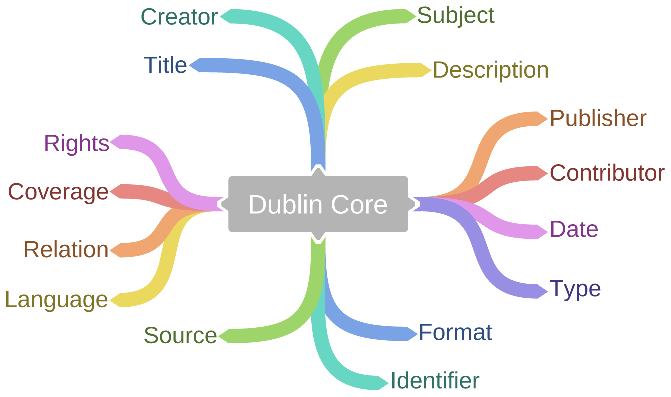
\includegraphics[width=0.5\textwidth]{bilder/doku_dublinCore}
  \end{center}
  \caption{Die 15 Kernfelder von Dublin Core Version 1.1. (Grafik erstellt mit coggle.it.)}
  \label{doku_dublinCore}
\end{wrapfigure}
Für deskriptive Metadaten ist das unter ISO 15836 zertifizierte Metadatenschema \emph{Dublin Core} (in Abbildung \ref{doku_dublinCore}) am weitesten verbreitet. Es verfügt in der Version 1.1 über folgende 15 Kernfelder: \emph{Title} (Titel) -- \emph{Creator} (Ersteller) -- \emph{Subject} (Thema) -- \emph{Description} (Beschreibung) -- \emph{Publisher} (Verleger) -- \emph{Contributor} (Mitwirkender) -- \emph{Date} (Datum) -- \emph{Type} (Typ) -- \emph{Format} (Format) -- \emph{Identifier} (Identifikator) -- \emph{Source} (Quelle) -- \emph{Language} (Sprache) -- \emph{Relation} (Beziehung) -- \emph{Coverage} (Umfang) -- \emph{Rights} (Rechte).

Im Laufe der Jahre wurde dieses grundlegende Set noch erweitert. Das aktuelle Set, "`\emph{The Dublin Core Metadata Initiative (DCMI) Metadata Terms}"', und die Beschreibung der einzelnen Attribute kann \href{http://dublincore.org/documents/dcmi-terms/}{online}\footnote{\href{http://dublincore.org/documents/dcmi-terms/}{http://dublincore.org/documents/dcmi-terms/}} abgerufen werden.

Eine besondere Relevanz im archäologischen und altertumswissenschaftlichen Kontext haben folgende Standards erlangt:
\begin{itemize}
	\item Online AccesS to the Index of archaeological investigationS (OASIS), veröffentlicht von English Heritage. Es wurde für den Nachweis von archäologischen Projekten und Maßnahmen in Großbritannien entwickelt. Das Schema liegt aktuell in Version 1.3 vor. Neben den in der Abbildung \ref{abb:doku_oasisProject} dargestellten fünf Themenbereichen können auch weitere spezielle Angaben wie etwa zu Arealen, Geophysik, Geologie und Artefakten gemacht werden.
	\begin{figure}[h!bt]
		\begin{center}
			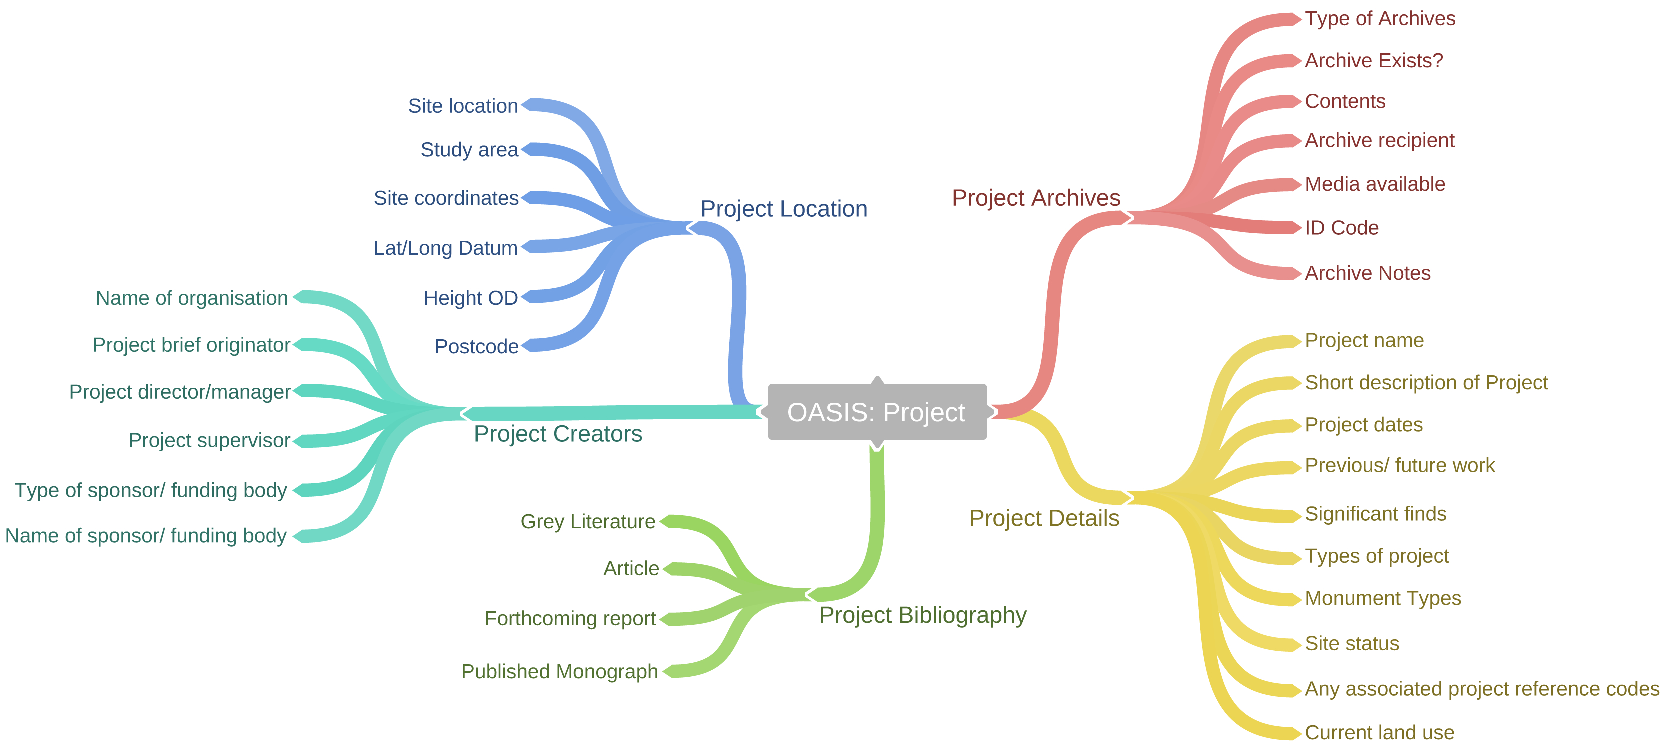
\includegraphics[width=\textwidth]{bilder/doku_oasisProject}
		\end{center}
		\caption{OASIS in Version 1.3. Neben den abgebildeten Themenbereichen sind auch Attribute für weitere spezialisiertere Informationen vorgesehen. (Grafik erstellt mit coggle.it.)}
		\label{abb:doku_oasisProject}
\end{figure}
	\item Archäologischer DateneXport-Standard (ADeX), wurde von der "`Kommission Archäologie und Informationssyteme"' beim Verband der Landesarchäologen entwickelt. Der Standard wurde für den Austausch archäologischer Fachdaten zwischen Landesämtern und anderen Institutionen erarbeitet. Die aktuelle in Abbildung \ref{abb:doku_ADeX} dargestellte Version ist 2.0, die auch den Austausch von komplexen Geometrien mittels externer Geometriedaten (SHP oder MIF) ermöglicht. ADeX ist bewusst als einfaches Austauschformat mit den Teilen "`Generelles"', "`Georeferenz"' und  "`Typ und Zeit"' unter Berücksichtigung internationaler Standards, wie etwa CIDOC-CRM, gestaltet. Dies gewährleistet eine hohe Austauschbarkeit.
	\begin{figure}[h!bt]
		\begin{center}
			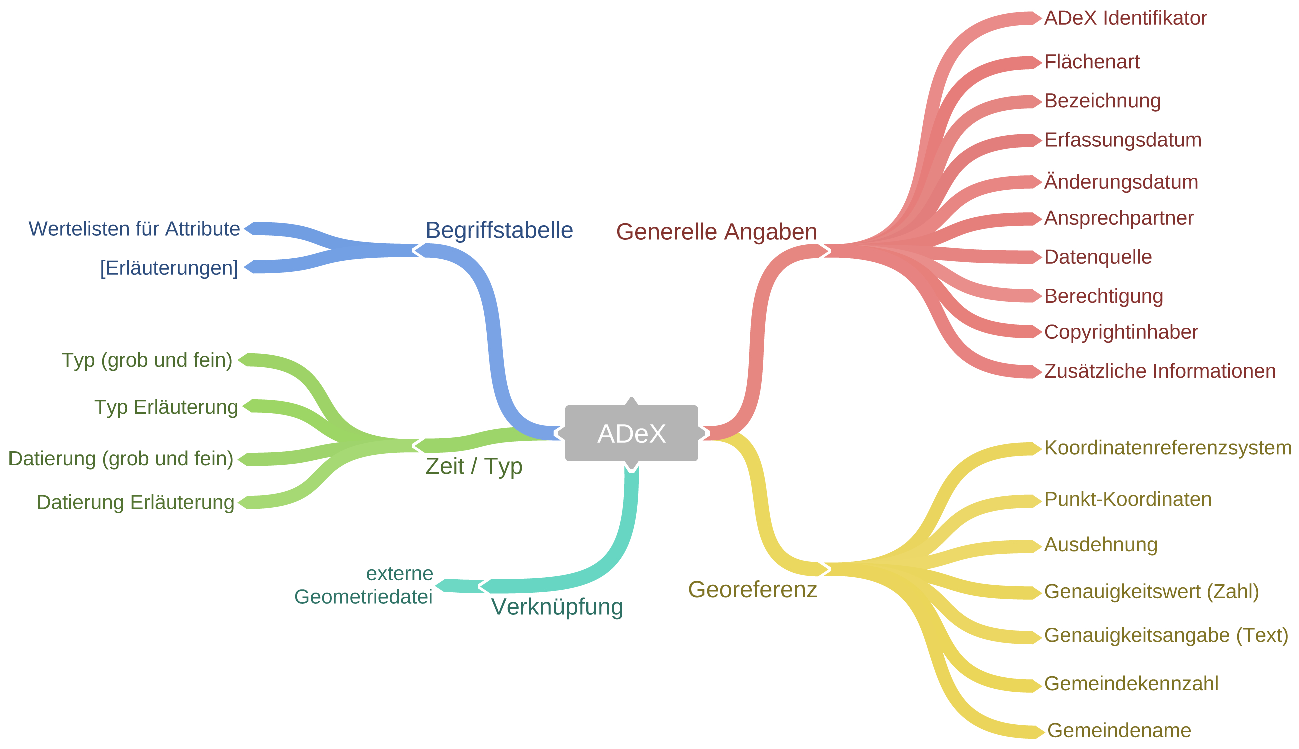
\includegraphics[width=\textwidth]{bilder/doku_ADeX}
		\end{center}
		\caption{ADeX in Version 2.0, das für eine hohe Kompatibilität auf detailliete Informationen verzichtet. (Grafik erstellt mit coggle.it.)}
		\label{abb:doku_ADeX}
\end{figure}
	\item Connecting Archaeology and Architecture in Europeana (CARARE) in Version 2.0. Es wurde als archäologiespezifisches Datenmodell unter Berücksichtigung verschiedener europäischer Standards von Europeana und dem Project 3D-ICONS entwickelt. Die Abbildung \ref{abb:doku_CARARE} verdeutlicht, dass in dem Schema Informationen zur Sammlung (\emph{Collection information}), zum physischen Objekt (\emph{Heritage asset}), zur digitalen Ressource (\emph{Digital resource}) und zur Aktivität (\emph{Activity}) definiert werden.
	\begin{figure}[h!tb]
		\begin{center}
			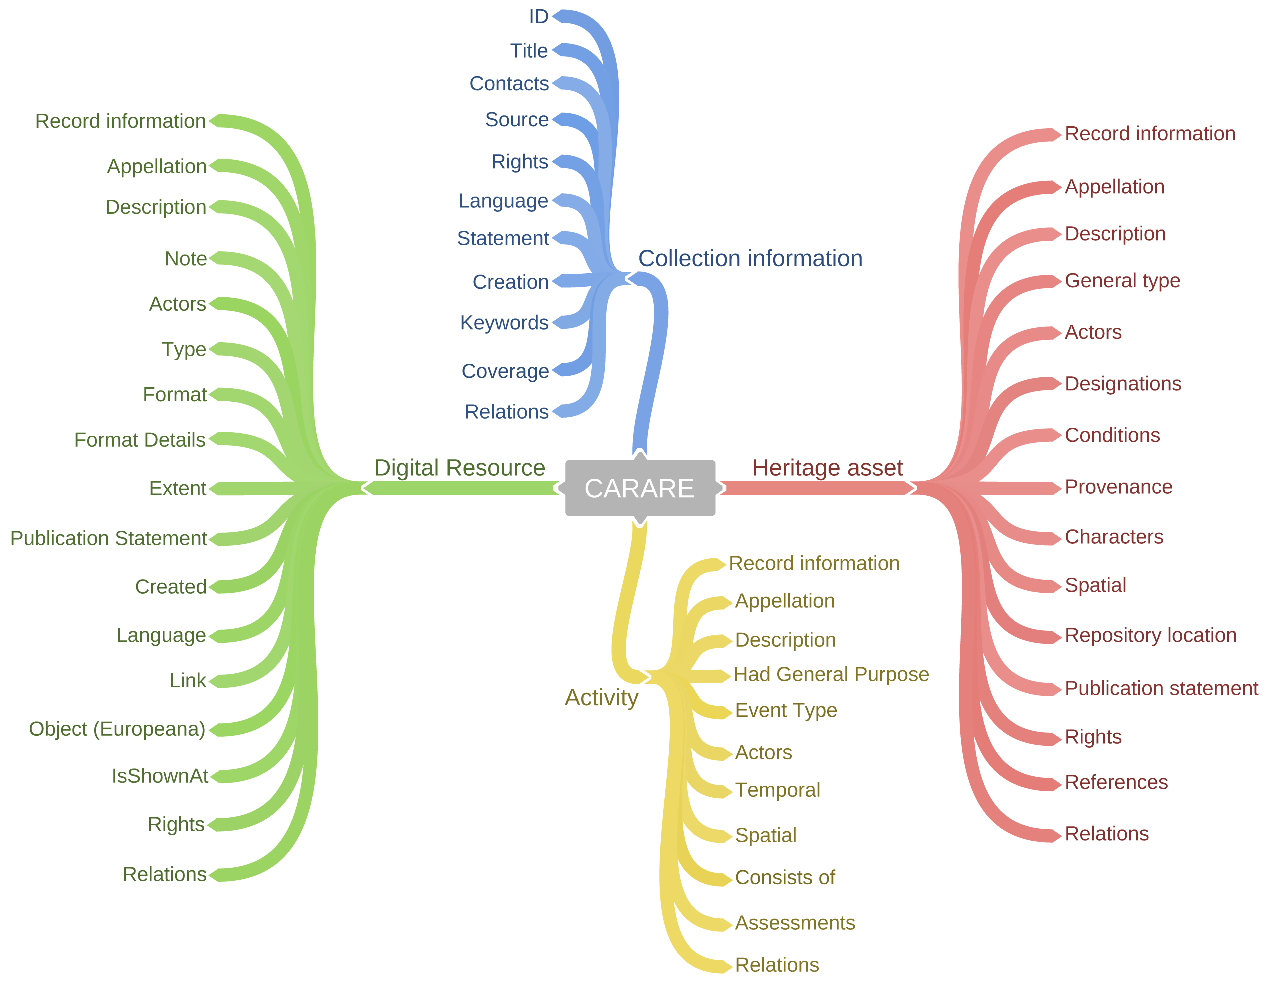
\includegraphics[width=0.9\textwidth]{bilder/doku_CARARE}
		\end{center}
		\caption{CARARE 2.0. (Grafik erstellt mit coggle.it.)}
		\label{abb:doku_CARARE}
\end{figure}
\item Das Metadatenschema von IANUS in Abbildung \ref{abb:doku_IANUS} wurde ebenfalls für Daten aus dem Bereich der Archäologien und Altertumswissenschaften entwickelt und orientiert sich an bereits vorhandenen Standards.
\begin{figure}[h!bt]
		\begin{center}
			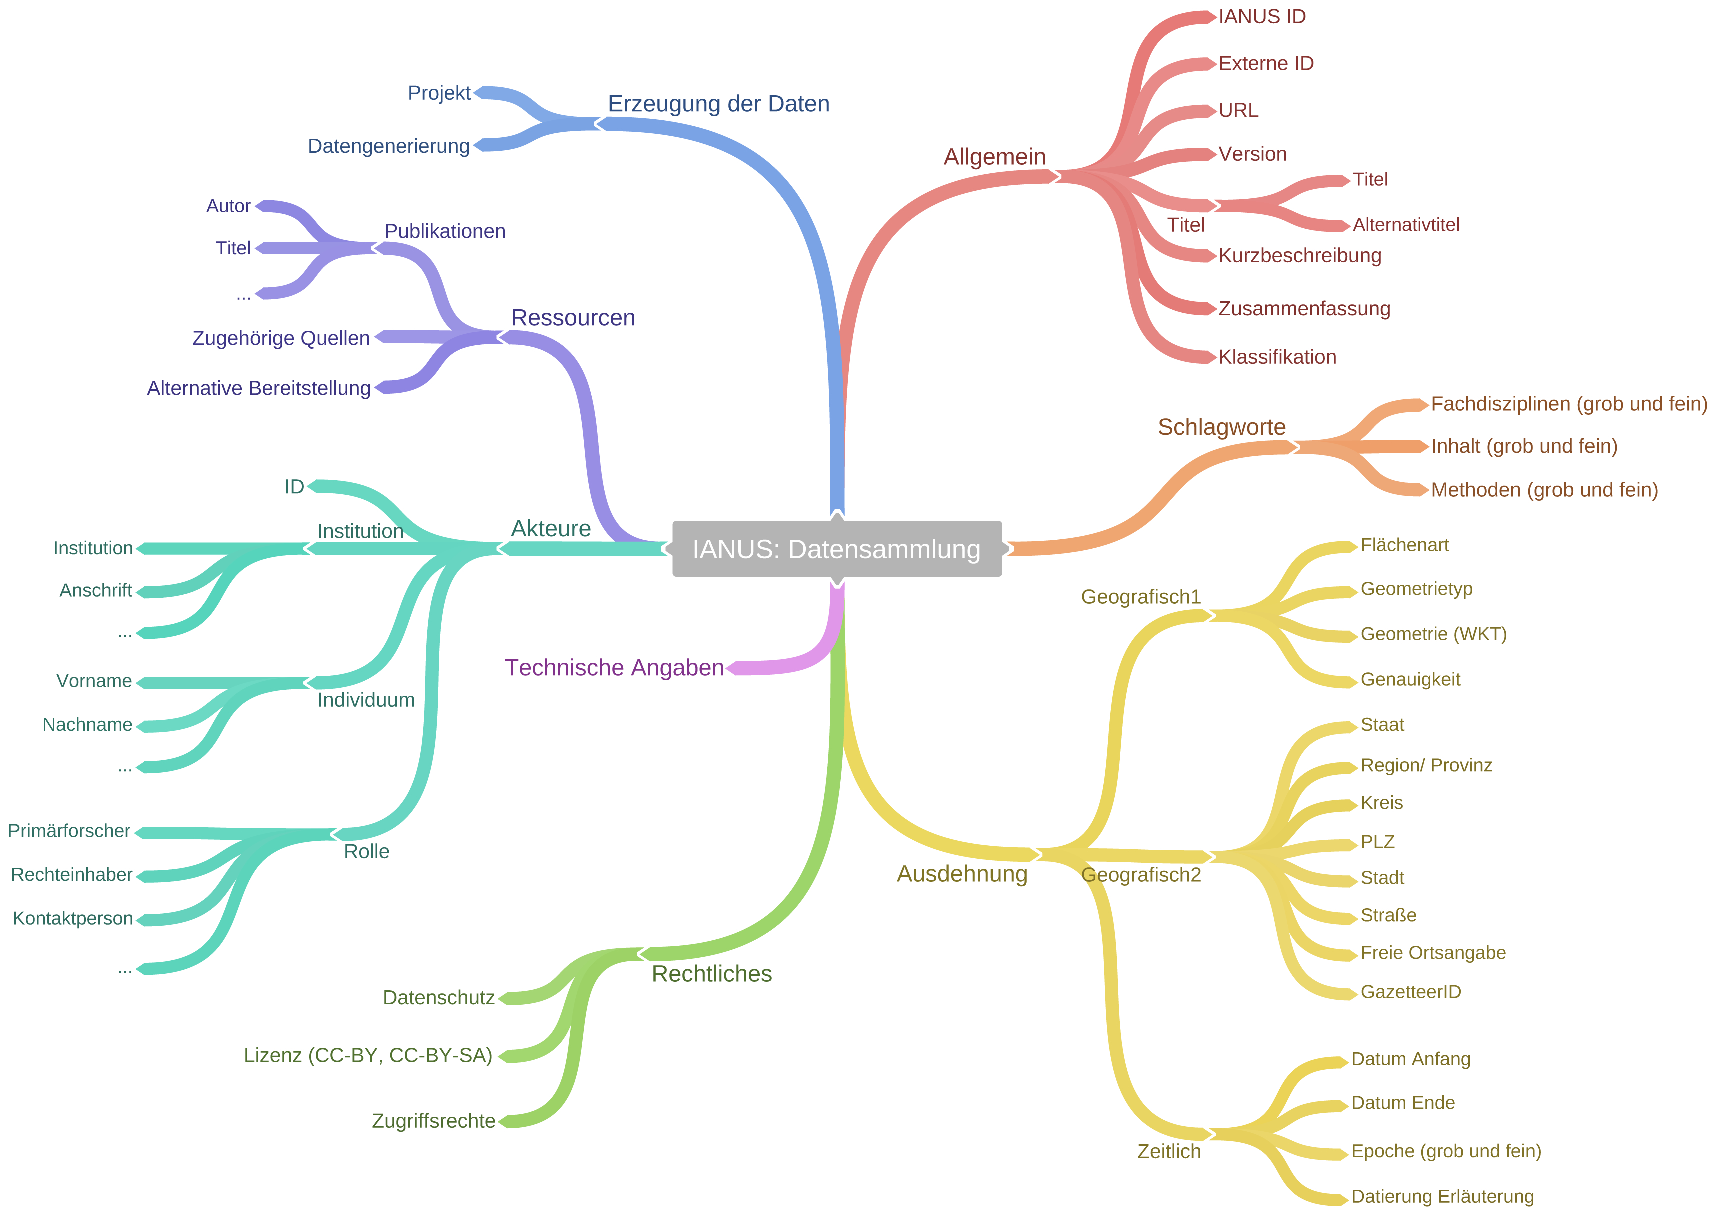
\includegraphics[width=\textwidth]{bilder/doku_IANUS}
		\end{center}
		\caption{Eine vereinfachte Darstellung des Metadatenschemas von IANUS. (Grafik erstellt mit coggle.it.)}
		\label{abb:doku_IANUS}
\end{figure}
\end{itemize}

Darüberhinaus gibt es weitere internationale Standards und institutionelle Vorgaben:
\begin{itemize}
	\item CIDOC Conceptual Reference Modell (CIDOC CRM) wurde von der Arbeitsgruppe "`Dokumentationsstandards"' im Internationalen Komitee für Dokumentation (CIDOC) des internationalen Museumsverbandes (ICOM) erarbeitet. Es dient der Strukturierung und formalen Beschreibung von Informationen, Konzepten und Relationen im Bereich des Kulturerbes. Seit 2006 ist CIDOC CRM unter ISO 21127 standardisiert. Für CIDOC-CRM gibt es zusätzlich die im Rahmen von ARIADNE entwickelten Erweiterungen CRMarchaeo, CRMba, CRNdig und CRMgeo, die eine Relevanz für die Archäologie haben. Sie werden in dem Ariadne Reference Model zusammengefasst.
	\item Das Lightweight Information Describing Objects (LIDO) wurde als Austauschformat für bewegliche Objekte in Museen von Arbeitsgruppen innerhalb von CIDOC entwickelt.
	\item Historic Environment Records oder MIDAS Heritage aus Großbritannien.
	\item Vorgaben verschiedener Denkmalämter. Weitere Informationen dazu sind in dem Abschnitt "`Grabungsdokumentation"' ab Seite \pageref{grabungsdokumentation} zu finden.
\end{itemize}


%##################################################################################

\subsection{Kontrollierte Vokabulare, Thesauri und Normdaten}
Damit Metadaten möglichst sinnvoll genutzt und maschinell verarbeitet werden können, sollten neben klar definierten Metadatenschemata auch möglichst einheitliche Begriffe und homogene Beschreibungen verwendet werden. Nur wenn gleiche Dinge auch mit den gleichen Begriffen benannt werden, ist es möglich vollständige und präzise Suchergebnisse zu erhalten oder vergleichbare Daten richtig miteinander zu verknüpfen. Die Vorgabe und Definition von festen Begriffen und Regeln hilft zudem, Mehrdeutigkeiten und Redundanzen zu vermeiden, etwa wenn eine Zeichenkette verschiedene Bedeutungen besitzen kann (z. B. Abakus als Rechenhilfsmittel oder als architektonischer Abschluss eines Kapitells), ein identischer Sachverhalt durch unterschiedliche Worte erfasst werden kann (z. B. Survey und Oberflächenbegehung) oder die Form der Angabe variieren kann (z. B. ein Datum in der Form 12.03.2012 oder 2012-03-12).
 
Das geeignete Mittel zur Vereinheitlichung der sprachlichen Vielfalt sind sogenannte kontrollierte oder normierte Vokabulare, die entweder einfache Wortlisten oder strukturierte Thesauri sein können, in denen Wörter zusammen mit ihrem semantischen Kontext verwaltet werden. Diese "`terminologische Kontrolle"' kann in unterschiedlicher Weise systematisiert und implementiert sein. 

Beispielsweise können innerhalb eines Projektes alle zu verwendenden Begriffe unter allen Beteiligten abgestimmt, klar fachlich definiert, voneinander abgegrenzt und in strukturierter Form dokumentiert werden. Diese Absprachen können dann in einem zentralen Textdokument als Projektleitfaden abgelegt oder in einer Datenbank als Felder umgesetzt werden, die nur eine begrenze Auswahl von Begriffen zur Beschreibung eines spezifischen Sachverhaltes zulassen (z. B. für das Attribut Filmart nur die Werte "`Diapositiv (Farbe)"', "`Negativfilm (Farbe)"', "`Negativfilm (SW)"' und "`Digital"').

Besser eignen sich jedoch etablierte, standardisierte, globale Vokabulare, Thesauri oder Normdateien. Sie weisen oft eine thematische, fachspezifische oder institutionelle Ausprägung auf und werden von maßgeblichen Einrichtungen kontinuierlich gepflegt. Dazu gehören beispielsweise Normdateien zur Katalogisierung aus dem Bibliotheksbereich, Personennormdateien oder Thesauri zur eindeutigen Identifizierung von geografischen Orten oder Zeitbegriffen. 

Diese globalen Systeme bieten nicht nur eine feste Bezeichnung und eine Definition eines Begriffes oder des diesem zugrunde liegenden Konzeptes, sondern auch alternative und gegebenenfalls mehrsprachige Benennungen und eine eindeutige Kennung zur Identifizierung des Begriffes. So kann beispielsweise der Ort "`Alexandria"' (\href{http://www.geonames.org/361058/alexandria.html}{361058}) in Ägypten von dem Ort "`Alexandria"' (\href{http://www.geonames.org/4744091/alexandria.html}{4744091}) in den USA mittels der in den Klammern angegebenen Kennungen aus GeoNames unterschieden werden.

Bereits existierende Thesauri und Vokabulare sollten bei der Vergabe von Metadaten berücksichtigt und angewendet werden, um den späteren elektronischen Austausch, also die Interoperabilität, der eigenen Daten mit anderen Systemen erheblich zu vereinfachen. Wenn Ressourcen in mehreren Sprachen vorliegen und entsprechend multilingual beschrieben werden sollen, müssen die genutzten Wörterbücher, Thesauri und Schlagwortsysteme äquivalente Begriffe in mehreren Sprachen abbilden.

Für die systematische Erfassung archäologischer und allgemeiner Begriffe existieren folgende Vokabulare:
\begin{itemize}
	\item Art \& Architecture Thesaurus (AAT) wurde Ende der 1970er von dem Getty Research Institute entwickelt, um die Katalogisierungsprozesse in Kunstbibliotheken und im Museumsbereich zu unterstützen und zu vereinheitlichen. Dieser Thesaurus wird von einer breiten Fachgemeinschaft kuratiert.
	\item Heritage Data -- Linked Data Vocabularies for Cultural Heritage führt die in England genutzten Vokabulare im Bereich kulturelles Erbe zusammen. 
	\item Wortnetz Kultur (WNK) wurde vom Landschaftsverband Rheinland ins Leben gerufen, um die Inhalte in deren verschiedenen Informationssystemen zu vereinheitlichen. Mittlerweile sind die Themen Kulturlandschaft, Archäologie, Kulturanthropologie, Denkmalpflege sowie Kunstgeschichte mit rund 15.000 Begriffen vertreten.
	\item Das DAI bietet mit iDAI.vocab (auch archwort) ein flaches multilinguales Vokabular mit Links auf den AAT. Außerdem gibt es mit dem iDAI.the"-sau"-rus ein System, das die Schlagworte aus den unterschiedlichen Thesauri der Bibliotheken zusammenführt und strukturiert.
	\item Die Encyclopedia of Life stellt eine weltweite Datenbank für Pflanzen und Lebewesen dar, die zusätzlich Fotos, Verbreitungskarten und Literaturhinweise enthält.
	\item In Wikidata werden alle strukturierten Daten aus den Systemen von WikiMedia erfasst und mit eindeutigen Identifikatoren zur Verfügung gestellt.
\end{itemize}

Für die eindeutige Identifizierung von geografischen Orten eignen sich, neben den amtlichen Gemeindekennzahlen und dem geodätischen Parameterdatensatz EPSG, folgende Ortsthesauri, sogenannte Gazetteers:
\begin{itemize}
	\item GeoNames ist ein Gazetteer, in dem vor allem moderne Orte, deren alternative Bezeichnungen und geografischen Koordinaten systematisch erfasst werden. Die Inhalte stammen von engagierten Nutzern weltweit.
	\item Getty Thesaurus of Geographic Names (TGN) wurde 1987 von dem Getty Research Institute ins Leben gerufen, um ebenfalls deren Katalogisierungsprozesse in Kunstbibliotheken und im Museumsbereich zu unterstützen und zu vereinheitlichen.
	\item Das DAI betreibt mit dem iDAI.gazetteer einen Gazetteer für die eindeutige Adressierung von antiken Orten, in dem außerdem auch die Eintragungen in GeoNames berücksichtigt werden.
	\item Pleiades ist ebenfalls ein Gazetteer für antike Orte mit einem Schwerpunkt auf der griechischen und römischen Antike, dessen Inhalt durch jeden Nutzer erweitert oder korrigiert werden kann.
\end{itemize}

Auch für Zeitbegriffe gibt es kontrollierte Vokabulare:
\begin{itemize}
	\item PeriodO ist ein Gazetteer für Zeitepochen. Neben der zeitlichen Information wird auch die geografische Verbreitung der jeweiligen Epoche erfasst.
	\item iDAI.chronontology ist ein vom DAI durchgeführtes Projekt, das wie PeriodO zeitliche und geografische Informationen miteinander in Beziehung setzt.
\end{itemize}

Zur Erfassung von Informationen zu Personen oder Institutionen sollten Normdateien verwendet werden, wie beispielsweise:
\begin{itemize}
	\item Das Virtual International Authority File (VIAF) kombiniert Normdateien mehrerer Nationalbibliotheken und speichert Informationen zu Personen und Institutionen, sowie deren Publikationen.
	\item Die Open Researcher and Contributor ID (ORCID) ist eine alphanumerische Zeichenkette, die der eindeutigen Identifizierung wissenschaftlicher Autoren dient. ORCID wird von einem gemeinnützigen Gremium betrieben und Autoren müssen sich selbst registrieren, um eine ID zu bekommen.
	\item Die Gemeinsame Normdatei (GND) der Deutschen Nationalbibliothek dient primär der Katalogisierung in Bibliotheken. Neben Informationen zu Personen und Körperschaften werden auch weitere Informationen zu Konferenzen, Geografika, Sachschlagwörtern und Werktiteln verwaltet.
\end{itemize}

Wenn in Metadaten auf Publikationen verwiesen werden soll, eignen sich folgende Systeme:
\begin{itemize}
	\item Die Internationale Standardbuchnummer (engl. \emph{International Standard Book Number}, ISBN) wird zur eindeutigen Identifizierung von Publikationen verwendet. Sie ist vor allem im Buchhandel verbreitet. Für Reihen und Zeitschriften wird eine ähnliche Nummer, die ISSN (Internationale Standardnummer für fortlaufende Sammelwerke, engl. \emph{International Standard Serial Number}) verwendet.
	\item Für in Deutschland veröffentlichte Medienwerke gibt es eine Ablieferungspflicht bei der Deutschen Nationalbibliothek, weshalb die dort vergebenen  eindeutigen Kennungen ebenfalls zur Identifizierung verwendet werden können.
	\item Für archäologische und altertumswissenschaftliche Publikationen eignen sich auch die Identifikatoren aus iDAI.bibliography (Zenon), in dem die umfangreichen Bestände aller DAI Bibliotheken nachgewiesen werden.
\end{itemize}

%##################################################################################
\label{metadatenSpeicherung}
\subsection{Speicherung von Metadaten}
Für eine strukturierte Speicherung von Metadaten gibt es verschiedene Möglichkeiten und Wege, die einerseits von dem Zeitpunkt (synchron mit der Datenerhebung oder im Nachhinein) und andererseits von der Art der Metadatenerfassung (manuell oder automatisiert) abhängen. 

Grundsätzlich sollten Metadaten so früh wie möglich, also bereits bei der Generierung von neuen digitalen Objekten oder am Anfang eines neuen Forschungsvorhabens vergeben werden, auch wenn diese noch nicht vollständig angegeben werden können. Somit wird vermieden, dass Informationen im Nachhinein nicht mehr nachgetragen werden können, da sie vergessen wurden oder sich nicht mehr ermitteln lassen. Eine regelmäßige Aktualisierung und kontinuierliche Metadatenpflege ist ratsam und für manche Daten, wie etwa 3D-Scans oder Geodaten auch erforderlich.

Abhängig vom verwendeten Dateiformat können Metadaten auch direkt in eine Datei integriert werden. Dies kann teilweise automatisiert erfolgen, wie beispielsweise bei digitalen Fotos. Hier werden von der Kamera automatisch technische Angaben zu Dateiformat, Verschlusszeit, Blendenöffnung, Farbinformationen usw. direkt in der Bilddatei hinterlegt. Je nach Gerät können über die Voreinstellungen auch deskriptive Informationen wie Fotograf, Aufnahmedatum, Land etc. hinzugefügt werden. Ähnliche Verfahren zur automatischen Metadatenerzeugung sind auch bei Vermessungsgeräten üblich. Die durch Geräte generierten Metadaten werden unmittelbar in einem besonderen Bereich und auf standardisierte Weise in der resultierenden Datei gespeichert, etwa bei Fotos im Format Exif im Header der Datei.

Mit Hilfe von editierbaren Dateieigenschaften können auch in anderen Dateiformaten, wie etwa DOCX, ODT oder PDF, Metadaten direkt im Header gespeichert werden. Dabei ist jedoch eine manuelle Eingabe mit Hilfe der passenden Software erforderlich. Diese Informationen können über die Eigenschaften einer Datei angezeigt und teilweise verändert und ergänzt werden, was in Abbildung \ref{eigenschaftenAcrobat} für ein PDF-Dokument zu sehen ist. Bei der Auswahl von Anwendungen sollte darauf geachtet werden, ob diese spezifischen Metadaten entweder als separate Datei exportiert oder ob sie mit den Dateien, in denen sie enthalten sind, auch unabhängig von der ursprünglichen Software geöffnet werden können.

\begin{figure}[t!]
  \begin{center}
    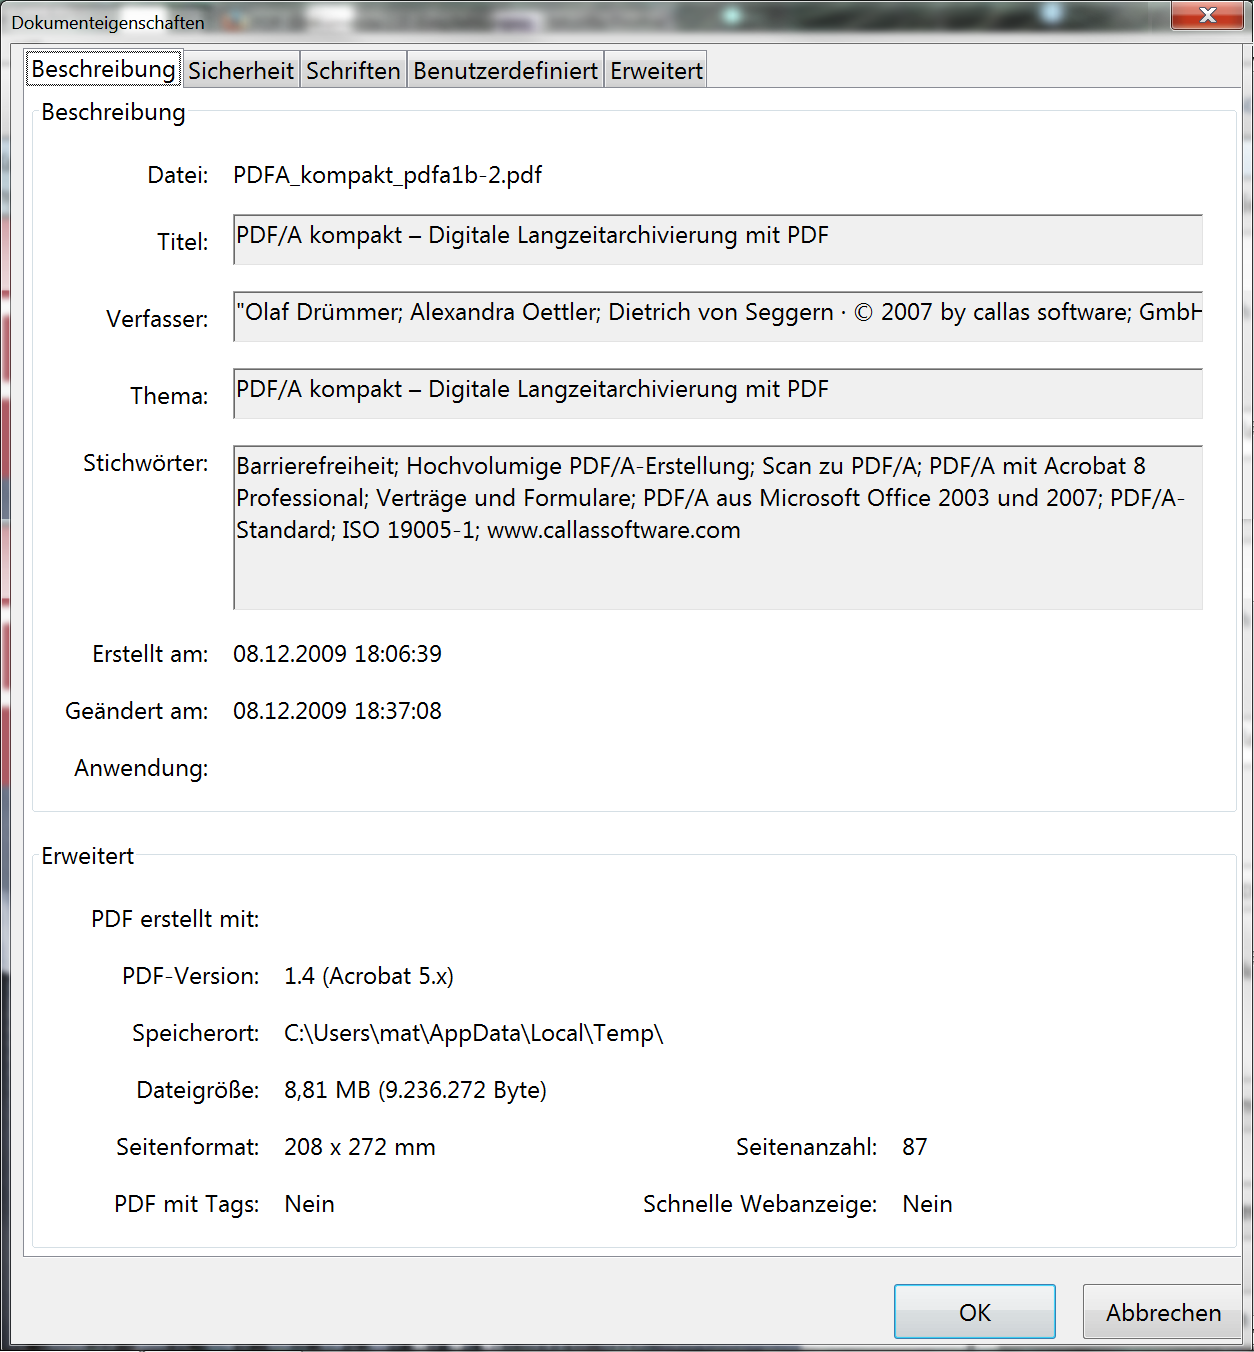
\includegraphics[width=0.9\textwidth]{bilder/doku_AdobeEigenschaften}
  \end{center}
  \caption{Beispiel der Metadaten eines PDF-Dokumentes im Programm Adobe Reader. Die Metadaten können unter "`Datei > Eigenschaften"' angezeigt und verändert werden.}
  \label{eigenschaftenAcrobat}
\end{figure}

Bei textbasierten (insbesondere XML-basierten) Dateiformaten oder Textdateien, die Auszeichnungssprachen verwenden (wie etwa SVG-, HTML- oder XML-Dateien), können Metadaten leicht mittels Auszeichnungselementen im Header der Datei integriert werden. Konkrete Hinweise für die Bearbeitung und Ergänzung von Metadaten für bestimmte Dateiformate sind in den entsprechenden Abschnitten im Kapitel Dateiformate ab Seite \pageref{dateiformate} zu finden. Auch Hinweise für die Extraktion von Metadaten in separate Dateien sind ebenfalls in den entsprechenden Abschnitten zu finden.

Für Dateiformate, in denen kein eigener Metadatenbereich vorgesehen ist, oder für übergeordnete projekt- und methodenbezogene Metadaten, ist eine Speicherung in separaten Dateien oder Systemen erforderlich. Hierfür eignen sich Tabellen und Datenbanken, da diese die Erfassung mithilfe spezifischer Eingabemasken, einer gezielten Suche und einer strukturierten Sicherung von Metadaten erleichtern. Zusätzlich erlauben sie eine (Teil-)Automatisierung der Metadaten, wie etwa die automatische Speicherung des Datums der letzten Bearbeitung eines Datensatzes und den Namen des Bearbeiters. Ein weiterer Vorteil der Erfassung von Metadaten in Tabellen oder Datenbanken besteht in der effizienten Bearbeitung von Merkmalen, die für mehrere Dokumente identisch sind, wie beispielsweise der gleiche Maßstab für alle Zeichnungen eines Projektes.

Bei der Speicherung von Metadaten in separaten Dateien muss in besonderer Weise darauf geachtet werden, dass die Beziehungen zwischen beiden Einheiten eindeutig und aktuell sind. Wird etwa bei den Metadaten der Name einer Datei zur Identifizierung verwendet, muss sichergestellt werden, dass dieser einmalig ist (ggf. in Kombination mit seinem Speicherort) und dass im Falle der Umbenennung der Datei der Eintrag auch bei den Metadaten aktualisiert wird.

Die Erfassung von Metadaten in einer Freitextdatei sollte vermieden werden, da diese meist nicht automatisiert durch Computer überprüft und verarbeitet werden können.

Bei Dokumenten mit Textinhalt können beschreibende Metadaten auch automatisch erzeugt werden, indem nach charakteristischen Zeichenketten gesucht wird und Schlag- und Stichworte extrahiert werden. Allerdings reicht die Qualität einer automatischen Erschließung bislang nicht an eine manuelle und intellektuelle Metadatenvergabe heran, da maschinell nicht nur sinnvolle Deskriptoren herausgefiltert werden.

Für die Übergabe von Dateien und Metadaten an ein Langzeitarchiv gilt die Empfehlung, die Metadaten sowohl in den Originaldateien selbst als auch in einem separaten, strukturierten und textbasierten Dokument vorzuhalten: in den Originaldateien selbst, um keine verwaisten, also undokumentierten Werke zu erzeugen, und als separate Textdatei, um eine automatisierte Verarbeitung und den Austausch von Referenzangaben zu vereinfachen.
\subsection{Metadaten in der Anwendung}
\label{Metadaten-anwendung}
\paragraph{Projektbezogene Metadaten}
Die wichtigsten Metadaten, die für die Beschreibung eines Projektes oder einer Dokumentensammlung erforderlich sind, werden in der folgenden Tabelle abgebildet und knapp definiert. Sie geben einen Überblick über einen größeren, zusammenhängenden Datenbestand und beschreiben den fachlichen Kontext in dem dieser entstanden ist. Vergleichbar einem Bibliothekskatalog liegt die Hauptfunktion dieser Metadaten darin, dass externe Personen ein Projekt oder eine dessen digitale Daten über Web-Portale und Suchmaschinen finden und einordnen können. Darüber hinaus enthalten sie rechtliche Informationen, die für den weiteren Umgang mit den Daten wichtig sind. 

Die hier vorgestellten Eigenschaften basieren auf dem Dublin Core Metadata Schema und den Angaben, wie sie vom ADS in den UK und tDAR in den USA erhoben werden, um einen zukünftigen Austausch zu vereinfachen. Ein darauf aufbauendes ausführliches Metadatenschema, das auch die Grundlage für die Archivierung von Projektdaten bei IANUS bildet, sowie ausgefüllte Beispielformulare sind in dem Kapitel Archivierung von Forschungsdaten in IANUS ab Seite \pageref{archivierungIANUS} zu finden.

\begin{center}
	\begin{longtable}{L{0.25\textwidth} p{0.68\textwidth}}
		\toprule
		Bezeichnung & Kurzdefinition\\ \midrule \endfirsthead
		\multicolumn{2}{l}{\footnotesize Fortsetzung der vorhergehenden Seite}\\
		\toprule
		Bezeichnung & Kurzdefinition\\ \midrule \endhead
		\bottomrule \multicolumn{2}{r}{{\footnotesize Fortsetzung auf der nächsten Seite}} \\
		\endfoot
		\bottomrule 
		\endlastfoot

		Identifizierung -- Projekttitel & Verbindliche Kurzbezeichnung des Projektes.\\
		Identifizierung -- Alternativtitel & Ggf. alternative Titel für ein Projekt.\\
		Identifizierung -- Projektnummer(n) & Nummern oder Kennungen, die z.B. innerhalb der durchführenden Organisation oder von Mittelgebern verwendet werden, um das Projekt eindeutig identifizieren zu können.\\
		Kurzbeschreibung & Knappe Angaben zur Fragestellung, zum Verlauf und Ergebnis des Projektes sowie Skizzierung der Datensammlung (insgesamt ca. 100-300 Worte)\\
		Schlagworte -- Fachdisziplinen & Stichworte, die die beteiligten Disziplinen und Fächer benennen. Sofern die Stichworte auf publizierten Standards oder internen Thesauri beruhen, müssen diese mitangegeben werden.\\
		Schlagworte -- Inhalt & Stichworte, die den Inhalt der Datensammlung benennen., z. B. zu Materialgruppen, Fundstellen-Klassifizierung, Quellenarten,  Kulturgruppen etc. Sofern die Stichworte auf publizierten Standards oder internen Thesauri beruhen, müssen diese mitangegeben werden.\\
		Schlagworte -- Methoden & Stichworte, die die eingesetzten Forschungsmethoden beschreiben. Sofern die Stichworte auf publizierten Standards oder internen Thesauri beruhen, müssen diese mitangegeben werden.\\
		Ausdehnung -- Geografisch-1 & Detaillierte Angaben zur räumlichen Ausdehnung oder zum Fundort des untersuchten Gegenstandes mittels geografischer Koordinaten. Die maximale Ausdehnung kann als Bounding Box angegeben werden.\\
		Ausdehnung -- Geografisch-2 & Sprachliche Beschreibung des untersuchten Gegenstandes mittels Ortsangaben mit Land, Stadt, Kreis, Straße, Gemarkung etc. Sofern Namen sich im Lauf der Zeit geändert haben, dies gesondert vermerken. Sofern eine Referenz zu einer Geo-Ressource oder einem Gazetteer existiert, sollte diese ebenfalls angegeben werden.\\
		Ausdehnung -- zeitlich & Chronologische Angaben zum untersuchten Gegenstand, entweder als Periodenbezeichnung und/oder mit groben/genauen Jahresangaben. Sofern die Stichworte auf publizierten Standards oder internen Thesauri beruhen, müssen diese mitangegeben werden.\\
		Primärforscher -- Person & Personen, die entweder für das Projekt als Ganzes, für das Datenmanagement oder für die Erzeugung bestimmter Datenarten zentral bzw. verantwortlich sind. Hier ist eine Kontaktadresse erforderlich und die aktuelle/letzte institutionelle Zugehörigkeit, damit die Personen bei Rückfragen erreicht werden kann.\\
		Eigentümer -- Organisation & Organisation, der die unter "`Primärforscher"' genannten Personen angehören, oder die nach Ausscheiden derselben für die Daten verantwortlich ist, im weitesten Sinne also Eigentümer der Daten ist. Hier ist eine Kontaktadresse erforderlich, damit die Organisation bei Rückfragen erreicht werden kann.\\
		Finanzierung & Nennung der Organisation(en) / (Dritt-)Mittelgeber, durch die das Projekt finanziert wurde. Es sollte jeweils der Zeitraum der Finanzierung angegeben werden.\\
		Veröffentlichung -- Projektdaten & Wenn die hier beschriebene Datensammlung des Projektes bereits an anderer Stelle veröffentlicht / online gestellt wurde, bitte entsprechende Angaben machen, z. B. durch Nennung der Organisationen, Datenarchive, Online-Ressourcen etc.\\
		Veröffentlichung -- Ergebnisse & Analoge oder digitale Publikationen zu Ergebnissen des Projektes oder zur Datensammlung des Projektes, ausführliche bibliographische Angaben (ohne fachspezifische Abkürzungen) unter Nennung des Verlages erforderlich.\\
		Dauer -- Projekt & Anfangs- und Enddatum des Projektes.\\
		Dauer -- Datenbestand & Anfangs- und Enddatum der Erzeugung oder Verarbeitung digitaler Daten im Rahmen des Projektes.\\
		Rechtliches -- Urheberrechte & Name des Inhabers der Urheber-, Nutzungs- und Verwertungsrechte; i. d. R. die Organisation, an der der Primärforscher beschäftigt war.\\
		Rechtliches -- Lizenzgeber & Angabe der Person, die i. d. R. als Vertretung für eine Organisation für die Lizenzierung von Daten zur Nachnutzung verantwortlich und berechtigt ist, einen Datenübergabevertrag abzuschließen.\\
		Rechtliches -- Datenschutz & Angaben, ob in der Datensammlung datenschutzrelevante Informationen enthalten sind. Wenn ja, in welchem Umfang.\\
		Quellen -- Ältere & Ältere Quellen oder existierende Ressourcen, auf denen die Daten aufbauen.\\
		Quellen -- Zugehörige & Sofern während des Projektes Informationen, Datensammlungen, (un-)publizierte Dokumente, Online-Ressourcen etc. verwendet oder erzeugt wurden, die nicht Teil der hier beschriebenen Datensammlung sind, aber für deren Verständnis wichtig sind, bitte entsprechende Angaben zu Art und Umfang dieser Quellen machen.\\
		Sprache & Die in den Dokumenten und Dateien verwendete(n) Sprache(n). Sprachkennungen nach ISO 639 angeben.\\
		Art der Daten & Kurzcharakterisierung der Daten, z. B. ob es sich um Rohdaten, verarbeitete Daten, Interpretationen, Ergebnisse, Abschlussberichte etc. handelt.\\
		Vollständigkeit & Aussagen zur Vollständigkeit der Projektdaten, z. B. ob bestimmte Datenarten noch fehlen und warum.\\
		Dateiformate & Auflistung der Dateiformate, die in der Datensammlung vorkommen, ggf. unter Nennung der verwendeten Programme und Zeichenkodierungen.\\
		Zugriffsrechte & Festlegung der gewünschten Zugriffsrechte für die Daten, sofern diese für den gesamten Projekt-Datenbestand gelten sollen; differenzierte Regelungen müssen auf Dateiebene vorgenommen werden.\\
		Signatur Metadaten & Angabe darüber, wer die o. g. Metadaten wann ausgefüllt hat.\\
		\bottomrule
	\end{longtable}
\end{center}

\paragraph{Dateibezogene Metadaten}
Bei dieser Art von Metadaten handelt es sich um technische und inhaltliche Informationen, die Nutzern verständlich machen, wie einzelne Dateien innerhalb eines Projektes oder einer Datensammlung beschaffen sind und welche Möglichkeiten der Nachnutzbarkeit sie beinhalten. 

Dateibezogene Metadaten sind abhängig von dem Format, dem Inhalt und der Methode, mit denen die Dateien erzeugt wurden. Beispielsweise sind für Rastergrafiken, die durch digitale Fotografie entstanden sind, andere Angaben erforderlich (Fotograf, Aufnahmedatum, Aufnahmeort, abgelichtetes Objekt etc.) als für Rasterdateien, die durch geophysikalische Messungen erzeugt wurden (Koordinaten, Messgerät, Genauigkeit, Datum etc.). Zusätzliche spezifische Angaben, die für bestimmte Dateiformate empfohlen werden, sind in den verschiedenen Kapiteln zu den jeweiligen Formaten ab Seite \pageref{dateiformate} beschrieben.

Es gibt jedoch dateibezogene Metadaten, die unabhängig von Format, Inhalt und Methode für alle Einzeldateien gleichermaßen relevant und notwendig sind. Zu diesen Metadaten gehören neben den Angaben zu Dateiname, Dateiformat, Dateiversion, Titel, Beschreibung und Ersteller auch Informationen zur verwendeten Soft- und Hardware, Versionierung, zu rechtlichen Aspekten und Verweise auf weitere relevante Dateien.

Auch wenn es in der Theorie wünschenswert ist, diese Angaben sowie die zugehörigen spezifischen Angaben zu Methoden und Dateiformaten für jede Datei einzeln zu erfassen, so zeigt die Praxis, dass es häufig ausreichend ist, einen Metadatensatz für Gruppen von Dateien anzulegen, wenn diese das gleiche Format oder die gleichen inhaltlichen Eigenschaften aufweisen. 

\begin{center}
	\begin{longtable}{L{0.25\textwidth} p{0.68\textwidth}}
		\toprule
		Bezeichnung & Kurzdefinition\\ \midrule \endfirsthead
		\multicolumn{2}{l}{\footnotesize Fortsetzung der vorhergehenden Seite}\\
		\toprule
		Bezeichnung & Kurzdefinition\\ \midrule \endhead
		\bottomrule \multicolumn{2}{r}{{\footnotesize Fortsetzung auf der nächsten Seite}} \\
		\endfoot
		\bottomrule 
		\endlastfoot
		
		Identifikator, Dateiname & Eindeutiger Name der Datei.\\
		Dateiformat & Format, in dem die Datei abgespeichert ist.\\
		Urheber & Name des Verfassers oder Erstellers der Datei.\\
		Titel & Titel der Datei, nicht der Dateiname.\\
		Beschreibung & Beschreibung des Inhalts der Datei. \\
		Schlagworte & Schlagworte, wie etwa Periode, Fundstelle oder charakteristische Merkmale. Wenn vorhanden, angemessene Thesauri verwenden.\\
		Software -- Dateierstellung & Software, mit der die Datei erstellt wurde.\\
		Hardware -- Dateierstellung & Hardware, mit der die Datei erstellt wurde, v. a. bei technischen Geräten wie Kameras, GPS-Geräten, Vermessungsinstrumenten, Laserscanner etc.\\
		Betriebssystem -- Dateierstellung & Betriebssystem, das verwendet wurde als die Datei erstellt wurde.\\
		Erstellungsdatum & Datum, an dem die Datei erstellt wurde. Datum und Zeit in UTC nach ISO 8601.\\
		Letzte Aktualisierung & Datum, an dem die Datei zuletzt bearbeitet wurde. Datum und Zeit in UTC nach ISO 8601.\\
		Dateiversion & Angabe der Versionsnummer der Datei.\\
		Weitere Dateien & Referenzen auf Dateien, die für das Verständnis einer anderen Datei zentral sind, insbesondere für zusammenhängende, komplexe Dateien oder wenn auf eine Ursprungsdatei verwiesen werden soll.\\
		Sprache & Sofern schriftliche Inhalte vorhanden sind, die Sprache angeben. Sprachkennungen nach ISO 639 angeben.\\
		Copyright-Angaben & Angaben zur Person oder Einrichtung, die das Copyright oder die Lizenzrechte an der Datei oder deren Inhalt besitzt.\\
		\bottomrule
	\end{longtable}
\end{center}

\paragraph{Methodenbezogene Metadaten}
Jede Fachdisziplin innerhalb der Altertumswissenschaften verfügt über spezifische Forschungsmethoden. Auch diese haben Einfluss auf Umfang, Art, Struktur und Inhalt digitaler Objekte, da sie bei verschiedenen Arbeitsweisen und technischen Geräten unterschiedlich ausfallen. Daher sollten methodenbezogene Metadaten ebenfalls dokumentiert werden, insbesondere wenn mehrere Zwischenstände einer Prozesskette archiviert und Dritten zur Verfügung gestellt werden sollen. Je nach Genauigkeit der Methodenbeschreibung kann sie sich sowohl auf eine Einzeldatei als auch auf mehrere Dateien gleichen Typs beziehen.

Die Angabe der methodenbezogenen Metadaten ist wichtig, um zu beschreiben, wie die Rohdaten in prozessierte Daten überführt wurden. Außerdem kann so verstanden werden, welchen Einfluss die angewandte Methode auf das Ergebnis hat, das Ergebnis folglich zu interpretieren ist und wo Fehler zu erwarten sind.

Zusätzliche spezifische Angaben, die für bestimmte Forschungsmethoden oder Prozesse empfohlen werden, sind in den einzelnen Kapiteln des Abschnittes Forschungsmethoden ab Seite \pageref{methoden} beschrieben.

\begin{center}
	\begin{tabular}{L{0.25\textwidth} p{0.68\textwidth}}
		\toprule
		Bezeichnung & Kurzdefinition\\ \midrule
		Prozessnummer & Eindeutige Nummer eines Prozesses oder einer Methode.\\
		Prozessbeschreibung & Beschreibung des Prozesses oder der Methode. Insbesondere Beschreibung der Ausgangssituation und der Zielvorstellung.\\
		Ausgangsformat(e) & Format der Dateien, die am Anfang eines gesamten Prozesses stehen und den Ausgangspunkt bilden.\\
		Zwischenformat(e) & Format der Dateien, die im Verlauf eines Prozesses erzeugt werden und den Ausgangspunkt für weitere Prozesse bilden.\\
		Zielformat(e) & Format der Dateien, die am Ende eines Prozesses erzeugt werden.\\
		Durchführender & Person(en), die den Prozess durchgeführt hat (haben).\\
		Prozessbeginn & Datum, an dem der Prozess begonnen wurde. Datum und Zeit in UTC nach ISO 8601.\\
		Prozessende & Datum, an dem der Prozess beendet wurde. Datum und Zeit in UTC nach ISO 8601.\\
		Software & Software, mit der der Prozess durchgeführt wurde.\\
		Hardware & Hardware, auf der der Prozess durchgeführt wurde.\\
 		\bottomrule
		\bottomrule
	\end{tabular}
\end{center}


%##################################################################################
\label{grabungsdokumentation}
\subsection{Grabungsdokumentation}
Speziell für die Dokumentation von Grabungen und anderen archäologischen Maßnahmen sind weitere Metadaten erforderlich, die in der folgenden Tabelle aufgelistet sind. Dabei sollten auch die verschiedenen angewandten Methoden berücksichtigt werden, da diese ebenfalls den Umfang und die Art der Dokumentation beeinflussen. Wichtig bei einer Grabungsdokumentation ist, dass nicht nur die digitalen Daten, sondern auch die analogen Daten mit einer Dokumentation versehen sind, um beispielsweise auch Abhängigkeiten zwischen den verschiedenen Daten festzuhalten. Zum Beispiel sollten Zeichnungen mit den Befundbeschreibungen, Fotos mit den Fundstellenplänen oder Objektbeschreibungen mit den jeweiligen Objekten verknüpft sein.

\begin{center}
	\begin{longtable}{L{0.25\textwidth} p{0.68\textwidth}}
		\toprule
		Bezeichnung & Kurzdefinition\\ \midrule \endfirsthead
		\multicolumn{2}{l}{\footnotesize Fortsetzung der vorhergehenden Seite}\\
		\toprule
		Bezeichnung & Kurzdefinition\\ \midrule \endhead
		\bottomrule \multicolumn{2}{r}{{\footnotesize Fortsetzung auf der nächsten Seite}} \\
		\endfoot
		\bottomrule 
		\endlastfoot

		Fundstellenart & Angabe über die Art der Fundstelle. Mehrfachangaben sind möglich, wenn beispielsweise ein sich mit einer Siedlung überlagerndes Gräberfeld beschrieben werden soll.\\
		Maßnahmenart & Angabe über die Art der Untersuchung. Werte können beispielsweise sein: Ausgrabung, Survey, Baustellenbegleitung etc.\\
		Anlass & Angabe des Anlasses, der zur Durchführung der Maßnahme führt. Werte können beispielsweise sein: Rettungsgrabung, Notgrabung, Forschungsgrabung, Lehrgrabung etc.\\
		Grabungsmethodik & Angabe der angewandten Grabungsmethodik. Werte können beispielsweise sein: Flächengrabung, Schichtengrabung, Wheeler-Kenyon-Methode etc.\\
		Verfahren & Angabe über die angewandten Arbeitsverfahren, die nicht zu Dokumentationsverfahren gehören. Werte können beispielsweise sein: Schlämmen, Bohrung, Sieben etc.\\
		Datierung & Datierung der Fundstelle, beispielsweise anhand des archäologischen Fundmaterials. Eingruppierung in eine Epoche als relative Zeitstellung und optional als absolute Zeitangabe. Bei mehrphasigen Fundstellen werden mehrere Zeiträume angegeben.\\
		Fundstellenstatus & Angaben zum Schutzstatus einer Fundstelle.\\
		Bodenbeschaffenheit & Angabe über die natürlichen Gegebenheiten und die Bodenbeschaffenheit, die Einfluss auf die Erhaltungsbedingungen von Objekten und Strukturen haben. Werte können beispielsweise sein: Feuchtboden, Mineralboden, Unter Wasser etc.\\
		Strukturen & Verschlagwortung von aufgefundenen archäologischen Strukturen, die sich aus den Befunden ergeben.\\
		Funde & Verschlagwortung von signifikanten Fundgattungen.\\
		Richtlinie & Angaben zur Grabungs- oder Dokumentationsrichtlinie, die für die Maßnahme vorgegeben war oder gewählt wurde.\\
		Dokumentationssystem & Angabe des verwendeten Dokumentationssystems. Werte können beispielsweise sein: Stellenkartensystem, Single Context Recording, spezielle institutionelle Systeme etc.\\
		Dokumentationsmethoden & Angabe der verwendeten Dokumentationsmethoden. Werte können beispielsweise sein: Text, Foto, Zeichnung, 3D-Scan, Vermessung etc. \\
		\bottomrule
	\end{longtable}
\end{center}

Die große Zahl an Dokumentationsverfahren und Forschungsmethoden führt dazu, dass eine umfassende Grabungsdokumentation aus einer großen Menge unterschiedlicher Dokumente besteht, die folgendes enthalten sollte:
\begin{itemize}
	\item Allgemeine Angaben
	\item Grabungsplan
	\item Grabungstagebuch und Grabungsprotokoll
	\item Befundblätter und Befundliste
	\item Fundzettel und/oder Fundmeldung
	\item Fund- und Probenliste
	\item Datenbanken
	\item Dokumentation der angewandten Methoden, wie:
	\begin{itemize}
		\item Vermessungsmethoden
		\item Fotografie
		\item Photogrammetrie
		\item 3D-Scans
		\item Luftbildaufnahmen
		\item Naturwissenschaftliche Beprobung
		\item Zeichnung
		\item Allgemeine Beschreibungen
	\end{itemize}
	\item Abschlussbericht
\end{itemize}

Wie eine Grabungsdokumentation aussehen und welchen Umfang sie haben soll, wird in zahlreichen Richtlinien und Vorgaben spezifiziert, die bei der Planung des Vorhabens bereits berücksichtigt werden sollten. Dabei handelt es sich meist um Vorgaben von Landesdenkmalämtern. Online verfügbare Vorgaben sind bei den weiterführenden Informationen unter Vorgaben zur Grabungsdokumentation ab Seite \pageref{Metadaten-ListeLDA} aufgelistet.

Um die Grabungsdokumentation zu erleichtern und auch sicher zu stellen, dass alle erforderlichen Metadaten angegeben werden, sollten Vorlagen für Formulare und Checklisten bereits vor der Durchführung der Maßnahme erstellt werden. In der online verfügbaren Fassung der IT-Empfehlungen sind zu diesem Kapitel passende Vorlagen zur freien Verwendung zu finden. Darunter befinden sich eine Befundliste, eine Fotoliste, eine Fundliste, eine Geräteliste, ein Probenverzeichnis, ein Restaurierungsverzeichnis, ein Zeichnungsverzeichnis und ein Dokument zur Urheberrechtsverwaltung. Ein weiterer Anhaltspunkt sind die bereits genannten Richtlinien, sowie das Werk "`Tabellen und Tafeln zur Grabungstechnik"' von Andreas Kinne und das Grabungstechnikerhandbuch des Verbandes der Landesarchäologen. 
\newpage
\subsection{Weiterführende Informationen}
\begin{flushleft}
\quelltyp{Metadaten allgemein}
Archaeology Data Service: Guides to Good Practice -- Project Metadata \urllist{http://guides.archaeologydataservice.ac.uk/g2gp/CreateData\_1-2}

Archaeology Data Service: Project metadata for the Archaeology Data Service \urllist{https://archaeologydataservice.ac.uk/resources/images/attach/ADS_collection_level_metadata_example.pdf}

DARIAH-DE (Hrsg.) Daten- und Metadatenformate in den Fachdisziplinen. Archäologie (2015) \urllist{http://dev2.dariah.eu/wiki/pages/viewpage.action?pageId=20058856}

Deutsche Initiative für Netzwerkinformation e. V. (Hrsg.) Kompetenzzentrum Interoperable Metadaten (KIM) \urllist{http://www.dini.de/ag/standards/}

Gesis: Dokumentation und Metadaten \urllist{https://web.archive.org/web/20150928031540/http://www.gesis.org/archive-and-data-management-training-and-information-center/forschungsdatenmanagement/dokumentation-und-metadaten/}

U. Jensen -- A. Katsanidou -- W. Zenk-Möltgen, Metadaten und Standards, in: S. Büttner -- H.-C. Hobohm -- L. Müller (Hrsg.) Handbuch Forschungsdatenmanagement (Bad Honnef 2011) 83-100 \urllist{http://www.forschungsdatenmanagement.de/?page_id=2}

A. Kinne, Tabellen und Tafeln zur Grabungstechnik (Dresden 2013)\abstand

J. M. Lill, Kontrolliertes Vokabular. Wieso? Weshalb? Warum?, Fachgruppe Dokumentation im DMB: Terminologie -- das Schweizer Messer der Dokumentation (9. Mai 2012, Kunstmuseum Stuttgart) \urllist{http://swop.bsz-bw.de/volltexte/2012/1002/pdf/Lill_Textfassung_VortragDMB2012.pdf}

J. Lindenthal, Normen und Standards für Thesauri (2015) \urllist{https://www.ianus-fdz.de/it-empfehlungen/sites/default/files/NormenEmpfehlungenEntwicklungThesauri_Lindenthal.pdf}

nestor (Hrsg.) Standardisierung -- Metadaten \urllist{https://wiki.dnb.de/display/NESTOR/Metadaten}

C. Papatheodorou -- D. Gavrilis -- K. Fernie -- H. Wright -- J. Richards -- P. Ronzino -- C. Meghini, D3.1 Initial Report on the project registry (2013)\urllist{http://ariadne-infrastructure.eu/Resources/D3.1-Initial-Report-on-the-project-registry}

National Information Standards Organization (Hrsg.) Understanding Metadata \urllist{http://www.niso.org/publications/press/UnderstandingMetadata.pdf}

J. Riley -- D. Becker, Glossary of Metadata Standards (2010) \urllist{http://jennriley.com/metadatamap/seeingstandards_glossary_pamphlet.pdf}

Verband der Landesarchäologen (Hrsg.) Grabungstechnikerhandbuch \urllist{http://www.landesarchaeologen.de/verband/kommissionen/grabungstechnik/grabungstechnikerhandbuch/}

W3C (Hrsg.) Vocabularies \urllist{http://www.w3.org/standards/semanticweb/ontology}

\quelltyp{Metadatenschemata}
Dublin Core Metadata Initiative: \urllist{http://dublincore.org/}

OASIS (Version 1.3): \urllist{http://oasis.ac.uk/pages/wiki/TECHNICAL\%20INFORMATION}

ADeX -- Standard für den Austausch archäologischer Fachdaten: \urllist{http://www.landesarchaeologen.de/verband/kommissionen/archaeologie-und-informationssysteme/projektearbeitsgruppen/adex/}

CARARE metadata schema: \urllist{http://pro.carare.eu/doku.php?id=support:metadata-schema}

IANUS: \urllist{https://www.ianus-fdz.de/it-empfehlungen/archivierung}

CIDOC Conceptual Reference Model (Vers. 5.0.4): \urllist{http://www.cidoc-crm.org/}

CIDOC-CRM, CRMarchaeo, CRMba, CRNdig und CRMgeo: \urllist{http://www.cidoc-crm.org/collaborations}

Ariadne Reference Model: \urllist{http://www.ariadne-infrastructure.eu/Resources/Ariadne-Reference-Model}

LIDO Lightweight Information Describing Objects: \urllist{http://network.icom.museum/cidoc/working-groups/lido/lido-technical/specification/}

MIDAS Heritage: \urllist{http://heritage-standards.org.uk/midas-heritage/}

\quelltyp{Kontrollierte Vokabulare, Thesauri und Normdaten}
Art \& Architecture Thesaurus (AAT): \urllist{http://www.getty.edu/research/tools/vocabularies/aat/}

Heritage Data -- Linked Data Vocabularies for Cultural Heritage: \urllist{http://www.heritagedata.org/blog/vocabularies-provided/}

Wortnetz Kultur (WNK): \urllist{http://www.digicult-verbund.de/vortraege/2015/WNK_WortnetzKultur_20151110.pdf} \vspace{-0.2cm} \hspace{0.2cm}\url{http://www.lvr.de/de/nav_main/kultur/kulturwissen/digitales_kulturerbe/digitales_kulturerbe_1.jsp}\vspace{0.1cm}

iDAI.vocab: \urllist{http://archwort.dainst.org/}

iDAI.thesaurus: \urllist{http://thesauri.dainst.org/de/hierarchical_concepts.html}  

Encyclopedia of Life: \urllist{http://eol.org/}

Wikidata: \urllist{https://www.wikidata.org/wiki/Wikidata:Main_Page}

GeoNames: \urllist{http://www.geonames.org/}

iDAI.gazetteer: \urllist{https://gazetteer.dainst.org/}

Pleiades: \urllist{https://pleiades.stoa.org/} 

Getty Thesaurus of Geographic Names (TGN): \urllist{http://www.getty.edu/research/tools/vocabularies/tgn/} 

PeriodO: \urllist{http://perio.do/}

iDAI.chronontology: \urllist{http://chronontology.dainst.org/}

Virtual International Authority File (VIAF): \urllist{http://viaf.org/}

Open Researcher and Contributor ID (ORCID): \urllist{https://orcid.org/}

Gemeinsame Normdatei (GND): \urllist{http://www.dnb.de/DE/Standardisierung/GND/gnd_node.html}

Katalog der Deutschen Nationalbibliothek: \urllist{http://www.dnb.de/}

iDAI.bibliography (Zenon): \urllist{https://zenon.dainst.org/}

\label{Metadaten-ListeLDA}
\quelltyp{Vorgaben zur Grabungsdokumentation}
ARCHES: Archäologische Archivierung in Europa: Ein Handbuch (EAC-Guidelindes 1): \urllist{http://www.europae-archaeologiae-consilium.org/eac-guidlines}

Verband der Landesarchäologen: \urllist{www.landesarchaeologen.de/fileadmin/Dokumente/Dokumente_Kommissionen/Dokumente_Grabungstechniker/grabungsstandards_april_06.pdf}

Bayerische Landesamt für Denkmalpflege: \urllist{http://www.blfd.bayern.de/bodendenkmalpflege/service/}\vspace{-0.2cm} \hspace{0.2cm}\url{http://www.blfd.bayern.de/medien/dokuvorgaben_august_2016.pdf}\vspace{0.1cm}

Landesdenkmalamt Berlin: \urllist{http://www.stadtentwicklung.berlin.de/denkmal/landesdenkmalamt/download/neuerscheinungen/grabung_standard.pdf}

Brandenburgisches Landesamt für Denkmalpflege: \urllist{https://www.bldam-brandenburg.de/bodendenkmalpflege}

Archäologisches Museum Hamburg: \urllist{http://amh.de/wp-content/uploads/DokumtationsrichtlinienHamburg.pdf}

Landesamt für Denkmalpflege Hessen: \urllist{https://lfd.hessen.de/sites/lfd.hessen.de/files/content-downloads/hA_Grabungs-Dokurichtlinien_2015.pdf}

Niedersächsisches Landesamt für Denkmalpflege: \urllist{https://www.denkmalpflege.niedersachsen.de/download/110131}

LVR-Amt für Bodendenkmalpflege im Rheinland: \urllist{http://www.bodendenkmalpflege.lvr.de/de/service/grabungsrichtlinien/grabungsrichtlinien_1.html}

Generaldirektion Kulturelles Erbe Rheinland-Pfalz: \urllist{http://download.gdke-rlp.de/archaeologie/richtlinien_ausgrabung.pdf}

Zeichenrichtlinien des Landesamtes für Denkmalpflege und Archäologie Sachsen-Anhalt: \urllist{www.lda-lsa.de/fileadmin/bilder/dienste/redaktion/Zeichenrichtlinie.pdf}

Bundesdenkmalamt Österreich: Richtlinien für Archäologische Massnahmen \urllist{https://bda.gv.at/de/publikationen/standards-leitfaeden-richtlinien/richtlinien-fuer-archaeologische-massnahmen/}

Eine Liste weiterer Richtlinien bei Archäologie Online: \urllist{http://www.archaeologie-online.de/links/236/592/659/index.php} 
\end{flushleft}

\newpage
\section{Dateiverwaltung}\label{dateiverwaltung}
\abschnittsautor{M. Trognitz, F. Schäfer, R. Göldner, T. Schenk}
\hyphenation{
Schnitt-stel-le
}
Der tägliche Umgang mit digitalen Daten wird durch eine effiziente Dateiverwaltung erheblich erleichtert. Aussagekräftige Dateinamen, die auch für Dritte verständlich sind, sorgen dafür, dass die Dateien gefunden und deren Inhalt verstanden wird. Einheitliche Dateinamensstrukturen erhöhen die Lesbarkeit. Die konsequente Einhaltung von Versionierungsangaben sorgt dafür, dass immer mit der richtigen Dateiversion gearbeitet wird und eine selbsterklärende Ordnerstruktur hilft dabei auch in großen Projekten bestimmte Dateien wiederzufinden.

Die Konzipierung der Dateiverwaltung muss schon zu Beginn des Projektes erfolgen, damit die Regeln von Anfang an angewendet werden können. Die Niederschrift der durch Beispiele ergänzten Benennungsregeln und deren Weitergabe dient im laufenden Betrieb als wichtiges Nachschlagewerk für die konsistente und konsequente Einhaltung derselben. Dies ermöglicht eine effizientere Arbeitsweise.

Im laufenden Projektbetrieb sollte die Einhaltung der Benennungsregeln kontrolliert und gegebenfalls angepasst werden.


\subsection{Dateiablage}
Mit Dateiablage ist hier vor allem die Ordnerstruktur gemeint. Für die Benennung der Ordner gelten die gleichen Regeln, wie für die Dateibenennung, die im Abschnitt Dateibenennung ab Seite \pageref{dateibenennung} thematisiert werden. Lediglich die Dateinamenserweiterung wird bei Ordnernamen nicht verwendet. Die Dateiablage sollte selbsterklärend sein und unpräzise Namen wie etwa \emph{"`In Arbeit"'} vermieden werden.

Wichtig ist, dass die Dateiablage logisch und hierarchisch aufgebaut ist, damit andere Nutzer die gewünschten Informationen finden und einordnen können. Dies bedeutet unter anderem, dass die Inhalte und Unterordner auch tatsächlich thematisch in den übergeordneten Ordner hineinpassen. Beispielsweise erwartet man in einem Ordner mit dem Namen \emph{"`Fotos"'} diverse Fotos, die bei einer entsprechenden Menge vielleicht noch auf verschiedene Unterordner, wie zum Beispiel \emph{"`Plana"'} und \emph{"`Profile"'}, verteilt sind.   

Ist aber in dem Ordner \emph{"`Fotos"'} ein Unterordner mit dem Namen \emph{"`Zeichnungen"'} enthalten, in dem verschiedene digitalisierte Zeichnungen abgelegt sind, führt das zu Schwierigkeiten. Der Unterordner wird wahrscheinlich nur schwer wiedergefunden werden, da der Name des übergeordneten Ordners einen anderen Inhalt verspricht.

Tritt der Fall ein, dass eine Datei oder ein Ordner thematisch in mehrere verschiedene übergeordnete Ordner passen würde, können verschiedene Lösungswege zur Anwendung kommen. Beispielsweise könnte eine Kopie abgelegt werden, was allerdings problematisch ist, wenn eine der Kopien verändert wird und diese nicht mit der anderen abgeglichen wird.

Auch von Dateiverknüpfungen ist abzuraten, da sie meist nicht betriebssystemübergreifend funktionieren und im schlechtesten Fall nur auf dem Rechner, mit dem sie erstellt wurden, funktionieren. Wird die Datei verschoben, umbenannt oder gelöscht, so wird die Dateiverknüpfung ins Leere führen.

Eine bessere Methode ist das Anlegen einer Textdatei mit einem Hinweis auf den Ablageort der Datei oder des Ordners. In diesem Fall muss aber darauf geachtet werden, dass die gesuchte Datei sich auch tatsächlich an dem angegebenen Ort befindet. Bei Verschieben oder Löschen müsste die Textdatei also auch immer berücksichtigt und angepasst werden. 

Am besten ist es, nur eine Instanz einer Datei oder eines Ordners zu haben. Bei Zuordnungsschwierigkeiten kann es helfen, die Datei oder den Ordner in der hierarchischen Struktur höher anzusiedeln.

Eine Textdatei kann auch verwendet werden, um die vorhandene Ordnerstruktur zu erklären oder auf Besonderheiten hinzuweisen. Beispielsweise kann in einem Ordner mit Fotos, deren Metadaten in einer Datenbank abgespeichert sind, mit Hilfe einer Textdatei verdeutlicht werden, wo die Metadaten zu finden sind. Damit die Textdatei auch als eine Hilfedatei erkannt wird, kann man ihr den Namen \emph{"`README"'} oder \emph{"`LIESMICH"'} geben. Die Schreibung mit Großbuchstaben erhöht die Auffälligkeit der Datei. Durch eine vorangestellte Null oder einen vorangestellten Unterstrich kann sie auch in der Sortierung an den Anfang gestellt werden.

Mittels eines Dokumentenmangaementsystems, kann eine Dateiablage auch datenbankgestützt Verwaltet werden, was jedoch einen höheren technischen Aufwand erfordert. Der Vorteil ist, dass Dateien nach beliebigen Kriterien sortiert und gesucht werden können. Jedoch kann eine mit einem Dokumentenmanagementsystem erstellte Dateiablage ohne dieses System unter Umständen nicht mehr verständlich sein, da für die Dateien abstrakte Bezeichnungen vom System vergeben werden.

\subsection{Empfehlungen für eine Ordnerstruktur}
Die Organisation der Ordnerstruktur kann sich anhand der angewandten Prozesse oder an den Ergebnissen orientieren. Im ersten Fall bildet die Struktur zeitliche und methodische Prozesse der Daten ab, was zu einer besseren Nachvollziehbarkeit der Arbeitsschritte führt. Im zweiten Fall orientiert sich die Ordnerstruktur an den fachlichen Ergebnissen, was die inhaltliche Nachvollziehbarkeit verbessert.

Bei der Planung einer Ordnerstruktur spielen weitere Kriterien eine Rolle. Abhängig von dem Umfang und der Dauer des Projektes, kann sich die Ordnerstruktur beispielsweise am Thema, dem Material, dem Jahr, dem Bearbeiter oder den einzelnen Arbeitsschritten orientieren. Dabei sollte beachtet werden, dass die Dateiablage nicht zu verzweigt ist, da die maximale Pfadlänge, die sich aus allen enthaltenden Ordnernamen und dem Dateinamen zusammensetzt, in Windows auf 260 Zeichen begrenzt ist.

Ganz allgemein kann die oberste Hierarchie der Dateiablage nach folgenden Kriterien unterteilt werden:
\begin{itemize}
	\item Ort
	\item Fundplatz, Monumente oder Denkmäler
	\item Aktivität
	\item Projekt
\end{itemize}

Für weitere Hierarchieebenen können folgende Kriterien berücksichtigt werden:
\begin{itemize}
	\item Verfahren, wie Prospektion, Voruntersuchung oder Hauptuntersuchung
	\item Arbeitsschritte mit Bezug auf Zeit, Typ und Kennung
	\item Fachliche Inahlte, wie Befunde, Funde, Proben, Bauwerke, Berichte oder Tagebuch
	\item Methodik, wie Vermessung, Foto, Zeichnung oder Photogrammetrie
	\item Räumliche Spezifizierung, wie Planum, Schnitt oder Surveyfläche
	\item Administration
\end{itemize}

Zusätzlich sollte eine Unterscheidung zwischen originalen Daten (Rohdaten), sekundären und finalen Daten erfolgen, um Prozesse transparent abzubilden. Dies ist auch für die zu archivierenden Daten relevant, da bei der Auswahl der Daten überholte oder temporäre Dateien und Dubletten in der Regel nicht berücksichtigt werden.

Anwendungsgebiete mit mehreren voneinander abhängigen Dateikomplexen, wie zum Beispiel 3D-Scanning oder RTI-Fotografie, erfordern eigene Dateiablagen. Diese werden in den entsprechenden Abschnitten im Kapitel "`Forschungsmethoden"' ab Seite \pageref{methoden} beschrieben.
\hyphenation{
Schnitt-stel-le
}
\paragraph{Praxisbeispiele} In diesem Abschnitt werden drei Beispiele für Dateiablagen vorgestellt, die aus Baden-Württemberg, Hamburg und Österreich stammen. Das Landesdenkmalamt von Baden-Württemberg verwendet eine Dateiablage, die an der analogen Ordnerstruktur einer Grabung orientiert ist. Sie wird in Abbildung \ref{OrdnerstrukturBaWue} veranschaulicht.

\begin{figure}[h!tb]
  \begin{center}
    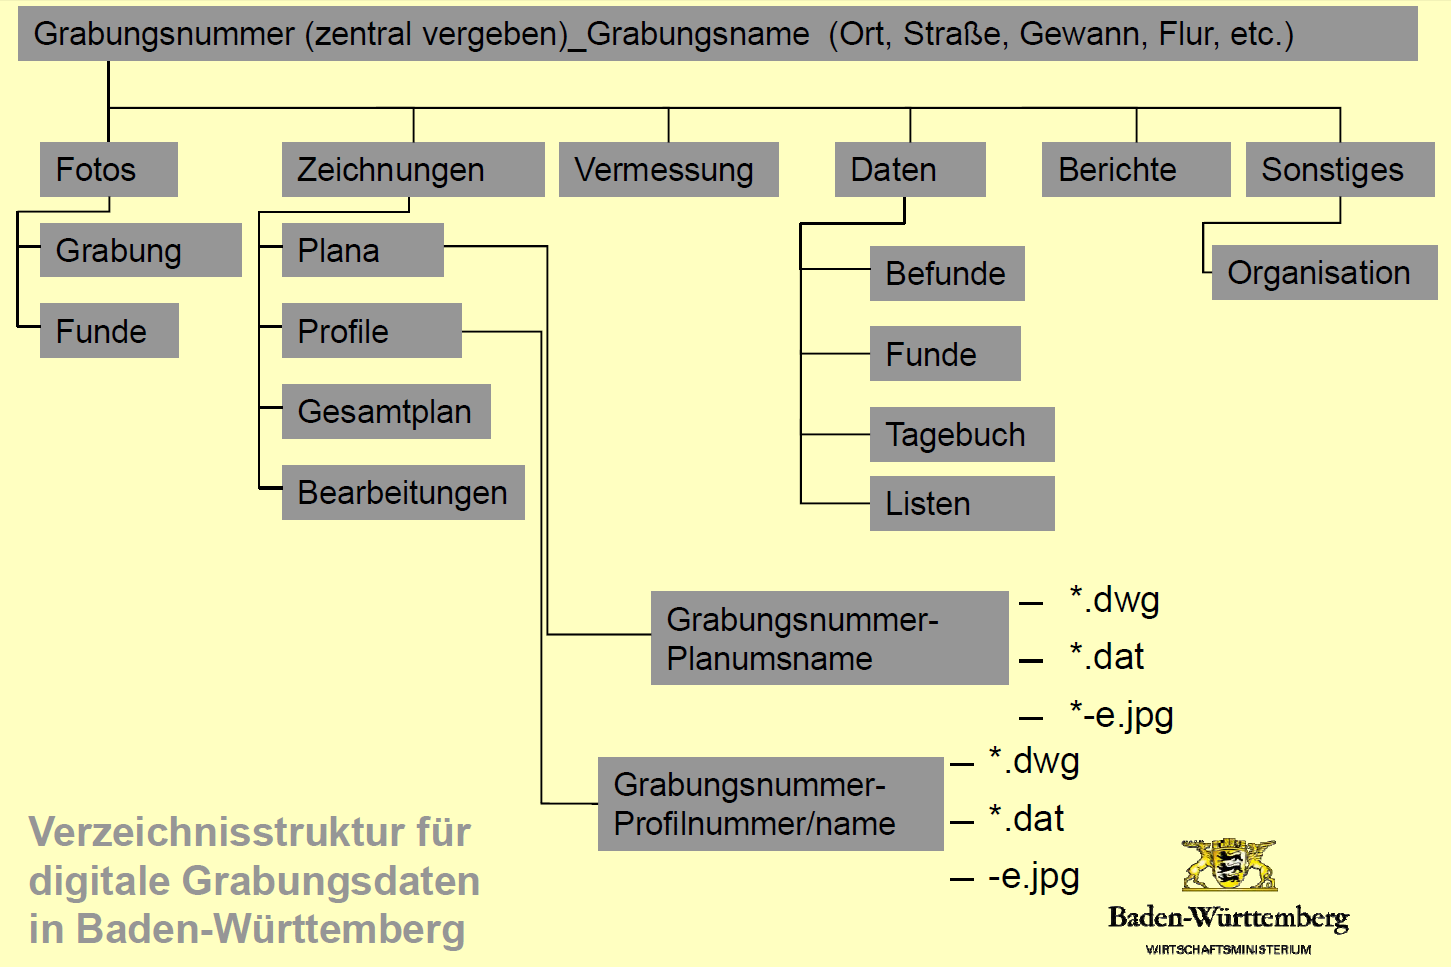
\includegraphics[width=0.9\textwidth]{bilder/OrdnerstrukturBaWue_Bibby}
  \end{center}
  \caption{Datenstruktur Baden-Württemberg}
  \label{OrdnerstrukturBaWue}
\end{figure}

"`\emph{Diese Struktur ist in den oberen Ebenen rigide genug, um für Ordnung und Datendisziplin zu sorgen und gleichzeitig weiter unten flexibel genug, um den unausweichlichen Eigenarten der einzelnen Archäologen Rechnung tragen zu können.}

\emph{Die Grabungs- oder Vorgangsnummer, die zentral vergeben wird, ist wichtig. Sie beschreibt nicht nur die Ausgrabung, sie ist auch die Inventar"=Stammnummer aller Funde, die auf dieser Grabung gefunden werden. Insofern ist sie die Schnittstelle zum zentralen Fundarchiv des Archäologischen Landesmuseums. Die Ausgräber werden aber nicht allein gelassen. Mit der Datenstruktur werden Anleitungen geliefert, die beschreiben, was wohin gehört. Damit wird tatsächlich eine gewisse Einheit im Land erreicht.}"'\footnote{D. Bibby, Digitale Datenstruktur auf Ausgrabungen und Archivierung digitaler Grabungsdaten. Praxis und Praxisversuche aus Baden-Württemberg, ANachr 14 2009, 159-163.}

Auch die nachträgliche Strukturierung von bereits vorhandenen digitalen Dateiablagen ist relativ einfach, da Klartextinhaltsverzeichnisse in der obersten Ebene des Verzeichnisses abgelegt werden können, welche die Eigenheiten der Grabung und die strukturellen Abweichungen beschreiben.

Der Aktenplan des Archäologischen Museums Hamburg wurde für ein analoges Projektarchiv entwickelt, lässt sich jedoch mit wenigen Anpassungen auch gut auf eine digitale Dateiablage anwenden. 

%HAMBURG
\begin{center}
	\begin{longtable}{l l l l}
		\toprule
		\multicolumn{2}{l}{Aktenplan des Archäologischen Museums Hamburg} \\ \midrule \endfirsthead
		\multicolumn{2}{l}{\footnotesize Fortsetzung der vorhergehenden Seite}\\
		\toprule
		\multicolumn{2}{l}{Aktenplan des Archäologischen Museums Hamburg}\\ \midrule \endhead
		\bottomrule \multicolumn{2}{r}{{\footnotesize Fortsetzung auf der nächsten Seite}} \\
		\endfoot
		\bottomrule 
		\endlastfoot
		
		\multicolumn{2}{l}{
\includegraphics[width=0.4cm]{bilder/OrdnerIconZu.png} \hspace*{0.04cm} Datenträger \textit{(nur analog)}}\\
		
		\multicolumn{2}{l}{
\includegraphics[width=0.4cm]{bilder/OrdnerIconAuf.png} \hspace*{0.04cm} Berichte}\\
		& 
\includegraphics[width=0.4cm]{bilder/DateiIcon.png}\hspace*{0.04cm} Grabungsbericht\\
		& 
\includegraphics[width=0.4cm]{bilder/DateiIcon.png} \hspace*{0.04cm} Zwischenberichte\\
		& 
\includegraphics[width=0.4cm]{bilder/DateiIcon.png} \hspace*{0.04cm} Anlagen Zwischenberichte\\
		
		\multicolumn{2}{l}{
\includegraphics[width=0.4cm]{bilder/OrdnerIconAuf.png} \hspace*{0.04cm} Vermessung}\\
	    & 
\includegraphics[width=0.4cm]{bilder/DateiIcon.png} \hspace*{0.04cm} Vermessungspläne\\
		& 
\includegraphics[width=0.4cm]{bilder/DateiIcon.png} \hspace*{0.04cm} Vermessungsunterlagen\\
		& 
\includegraphics[width=0.4cm]{bilder/DateiIcon.png} \hspace*{0.04cm} Vermessungsprotokolle\\
		
		\multicolumn{2}{l}{
\includegraphics[width=0.4cm]{bilder/OrdnerIconAuf.png} \hspace*{0.04cm} Grabungsplänge}\\
	    & 
\includegraphics[width=0.4cm]{bilder/DateiIcon.png} \hspace*{0.04cm} Zeichnungsliste\\
		& 
\includegraphics[width=0.4cm]{bilder/DateiIcon.png} \hspace*{0.04cm} Übersichtpläne\\
		& 
\includegraphics[width=0.4cm]{bilder/DateiIcon.png} \hspace*{0.04cm} Einzelpläne\\
		& 
\includegraphics[width=0.4cm]{bilder/DateiIcon.png} \hspace*{0.04cm} Arbeitspläne\\
		& 
\includegraphics[width=0.4cm]{bilder/DateiIcon.png} \hspace*{0.04cm} Handzeichnungen und Skizzen\\
		
		\multicolumn{2}{l}{
\includegraphics[width=0.4cm]{bilder/OrdnerIconAuf.png} \hspace*{0.04cm} Tagebuch}\\
	    & 
\includegraphics[width=0.4cm]{bilder/DateiIcon.png} \hspace*{0.04cm} Tagebuchausdruck \textit{(oder digitale Datei)}\\
		& 
\includegraphics[width=0.4cm]{bilder/DateiIcon.png} \hspace*{0.04cm} Notizen\\
		
		\multicolumn{2}{l}{
\includegraphics[width=0.4cm]{bilder/OrdnerIconAuf.png} \hspace*{0.04cm} Befunddokumentation}\\
	    & 
\includegraphics[width=0.4cm]{bilder/DateiIcon.png} \hspace*{0.04cm} Befundliste\\
		& 
\includegraphics[width=0.4cm]{bilder/DateiIcon.png} \hspace*{0.04cm} Befundkatalog\\
		& 
\includegraphics[width=0.4cm]{bilder/DateiIcon.png} \hspace*{0.04cm} Notizen\\
		
		\multicolumn{2}{l}{
\includegraphics[width=0.4cm]{bilder/OrdnerIconAuf.png} \hspace*{0.04cm} Funddokumentation}\\
	    & 
\includegraphics[width=0.4cm]{bilder/DateiIcon.png} \hspace*{0.04cm} Fundliste\\
		& 
\includegraphics[width=0.4cm]{bilder/DateiIcon.png} \hspace*{0.04cm} Inventarliste\\
		& 
\includegraphics[width=0.4cm]{bilder/DateiIcon.png} \hspace*{0.04cm} Schriftwechsel\\
		
		\multicolumn{2}{l}{
\includegraphics[width=0.4cm]{bilder/OrdnerIconAuf.png} \hspace*{0.04cm} Probendokumentation}\\
	    & 
\includegraphics[width=0.4cm]{bilder/DateiIcon.png} \hspace*{0.04cm} Probenliste\\
		& 
\includegraphics[width=0.4cm]{bilder/DateiIcon.png} \hspace*{0.04cm} Schriftwechsel\\
		
		\multicolumn{2}{l}{
\includegraphics[width=0.4cm]{bilder/OrdnerIconAuf.png} \hspace*{0.04cm} Fotodokumentation}\\
	    & 
\includegraphics[width=0.4cm]{bilder/DateiIcon.png} \hspace*{0.04cm} Fotoliste\\
		& 
\includegraphics[width=0.4cm]{bilder/DateiIcon.png} \hspace*{0.04cm} Miniaturausdruck \textit{(oder originale Dateien)}\\
		
		\multicolumn{2}{l}{
\includegraphics[width=0.4cm]{bilder/OrdnerIconAuf.png} \hspace*{0.04cm} Dokumente}\\
	    & 
\includegraphics[width=0.4cm]{bilder/DateiIcon.png} \hspace*{0.04cm} Pläne\\
		& 
\includegraphics[width=0.4cm]{bilder/DateiIcon.png} \hspace*{0.04cm} Dokumente und Texte\\
		& 
\includegraphics[width=0.4cm]{bilder/DateiIcon.png} \hspace*{0.04cm} Schriftwechsel\\
		& 
\includegraphics[width=0.4cm]{bilder/DateiIcon.png} \hspace*{0.04cm} Pressespiegel\\
		\bottomrule
	\end{longtable}
\end{center}

Das Bundesdenkmalamt in Österreich hat in seinen Richtlinien eine verpflichtende Ordnerstruktur veröffentlicht, die in einem übergeordneten Ordner mit der Kennung und Benennung der Maßnahme abgelegt wird. Bemerkenswert an dieser Ordnerstruktur ist die sehr flache Hierarchie ohne verschachtelte Ordner, die ein Hinzufügen weiterer benötigter Ordner in der gleichen Ebene zulässt. 

Für die Dateien 01-03 sind in den Richtlinien detaillierte Angaben über den erwarteten Inhalt zu finden. Dies gilt in etwas geringerem Umfang für die übrigen Ordner.  
%ÖSTERREICH
\begin{center}
	\begin{longtable}{l}
		\toprule
		Ordnerstruktur des Bundesdenkmalamtes Österreich \\ \midrule \endfirsthead
		\footnotesize Fortsetzung der vorhergehenden Seite\\
		\toprule
		Ordnerstruktur des Bundesdenkmalamtes Österreich \\ \midrule \endhead
		\bottomrule \multicolumn{1}{r}{{\footnotesize Fortsetzung auf der nächsten Seite}} \\
		\endfoot
		\bottomrule 
		\endlastfoot
		
		
\includegraphics[width=0.4cm]{bilder/DateiIcon.png} \hspace*{0.04cm} 01 Deckblatt\\
		
\includegraphics[width=0.4cm]{bilder/DateiIcon.png} \hspace*{0.04cm} 02 Bericht -- Teil A\\
		
\includegraphics[width=0.4cm]{bilder/DateiIcon.png} \hspace*{0.04cm} 03 Bericht -- Teil B\\
		
\includegraphics[width=0.4cm]{bilder/OrdnerIconZu.png} \hspace*{0.04cm} 04 Technische Daten\\
		
\includegraphics[width=0.4cm]{bilder/OrdnerIconZu.png} \hspace*{0.04cm} 05 SE-Liste \textit{(Liste der Stratigrafischen Einheiten)}\\
		\includegraphics[width=0.4cm]{bilder/OrdnerIconZu.png} \hspace*{0.04cm} 06 SE-Protokollblätter\\
		\includegraphics[width=0.4cm]{bilder/OrdnerIconZu.png} \hspace*{0.04cm} 07 Objektlisten\\
		\includegraphics[width=0.4cm]{bilder/OrdnerIconZu.png} \hspace*{0.04cm} 08 Objektgruppenlisten \emph{(fakultativ)}\\
		\includegraphics[width=0.4cm]{bilder/OrdnerIconZu.png} \hspace*{0.04cm} 09 Planliste\\
		\includegraphics[width=0.4cm]{bilder/OrdnerIconZu.png} \hspace*{0.04cm} 10 Fundliste\\
		\includegraphics[width=0.4cm]{bilder/OrdnerIconZu.png} \hspace*{0.04cm} 11 Grabungs- bzw. Prospektionsprotokoll\\
		\includegraphics[width=0.4cm]{bilder/OrdnerIconZu.png} \hspace*{0.04cm} 12 Vermessungsunterlagen\\
		\includegraphics[width=0.4cm]{bilder/OrdnerIconZu.png} \hspace*{0.04cm} 13 Originalmessdaten und/oder Metadaten Prospektion\\
		\includegraphics[width=0.4cm]{bilder/OrdnerIconZu.png} \hspace*{0.04cm} 14 Maßnahmenpolygon\\
		\includegraphics[width=0.4cm]{bilder/OrdnerIconZu.png} \hspace*{0.04cm} 15 Technischer Gesamtplan\\
		\includegraphics[width=0.4cm]{bilder/OrdnerIconZu.png} \hspace*{0.04cm} 16 Detailpläne\\
		\includegraphics[width=0.4cm]{bilder/OrdnerIconZu.png} \hspace*{0.04cm} 17 Fotodokumentation\\
		\includegraphics[width=0.4cm]{bilder/OrdnerIconZu.png} \hspace*{0.04cm} 18 Matrix\\
		\includegraphics[width=0.4cm]{bilder/OrdnerIconZu.png} \hspace*{0.04cm} 19 Konservatorische Maßnahmen\\
		\includegraphics[width=0.4cm]{bilder/OrdnerIconZu.png} \hspace*{0.04cm} 20 Sonstige Daten\\
		
		\bottomrule
	\end{longtable}
\end{center}


\hyphenation{
Schnitt-stel-le
}
\label{dateibenennung}
\subsection{Dateibenennung}
Üblicherweise besteht der Dateiname einer Datei aus dem eigentlichen Namen und der durch einen Punkt getrennten Dateinamenserweiterung, die das Format der Datei angibt. Die Erweiterung wird in der Regel von dem Programm, mit dem die Datei gespeichert wurde, automatisch an den Dateinamen gehängt.

Ein Beispiel: \emph{IT-Empfehlungen.pdf} gibt an, dass es sich um eine Datei mit dem Namen \emph{"`IT-Empfehlungen"'} handelt, die in dem PDF-Format vorliegt.

Da die Erweiterung automatisch erzeugt wird, muss die Datei mit einem geeigneten Programm konvertiert werden, wenn man das Dateiformat ändern möchte. In dem Kapitel "`Dateiformate"' ab Seite \pageref{dateiformate} sind ausführliche Informationen darüber zu finden.

Im Folgenden geht es nur noch um den reinen Dateinamen, ohne die Dateinamenserweiterung.

\subparagraph{Erlaubte Zeichen} Moderne Betriebssysteme können mit Sonderzeichen umgehen, zu denen Umlaute und Leerzeichen gehören. Das war aber nicht immer so und kann auch heute noch zu Problemen führen. Webserver lesen zum Beispiel das Leerzeichen als die Zeichenfolge "`$\%20$"' ein und da Umlaute nicht immer gleich kodiert werden, kann auch das zu Schwierigkeiten führen. 

Für die Langzeitarchivierung sollten also nur die alphanumerischen Zeichen des englischen Alphabets, also a-z, A-Z und 0-9 verwendet werden. Zusätzlich kann der Bindestrich ({\bfseries -}) und bei Bedarf auch der Unterstrich ({\bfseries\_}) verwendet werden.

\subparagraph{Zu vermeidende Zeichen} Es gibt eine ganze Reihe von Zeichen, die für besondere Aufgaben von Betriebssystemen verwendet werden. Der Punkt dient zur Trennung des Dateinamens von der Dateinamenserweiterung und der Schrägstrich dient in Windows um Ordnerebenen zu kennzeichnen.

Zu den Zeichen, die absolut nicht verwendet werden dürfen, gehören:
\begin{center}
	\Large \bfseries \textbackslash	 / : * ? "'	< >	|
\end{center}

Die Verwendung von allen weiteren Sonderzeichen ist zwar möglich, kann jedoch zu einem unerwarteten Verhalten des Systems führen. Daher wird von der Verwendung von Leerzeichen und Sonderzeichen, Bindestrich ({\bfseries -}) und Unterstrich ({\bfseries\_}) ausgenommen, abgeraten.

\subparagraph{Groß- und Kleinschreibung} Die Groß- und Kleinschreibung in einem Dateinamen wird von unterschiedlichen Systemen verschieden gedeutet. In Windows beispielsweise kann, wenn es eine Datei mit dem Namen \emph{"`TestDatei"'} schon gibt, keine Datei mit dem Namen \emph{"`testdatei"'} angelegt werden. Andere Systeme könnten dies jedoch erlauben, was aber nicht bedeutet, dass man dies auch tun sollte.

Hat man sich in der Praxis einmal für eine Schreibweise entschieden, muss diese auch konsequent eingehalten werden und insbesondere bei der Arbeit auf verschiedenen Systemen darauf geachtet werden.

\subparagraph{Länge} Der Dateiname sollte so kurz wie möglich und so lang wie nötig sein. Eine aktuelle Obergrenze, die auf manchen Systemen nicht überschritten werden darf, sind 260 Zeichen, wobei dabei der gesamte Dateipfad gezählt wird. Kryptische oder untypische Kürzel sollten vermieden werden, da sie in der Regel in Vergessenheit geraten.

\subsection{Versionskontrolle}\label{versionskontrolle}
Wenn unterschiedliche Personen an einer Datei arbeiten, ist es wichtig, die verschiedenen Änderungen und Entwicklungsstadien zu verfolgen und zu kennzeichnen. Nur so kann vermieden werden, dass an der falschen Dateiversion gearbeitet wird oder diese gar gelöscht wird. Dateiversionen, die nicht mehr benötigt werden, sollten bei Bedarf gelöscht werden.

Es gibt mehrere Strategien, um die Versionskontrolle durchzuführen, die im Folgenden erläutert werden.

\subparagraph{Angabe im Dateinamen} Eine einfache und übersichtliche Methode ist, die Versionsangabe in den Dateinamen zu integrieren. Das kann beispielsweise mit einer Datumsangabe oder Ziffern erfolgen. Durch ein vorangestelltes {\bfseries v} werden die Ziffern als eine Versionsnummer gekennzeichnet, wie zum Beispiel {\bfseries v001}. Führende Nullen stellen sicher, dass die Versionsnummern einheitlich und leichter lesbar sind und richtig sortiert werden.

Eine Kennzeichnung von Versionen durch Worte wie \emph{"`neu"'}, \emph{"`neuer"'} und \emph{"`alt"'} ist unbedingt zu vermeiden. Eine Ausnahme können endgültige Dateiversionen bilden, die der Übersicht halber etwa durch \emph{FINAL} am Ende gekennzeichnet werden können. Es darf aber nur eine Datei mit dieser Kennzeichnung in einem Ordner und einem bestimmten Format vorliegen. Eine endgültige Version, die zum Beispiel sowohl als \emph{docx} als auch als \emph{pdf} vorliegt, ist also erlaubt.

\subparagraph{Angabe in der Datei} Angaben zum Erstellungsdatum und den verschiedenen Versionen und deren Änderungen können im Header der Datei oder in standardisierten Kopfzeilen in der Datei selbst angegeben werden. Bei Textdokumenten bietet sich die Möglichkeit einen Innentitel mit einer Versionshistorie zu verwenden. Ein Beispiel für solch einen Innentitel findet sich am Anfang der PDF-Version dieser Empfehlungen.

\subparagraph{Änderungsprotokoll} Statt einzelne Dateiversionen abzuspeichern, kann auch ein Änderungsprotokoll geführt werden. Dabei werden die einzelnen Änderungen in einer einfachen Textdatei protokolliert, die zusammen mit der eigentlichen Datei abgelegt wird. Im Englischen wird dafür der Begriff \emph{ChangeLog} verwendet.

\subparagraph{Software} Die bisher beschriebenen Methoden sind hauptsächlich manuell anzuwendende Vorgänge. Es gibt jedoch auch Software zur Versionsverwaltung. Deren Einsatz lohnt sich vor allem in großen Projekten, die zentral auf einem Server abgelegt werden. Versionsverwaltungssoftware kann aus den Dateiänderungen automatisch \emph{ChangeLogs} erstellen. Die am weitesten verbreiteten Systeme zur Versionsverwaltung sind \href{http://subversion.apache.org/}{Subversion (SVN)} und \href{https://git-scm.com/}{Git}. Primär wurden sie für die Bedürfnisse von Softwareentwicklern konzipiert, jedoch eignen sie sich auch für allgemeinere Aufgaben. Für die einzelnen Computerarbeitsplätze werden Clients wie \href{https://tortoisesvn.net/}{TortoiseSVN} für SVN oder \href{https://windows.github.com/}{GitHub} für Git benötigt.

Eine einfache Versionsverwaltung für Dateien bieten \href{https://owncloud.org/}{ownCloud}, \href{https://www.dropbox.com/}{Dropbox} und \href{https://drive.google.com/drive/}{Google Drive} wobei die Menge der unterschiedlichen gespeicherten Versionen abhängig von dem persönlichen Speicherplatz ist.

\begin{flushleft}
Git: \urllist{https://git-scm.com/}
Clients für Git: \urllist{https://git-scm.com/downloads/guis}
Subversion (SVN): \urllist{http://subversion.apache.org/}
TortoiseSVN: \urllist{https://tortoisesvn.net/}
ownCloud: \urllist{https://owncloud.org/}
Dropbox: \urllist{https://www.dropbox.com/}
Google Drive: \urllist{https://drive.google.com/drive/}
Vergleich von Versionsverwaltungssystemen auf Wikipedia: \urllist{https://en.wikipedia.org/wiki/Comparison_of_revision_control_software}
\end{flushleft}

\newpage
\section{Dateispeicherung und -sicherung}\label{dateispeicherung}
\abschnittsautor{M. Trognitz, R. Komp, R. Förtsch}
Um Datenverlust vorzubeugen, ist es unerlässlich eine geeignete Sicherungsstrategie zu verwenden. Dabei muss zwischen einer kurzfristigen Speicherung und einer mittelfristigen Sicherung unterschieden werden. Ersteres meint, wie Daten während der Erstellung und Bearbeitung gespeichert werden. Letzteres bezieht sich auf einen längeren Speicherzeitraum, der durchaus auch mehrere Monate betragen kann, stellt also ein klassisches Backup der Daten dar.

Die Sicherungsstrategie legt fest, wie die Datensicherung erfolgen soll und berücksichtigt folgende Fragen:
\begin{itemize}
	\item Wer ist für die Datensicherung verantwortlich?
	\item Wer hat Zugriff auf die gesicherten Daten?
	\item Wann und wie oft soll die Datensicherung durchgeführt werden?
	\item Auf welche Weise soll gesichert werden?
	\item Welche Daten sollen gesichert werden?
	\item Welche Speichermedien sollen verwendet werden?
	\item Wie viele Sicherungskopien sollen angelegt werden?
	\item Wo sollen die Sicherungen aufbewahrt und wie sollen sie geschützt werden?
	\item Wie soll der Transport der Sicherungskopien erfolgen?
	\item Wie lange soll eine Sicherung aufbewahrt werden?
\end{itemize}

Die Sicherungsstrategie kann mit den zu verwendenden Richtlinien zur Dateiablage eng verzahnt sein, um etwa einen nahezu automatisierten Sicherungsvorgang zu ermöglichen.

Die richtige Speicherstrategie beugt zwar möglichen Datenverlusten durch Hardware-, Software- oder menschliche Fehler vor, stellt aber noch \emph{keine} Archivierung der Daten dar. Eine Archivierung ist auf Langfristigkeit ausgelegt und impliziert immer eine bewusste Auswahl und umfassende Dokumentation der Daten, da eine Nachnutzung derselben das Ziel ist. Während der Projektlaufzeit kann bereits ein eigener Archivordner angelegt werden, worin beispielsweise finale Dateien oder unprozessierte Rohdaten abgelegt werden können, um die spätere Auswahl der zu archivierenden Daten vorzubereiten und zu vereinfachen.

Weiterführende Hinweise zur Datensicherung sind auf den Seiten des Bundesamtes für Sicherheit in der Informationstechnik zu finden, die sich sowohl an Einsteiger\footnote{\url{https://www.bsi-fuer-buerger.de/BSIFB/DE/MeinPC/Datensicherung/Sicherungsmethoden/sicherungsmethoden\_node.html}} als auch an Experten\footnote{\url{https://www.bsi.bund.de/DE/Themen/ITGrundschutz/ITGrundschutzKataloge/Inhalt/\_content/baust/b01/b01004.html}} richten. 
\subsection{Kurzfristige Speicherung}
Zur Bearbeitung geöffnete Dateien sollten in kürzeren Abständen gespeichert werden, um einem Verlust von stundenlanger Arbeit infolge etwa eines Stromausfalls vorzubeugen. Von diesen Arbeitsversionen sollten regelmäßig, beispielsweise nach jedem Arbeitstag, Kopien auf externen Speichermedien angefertigt werden, welche in die mittelfristige Sicherung übergehen.

Vorgaben zur Form der Dateiablage, der Dateibenennung und Versionierung müssen schon beim Anlegen der Dateien beachtet werden, um einen reibungslosen Ablauf der darauf abgestimmten Datensicherungsstrategie zu gewährleisten. Hinweise dazu sind im Abschnitt Dateiverwaltung ab Seite \pageref{dateiverwaltung} zu finden.

\subsection{Mittelfristige Sicherung}
Digitale Daten sind nur dann über einen längeren Zeitraum sicher, wenn sie mehr als einmal gespeichert werden. Es müssen also mindestens zwei Sicherungskopien auf physisch getrennten Speichermedien vorliegen, um etwa bei einem Hardwaredefekt auf eine alternative Sicherungskopie zugreifen zu können.

Die Sicherung von Daten auf unterschiedlichen Arbeitsgeräten wird erleichtert, wenn diese zunächst auf einem Datenträger gesammelt werden und dieser dann gesichert wird.

\subparagraph{Speichermedium} Welches Speichermedium gewählt wird, hängt vor allem von der Speichergröße der zu sichernden Dateien und der vorhandenen Infrastruktur ab. So eignen sich eine CD oder eine DVD nur für Daten bis maximal 900 MB bzw. 17 GB Speichervolumen. Für größere Datenmengen werden entsprechend größere Datenträger benötigt. 

Steht ein lokaler oder institutioneller Server zur Verfügung, sollte dieser zur Datensicherung verwendet werden, da diese üblicherweise gewartet werden und meist selbst in eigene Sicherungsstrategien eingebunden sind. In Umgebungen mit Zugriff auf das Internet, kann eine Sicherung auch auf einen entfernten Server, beispielsweise in einem Rechenzentrum, erfolgen. In allen anderen Fällen können externe Festplatten verwendet werden. Von externen kommerziellen Diensten, wie beispielsweise Dropbox, ist für eine mittelfristige Sicherung abzuraten, weil es sich oft um ausländische Anbieter handelt, die nicht dem deutschen Recht unterliegen und den Nutzer im Unklaren darüber lassen, wie mit den Daten umgegangen wird.

Da die Speichermedien eine begrenzte Lebenszeit von etwa zehn Jahren haben, sollten die Sicherungen von Zeit zu Zeit auf neue Speichermedien migriert werden. Außerdem sollten sie zwischenzeitlich an verschiedenen Orten, mindestens in verschiedenen Räumen, gelagert werden, um etwa im Brandfall den Schaden zu begrenzen. Auch der Transport von Original- und Sicherungsdatenbeständen sollte getrennt durch unterschiedliche Personen erfolgen, um zu vermeiden, dass etwa durch Diebstahl alle Sicherungskopien auf einmal abhanden kommen. 

Für das Kopieren der Daten auf ein Speichermedium gibt es verschiedene Methoden, wie die im Folgenden beschriebene Volldatensicherung, inkrementelle und differentielle Datensicherung.

\subparagraph{Volldatensicherung} Bei der Volldatensicherung werden die zu sichernden Dateien komplett und eins zu eins auf ein Speichermedium kopiert. Wird zum ersten Mal eine Sicherungskopie angelegt, so muss dies als Volldatensicherung geschehen. Dabei ist zu beachten, dass der Kopiervorgang viel Zeit in Anspruch nehmen kann, wobei dies auch über Nacht geschehen kann. Vor der Ausführung der Volldatensicherung muss geprüft werden, dass auf dem Speichermedium ausreichend freier Speicherplatz vorhanden ist. 

Die Volldatensicherung ist die einzige Methode, die manuell, ohne weitere Hilfsprogramme, durchgeführt werden kann. Wird eine Volldatensicherung angelegt, sollten, beispielsweise in einer Textdatei, Informationen gespeichert werden, die Auskunft über den Zeitpunkt der Sicherung, den Ansprechpartner und den Umfang der Daten geben.

Liegt eine erste Volldatensicherung vor, können neue oder geänderte Daten mittels inkrementeller oder differentieller Datensicherung gesichert werden, was die Möglichkeit bietet, verschiedene Versionen der Daten zu sichern. Für beide Methoden werden jedoch eigene Programme benötigt.

\subparagraph{Inkrementelle Sicherung} Die inkrementelle Sicherung speichert nur jene Daten, die sich im Vergleich zu der vorliegenden Volldatensicherung oder vergangenen inkrementellen Sicherungsvorgängen geändert haben. Dies spart Zeit und Speicherplatz, erfordert jedoch im Fall einer Wiederherstellung der Daten, dass zunächst die Volldatensicherung übertragen wird und anschließend alle erfolgten inkrementellen Sicherungen nacheinander eingespielt werden.

\subparagraph{Differentielle Sicherung} Bei der differentiellen Sicherung werden immer jene Daten gespeichert, die sich im Verlgeich zu der vorliegenden letzten Volldatensicherung geändert haben. Im Unterschied zu der inkrementellen Sicherung entfällt also der Vergleich mit Daten aus zwischenliegenden Sicherungsvorgängen seit Erstellung der Volldatensicherung. Diese Methode erfordert zwar etwas mehr Zeit und Speicherplatz als die inkrementelle Sicherung, erleichtert aber die Wiederherstellung der Daten, da nur die Volldatensicherung und die letzte differentielle Sicherung auf das System übertragen werden muss. Die vorherigen differentiellen Sicherungen werden nicht benötigt.

\subparagraph{Automatisierung} Die Datensicherung kann mit Hilfe von Programmen oder Skripten automatisiert erfolgen. Wichtig ist dabei zu kontrollieren, dass die Datensicherung auch tätsächlich in der gewünschten Form ausgeführt wird. Geeignete Programme gibt es viele, wie beispielsweise \href{http://bacula.org/}{Bacula}, \href{http://www.dirsyncpro.org/}{DirSync Pro}, \href{http://www.traybackup.de}{TrayBackup}, \href{http://personal-backup.rathlev-home.de}{PersonalBackup} oder \href{http://rsync.samba.org/}{rsync}. Eine ausführliche Liste ist außerdem auf der englischen Wikipedia unter \href{http://en.wikipedia.org/wiki/List\_of\_backup\_software}{List of backup software} zu finden. Oft können die Programme auch zur Wiederherstellung von gesicherten Daten verwendet werden.

\begin{flushleft}
	DirSync Pro: \urllist{http://www.dirsyncpro.org/}
	TrayBackup: \urllist{http://www.traybackup.de}
	PersonalBackup: \urllist{http://personal-backup.rathlev-home.de}
	rsync: \urllist{http://rsync.samba.org/}
	Liste von Backup-Programmen auf Wikipedia: \urllist{http://en.wikipedia.org/wiki/List_of_backup_software} 
\end{flushleft}

\subparagraph{Sicherungszeitpunkt} Der Zeitpunkt der Sicherung spielt eine nicht zu unterschätzende Rolle. Beispielsweise kann eine Sicherung von Datenbanken im laufenden Betrieb zu Inkonsistenzen führen, weshalb in solchen Fällen ein Administrator diese Aufgabe übernehmen sollte.

Regelmäßige Sicherungsvorgänge, die zu bestimmten Zeitpunkten täglich, wöchentlich oder monatlich automatisiert gestartet und durchlaufen werden, gewährleisten, dass eine Sicherung auch tatsächlich erfolgt, zumal sie nicht vom individuellen Verhalten eines Nutzers abhängen.

Für Daten, die verschiedene Arbeitsschritte durchlaufen und dadurch große Änderungen erfahren, können die verschiedenen Zustände als Sicherungspunkte gespeichert werden. Beispielsweise können zunächst unbearbeitete digitale Bilder gespeichert werden, sowie ein daraus erzeugtes photogrammetrisches Modell oder andere nicht oder nur schwer reproduzierbare signifikante Verarbeitungsschritte. Solche Sicherungspunkte müssen allerdings manuell gemacht werden, indem beispielsweise ein Ordner mit den Rohdaten angelegt wird. Hinweise für solche Sicherungspunkte werden für bestimmte angewendete Methoden in dem Kapitel Forschungsmethoden ab Seite \pageref{methoden} gegeben.

\subparagraph{Sicherungsversionen} Es empfiehlt sich, eine vorhandene Volldatensicherung nicht direkt mit einer neuen Volldatensicherung zu überschreiben. Tritt nämlich während des Sicherungsvorganges ein Fehler auf, könnte auch die bereits vorhandene Sicherungsversion beschädigt werden.

Bei der Anwendung von inkrementellen oder differentiellen Sicherungsmethoden sollte trotzdem in geregelten Zeitabständen eine neue Volldatensicherung angelegt werden, welche mindestens bis zur nächsten Volldatensicherung aufgehoben wird. Dies ist im Sinne des Generationenprinzips oder Großvater-Vater-Sohn-Prinzips, einer Strategie zur Datensicherung, bei der mehrere Sicherungen für verschiedenen Zeitpunkte und Zwecke angelegt werden. Hierfür können beispielsweise wöchentlich und monatlich Volldatensicherungen angelegt werden (Vater und Großvater), die primär den Datenverlust durch Hardware- oder Software-Fehler reduzieren sollen. Tägliche inkrementelle oder differentielle Sicherungen (Sohn) erlauben es beispielsweise auf Arbeitsversionen des Vortages zuzugreifen und können mit dem Beginn einer neuen Woche nach und nach überschrieben werden. 

\subparagraph{Disaster Recovery} Eine gute Sicherungsstrategie umfasst zusätzlich die Erprobung der Wiederherstellung der Daten, um im Ernstfall sicher zu sein, dass die verwendete Strategie auch wirklich funktioniert und die Daten schnell wieder einsatzfähig sind. Somit können vorhandene Sicherungsversionen ebenfalls auf ihre Funktionsfähigkeit überprüft werden.

\chapter{Dateiformate}
Unterscheidung zwischen Einzeldateien (Datentypen) (einzelne atomare Dateien) und Datensets (zusammenhängende Dateien, wie etwa eine Datenbank, die ja aus mehreren Tabellen besteht). 

	\section{Einfache Dateiformate}
\subsection{Textdokumente}

\subsubsection{Finale Version}
\subsubsection{Editierbarer Text}
\subsubsection{Reiner Text}
\subsubsection{Strukturierter Text}

\subsection{Präsentationen}

\subsection{Tabellen}

\subsection{Statische Bilder}

Mit statischen Bildern sind alle unbewegten digitalen Bilder gemeint, die entweder direkt digital erzeugt wurden oder Digitalisate von analogen Quellen darstellen.
Grundsätzlich wird unterschieden zwischen Rastergrafiken, die aus einzelnen Bildpunkten, den Pixeln, zusammengesetzt sind, und Vektorgrafiken, die mit grafischen Primitiven, z.B. Linien, beschrieben werden. Dementsprechend werden unterschiedliche Mindeststandards beschrieben.

Bilder einer Digitalkamera sind immer Rastergrafiken. Vektorgrafiken sind beispielsweise mit Hilfe von CAD-Programmen erzeugte Pläne. Im Gegensatz zu Rastergrafiken sind Vektorgrafiken ohne Qualitätsverlust beliebig skalierbar.

\subsubsection{Rastergrafiken}

Bei Rastergrafiken, auch Pixelgrafiken, handelt es sich um digitale Bilder, die mittels rasterförmig angeordneter Pixel beschrieben werden. Jedem Pixel ist dabei ein Farbwert zugeordnet. Rastergrafiken haben eine fixe Größe.

Zu den Rastergrafiken gehören: Digitale Fotografien jeder Art, Satellitenbilder, digitalisierte Bilder (Scans), Screenshots sowie digitale Originalbilder und -grafiken.

\paragraph{Übersicht}

%\begin{center}
%	\begin{tabular}{c l p{0.4\textwidth}}
%		\toprule
%		\multicolumn{2}{l}{Format} & Minimaldokumentation \\ \midrule
%		\multirow{3}{*}{\color{ForestGreen} \LARGE \checkmark} & Baseline TIFF, unkomprimiert & \multirow{8}{0.4\textwidth}{Identifikator\\ 
%																																																												Bildunterschrift\\ 
%																																																												Beschreibung\\ 
%																																																												Urheber\\ 
%																																																												Datum\\ 
%																																																												Rechte\\ 
%																																																												Schlagworte\\ 
%																																																												Ort}\\
%  	& DNG &  \\
% 		& Geo-Tiff &  \\ \cmidrule(r){1-2}
% 		\multirow{1}{*}{$\color{BurntOrange} \scriptstyle \thicksim$} & PNG &  \\
% 		& &  \\
% 		& &  \\
% 		& &  \\
% 		& &  \\
%		\bottomrule    
%	\end{tabular}
%\end{center}

\subparagraph{Format} Alle als Rastergrafiken\index{Rastergrafik} vorliegenden Roh- und Urfassungen (Master) von Bildern sind in angemessener Qualität und unkomprimiert im baseline TIFF- oder DNG-Format abzuspeichern. Für georeferenziertes digitales Bildmaterial ist zwecks Erhalt der Referenzdaten das Geo-Tiff-Format zu verwenden.

Nur für Grafiken, \emph{nicht} für Fotos, eignet sich auch das PNG-Format. Allerdings ist jederzeit das TIFF-Format vorzuziehen. JPEG, bzw. JPG, eignet sich nicht zur Langzeitarchivierung, da es keine verlustfreie Komprimierung anbietet.

Es muss darauf geachtet werden, dass die Bildgröße und -auflösung der originalen Datei erhalten bleibt, wenn in andere Formate umgewandelt wird. Außerdem muss bei der Konvertierung darauf geachtet werden, dass eine verlustfreie Komprimierung verwendet wird. Auch Farbtiefe und Farbraum sollten nach der Konvertierung erhalten bleiben.

Bilder, die Ebenen enthalten, müssen vorher auf eine Ebene reduziert werden. Bei Bedarf, sollten die verschiedenen Ebenen und Komponenten als einzelne Dateien abgespeichert werden. 

%\begin{center}
%	\fboxrule0.5mm
% 	\fcolorbox{ianusGrau}{white}{\parbox[c]{0.95\textwidth}{{\scshape\large\color{ianusBlau}Achtung} Wiederholtes Bearbeiten und Abspeichern, führt zu einer allmählichen Abnahme der Qualität. Dieser sogenannte \gls{Generationsverlust} tritt insbesondere bei der verlustbehafteten Bildkomprimierung auf.}}
%\end{center}

Hinweis: Wiederholtes Bearbeiten und Abspeichern, führt zu einer allmählichen Abnahme der Qualität. Dieser sogenannte Generationsverlust tritt insbesondere bei der verlustbehafteten Bildkomprimierung auf.

\begin{center}
	\begin{tabular}{l p{0.2\textwidth} p{0.6\textwidth}}
		\toprule
		\multicolumn{2}{l}{Format} & Begründung \\ \midrule
		\multirow{3}{*}{\color{ForestGreen} \LARGE \checkmark} & Baseline TIFF, unkomprimiert & TIFF ist quasi ein Standardformat für die digitale Langzeitarchivierung von Bilddateien und unterstützt auch die Speicherung von Metadaten im Exif-Format. Obwohl das Format auch Kompression verwenden kann, kommt für die Langzeitarchivierung nur die unkomprimierte Form in Frage. \\
		  & DNG & Das von Adobe entwickelte Digital Negative Format ist ein offenes Format, das für die Langzeitarchivierung geeignet ist. Damit können RAW-Dateien und deren Metadaten (Exif oder IPTC-NAA) gelesen und gespeichert werden. Außerdem können über XMP weitere Metadaten eingespeist werden.\\ 
		  & Geo-Tiff & Geo-Tiff basiert auf TIFF und ist besonders für georeferenzierte Bilddaten geeignet, da somit die Referenzdaten erhalten bleiben.\\ \cmidrule(r){1-3}
		\multirow{1}{*}{$\color{BurntOrange} \thicksim$} & PNG & PNG ist eine verlustfreie Alternative zu dem GIF-Format, welches eine verlustbehaftete Kompression verwendet. Es bietet eine Farbtiefe von 32 Bit, einen Alphakanal für Transparenz und verlustfreie Kompression. Allerdings wird nur RGB als Farbraum unterstützt und es können keine Exif-Daten gespeichert werden. Das Format eignet sich \emph{nicht} für digitale Fotos. \\ \cmidrule(r){1-3}
		\multirow{2}{*}{\LARGE \boldmath$\color{BrickRed} \times$}& JPEG & Trotz einiger Vorzüge, eignet sich das JPEG-Format \emph{nicht} für die Langzeitarchivierung, da es \emph{keine} verlustfreie Komprimierung bietet.\\
		 & GIF & GIF kann sowohl statische, als auch animierte Bilder speichern. Da es aber verlustbehaftet komprimiert, wird PNG als Alternativformat empfohlen. \\
 		\bottomrule    
	\end{tabular}
\end{center}


\subparagraph{Dokumentation}
\label{Metadaten-Rastergrafiken} Eingebettete Metadaten, wie Exif, IPTC-NAA oder XMP, sollten behalten und archiviert werden. Am besten werden sie in eine eigene Text- oder XML-Datei transferiert und getrennt gespeichert.

Neben technischen Informationen, die sich hauptsächlich mit der Erstellung der Rastergrafik befassen, sollten vor allem auch beschreibende und administrative Metadaten über das Bild gespeichert werden. Die hier angegebenen Metadaten sind als minimale Angabe zu betrachten. Weitere Metadaten sind methodenabhängig und können in den jeweiligen Abschnitten nachgelesen werden.

Hinweis: Werden digitale Aufnahmen mit Programmen bearbeitet, welche die eingebetteten Metadaten ignorieren, gehen diese verloren. 

\begin{center}
	\begin{tabular}{l p{0.6\textwidth}}
		\toprule
		Metadatum & Beschreibung \\ \midrule
		Identifikator & Name der Datei, z.B. grabung01.tif \\
		Bildunterschrift & Der Titel oder eine passende Bildunterschrift des Bildes \\
		Beschreibung & Beschreibung des Bildes  \\
		Urheber & Name des Fotografen oder Erstellers \\
		Datum & Datum der Erstellung oder letzten Änderung des Bildes\\
		Rechte & Details zum Urheberrecht \\
		Schlagworte & Schlagworte, wie z.B. Periode, Fundstelle oder charakteristische Merkmale. Wenn vorhanden, angemessene Thesauri verwenden\\
		Ort & Ortsinformationen zu dem Bild. Möglichst in einem standardisierten Format angeben, wie z.B. Lat/Long oder Schlagworte aus einem geeigneten Thesaurus, z.B. Getty Thesaurus of Geographic Names oder GeoNames \\
		Dateiformat \& Version & z.B. Baseline TIFF 6.0 \\
		Dateigröße & Größe der Datei in Bytes \\
		Bildgröße & Maße des Bildes gemessen in Pixeln, z.B. $400px \times 700px$ \\
		Auflösung & Bildauflösung, gemessen in Punkten pro Zoll (dpi) \\
		Farbraum & Der in dem Bild verwendete Farbraum, z.B. RGB oder Graustufen \\
		Farbtiefe & z.B. 24 bit oder 8 bit \\
		Aufnahmegerät & Beispielsweise Details zur Kamera oder dem Scanner \\
		Software & Software mit der das Bild aufgenommen, erstellt oder bearbeitet wurde, wie z.B. Adobe Photoshop CS3 \\ 
 		\bottomrule    
	\end{tabular}
\end{center}


\paragraph{Vertiefung} ~\\ 

Da eine Rastergrafik mit in einem rechteckigen Raster angeordneten Bildpunkten beschrieben wird und jedem dieser Punkte (Pixel), ein Farbwert zugeordnet wird, gibt es zwei Hauptmerkmale: die Bildgröße und die Farbtiefe. Abhängig von der Bildgröße ist die Auflösung. Hinzu kommen noch weitere Eigenschaften, wie Farbmodell und Farbraum, Komprimierung, Transparenz, Ebenen und Metadaten die hier ausführlicher erklärt werden. 

Die einzelnen Eigenschaften können in Abhängigkeit von Quelle und Verwendung der Grafik stark variieren. Es ist praktisch unmöglich, genaue Vorgaben für die einzelnen Einstellungsmöglichkeiten zu machen. Sie sollten im Kontext des Projektes betrachtet werden und ihren Zweck erfüllen. Nichtsdestotrotz werden in diesem Abschnitt Anmerkungen über die Qualität gemacht.

Entscheidend für die Nachnutzung von Rastergrafiken ist die Dokumentation, worin auch die Entscheidung für ein bestimmtes Format und dessen Einstellungen begründet werden kann.


\subparagraph{Bildgröße und Auflösung}
Die Bildgröße beschreibt den Detaillierungsgrad einer Grafik mittels der Pixelanzahl. Dabei gilt: Je mehr Bildpunkte, desto höher ist auch der Detaillierungsgrad und die Dateigröße. <<XXX Grafik mit Bildchen 1x1; 2x2; 4x4; usw... IANUS Logo>> Die Pixelanzahl kann durch die Gesamtanzahl der Bildpunkte, wie beispielsweise in der Digitalfotografie mittels Megapixeln, oder mit der Anzahl der Bildpunkte je Zeile mal der Anzahl der Bildpunkte je Spalte (z.B. $1024 \times 768$) angegeben werden. Aus der zweiten Darstellungsvariante geht auch das Seitenverhältnis hervor.

Umgangssprachlich wird die Bildgröße auch als Bildauflösung bezeichnet. Allerdings hängt die Auflösung von einem physikalischen Wiedergabemedium (z.B. Bildschirm oder ein A4 Ausdruck) ab, wobei die Punktdichte maßgeblich für die Wiedergabequalität ist. Die Punktdichte wird üblicherweise in Punkten (\emph{dots per inch; dpi}), Pixeln (\emph{pixel per inch; ppi}) oder Linien (\emph{lines per inch; lpi}) pro Zoll (\emph{inch}) angegeben. Soll das Bild nur digital verwendet werden, reicht eine minimale Auflösung von 72dpi aus. Wenn das Bild jedoch gedruckt werden soll, muss mit einer Mindestauflösung von 300dpi gearbeitet werden.

Abhängig von der Aufgabe einer Rastergrafik muss eine geeignete Bildgröße gewählt werden. Dabei sollte bedacht werden, dass die Dateigröße mit dem Detaillierungsgrad steigt, und somit eine Balance zwischen dem benötigtem Detaillierungsgrad und der Dateigröße gefunden werden muss.


\subparagraph{Farbtiefe}

Mit der Farbtiefe (engl. auch \emph{bit depth}) wird die Anzahl der Bits angegeben, die den Farbwert eines Pixels speichern. Ein Bit kann dabei $2^1$, also zwei Farbwerte (z.B. Schwarz und Weiß) speichern. Die Anzahl der darstellbaren Farbwerte steigt mit der Anzahl der Bits exponentiell. So können mit 8 Bits bereits $2^8$ also 256 Farbwerte (üblicherweise Graustufen) und mit 24 Bits schon $2^{24} = 16.777.216$ Farbwerte (\emph{True color}) dargestellt werden. Größere Farbtiefen von 30, 32, 36, 40 und 48 Bit werden hauptsächlich im Scan-, Kino-, TV- und Druckbereich verwendet.

Wie bei der Bildgröße steigt auch hier die Dateigröße mit der Farbtiefe, weshalb nur die minimal notwendige Farbtiefe gewählt werden sollte. Beispielsweise reicht es aus, eine Schwarz-weiß Grafik mit 8-Bit Graustufen zu speichern.

Ein Spezialfall sind indizierte Farben. Dabei wird für ein Pixel nicht direkt der Farbwert, sondern ein Index auf eine Farbe aus einer vorgegebenen Farbtabelle oder Farbpalette gespeichert. Somit können Bilder mit wenigen Farben Speicherplatz einsparen. Beispielsweise bietet das Dateiformat GIF eine Farbtiefe von 8 Bit.


\subparagraph{Farbmodell und Farbraum}

Ein Farbmodell ist ein mathematisches Modell, das üblicherweise mit Hilfe von Zahlentupeln beschreibt wie Farben dargestellt werden können. Alle Farben eines Farbmodells können dreidimensional als Farbraum dargestellt werden.

Übliche Farbmodelle sind RGB und CMYK. RGB wird hauptsächlich für die Bildschirmanzeige verwendet, während CMYK im Druckbereich verwendet wird. Insgesamt enthält RGB mehr Farbkombinationen als CMYK, weshalb es sein kann, dass RGB-Grafiken nicht exakt farbtreu gedruckt werden können. 

Ein Farbmodell kann auf mehrere Farbräume abgebildet werden, weshalb es für RGB unter anderem die Farbräume \emph{sRGB} und \emph{Adobe RGB} gibt. Die eben genannten Farbräume sind genormte, ausreichend große Farbräume, die für die meisten Anwendungen ausreichen.

Die Kombination von Farbtiefe und Farbmodell beschreibt wie viele Bits pro Farbwert zur Speicherung zur Verfügung stehen und wie viele Farben im Endeffekt dargestellt werden. Beispielsweise bietet \emph{True Color} für RGB, mit einer Farbtiefe von 24 Bit, jeweils 8 Bit für Rot, Grün und Blau. Da man bei CMYK noch einen vierten Wert berücksichtigen muss, hat \emph{True Color} für CMYK eine Farbtiefe von 32 Bit.

Wenn man im Zweifel ist, ob RGB oder CMYK verwendet werden soll, ist zu empfehlen das RGB-Farbmodell zu verwenden, da damit mehr Farben abgebildet werden können. Bei Bedarf lässt sich der Farbraum nachträglich in CMYK oder in einen indizierte Farbraum konvertieren.


\subparagraph{Komprimierung}
Das Ziel einer Komprimierung ist, die Dateigröße für einen bestimmten Zweck zu reduzieren, wie etwa zur Darstellung im Internet. Die Komprimierung von Rastergrafiken kann entweder verlustfrei oder verlustbehaftet erfolgen. Grundsätzlich sollte bei der Speicherung, einem Format den Vorzug gegeben werden, das entweder gar keine (z.B. TIFF oder PNG) oder verlustfreie (z.B. GIF, PNG oder TIFF) Komprimierung verwendet. Verlustbehaftete Formate, wie etwa JPEG, sollten nur dann verwendet werden, wenn es nicht anders geht (z.B. weil die verwendete Digitalkamera nur dieses Speicherformat bietet) und möglichst bald in ein verlustfreies Format konvertiert werden.

Im Umgang mit Rastergrafiken ist es wichtig, sich bewusst zu machen, wann eine Komprimierung erfolgt und in welchem Grad dies passiert. So führt etwa häufiges Bearbeiten und Abspeichern von JPEGs zum sogenannten Generationsverlust, der mit der Verwendung von TIFF-Dateien vermieden werden kann.

TIFF bietet die Möglichkeit, eine verlustfreie Komprimierung mit LZW anzuwenden. Allerdings ist dieses komprimierte TIFF-Format noch nicht für die Langzeitarchivierung erprobt.


\subparagraph{Transparenz}

Transparente Elemente in Grafiken werden von vielen Vektorgrafikformaten unterstützt. Doch da Transparenzen üblicherweise mit dem sogenannten Alphakanal gespeichert wird, benötigt man ein Rastergrafikformat, das diesen berücksichtigt, wie z.B. TIFF, PNG oder GIF. 

Bei der Konvertierung von einem Format in ein anderes, sollte darauf geachtet werden, ob Transparenzen auch unterstützt werden.


\subparagraph{Ebenen}
Eine weit verbreitete Funktion von Grafikprogrammen ist die Möglichkeit, verschiedene Bildelemente auf verschiedenen Schichten, den sogenannten Ebenen, zu verteilen. Diese Eigenschaft wird von Rastergrafikformaten nicht unterstützt! 

Wenn man die Datei als Rastergrafik speichert, werden die Ebenen von oben nach unten verschmolzen. Möchte man aber einzelne Ebenen auch für die Zukunft speichern, kann man in Erwägung ziehen, jede Ebene für sich als eigene Bilddatei zu speichern.

\subparagraph{Metadaten}

Einige Bildformate unterstützen die Speicherung der Metadaten direkt in der Datei. Dazu gehören auch TIFF, DNG und JPEG. Es gibt drei gebräuchliche Metadatenformate bzw. -standards, welche die Informationen jeweils in den Header der Bilddatei schreiben. Der erste für professionelle Arbeitsabläufe gestaltete Standard IIM wurde ab 1995 von Adobe teilweise als Metadaten in Photoshop übernommen, wodurch der IPTC-NAA-Standard festgelegt wurde. Gleichzeitig führte Adobe aber auch den XMP-Standard ein. Ein weiterer Standard ist Exif, der vor allem von Digitalkameras zur Speicherung der Aufnahmeinformationen verwendet wird.

Etwas problematisch ist, dass jeder Standard die Informationen in den Header der Bilddatei schreibt, weshalb die Gefahr besteht, dass sie sich teilweise überschreiben. Deshalb wird empfohlen, die Metadaten zu extrahieren und in einer gesonderten Textdatei zu speichern. Was für diese gesonderte Datei beachtet werden muss, wird im allgemeinen Abschnitt über Metadaten, \ref{Metadaten-allgemein}, auf Seite \pageref{Metadaten-allgemein} erläutert.

Die Informationen im Header sollten nicht komplett gelöscht werden, da gespeicherte Metadaten im Dateiformat selbst dazu beitragen verwaiste Werke, die keinerlei Rückschlüsse auf den Urheber zulassen, zu verhindern.

Die Problematik der drei unterschiedlichen Standards wurde auch von namhaften Herstellern erkannt, weshalb die Metadata Working Group gegründet wurde, welche die Verwendung von Metadaten in Bilddateien vereinheitlichen will. Es soll aber nicht ein neuer Standard geschaffen werden, sondern die Nutzung der bestehenden Standards durch einen übergreifenden Rahmen geregelt werden.


\subparagraph{Anmerkungen zur Qualität}
Gerade weil Rastergrafiken ein breites Anwendungsspektrum bieten, können hier keine spezifischen Aussagen zur Qualität gemacht werden. Im Prinzip muss also der Ersteller entscheiden, was für die jeweilige Aufgabe angemessen ist. Dabei sollte aber nicht nur auf die aktuellen konkreten Anforderungen, sondern gerade im Hinblick auf die spätere Verwendung (z.B. Publikation) oder Arbeitsschritte (z.B. Konvertierung) auch auf zukünftige Anforderungen geachtet werden.

Eine große Datei ist nicht gleichbedeutend mit guter Qualität. Andererseits sollte auch nicht zugunsten von Speicherplatz auf die Qualität verzichtet werden.


\paragraph{Praxis} ~\\

In diesem Abschnitt sind Hinweise zum Umgang mit Rastergrafiken gesammelt. Neben einem ausführlichem Abschnitt über Digitalfotografie gibt es kürzere Erläuterungen mit Literatur- und Programmhinweisen über das Rastern von Vektorgrafiken, die Konvertierung und Überprüfung von Dateiformaten, das Ergänzen und Extrahieren von Metadaten, die Stapelverarbeitung und Digitalisate. 

Außerdem werden auch einige Angaben über Anforderungen an die benötigte Hardware gemacht.

\subparagraph{Digitalfotografie} Die digitale Fotografie hat bis auf wenige Ausnahmen und spezielle Anwendungen die analoge Fotografie weitgehend abgelöst. Um aber auch hier mit der digitalen Fotografie einen möglichst hohen Standard in Bildqualität und für die Archivierung zu gewährleisten, so wie er aus der analogen Fotografie bekannt ist und sich bewährt hat, bleibt es unerlässlich, Mindestanforderungen an Hard- und Software zu stellen und diese auch einzuhalten. 

In diesem Falle ist unter Hardware die Kameraausrüstung und Speichermedium zu verstehen und unter Software die Programme, mit der die Fotos nach der Aufnahme kameraintern bzw. extern zum Bearbeiten bzw. Speichern und zur Langzeitarchivierung aufbereitet werden.

Während der Aufnahme speichert die Kamera Metadaten im standardisiertem Exif-Format und bettet sie in die Bilddatei ein. Diese enthalten u.a. Datum, Uhrzeit, aufnahmespezifische Parameter wie Blende, Verschlusszeit, Brennweite, laufende Nummerierung und evtl. auch GPS-Koordinaten. Um korrekte Exif-Daten zu speichern, müssen Datum und Uhrzeit kameraseitig richtig eingestellt werden.

Je nach Kameramodell und Einstellung können die Bilddaten als unkomprimierte Rohdaten (RAW), bereits interpoliert als unkomprimiertes TIFF oder komprimiert als JPEG auf der Speicherkarte abgelegt werden. Verschiedene Kameramodelle lassen sich so einstellen, dass auf der Speicherkarte gleichzeitig ein RAW und JPEG bzw. TIFF und JPEG abgelegt werden. Diese Methode belegt allerdings sehr viel mehr an Speicherplatz. Einige wenige Kameramodelle gestatten auch das Speichern der Aufnahmen im unkomprimiertem JPEG-Format.

Die kameraabhängigen Rohdaten sind um 30\% kleiner als Tiff-Dateien, da ihnen der Datenzuwachs durch die Interpolation fehlt; diese findet erst beim Öffnen der Bilddatei statt. JPEG-Dateien können in Abhängigkeit vom gewählten Kompressionsfaktor bis auf unter 1/10 der Rohdaten-Dateigröße bei entsprechendem Qualitätsverlust komprimiert werden.

Bei der {\bfseries Neubeschaffung} einer  Kamera ist zu bedenken, dass die Bildqualität einer digitalen Kamera nicht nur von der Auflösung, also der Pixelzahl, abhängig ist. Weitere wichtige Aspekte sind Objektivqualität, Sensorgröße, Rauschverhalten, Dynamikbereich, Farbdarstellung etc. Weiterhin sind auch die Handhabung und die Kompaktheit der Kamera wichtige Auswahlkriterien. Die Kamera sollte die Aufnahmen idealerweise als RAW, DNG oder TIFF speichern. 

Sollte nur eine Kamera zur Verfügung stehen, die nur im JPEG-Format speichern kann, so sollte man mit der höchsten Bildqualität fotografieren. Die Bilder müssen zum nächstmöglichen Zeitpunkt in das TIFF-Format konvertiert werden, um dem Generationsverlust vorzubeugen.

Digitale Kameras gibt es in drei prinzipiellen Grundbauarten:
\begin{itemize}
	\item Kompaktkamera mit optischem Sucher, seitlich versetzt vom Aufnahmeobjektiv angeordnet und mit Display, je nach Modell schwenkbares Display. Das Objektiv ist fest eingebaut. Kein Eindringen von Staub und Fremdkörpern auf den Sensor. 
	\item Systemkamera mit elektronischem Sucher und Okular, fest eingebautes oder wechselbares Objektiv, rückseitiges Display, fest eingebaut oder schwenkbar. Kann sowohl automatisch, als auch manuell betrieben werden.
	\item DSLR-Kamera (Digitale Spiegelreflex-Kamera) mit Wechselobjektiven und rückseitigem Display, fest eingebaut oder schwenkbar.
\end{itemize}

Unabhängig davon, ob es sich um eine digitale Kompakt-, System- oder Spiegelreflexkamera handelt, sind gewisse Ausstattungsmerkmale erforderlich, um geforderte Standards in Bezug auf Bildqualität und Dateiformat einzuhalten. Sowohl die Qualität des Objektives als auch eine evtl. ab Werk eingestellte kamerainterne Datenkompression nehmen direkten Einfluss auf die Bildqualität.

Derzeit gebräuchliche Bildwandlerformate (kurz als Chip bezeichnet) sind:
\begin{itemize}
	\item Kleiner und bis ¼-Format-Chip für Mini-, Kompakt- und Sucherkameras
	\item ½-Format-Chip für DSLR- und Monitor-Sucher-Kameras mit und ohne Wechselobjektiven
	\item Vollformat-Chip für DSLR Kameras mit Wechselobjektiven
	\item Großformat-Chips für Mittelformat-Rückteile, Kamera-Scanner etc.
\end{itemize}

Das Chip-Format und die Anzahl der Pixel beeinflussen direkt die Schärfeleistung, Kontrastwiedergabe und Farbtrennung.

Die "`Normal-Brennweite"' des Objektives berechnet sich nach der Diagonale des verwendeten Chips; sie entspricht der Diagonale des Bildwandlers, angegeben in Millimetern. Die Qualität des Objektives beeinflusst ebenfalls direkt die Bildqualität und die effektive Auflösung des Bildwandlers.

In der Regel hat der Bildwandler das Format 3:4, die (theoretische) Auflösung berechnet sich aus der Anzahl der Pixel in Breite $\times$ Höhe (z.B.: $1500\times 2000$ Pixel entsprechen einer Auflösung von 3 Megapixeln und einer unkomprimierten Bilddatengröße von ca. 9 Megapixel).

Die Angabe des rechnerischen Pixelmaßes kann durchaus um mehr als $10\%$ über der effektiv nutzbaren Pixelzahl liegen. Bei Neubeschaffung einer Kamera sollte derzeit eine effektive Auflösung von mindestens 10 Millionen Pixel nicht unterschritten werden.

Weitere Ausstattungsmerkmale, wie USB-Anschluss zur direkten Datenübertragung von Kamera zum Notebook, Macro-Bereich, schwenkbares Display, externer Blitzanschluss, elektrischer Draht- oder Fernauslöser sind zusätzliche Funktionen, können die Arbeit mit der digitalen Kamera erheblich erleichtern.


\subparagraph{Digitalisate} \label{Digitalisate-Bilder} Für die Digitalisierung von analogen Vorlagen mittels eines Scanners, gibt es ausführliche Hinweise in den \href{http://www.dfg.de/download/pdf/foerderung/programme/lis/praxisregeln_digitalisierung_2013.pdf}{\emph{DFG-Praxisregeln "`Digitalisierung"'}}

Eine kurze Übersicht aus dem oben angegebenen Dokument sind in der folgenden Tabelle zu finden:

\begin{center}
	\begin{tabular}{p{0.53\textwidth} l p{0.2\textwidth}}
		\toprule
		Vorlage & Auflösung & Farbtiefe \\ \midrule
		Aufsichtsvorlagen (z.B. Fotos) von Farb- und Graustufenabbildungen & min. 300 dpi & Farbe: 24 Bit \newline Grau: 8 Bit \\
		Durchsichtsvorlagen (z.B. Dias) im Kleinbildformat ($24\times 36 cm$) & 3000 dpi & Farbe: 48 Bit \newline Grau: 16 Bit\\ \cmidrule(r){1-3}
		\multicolumn{3}{l}{Die Speicherung erfolgt in Form unkomprimierter Baseline TIFF-Dateien.} \\
		\bottomrule    
	\end{tabular}
\end{center}

Die DFG-Praxisregeln beziehen sich teilweise auf die Richtlinien der Federal Agencies Digitization Guidelines Initiative (FADGI), die in englischer Sprache in dem Dokument \href{http://www.digitizationguidelines.gov/guidelines/FADGI_Still_Image-Tech_Guidelines_2010-08-24.pdf}{\emph{"`Technical Guidelines for Digitizing Cultural Heritage Materials: Creation of Raster Image Master Files"'}} zu finden sind.

Bei der {\bfseries Neubeschaffung} eines Scanners muss darauf geachtet werden, dass er die Mindestanforderungen für den jeweiligen Digitalisierungszweck erfüllt.

\subparagraph{Rastern aus Vektorgrafiken} Tritt der Fall ein, dass Grafiken, die ursprünglich als Vektordatei vorlagen, in eine Rastergrafik konvertiert, also gerastert werden sollen, so muss eine geeignete Bildgröße ausgewählt werden, die den gewünschten Anforderungen genügt. Die orginale Vektordatei sollte zu Archivierungszwecken ebenfalls aufbewahrt werden. 

Das Rastern kann am besten in dem Programm gemacht werden, in dem die Grafik erstellt wurde. Dazu wählt man entweder die Option \emph{Speichern unter} oder \emph{Export}. Die weiteren Einstellungen werden dann üblicherweise von dem Programm abgefragt.

\subparagraph{Stapelverarbeitung}
Oft tritt der Fall ein, dass eine ganze Reihe von Bildern mit gleichförmigen Abläufen, wie etwa Umbenennen oder Beschneiden, bearbeitet werden muss. Mittels Stapelverarbeitung (auch Batchverarbeitung) kann dies automatisch und zügig gemacht werden. 

Für sogenannte Batch-Jobs bieten die verschiedenen Betriebssysteme eigene Skriptsprachen an, wie etwa Microsoft Batch. Speziell für die Bildverarbeitung gibt es aber eigene spezialisierte und bedienfreundliche Programme. Beispielsweise ist in der Creative Suite von Adobe das Programm Bridge enthalten, dessen Funktionsumfang beachtlich ist. Eine gern verwendete kostenlose, aber nicht ganz so umfangreiche Alternative ist \href{http://www.irfanview.de/}{IrfanView}.

\begin{flushleft}
	Irfanview: \urllist{http://www.irfanview.de/}
\end{flushleft}

\subparagraph{Dateiformate konvertieren und überprüfen} 
Möchte man Bilder von einem Format in ein anderes überführen, so kann man dies am besten mit den üblichen Grafikprogrammen machen. Mittels \emph{Speichern unter} oder der Exportfunktion können die meisten Formate konvertiert werden. Allerdings muss man dabei beachten, dass eingebettete Metadaten aus dem Quellformat auch ins Zielformat überführt werden. Auch die verschiedenen Bildeinstellungen müssen beachtet werden.

Neben den Grafikprogrammen findet man im Internet auch zahlreiche Online-Dienste, die Dateikonvertierungen anbieten. Dabei sollte geprüft werden, ob das Zielformat die gewünschten Anforderungen erfüllt. Ein Beispiel für so einen Online-Dienst ist \href{http://www.zamzar.com/url/}{Zamzar}.

Speziell für digitale Fotos im RAW-Format eignet sich der frei verfügbare \href{http://www.adobe.com/products/photoshop/extend.displayTab2.html#downloads}{DNG Converter} von Adobe. Weitere DNG Converter werden von Kameraherstellern zur Verfügung gestellt und sind oft speziell für ein bestimmtes Kameramodell gemacht. 

Dateiformate können mit speziellen Programmen überprüft werden. Auch wenn das Dateiformat unbekannt ist, kann ein solches Programm helfen. Ein Programm, das speziell für die Langzeitarchivierung geeignete Datenformate überprüft ist \href{http://sourceforge.net/projects/jhove/}{JHOVE}. Das Programm bildet die Grundlage für \href{https://bitbucket.org/jhove2/main/wiki/Home}{JHOVE2}, das eine erweiterte Funktionalität aufweisen wird.

\begin{flushleft}
	Zamzar: \urllist{http://www.zamzar.com/url/}\linebreak
	Adobe DNG Converter: \urllist{http://www.adobe.com/products/photoshop/extend.displayTab2.html\#downloads}\linebreak
	JHOVE:\urllist{http://sourceforge.net/projects/jhove/} \urllist{http://jhove.sourceforge.net/}\linebreak
	JHOVE2:\urllist{https://bitbucket.org/jhove2/main/wiki/Home}
\end{flushleft}

\subparagraph{Ergänzen und extrahieren von Metadaten}
Technische Metadaten von Bildern werden in vielen Fällen schon bei der Erstellung einer Rastergrafik erzeugt und mit im Dateiformat abgespeichert (z.B. digitale Fotografie oder Scan). Weitere Metadaten können auch nachträglich noch hinzugefügt werden. Das kann man beispielsweise für einzelne Bilder in einem Grafikprogramm machen, welches die Funktionalität bietet, wie z.B. Photoshop oder Gimp (für Gimp muss allerdings noch ein Plugin installiert werden). Wenn es um eine sehr große Menge Fotos geht, empfiehlt sich ein eigenes Bildverwaltungsprogramm, wie z.B. Adobe Bridge, FotoWare oder \href{http://www.xnview.com/}{XnView}. Eine ausführliche Liste findet man auf \href{http://de.wikipedia.org/wiki/Bilderverwaltung\#Software}{Wikipedia}.

Für die Archivierung von Bildern ist es empfehlenswert, wenn man die Metadaten extrahiert und in einer eigenen Textdatei oder XML-Struktur unterbringt. Wie so eine separate Datei aufgebaut sein kann wird in Abschnitt \ref{Metadaten-allgemein} auf Seite \pageref{Metadaten-allgemein} erläutert. Metadaten aus Bildern können aus den Bildverwaltungsprogrammen, wie Adobe Bridge oder FotoWare, exportiert werden oder mit eigenen Programmen extrahiert werden. Beispielsweise kann man das \href{http://meta-extractor.sourceforge.net/}{Metadata Extraction Tool} oder eines der Tools, die auf \href{http://www.forensicswiki.org/wiki/Document_Metadata_Extraction\#Images}{forensicswiki.org} gelistet sind, verwenden. Es gibt auch die Möglichkeit mit dem \href{http://www.exifviewer.org/}{exifviewer} die Metadaten online zu extrahieren.

Werden Bilder und deren Metadaten in einer eigenen Datenbank verwaltet, so muss der Abschnitt über Datenbanken \ref{Datenbanken} auf Seite \pageref{Datenbanken} für die Langzeitarchivierung berücksichtigt werden.

\begin{flushleft}
	Bildverwaltung mit XnView: \urllist{http://www.xnview.com/}\linebreak
	Liste von Bildverwaltungsprogrammen auf Wikipedia: \urllist{http://de.wikipedia.org/wiki/Bilderverwaltung\#Software}\linebreak
	Metadata Extraction Tool: \urllist{http://meta-extractor.sourceforge.net/}\linebreak
	Tools zur Extraktion von Metadaten: \urllist{http://www.forensicswiki.org/wiki/Document_Metadata_Extraction\#Images}\linebreak
	Metadaten online ansehen und extrahieren mit Exifviewer: \urllist{http://www.exifviewer.org/}
\end{flushleft}

\paragraph{Quellen} ~\\ 
\begin{flushleft}
Archaeology Data Service, Raster Images: A Guide to Good Practice \urllist{http://guides.archaeologydataservice.ac.uk/g2gp/RasterImg_Toc}

Significant Properties Testing Report: Raster Images \urllist{http://www.significantproperties.org.uk/rasterimages-testingreport.html}

nestor (2009) Nicht von Dauer: Kleiner Ratgeber für die Bewahrung digitaler Daten in Museen \urllist{http://files.d-nb.de/nestor/ratgeber/ratg01_2_de.pdf}

DFG-Praxisregeln "`Digitalisierung"'
\urllist{http://www.dfg.de/download/pdf/foerderung/programme/lis/praxisregeln_digitalisierung_2013.pdf}

Technical Guidelines for Digitizing Cultural Heritage Materials: Creation of Raster Image Master Files \urllist{http://www.digitizationguidelines.gov/guidelines/FADGI_Still_Image-Tech_Guidelines_2010-08-24.pdf}

(2006) Metadaten in Fotos: \urllist{http://www.drweb.de/magazin/metadaten-in-fotos/}

Metadata Working Group -- Guidelines for Handling Image Metadata: \urllist{http://www.metadataworkinggroup.com/pdf/mwg_guidance.pdf}

Tools und Programme\linebreak
Irfanview: \urllist{http://www.irfanview.de/}\linebreak
Adobe DNG Converter: \urllist{http://www.adobe.com/products/photoshop/extend.displayTab2.html\#downloads}\linebreak
Zamzar: \urllist{http://www.zamzar.com/url/}\linebreak
JHOVE:\urllist{http://sourceforge.net/projects/jhove/}
\urllist{http://jhove.sourceforge.net/}\linebreak
JHOVE2:\urllist{https://bitbucket.org/jhove2/main/wiki/Home}

Bildverwaltung mit XnView: \urllist{http://www.xnview.com/}\linebreak
Liste von Bildverwaltungsprogrammen auf Wikipedia: \urllist{http://de.wikipedia.org/wiki/Bilderverwaltung\#Software}

Tools zur Extraktion von Metadaten: \urllist{http://www.forensicswiki.org/wiki/Document_Metadata_Extraction\#Images}\linebreak
Metadata Extraction Tool: \urllist{http://meta-extractor.sourceforge.net/}\linebreak
Metadaten online ansehen und extrahieren mit Exifviewer: \urllist{http://www.exifviewer.org/}
\end{flushleft}

\subsubsection{Vektorgrafiken}

\subsection{Bewegte Bilder, Videos}

\subsection{3D und Virtual Reality}

\subsection{Audio}
%	\input{komplexedateiformate}

%\chapter{Methoden}
%\chapter{Forschungsmethoden}
	\abschnittsautor{F. Schäfer, M. Trognitz}
	\label{methoden}
Die Ergebnisse aus verschiedenen in den Altertumswissenschaften angewandten Methoden setzen sich oft aus mehreren verschiedenen Dateien unterschiedlicher Formate zusammen. Dadurch gehen die Ansprüche an die Dokumentation und die erforderlichen Metadaten zu den einzelnen Dateiformaten über die des Kapitels zu Dateiformaten hinaus und unterscheiden sich von Methode zu Methode. 

Sofern spezifische Dateiformate eine besondere Relevanz besitzen, sind diese entweder hier beschrieben oder es wird auf die entsprechenden Abschnitte im Kapitel Dateiformate auf Seite \pageref{dateiformate} verwiesen.

Da die Kapitel der einzelnen Forschungsmethoden von verschiedenen Spezialisten verfasst wurden, können sie deshalb und in Abhängigkeit von der jeweils beschriebenen Methode in Inhalt, Länge und Gliederung sehr unterschiedlich ausfallen.

Die vorhandenen Inhalte decken nur einen kleinen Teil der angewandten Forschungsmethoden in den Archäologien und Altertumswissenschaften ab. Weitere Inhalte sind geplant, wobei dafür auch Autoren gesucht werden. Die folgende Auflistung soll einen Eindruck der möglichen Inhalte vermitteln, wobei weitere Vorschläge und Ergänzungen willkommen sind.

3D-Scanning · Anthropologie · Archäobotanik · Archäometrie · Archäozoologie · Ausgrabung · Bauforschung · Datierungsmethoden · Geoarchäologie · Numismatik · Oberflächenbegehung (Survey) · RTI · Textanalyse

Bis wir Ihnen ausführlichere Hinweise zur Verfügung stellen können, können Sie sich auf den Seiten des \href{http://guides.archaeologydataservice.ac.uk/g2gp}{Archaeology Data Service informieren}, wo insbesondere folgende Inhalte zu Forschungsmethoden zur Verfügung stehen.

Dendrochronolgie $\cdot$ Fernerkundung $\cdot$ GIS $\cdot$ Geophysik $\cdot$ Laserscanning $\cdot$ Photogrammetrie $\cdot$ UAV Survey $\cdot$ Unterwassersurvey

\section{Geodäsie}
\abschnittsautor{K. Heine, U. Kapp}
Bitte beachten Sie, dass die Inhalte dieses Abschnittes den Inhalten des IT-Leitfadens des DAIs von 2011 entsprechen.
\begin{center}
\tib{\rule{0.9\textwidth}{0.2mm}}\vspace{3mm}
\end{center}
Alle Protokolle von Messungsrohdaten, mit Ergebnissen der Netzmessungen, der Ausgleichung und Festpunktkoordinaten inkl. Einmessungsskizzen müssen im \gls{ASCII}-Format (\gls{TXT}, \gls{CSV}, DAT) gespeichert werden.
	\subsection*{Vermessungswesen}
Es ist ja eine Binsenweisheit, dass archäologische und bauforscherische Tätigkeiten nicht ohne fundierte vermessungstechnische Basis- und begleitende Arbeiten auskommen. Die Zeiten, in denen man im 5X5 Meter Planquadrat seine Erkenntnisse sammelte, gehören zwar nicht der Vergangenheit an, aber die Bedingung ist, dieses Planquadrat in einen globalen Zusammenhang zu bringen. Die Vermessung bekommt in diesem Fall eine andere Bedeutung, die von der bloßen Herstellung von rechtwinkligen Quadranten abweicht. Andere Unterlagen wie Satelliten Images und Luftbilder sowie genaueres Kartenmaterial oder auch Unterlagen von z. B. geomagnetischen Prospektionen geben der Vermessung eine neue Wertigkeit.

Aber: der Einsatz elektronischer und satellitengestützter Geräte führt leider wie auch in der digitalen Fotografie zu einer fast unkontrollierbaren Anhäufung von Daten. Diese Ergebnisse müssen kurz-und langfristig verwaltbar sein. Aber dafür gibt es keine Ideallösung, weil die Entwicklungen im Gerätebau und den damit zusammenhängenden Programmen sich überschlagen, und was heute noch als Standard gilt, ist morgen schon überholt.

Meine Empfehlung: die Ergebnisse möglichst schnell auswerten, solange sie noch lesbar sind, denn nach wie vor ist eine Langzeitarchivierung von digitalen Daten nicht gesichert.

\subsubsection*{Bezugssystem für Messdaten}
Nach wie vor ist für viele archäologische Aktivitäten die Vermessungsgrundlage ein lokales Vermessungsnetz, das nicht in überörtliche oder gar in globale Systeme eingebunden ist. Für kleinere Messgebiete ist das legitim, solange sie nicht in einen Zusammenhang gebracht werden müssen.

Da das DAI aber in der Zwischenzeit viele Projekte mit großer räumlicher Ausdehnung bearbeitet, ist es sinnvoll, Messdaten in globalen Systemen zu erfassen, was durch die mittlerweile zur Verfügung stehenden Methoden und Geräte der Satelliten gestützten Vermessung deutlich vereinfacht wird. Durch die Einbeziehung von GPS-Messungen (Genauigkeit 5-10 m) und Differential GPS-Messungen (Zentimetergenauigkeit) kann der räumliche Zusammenhang von verschiedenen Arbeitsplätzen hergestellt werden.

Als Voraussetzungen für globale Positionierungsbestimmungen mit cm-Genauigkeit muss entweder ein Punkt im globalen Koordinatensystem (im Umkreis von 10 km) bekannt sein oder die Möglichkeit der Einbindung eines Satellitenpositionierungs-services (z. B. EGNOS) bestehen. Eine hinreichende Genauigkeit kann auch erzielt werden, wenn auf einem Punkt im Messgebiet entsprechend lange Beobachtungszeiten registriert werden. Grundsätzlich sollten für die Anlage von Vermessungsnetzen im globalen Koordinatensystem mittels GPS Zweifrequenzempfänger benutzt werden. Alternativ können Einfrequenzempfänger mit langer Beobachtungszeit (mindestens 20 min) genutzt werden. Eine Netzauswertung sollte im Post Processing erfolgen. Für die Ermittlung von Höhen sind ein Referenzpunkt sowie ein Geoid-Modell notwendig.

\subsubsection*{Geografisches System}
Grundsätzlich sollte als geografisches Bezugssystem das System WGS 84 (World Geodetic System 84) gewählt werden. Dieses ist auch Bezugssystem für das Satellitennavigationssystem GPS und zukünftig auch für das europäische System Galileo. WGS 84 ist ein räumliches, globales, geozentrisches System mit den rechtwinkligen Koordinaten x,y,z oder wahlweise auch geografischen Koordinaten geografische Länge (longitude) L und geografische Breite (latitude) B (\textdegree,',''). Die Koordinaten lassen sich nach Bedarf in andere Koordinatensysteme transformieren.

\subsubsection*{Geodätisches System}
Für praktische Zwecke der Aufnahme mit der Totalstation und Darstellung von Objekten in Zeichnungen und Plänen, insbesondere für großmaßstäbige Darstellungen (großmaßstäbig bedeutet hier: großer Abbildungsmaßstab, demzufolge i.d.R. kleineres Gebiet) ist dieses räumliche System in ein Abbildungssystem (geodätisches Koordinatensystem, projected coordinate system) zu transformieren. Hierfür eignen sich insbesondere transversale Zylinderabbildungen wie die UTM-Abbildung (Universal Transversal Mercator projection). Mit der UTM-Abbildung können auch lokale Systeme realisiert werden, indem als Mittelmeridian (central meridian) ein durch das Aufnahmegebiet verlaufender Meridian (Längengrad) und als Maßstab der Wert 1,0000 festgelegt wird. Die Angabe der UTM-Koordinaten erfolgt als East (E)- und North (N) - Wert.

\subsubsection*{Nationale Systeme}
In vielen Ländern existieren ein oder mehrere amtliche Systeme, denen unterschiedliche Bezugsellipsoide (z.B. Hayford, Bessel, Krassowski o.a) mit unterschiedlichem Datum (Lagerung) und verschiedene Abbildungsmethoden (stereografisch, Lambert, Gauß-Krüger, UTM o.a.) zugrundeliegen. Sofern Ellipsoidparameter, Lagerung und Abbildungsverfahren bekannt sind, kann auch in diesen Systemen gearbeitet werden, da diese dann jederzeit in andere Systeme transformierbar sind. Sofern die Parameter nicht bekannt sind, ist zu empfehlen, ein eigenes System unter Verwendung des WGS 84 und der UTM-Abbildung (s.o.) zu wählen und bestehende Karten im unbekannten System über Passpunkte in das neue System zu integrieren.

Momentan verfügen die meisten europäischen Staaten und auch die meisten Bundesländer noch über eigene amtliche Systeme. Für die nächsten Jahre ist aber der Übergang zum einheitlichen System ETRS89 (European Terrestrial Reference System 89) geplant. ETRS89 basiert auf dem Ellipsoid GRS80 (für praktische Zwecke mit WGS 84 identisch) sowie der europäischen Lagerung ETRF (European Terrestrial Reference Frame) von 1989. Als Abbildungsverfahren wird die UTM-Abbildung mit $6^{\circ}$ Streifenbreite und dem Maßstabsfaktor 0.9996 gewählt. Messungen in Deutschland sowie in den betroffenen europäischen Staaten sollten dann grundsätzlich ebenfalls in diesem System erfolgen, da die amtlichen Koordinaten für Festpunkte sowie Geobasisdaten dann ebenfalls in diesem System vorliegen.

\subsubsection*{EPSG}
International werden Bezugssysteme nach dem System der EPSG (European Petroleum Survey Group) angegeben. Die EPSG stellt die Parameter für die meisten Bezugssysteme bereit. Diese sind als Download auf den Webseiten der EPSG (www.epsg.org) zu beziehen.

\subsubsection*{Örtliche Systeme für die Bauforschung}
In der Bauforschung ist auch ein objektbezogenes Koordinatensystem, welches beispielsweise parallel zur längsten Bauwerksachse ausgerichtet ist und einen beliebigen Koordinatenursprung besitzt, anwendbar. Dies ist für große und komplexe Bauwerke unter Umständen praktikabler als die Verwendung eines globalen Systems. Um die Messungen bzw. Pläne später in solch ein übergeordnetes System einhängen zu können, sollten mindestens drei Passpunkte bestimmt werden, deren Koordinaten sowohl im bauwerksbezogenen, als auch im globalen System (bestimmbar beispielsweise mittels GPS) bekannt sind.

\subsection*{Einsatz von Hard- und Software in der Praxis}
Da es eigentlich nur noch zwei wesentliche Hersteller von Vermessungsgeräten gibt - Leica und Trimble, die alle anderen Hersteller integriert haben - liegt der Entschluss, welches Gerät man wählt, eigentlich nur in der Beziehung, die zum Verkäufer besteht, denn preislich findet man die Unterschiede nicht mehr so groß. Auch die Handhabung ist nicht so unterschiedlich, da sie einem Schema folgt: Gerät aufbauen, Orientieren, Messen, Auslesen. Bei Neuanschaffungen sollte darauf geachtet werden, dass eine Systemreihe fortgeführt wird, wenn nicht zwingende Gründe dagegen sprechen, denn mit jedem Gerätesystemwechsel geht auch ein Softwarewechsel einher.

Eine Beschreibung der Handhabung der Geräte geht meistens aus der Gebrauchsanleitung hervor und würde den Rahmen dieses Leitfadens sprengen.

\subsubsection*{Messungsdaten}
Ich möchte hier nicht das Handaufmaß einbeziehen, sondern nur die elektronischen Messweisen mit Totalstation und GPS. Laserscan-Daten fallen beim DAI noch nicht an, da es noch kein eigenes Gerät gibt. Zum Handaufmaß gehören auch Daten, die mit Laser-Distomat gemessen, also nicht registriert, gespeichert werden.

Grundsätzlich muss man die eigentliche Vermessung von der Weiterverarbeitung im Computer trennen, da es für viele Vermessungsgeräte nach wie vor keine direkte Schnittstelle zum Computer gibt, sieht man von einigen Programmen ab, wie z.B. TachyCad als Aufsatz für AutoCad. Doch damit tauchen dann auch andere Probleme auf, die hardwaremäßig bedingt sind.

Sämtliche Vermessungsdaten der gängigen Totalstationen lassen sich mit den vom Hersteller des Geräts beigefügten Programmen in \gls{ASCII}, \gls{TXT}- oder \gls{DXF}-Dateien in den Computer übertragen. Für die Weiterverarbeitung in CAD-Programmen bedarf es nun eines Transferprogramms, damit -- besonders bei AutoCad -- diese Daten erkannt und als Objekte behandelt werden können.

Es gibt einige Profi-Programme. Ich benutze seit Jahren BB-VermCad und bin, auch weil ich es gut kenne, damit zufrieden. Nur hat es, wie jedes Aufsatzprogramm den Nachteil, dass vorhandene Versionen nie kompatibel mit neueren Versionen von AutoCad sind, man also theoretisch mit jeder neueren Ausgabe von AutoCad auch eine neue Version von BB kaufen müsste; oder man behält die laufende Version - auch von AutoCad - zur Bearbeitung der Vermessungsdaten auf dem Rechner und lädt dann die erhaltenen Ergebnisse in die neue Version. Die Frage ist, ob man diese neuen Versionen braucht? Meine Antwort: leider ja, da viele Kollegen sich diesem Trend nicht ausschließen, und dann plötzlich Ergebnisse im Austausch nicht mehr kompatibel sind, weil sie mit verschiedenen Versionen abgespeichert wurden (down-kompatibel ist fast immer möglich, up-kompatibel fast nie!).

AutoCad, MicroStation, ArchiCad sind nur drei Programme, die mir im Laufe meines Arbeitslebens als Vermesser begegnet sind. Von diesen ist AutoCad am verbreitetsten, und zusätzliche Programme (BB, TachyCad) werden auch nur für ACAD gemacht. Auch "`handgeschriebene"' Programme beziehen sich fast nur auf ACAD, da AutoCad eine eigene Programmiersprache\footnote{AutoCad lisp (*.lsp)}, die relativ leicht zu erlernen sein soll, beinhaltet. Es ist nicht nur eine Sache des guten Geschmacks sondern auch eine Antwort auf die Frage: welches Programm benutzt mein Kollege, und der Kompromiss ist AutoCad.

Das einzige Austauschformat zwischen unterschiedlichen Programmen - *.dxf - ist hier mit Vorsicht zu genießen, da es auch versionsabhängig ist. Häufig wird die gesamte *.dxf-Datei nicht von einem anderen Programm vollständig gelesen, besonders bei 3D-Dateien kann es hier zu Irritationen führen.

Es gilt also, einen Standard aufzubauen, der sowohl Geräte als auch Computerprogramme einschließt.

\subsubsection*{Netzmessungen}
Eine dauerhafte Sicherung der Messungsrohdaten scheint nur für die Vermessung der Grundlagennetze sinnvoll. Dies gilt sowohl für terrestrische als auch für GPS-Messungen. Für jedes Projekt sollten die Festpunktkoordinaten und die Festpunktbeschreibungen inkl. der Einmessungsskizzen gespeichert werden.

\subsubsection*{Objektpunkte}
Ob es sinnvoll ist, die Koordinaten aller aufgemessenen Punkte dauerhaft zu sichern ist fraglich, denn entweder werden bei der Aufmessung alle relevanten Informationen zu einem Punkt mit eingegeben (was sehr aufwendig ist) und abgespeichert, oder es muss, um die Messung nachvollziehen zu können eine eindeutige Skizze (Feldriss) vorhanden sein, die dann ebenfalls dauerhaft (digitalisiert) gespeichert werden müsste.

Wenn eine dauerhafte Sicherung erfolgen soll, sollte dies im ASCII-Daten-Format (*.txt, *.dat, *.csv o.ä.) erfolgen, da die meisten CAD-Programme diese in irgendeiner Form erkennen. Häufig müssen die Daten mit Zusatzprogrammen (s.o.) CAD-gerecht aufbereitet werden. Es gibt in diesem Fall auch keine Empfehlung, da die Programme nur bedingt kompatibel sind. Wie schon erwähnt, ist auch das *.dxf-Format nur mit Vorsicht zu benutzen, EXCEL-Dateien müssen auch wieder in *.txt-Dateien gespeichert werden, usw.

Man erreicht einen Standard nur dann, wenn alle Beteiligten die gleichen Programme der gleichen Version benutzen.

Um Zeichendateien, bei AutoCad *.dwg auszutauschen, empfehle ich die Dateien in einer Version (2000, 2002) abzuspeichern, die ohne Schwierigkeiten und Verluste auch mit einer neueren Version zu öffnen ist. Die meisten 3D-Daten lassen sich so verlustfrei austauschen.

\subsection*{Quellen}
\begin{flushleft}
Bauer, M.: Vermessung und Ortung mit Satelliten. Wichmann Verlag Heidelberg

Schimke, A.: Kartenprojektionen und Koordinatentransformationen

Zeiske, K.: Vermessen leicht gemacht. Leica Publikation

Herrmann K.: Bautechnische Vermessung. Dümmlers Verlag Bonn

Seckel/Hell/Schnuchel: Vermessungskunde und Bauaufnahme für Architekten. Herbert Wichmann Verlag Karlsruhe

GPS Basics, Einführung in die GPS Vermessung, Leica Publikation

Gebrauchsanweisungen für Geräte beinhalten häufig gute Ratschläge

\url{http://www.olanis.de/knowhow/mapprj/index.shtml}

\url{www.epsg.org}
\end{flushleft}

%%%%%%%%%%%%%%%%%%%%%
%% Alte Gliederung %%
%%%%%%%%%%%%%%%%%%%%%
%\subsection{Terrestrische Messungen}
%\subsubsection{GPS/GNSS}
%\subsubsection{Photogrammetrie}
%\subsubsection{Tachymetrie}
%\subsubsection{Terrestrisches Laserscanning}

%\subsection{Fernerkundung}
%\subsubsection{LIDAR-Geländescans}
%\subsubsection{Luftbild}
%\subsubsection{Luftbildphotogrammetrie}

\section{Georeferenzierung}
\abschnittsautor{K. Heine, U. Kapp}
	%
% Georeferenzierung
%
Bitte beachten Sie, dass die Inhalte dieses Abschnittes den Inhalten des IT-Leitfadens des DAIs von 2011 entsprechen.
\begin{center}
\tib{\rule{0.9\textwidth}{0.2mm}}\vspace{3mm}
\end{center}

GeoReferenzierung, d.h. Zuordnung von Koordinaten zu Bildpunkten auf Fotos und Plänen (Karten), die in Digitaler Form vorliegen.
Mit der GeoReferenzierung erreicht man gleichzeitig eine Entzerrung dieser Grundlagen. Vorbedingung ist ein Programm, mit dem man diese Arbeit durchführen kann. Jedes GIS (Geoinformationssystem) hat notwendigerweise ein Modul für GeoReferenzierung.

\paragraph{Einsatz von Hard- und Software in der Praxis}
Die GeoReferenzierung von Topographischen Karten ist in der Regel einfach, da Koordinaten normalerweise in Form eines Rasters auf den Karten vorhanden sind. Es wird komplizierter, wenn man mit diesen Koordinaten nicht arbeiten möchte. Dann wird es erforderlich, entweder vor Ort Vergleichspunkte (Referenzpunkte) zu messen oder mit anderen Programmen die vorhandenen Koordinaten in das gewünschte System zu transformieren. Viele GIS-Programme erlauben auch das. Ich habe Erfahrungen mit dem einfachen FUGAWI, das für die Bearbeitung der GPS-Daten der Handgeräte vorhanden ist.

Eine andere Möglichkeit, Referenzpunkte zu bekommen, bildet im Moment GOOGLE EARTH.  Besonders in den Bereichen mit hoher Auflösung bekommt man eine ausreichend genaue Informationen. Zu berücksichtigen ist natürlich der Maßstab, in dem man später arbeiten möchte. 

Die Anzahl der Referenzpunkte richtet sich nach dem Inhalt des Images. Liegt eine flächenfüllende Karte vor, reichen mindestens 4 Punkte in den Ecken der Karte. Zu empfehlen sind Kontrollpunkte; bei einer Karte würde ich die doppelte Anzahl an Punkten wählen, um auch bei der Entzerrung sicher zu sein.

Bei Fotos, die kein Raster vorgegeben haben, muss man daher mehr Punkte wählen, die das Foto bis an die Ränder der Darstellung bearbeiten können oder beschneidet das Image auf die Größe , die benötigt wird. Die Punkte bezieht man aus Messungen vor Ort oder aus einer Karte oder anderen Medien (GOOGLE EARTH). Es müssen auch Punkte innerhalb des Images bestimmt werden, um die Kontrolle über das Bild zu erhalten. 4 Punkte sind da nicht ausreichend, ich empfehle die doppelte Anzahl. Das richtet sich nach der Geometrie des Fotos.

Wenn verfügbar, sollten digitale Orthophotos bzw. Luftbildkarten an Stelle von Luftbildern verwendet werden, da diese bereits auf ein digitales Geländemodell entzerrt sind. Bei ebenem Gelände kann eine Entzerrung gemäß Tabelle 1 vorgenommen werden, ohne dass dabei größere Lageungenauigkeiten  hervorgerufen werden. Durch eine Entzerrung von Luftbildern von unebenem Gelände mit polynomialen Ansätzen höherer Ordnung können keine Unstetigkeiten im Gelände wie beispielsweise steile Felshänge o.ä. berücksichtigt werden. Hier ist eine Entzerrung auf ein digitales Geländemodell vorzunehmen (s. Tab. 1).

Natürlich mangelt es auch hier nicht an Programmen, die diese Arbeiten durchführen können. Jedes GIS Programm hat ein Modul für die Georeferenzierung von Rasterdaten. Die Ergebnisse sind untereinander austauschbar, da das gleiche Dateiformat benutzt werden kann. Man kann also ein "`world-tiff oder jpg"` in ein anderes GIS Programm exportieren. 

AutoCad Map oder der AutoCad Aufsatz PhoToPlan bieten auch die Möglichkeit der Affinen Transformation oder sogar der Polynominalen Entzerrung. Leider sind die neu entstandenen Rasterdaten nur in diesen Programmen verwendbar. Beim Export dieser Rasterdaten in GIS Programme müssen sie wieder neu referenziert werden.

Auch bei Anwendung der Digitalen Bildentzerrung bei der Bauaufnahme oder bei Grabungsflächen oder Grabungsprofilen kann eine Georeferenzierung durchgeführt werden. Die Referenzpunkte müssen eingemessen werden, wobei darauf zu achten ist, dass die Digitale Bildentzerrung nur 2-D einsetzbar ist. Um Strukturen mit unterschiedlicher Höhe mit diesem Verfahren zu bearbeiten, ist es notwendig, die Ebenen separat zu definieren und zu entzerren. PhoToPlan erlaubt die Montage eines Bildverbands, solange genügend verbindende Passpunkte vorhanden sind.


Die Tabelle mit der Übersicht der unterschiedlichen Entzerrungs-und Referenzierungsmethoden entnehmen Sie bitte Seite 28 des IT-Leitfadens des DAIs (\url{http://www.ianus-fdz.de/it-empfehlungen/sites/default/files/ianusFiles/IT-Leitfaden_Teil2_v100_DAI.pdf})


\paragraph{Quellen}
\begin{flushleft}
Alle Handbücher der GIS Programme, AutoCad Map, PhoToPlan etc. \urllist{http://www.giub.uni-bonn.de/gistutor/}
\end{flushleft}

\section{Oberflächen- (DOM) und Geländemodellierung (DGM)}
\abschnittsautor{K. Lambers, M. Reindel}
	%
% Oberflächenmodellierung
%
Bitte beachten Sie, dass die Inhalte dieses Abschnittes den Inhalten des IT-Leitfadens des DAIs von 2011 entsprechen.
\begin{center}
\tib{\rule{0.9\textwidth}{0.2mm}}\vspace{3mm}
\end{center}

Bei Geländemodellen ist zwischen primären und sekundären Geländemodellen zu unterscheiden:

a) primäre Geländemodelle

Aus Messung entstandene Geländemodelle sind über die Vermessungsdaten zu speichern.

b) sekundäre Geländemodelle

Aus primären Geländemodellen abgeleitete Geländemodelle (z.B. erworbene Geländemodelle) sind als Rasterdaten im TIFF-Format abzuspeichern.

\paragraph{Eine kurze Einführung}
Um Oberflächen maßstabsgetreu darstellen zu können, müssen sie vorher durch geeignete Vermessungen aufgenommen werden. Dies kann durch Handvermessung geschehen oder aber durch den Einsatz moderner Messinstrumente. Je nach Art und Größe des Untersuchungsobjektes kommen unterschiedliche Methoden und Techniken zur Anwendung. Die Dokumentation der Oberflächen all dieser Objekte erfolgt prinzipiell nach den gleichen Methoden. Die folgenden Ausführungen konzentrieren sich auf die Dokumentation und Darstellung von Geländeoberflächen.

Als Messinstrumente kommen für mittlere und große Objekte Theodolithen bzw. Tachymeter (mit elektronischer Distanzmessung) zum Einsatz. Moderne Messverfahren bedienen sich auch der Photogrammetrie (Vermessung in stereoskopisch aufgenommenen Bildern) und neuerdings des Laserscannings oder LIDAR (engl. light detection and ranging, s. u.). Allen Aufnahmeverfahren ist gemeinsam, dass sie Lagekoordinaten der vermessenen Objekte in einem zuvor definierten Vermessungssystem liefern. Für eine planimetrische Darstellung (ohne Höhenangaben) reichen Messwerte in X- und Y-Richtung aus. Sie ermöglichen zweidimensionale Darstellungen (2D). Will man jedoch die Oberfläche eines Objektes oder von Gelände räumlich darstellen, benötigt man auch die Höheninformation, das heißt einen Z-Wert. Die Grundlage einer räumlichen Darstellung einer Geländeoberfläche ist somit eine Sammlung von Punkten mit X-, Y- und Höheninformation in einem Koordinatensystem.

Im Gegensatz zu einer echten dreidimensionalen Darstellung (3D), in der X-, Y- und Höhenkoordinaten zu einem Volumenmodell verarbeitet werden, werden in sogenannten 2,5D-Darstellungen 2D-Daten mit einer zusätzlichen Höheninformationen versehen, die nicht als Koordinate, sondern als Attribut gespeichert wird. Dies bedeutet, dass jedem XY-Punkt nur ein Höhenwert Z zugeordnet werden kann, was die Modellierung von Senkrechten oder Überhängen ausschließt. Geoinformationssysteme, die ursprünglich für großflächige geographische Anwendungen entwickelt wurden, verarbeiten bis heute in der Regel nur 2,5D-Daten, während in CAD-Anwendungen, die für die Objektmodellierung entwickelt wurden, 3D-Informationen verwendet werden. Die Entwicklung geht jedoch in Richtung einer Konvergenz beider Systeme, so dass in Zukunft voll 3D-fähige GIS zum Standard werden dürften.

\subparagraph{Vermessung eines Grabungsgeländes}
Die Aufnahme von Messdaten mit dem Ziel, Gelände zu modellieren, spielt in der archäologischen Praxis zum einen bei der Dokumentation von Grabungsorten vor dem Beginn oder während der Ausgrabungen und zum anderen bei der Durchführung von Regionalstudien mit Hilfe von Geoinformationssystemen eine Rolle. Grabungsgelände werden in der Regel durch tachymetrische Vermessung aufgenommen, während die Topographie größerer Gebiete durch erworbene digitalen Kartendaten, Fernerkundungsdaten oder von Luftbildern erarbeitet wird.

Der erster Schritt bei der Vermessung eines Grabungsgeländes ist die Anlage eines Messnetzes. Dieses wird zumeist genordet, oft aber auch an den zu erwartenden Grabungsbefunden ausgerichtet. In der Regel wird zunächst ein Ausgangspunkt und eine Grundlinie angelegt und von dort das Messnetz aufgebaut. In anderen Fällen wird von dem Ausgangspunkt ein Polygonzug angelegt, von dem aus weitere Geländepunkte eingemessen werden.

Das Messnetz sollte an ein bestehendes übergeordnetes Messnetz angebunden werden. Bezugspunkte können vermarkte Messpunkte eines Landesvermessungsnetzes oder in abgelegeneren Regionen Triangulationspunkte von Kartierungsprojekten oder ähnliches sein. Die Koordinaten der Hauptmesspunkte können auch durch präzise GPS-Messungen bestimmt werden. Häufig werden bei der Anlage von Grabungen willkürliche Messpunkte festgelegt, die durch spätere Messungen an die übergeordneten Messnetze angebunden werden (siehe hierzu auch Kapitel 2).

Ausgehend von den Basispunkten des Messnetzes werden mit dem Tachymeter Geländepunkte aufgemessen. Bei der Auswahl der Punkte ist es wichtig sich zu vergegenwärtigen, welche Art und welcher Maßstab der Darstellung des Geländes angestrebt wird. Grundsätzlich sollten diejenigen Punkte aufgenommen werden, an denen sich die Geländeneigung oder der Verlauf einer gedachten Höhenlinie (Linie, die sich aus Punkten gleicher Höhe zusammensetzt) ändert. Das heißt, je unregelmäßiger die Geländeoberfläche ist und je detaillierter die Geländeoberfläche wiedergegeben werden soll, umso mehr Punkte pro gegebener Fläche sind aufzunehmen.

Die Punkte sind so dicht zu setzen, dass die relevanten Geländeformen in der graphischen Darstellung im angestrebten Maßstab wiedergegeben werden. Es ist einleuchtend, dass ein etwa 30 cm breiter Mauerzug, der sich im Gelände durch eine leichte Erhebung abzeichnet, nicht durch Punkte abgebildet werden kann, die im Abstand von 1 m gemessen wurden. Vielmehr muss zumindest der Beginn der Geländewölbung, der Scheitelpunkt über der Mauer und der Endpunkt der Geländewölbung vermessen werden. Bruchkanten müssen gesondert vermessen werden. Sie können bei der Auswertung der Messdaten mit Computerprogrammen speziell behandelt werden.

\subparagraph{Regionale Geländemodelle}
Ist das Untersuchungsgebiet größer als ein Grabungsgelände, werden dafür benötigte Geländemodelle üblicherweise nicht selbst erzeugt, sondern aus anderen Quellen erworben. Bezugsquellen für digitale Geländemodelle sind je nach Land staatliche Vermessungsämter, Universitäts- oder Forschungsinstitute für Geographie, Geodäsie, Kartographie oder Geophysik, Luft- und Raumfahrtagenturen oder das Militär.

Grundlage für die Erzeugung von Geländemodellen sind Fernerkundungsdaten, die entweder mit passiven Sensoren (Luft- und Satellitenbilder) oder mit aktiven Sensoren (Radar- oder Lidardaten) aufgenommen werden (siehe hierzu die Beiträge von Sabine Reinhold). Bilddaten werden mit photogrammetrischen Methoden ausgewertet. In überlappenden Bereichen benachbarter Bilder werden stereoskopisch homologe Punkte an der Erdoberfläche gemessen (engl. matching). Entweder werden ähnlich wie bei der terrestrischen Geländevermessung gezielt Einzelpunkte und ggfs. Bruchkanten gemessen, oder es werden bei automatisierten Verfahren Punkte in gleichmässigen Abständen gemessen. Photogrammetrische Auswertungen von Luftbildern bilden bis heute in vielen Ländern die Grundlage für die Produktion und Nachführung von topographischen Karten und für die Generierung von Geländemodellen.

Radar- und Lidardaten liefern demgegenüber direkte Informationen über die Distanz der gemessenen Punkte zum Sensor. Ein auf Radar (engl. radio detection and ranging) beruhendes Geländemodell der Shuttle Radar Topography Mission (SRTM) ist praktisch weltweit frei verfügbar und in vielen Gegenden die einfachste Möglichkeit, digitale Geländemodelle zu beziehen. Die geringe Auflösung von 90 m sowie Lücken und große Höhenfehler in gebirgigem Gelände sind jedoch limitierende Faktoren für die Verwendbarkeit. Vermessungen mit flugzeuggestütztem LIDAR (engl. light detection and ranging), bei dem die Erdoberfläche in hoher Dichte durch einen Laserstrahl gescannt wird, werden in Europa immer mehr zu einem Standardverfahren der Landesvermessung, sind jedoch in anderen Ländern oft noch nicht verfügbar.

Zur korrekten Georeferenzierung der Fernerkundungsdaten dienen GPS-Messungen, oft in einer Kombination von Positionsmessungen an Bord der Sensorplattform (z.B. GPS an Bord eines Flugzeuges gekoppelt mit INS, engl. inertial navigation system) mit Einmessungen von Kontrollpunkten am Boden, die in den Daten erkennbar sein müssen. Die GPS-Messungen dienen der Überführung der gemessenen Punkte von einem lokalen in ein globales Koordinatensystem (Georeferenzierung).

Erworbene Geländemodelle sind rechnerische Ableitungen von tatsächlich erhobenen Messdaten. Wie schon bei anderen Messdaten, sollten nach Möglichkeit auch die Rohdaten gespeichert werden. Beim Kauf von Standard-Produkten ist dies üblicherweise nicht möglich, wohl aber bei der Beauftragung von speziellen Geländemodellen, z.B. Lidar-Überfliegungen.

\subparagraph{Modellierung}
Zur Modellierung einer durchgehenden Oberfläche auf der Grundlage der vermessenen Punkte müssen die zwischen den Messpunkten liegenden Geländepunkte durch rechnerische Verfahren verknüpft werden. Dazu werden zunächst die Einzelpunkte zu einer aus Dreiecken bestehenden Oberfläche vermascht. Diese liegt im Vektorformat vor (engl. TIN: triangulated irregular network). Durch Interpolation werden die Vektordaten ggfs. in ein Rasterformat (z.B. Grid) mit einer festen Maschenweite überführt. Hierzu werden verschiedene mathematische Verfahren angewandt. Die Einzelheiten dieser Verfahren werden in den relevanten Computerprogrammen und Lehrbüchern erläutert, müssen jedoch vom Archäologen nicht im Detail nachvollzogen werden können. Wichtig ist jedoch, die Modellierungen mit den verschiedenen Verfahren zu testen, um entscheiden zu können, welche Methode die tatsächliche Geländeoberfläche am realistischsten darstellt. Die Maschenweite oder Zellengröße ist ein übliches Maß für die Auflösung eines Geländemodells. Während einige GIS-Programme (z.B. ArcGIS) auch TINs verarbeiten können, können viele andere nur mit Raster-Geländemodellen umgehen.

Je nach Platzierung der zu Grunde liegenden Messpunkte bilden Geländemodelle verschiedene Dinge ab. Als Oberbegriff dient die Bezeichnung Digitales Höhenmodell / DHM (engl. digital elevation model / DEM). Man unterscheidet zwei Typen von DHMs: 1. das Digitale Oberflächenmodell / DOM (engl. digital surface model / DSM), das die Erdoberfläche inklusive aller darauf befindlichen Objekte wie Häuser, Vegetation, etc. abbildet, und 2. das Digitale Geländemodell / DGM (engl. digital terrain model / DTM), das nur die Erdoberfläche abbildet. Bei der eigenen Vermessung des Grabungsgeländes wird man üblicherweise ein DGM erzeugen. Auch bei erworbenen Geländemodellen sind DGMs den DOMs vorzuziehen, da in archäologischen Untersuchungen üblicherweise die Geländegestalt ohne moderne Bebauung und Vegetation interessiert. Bei Geländemodellen mit geringer Auflösung wie dem SRTM-DHM sind die Unterschiede jedoch zu vernachlässigen.


\paragraph{Einsatz von Hard- und Software in der Praxis}
Für die Verarbeitung und die Interpolation der Messpunkte stehen unterschiedliche Computer-Programme zur Verfügung, darunter auch speziell auf die Messgeräte angepasste Software der Hersteller von Vermessungsgeräten (Zeiss, Leica, Wild, Sokkia, Trimble, etc.). In der archäologischen Praxis wird zur Verarbeitung und Umzeichnung von echten 3D-Messdaten zumeist das Programm AutoCAD verwendet (\url{http://www.autodesk.de}). Zur Generierung von Höhenlinien und 3D-Modellen können Zusatzmodule oder erweiterte Versionen erworben werden. Zur Modellierung von 2,5D-Geländeoberflächen kann auch jedes GIS-Programm verwendet werden.
Im Rahmen unserer Arbeiten wurden die Höhenlinien und Geländemodelle in der Regel mit dem Programm Surfer (\url{http://www.ssg-surfer.com/}) generiert. Surfer ist einfach zu handhaben und bietet eine Vielzahl von Möglichkeiten der Verarbeitung und Analyse archäologischer Daten. Unter anderem können auch Daten geophysikalischen Prospektionen einfach eingelesen und über die Geländemessdaten projiziert werden. Surfer ermöglicht auch die schnelle und einfache Überprüfung der Messergebnisse nach der Übertragung der Daten auf den Computer, wenn der Tachymeter nicht ohnehin mit einem Bildschirm ausgestattet ist. Die Koordinatenlisten lassen sich nachbearbeiten, Bruchkanten einfügen und nicht benötigte Messpunkte ausblenden. Die Höhenlinienpläne können als DXF-Dateien in AutoCAD exportiert werden. Schattierte oder farblich gestaltete Geländemodelle lassen sich in verschiedenen Graphikformaten (tiff, jpeg, bmp, etc.) exportieren und als solche ebenfalls in AutoCAD einbinden.

Erworbene Geländemodelle liegen üblicherweise in einem Rasterformat vor, in dem einer durch eine XY-Eckkoordinate definierten Zelle mit einer festgelegten Seitenlänge ein Höhenwert zugeordnet wird. Damit gleichen Raster-Geländemodelle im Prinzip Bilddaten, nur dass statt eines Farbwertes ein Höhenwert gespeichert wird. Deshalb können Geländemodelle z.B. auch als TIFF vorliegen. Ein anderes übliches Format ist ASCII; daneben gibt es proprietäre Formate wie z.B. ESRI Grid. Die Transformation von Raster-Geländemodellen von einem Format in ein anderes in einem GIS-Programm stellt üblicherweise kein unüberwindbares Problem dar, so dass hier kein Format empfohlen wird, zumal bei Standard-Produkten das Format oft bereits festgelegt ist.

Je nach gewähltem Ausgabemedium werden verschiedene Verfahren der Darstellung der Geländeoberflächen gewählt. Soll das Ergebnis auf Papier, also in 2D auf einem Plan als Arbeitsdokument oder für die Publikation ausgegeben werden, wird die Darstellung in Form von Höhenlinien, mit Schattierungen oder unterschiedlicher Farbgebung gewählt. AutoCAD-Dateien (*.dwg) lassen sich häufig nur mit Schwierigkeiten in andere vektorbasierte Programme (z.B. CorelDraw oder Adobe Illustrator) zur weiteren Bearbeitung exportieren. Für die Einbindung in Publikationen können AutoCAD-Pläne und -Zeichnungen jedoch als PDF-Dateien ausgegeben, in JPEG-Dateien umgewandelt und mit Bildbearbeitungsprogrammen ergänzt oder verändert werden. Am Computer können die räumlichen Modelle dargestellt, bewegt und von unterschiedlichen Standpunkten aus betrachtet werden.

GIS-Programme bieten die Möglichkeit, die in Geländemodellen enthaltene Höheninformation in verschiedener Form in 2D darzustellen, z.B. als Höhenlinien, Grauwerte oder Farbabstufungen. Das Layout von Karten ist in den verschiedenen Programmen unterschiedlich einfach zu handhaben, jedoch sind die grundlegenden Funktionen wie die automatische Platzierung eines Koordinatenrahmens, eines Maßstabes etc. überall vorhanden, so dass Karten im GIS-Programm erzeugt und entweder direkt ausgedruckt oder in ein Standard-Graphikformat (Vektor oder Raster) exportiert werden können.

\paragraph{Quellen}
\begin{flushleft}
Archaeology Data Service 2007: Guides to Good Practice. \urllist{http://ads.ahds.ac.uk/project/goodguides/g2gp.html}

Bill, Ralf 1999: Grundlagen der Geo-Informationssysteme, Band 2: Analysen, Anwendungen und neue Entwicklungen. 2. Aufl. Heidelberg: Wichmann. Kapitel 2.5: Digitales Geländemodell (DGM).

Conolly, James \& Mark Lake 2006: Geographical Information Systems in Archaeology (Cambridge Manuals in Archaeology). Cambridge: Cambridge University Press. Kapitel 6: Building Surface Models.

Howard, Phil 2007: Archaeological Surveying and Mapping: Recording and Depicting the Landscape. London: Routledge.

Wheatley, David \& Mark Gillings 2002: Spatial Technology and Archaeology: The Archaeological Applications of GIS. London: Taylor \& Francis. Kapitel 5: Digital Elevation Models.
\end{flushleft}

	
\section{Rekonstruktion}
\abschnittsautor{A. Müller, U. Wulf-Rheidt}
	%
% Rekonstruktion
%

%%%%%%%%%%%%%%%%%%%%%%%%%%%%%%%%%%%%%%%%%%%%%%%%%%%%%%%%%%%%%%%%%%%%%%%%%%%%%%%
%%DAI%%ALT%%DAI%%ALT%%ALT%%ALT%%ALT%%ALT%%ALT%%ALT%%ALT%%ALT%%ALT%%ALT%%ALT%%%%
%%%%%%%%%%%%%%%%%%%%%%%%%%%%%%%%%%%%%%%%%%%%%%%%%%%%%%%%%%%%%%%%%%%%%%%%%%%%%%%
Bitte beachten Sie, dass die Inhalte dieses Abschnittes den Inhalten des IT-Leitfadens des DAIs von 2011 entsprechen.
\begin{center}
\tib{\rule{0.9\textwidth}{0.2mm}}\vspace{3mm}
\end{center}

\paragraph{3D-Modelle}
Einfache 3D-Modelle sind relativ schnell angelegt und können zur visuellen Kommunikation einen erheblichen Beitrag leisten. Nach Auswertung erster Forschungs- oder Grabungsergebnisse entstehen oft erste, vereinfachte Massenmodelle, die z. B. der Erläuterung von Rekonstruktionsideen dienen können. Es ist dann kein Problem, die erstellten Volumina in georeferenzierte Systeme, wie beispielsweise Google Earth zu integrieren oder in präzisere Geländemodelle einzubauen. Im Verlaufe des Projektes wird das 3D-Modell in der Regel immer differenzierter ausgearbeitet und es werden mehr Datensätze und Informationen angehängt, in dem einzelne Gebäudeteile und Räume differenziert dargestellt, Bauteile ausgearbeitet, u.U. Bilder, Geodaten, Befund-Daten und Literaturhinweise angehängt und schließlich die zur Visualisierung notwendigen Texturen und Lichtquellen sowie dynamische und statische Schnitte generiert werden. Derart komplexe Aufgaben erfordern eine gut durchdachte Datenverwaltung, da ihr Verwaltungs- und Pflegeaufwand exponentiell zur Datenmenge anwächst. Deshalb ist es wichtig, sich vor Anlegen eines 3D-Modells über die Ziele, die verwirklicht werden sollen, klar zu werden. Wenn z.B. ein Modell nur benötigt wird, um einige Perspektiven für eine Publikation zu visualisieren, genügt es, die Kubatur des Gebäudes zu erstellen, sie zu texturieren, Lichtquellen zu setzen und Ansichtsdefinitionen festzulegen. Dementsprechend gering bleibt der Sicherungs- und Dokumentationsaufwand. Je genauer der Auftraggeber eines 3D-Modells die Ziele, zur Verwendung des Modells definiert, desto geringer kann der Aufwand der Datenerstellung und Datenhaltung gehalten werden. 

Deshalb sind Mindestanforderungen bei der Auftragsvergabe nur auf sehr niedrigem Niveau möglich. Zurzeit beschränken sich diese Forderungen in der Regel auf die Sicherung in einem gut dokumentierten Format wie z.B. dxf oder Wavefront OBJ-Dateien, mit allen Nachteilen, die sich dabei aus einer eventuellen Datenkonvertierung ergeben.

\paragraph{Praxis}
Es ist derzeit verbreitet, die Wahl der Software dem Zufall zu überlassen: Softwarekenntnisse des Bearbeiters, das Vorhandensein von Software oder die Frage, welche Software preiswert zu erwerben ist, bestimmen meist die Wahl.

Das bedeutet zwar nicht, dass eine spätere Entscheidung für eine andere Software zu totalem Datenverlust führen muss, denn grundsätzlich ist die Konvertierung beinahe jedes Zeichenformates in ein anderes möglich. Dies ist jedoch häufig mit erheblichen Informationsverlusten oder/und gewaltigem Arbeits- und Kostenaufwand verbunden.

Wurde ein Modell beispielsweise in einer Visualisierungssoftware wie Rhino, Maya oder 3ds Max erstellt, so haben die Objekte hauptsächlich Metainformationen hinsichtlich Geometrie und Textur. Mit dieser Software sind sehr hochwertige Bilder und Animationen generierbar, die Verwaltung hinsichtlich bautechnisch sinnvoller  Einheiten wie Wände und Fenster ist dagegen nicht vorgesehen und ist deshalb schwierig, zeitaufwändig und umständlich.

Architektursoftware bietet erhebliche Vorteile hinsichtlich der Datenverwaltung, da  Objekte von vornherein in üblichen Klassifizierungen, wie Wänden, Decken, Stützen, Böden und Öffnungen usw. verarbeitet werden können. Die Eingabe ist aufwändig, da sie parametrisch erfolgt. Sie bietet aber den Vorteil der Nachvollziehbarkeit. Außerdem besteht die Möglichkeit, zwischen verschiedenen Maßstäben hin- und herzuschalten und standardmäßig 2D-Schnitte und -Grundrisse darzustellen bzw. zu exportieren. Nachteile liegen vor allem im Preis der Anschaffung und der Notwendigkeit regelmäßig upzudaten, verlustfreier Datentransfer ist - wenn überhaupt - meist nur innerhalb der Produktgruppe des selben Software- Entwicklers möglich. Standardisierte Objekte wie Wände sind starr definiert und können nicht frei modelliert werden, eine verformungsgetreue Darstellung ist damit nicht möglich. Allerdings ist in den meisten Fällen eine verformungsgetreue Nachbildung des Baukörpers im Modell nicht nötig und verkompliziert unnötig die Geometrie und vergrößert die Datenbanken.

Offene Systeme wie AutoCad, VectorWorks und MicroStation bieten viele Vorteile hinsichtlich der Konvertierbarkeit und haben Schnittstellen zu beinahe jeder Art von Software. Sie ermöglichen jedoch meist keine normierten Klassifizierungen (Wände, Türen etc), es sei denn, es wird eine spezifische Applikation (z.B. für Architektur oder GIS) verwendet. Diese Vorgabe muss daher vor Anlegen des 3D-Modells festgelegt werden. Diese Systeme haben neben den genannten Vorteilen vor allem den Vorzug, weit verbreitet, gut dokumentiert und als Schulungsversionen relativ kostengünstig zu sein. Nachteile liegen in der Datenverwaltung und dem Bearbeitungskomfort.

Ein wichtiges Kriterium stellt ein gut dokumentiertes und leicht lesbares Format dar, das sämtliche Erfordernisse des Projekts mit einem Datenformat erfüllt. Ein gut dokumentiertes Format ist dabei unbedingt einem proprietären Binärformat, welches außer von einer kleinen Community nicht genutzt wird, vorzuziehen.

Wegen ihrer Verbreitung und den ubiquitär verfügbaren Importern sollte als erstes die Verwendung der ASCII-Version von DXF oder eines reinen Wavefront OBJ-Files in Betracht gezogen werden.

Zudem sollte das Datenformat rekursives Laden von Daten ermöglichen, also die Zerlegung eines Modells in mehrere Dateien, die dann wiederum an ein datenbankunabhängiges Bauwerksinformationssystem angehängt werden können.


\subparagraph{Auswahl geeigneter Software}Bei den 3D-Architekturmodellen im archäologischen Kontext ist es sinnvoll, drei Kategorien zu unterscheiden:

\begin{itemize}
	\item 1. Arbeitsmodelle
	\item 2. Visualisierungsmodelle
	\item 3. Interaktive Modelle
\end{itemize}


Arbeitsmodelle müssen maßstäblich und ggfls. auch georeferenziert sein. Dabei können sehr unterschiedliche Fragestellungen im Vordergrund stehen, z. B. stadträumliche oder topografische Beziehungen, Massenermittlungen, bei Einzelbefundrekonstruktionen aufgrund eines Versturzes z.B auch Lagebestimmungen, statische und konstruktive Bedingungen, bis hin zu einfachen Licht- und- Schatten- Untersuchungen. Aus solchen Modellen sollten maßstäbliche und vermaßbare technische Pläne generierbar sein, die der Kommunikation exakt nachvollziehbarer Zusammenhänge wie Höhen, Längen, Breiten und Massen dienen. Die Geometrie kann hierbei stark vereinfacht sein, grundsätzlich gilt dabei, dass Genauigkeit und Nachvollziehbarkeit vor Schönheit stehen sollte. Je nach gewünschter (mess- und abfragbarer) Informationsdichte des Modells sollte sorgfältig überlegt werden, welche Software bei welchem Arbeitsaufwand die gewünschten Standards bietet. Je nach Komplexität der angestrebten Informationsdichte besonders bei Rekonstruktionsmodellen ist zusätzlich zu beachten, dass auch der Zeichner zumindest architektonische Vorkenntnisse haben sollte.

Geeignete Software sind vor allem Architekturprogramme, wie z.B. Archicad, AutocadArchitectural, Nemetschek, Spirit usw. aber auch offene Systeme wie Microstation, Vectorworks und AutoCad. Architekturprogramme bringen logische Klassifizierungen, wie Wände, Stützen, Unterzüge, Treppen, Fenster, Dächer etc. mit sich, die Eingabe erfolgt dabei parametrisch und alle Parameter sind in Projekt-Datenbanken erfasst. Ob solche Datenbanken nur programmintern abgefragt oder wie sie in geeignete übergreifende Systeme exportiert werden können, muss sorgfältig geklärt werden.  

Mit allen diesen Programmen lassen sich auch mehr oder weniger realistische Bilder generieren, häufig jedoch nur von mäßiger Qualität. Die Modellierung hochkomplexer geometrischer Körper, wie z. B. eines korinthischen Kapitells, ist jedoch kaum möglich. 

Bei Visualisierungsmodellen ist vor allem Art und Qualität der angestrebten Visualisierung zunächst zu klären. Dabei gilt ,je höher die Qualität, desto höher der Arbeitsaufwand und die aufzuwendenden Kosten. Von einfachen Modellen ohne Textur bis hin zu fotorealistischen Bildern ist heute alles möglich. Für fotorealistische Bilder ,wenn diese nicht als animierte Szenen gewünscht werden, kann auch überlegt werden, ob eine Kombination von Einzelbildsynthese und Bildmontage in einem Bildbearbeitungsprogramm (z.B. Photoshop) einfacher und schneller zum Ergebnis führt.

Zur Anwendung können sehr einfache, z.T. auch Freewareprogramme kommen, wenn das Interesse in erster Linie der Geometrie gilt und diese eine überschaubare Polygon - Anzahl umfasst. Sollen anspruchsvolle, realistische oder gar fotorealistische Szenen erstellt werden, ist die Wahl einer professionellen Visualisierungs- Software ratsam. Da Visualisierungsprogramme in erster Linie der Erstellung maßstabloser, möglichst ansprechender Bilder dienen, ist präzises, maßstäbliches Zeichnen nur bedingt möglich. Die Definition der Körper erfolgt bei den einfacheren Programmen über ihre absolute Geometrie, bei aufwändigen Programmen wie Rhino, Cinema4d, MAYA oder 3dsMAx über Parameter für die Ausgangsgeometrie und ggfls. verschiedene Modifikatoren für Geometrie und Animation.

In Visualisierungsprogrammen ist - mit entsprechendem Aufwand - die Herstellung jeder denkbaren Qualität von Bildern, sowohl hinsichtlich der Auflösung wie der Detailqualität und des Realismus, möglich. Außerdem können Filmszenen generiert werden, die z.B. für die Visualisierung der Funktionsweise von Maschinen, für dynamische Schnitte oder die Darstellung von Bauabläufen sehr sinnvoll sein können. 

Da das Erstellen fotorealistischer Bilder mit 3d-Software hochkomplex ist, ist eine Verknüpfung mit bau-, geo- oder grabungsspezifischen Datenbanken nicht sinnvoll. Es gilt ganz allgemein der Satz: Schönheit und/oder visuelle Aussage vor Genauigkeit. Solche Modelle dienen allein der visuellen Kommunikation über Standbilder und Filme. 

Interaktive Modelle können mit Datenbanken verknüpft werden. Diese sind ohne Programmierkenntnisse bislang kaum sinnvoll erstellbar. Es stellt sich dabei  - abgesehen von der Qualität der verknüpften Datenbanken und ihren Fragestellungen - vor allem das Problem der Ladezeiten. Deshalb sind besondere Render- Engines unverzichtbar, die Geometrie und Texturen mit intelligenten Algorithmen reduzieren, je nachdem, ob sich diese im Vorder-, Mittel- oder Hintergrund befinden. 

In der Regel werden solche Modelle von einem Team aus Zeichnern und Programmierern erstellt. Wegen der sehr spezifischen Anforderungen an die Benutzeroberflächen und den Workflow ist auch an Personen mit Kenntnissen in der Erstellung von 3d-Spielen und/oder Webdesigner zu denken. 

Allgemein gilt die Prämisse: Workflow, einfache Steuerung, Übersichtlichkeit und intuitive Verständlichkeit der Oberfläche. Komplexe Inhalte können über Links abgefragt werden und sollten nicht auf der Oberfläche platziert sein.

\subparagraph{Auswahl der Hardware} Bei der Erstellung von 3d- Modellen sind naturgemäß sehr hohe Anforderungen an die grafische Rechenleistung zu stellen. Aufwändige Visualisierungsarbeiten erfordern eine entsprechend gute Ausstattung mit Hard- und Software, die teuer ist. Beim Echtzeit- Rendering im virtuellen 3d- Raum müssen riesige Datenmengen in sehr kurzer Zeit bearbeitet werden. Dabei sind Einzelplatz- Rechner meist auf die Render- Parameter, wie sie für eine gute Performance in 3d- Spielen erforderlich sind, ausgelegt. Sie sind für die Produktion hochwertig texturierter Einzelbilder oder Filme nicht geeignet. Man spricht heutzutage von Render- Farmen und Netzwerk- Rendering. Das bedeutet, das Rechenleistungen auf viele Prozessoren in einem Netzwerk verteilt werden können. Dabei stellt sich die Frage, ob solche Konstellationen vom Administrator zu gewährleisten sind. Außerdem muss die Software Netzwerkrendering unterstützen. Multiple Grafikprozessoren, Multikern- Hauptprozessoren und adäquat ausgelegte Arbeitsspeicher sind sinnvoll (z.B. 128 GB). Dabei ist darauf zu achten, dass die Hardware auch vom Betriebssystem unterstützt wird (speziell beim Arbeitsspeicher: Windows hat hier bislang die größten Nachteile) und von der eingesetzten 3d- Software gleichermaßen sinnvoll verwaltet werden kann. Riesige Festplatten sind nur bei der Erstellung von Filmen notwendig. Hier empfiehlt sich die Auslagerung auf externe Medien. Wegen der umfangreichen Paletten ist ein großer Monitor mit zusätzlichem Kontrollmonitor unverzichtbar. 


%##############################################################
\paragraph{Quellen}
\begin{flushleft}
Da Software- und Hardwaremärkte sehr dynamisch sind, ist es empfehlenswert, sich in aktuellen, Zeitschriften zu informieren, z.B. \url{http://utils.exeter.ac.uk/german/media/archited.html} und Messen, wie die Bautec zu besuchen. 

Außerdem kann man sich auf Wikipedia.de eine gute Orientierung über die diversen Probleme bei der Erstellung von 3d- Modellen verschaffen. Dort finden sich auch Links zu weiterführender Literatur die i.d. Regel recht aktuell sind: \url{http://de.wikipedia.org/wiki/} Kategorie:Bildsynthese, sehr empfehlenswert ist auch der Artikel: \url{http://de.wikipedia.org/wiki/Grafik-Engine} 

Viele Software- Hersteller unterhalten eigene Foren oder verweisen zumindest auf ihren Seiten auf User- Foren, z.B.: \url{http://www.autodesk.de/}. 

%XXX Alter Inhalt; Kommentare vor URL sind grob eingetragen
Gerade im Bereich der 3d-Modellierung gibt es viele einschlägige Foren, z.B.:
3D-Ring: \urllist{http://www.3d-ring.de/forum.php}
3Dlinks: \urllist{http://www.3dlinks.com/} 
Grafiker: \urllist{http://www.grafiker.de/forum/forumdisplay.php?f=39}
3Dcenter: \urllist{http://www.forum-3dcenter.org/vbulletin/} 
3Dcafe: \urllist{http://www.3dcafe.com/}

Zur spezifischen Problemstellung interaktiver oder Web- basierter Modelle: 
ki-smile: \urllist{http://www.ki-smile.de/kismile/view145,11,1424.html} 
garybeene: \urllist{http://www.garybeene.com/3d/3d-pure.htm}

Quality management systems - Requirements(Iso- Norm) Edition: 4 ; Stage: 60.60 ; TC 176/SC 2 ICS: 03.120.10 Beuth- Verlag,Berlin

nestor edition 5: Langzeiterhaltung von 3D-Röntgen-Computertomographien in der Archäologischen Denkmalpflege. Sayer-Degen, Leila (2012) \url{http://files.dnb.de/nestor/edition/05-sayer-degen.pdf}
\end{flushleft}

	
\newpage
\section{Reflectance Transformation Imaging (RTI)}
\abschnittsautor{M. Trognitz}
	Reflectance Transformation Imaging (RTI) ist eine computergestützte Fotografiermethode, mit der von einem Objekt mehrere Bilder mit fixierter Kameraposition und variablen Beleuchtungspositionen gemacht werden. Anschließend werden die Aufnahmen vom Computer zu einem Polynomial Texture Map (PTM) zusammengerechnet. In der resultierenden Datei kann die Position der Lichtquelle verändert werden, um beispielsweise die Oberfläche des aufgenommenen Objekts im Schräglicht untersuchen zu können. 

RTI wurde erst 2001 entwickelt und hat inzwischen eine weite Verbreitung für die Dokumentation von Objekten mit flachen Oberflächen, wie etwa Felsbilder, Inschriften oder Münzen, gefunden, da hochauflösende Ergebnisse mit vergleichsweise günstiger Ausrüstung erzielt werden können.

\subparagraph{Langzeitformate}
Die Aufnahmen für RTI erfolgen mit einem Fotoapparat, weshalb man es bei der Archivierung hauptsächlich mit Rastergrafiken zu tun hat. Ausführliche Hinweise zu geeigneten Langzeitformaten sind in dem Kapitel Rastergrafiken ab Seite \pageref{rastergrafiken} zu finden. 

Zusätzlich müssen die resultierenden softwareabhängigen Dateien für die Archivierung berücksichtigt werden. Die Formate für RTI wurden in den Hewlett-Packard-Laboratories entwickelt und von Cultural Heritage Imaging (CHI) erweitert und ergänzt.

\begin{center}
	\begin{tabular}{l L{0.2\textwidth} p{0.6\textwidth}}
		\toprule
		\multicolumn{2}{l}{Ausgangsformat} & Begründung \\ \midrule
		\multirow{2}{*}{\color{ForestGreen} \LARGE \checkmark} & DNG & Originale Aufnahmen in RAW, sollten als DNG gespeichert werden. \\ 
		& TIFF & Originale Aufnahmen, die nicht in RAW aufgenommen wurden, sollten als TIFF gespeichert werden. Vor der Prozessierung erheblich bearbeitete Aufnahmen (z.B. Freistellung des Objektes), sollten in einem gesonderten Ordner ebenfalls als TIFF gespeichert werden.\\ 
 		\bottomrule
		\bottomrule
	\end{tabular}
\end{center}

\begin{center}
	\begin{tabular}{l L{0.2\textwidth} p{0.6\textwidth}}
		\toprule
		\multicolumn{2}{l}{Prozessierungsformat} & Begründung \\ \midrule
		\multirow{3}{*}{\color{ForestGreen} \LARGE \checkmark} & JPG & Programme zur Erzeugung von RTI-Dateien benötigen meist JPG-Dateien. Auch die von den Programmen erzeugten Zwischenbilder werden als JPG gespeichert. Für diese Dateien ist die Archivierung im JPG-Format zulässig.\\ 
		& XML & Alle Einstellungen werden in einer automatisch erzeugten XML-Datei gespeichert.\\ 
		& LP & In der textbasierten LP-Datei (light position file) werden die Positionen der Lichtquelle für jedes einzelne Bild gespeichert. Sie wird automatisch erzeugt, kann aber auch manuell erstellt werden. \\ 
 		\bottomrule
		\bottomrule
	\end{tabular}
\end{center}

\begin{center}
	\begin{tabular}{l L{0.2\textwidth} p{0.6\textwidth}}
		\toprule
		\multicolumn{2}{l}{Ergebnisformat} & Begründung \\ \midrule
		\multirow{3}{*}{\color{ForestGreen} \LARGE \checkmark} & PTM & Das Format Polynomial Texture Map wurde in den Hewlett-Packard-Laboratories entwickelt und speichert für jedes Pixel eine Funktion, mit der die Farbwerte des Pixels in Abhängigkeit der Lichtquelle errechnet werden können.\\ 
		& RTI & Das RTI-Format wurde von CHI entwickelt und bietet im Vergleich zu PTM erweiterte Funktionalitäten im \emph{RTIViewer} von CHI.\\ 
		& XMP & Der \emph{RTIViewer} von CHI erlaubt das Annotieren der Dateien, um beispielsweise besondere Bildbereiche hervorzuheben. Diese Informationen werden in einer textbasierten XMP-Datei gespeichert.\\ 
 		\bottomrule
		\bottomrule
	\end{tabular}
\end{center}

\subparagraph{Ordnerstruktur}
Zwar kann eine PTM- oder RTI-Datei ohne zusätzliche Dateien verwendet werden, jedoch sollte für die Nachnutzbarkeit und Nachvollziehbarkeit das gesamte Datenpaket archiviert werden. Dabei sollten alle Daten nicht alle in einem einzigen Ordner, sondern in einer sinnvollen Ordnerstruktur abgelegt werden. In der folgenden Tabelle wird eine solche Struktur vorgeschlagen und auch die entsprechenden Dateitypen darin aufgelistet.

Die Benennung der Ordner ist hier als Vorschlag zu betrachten. Dabei muss berücksichtigt werden, dass einige Ordner und Dateien von der Software erzeugt werden und diese auch so belassen werden sollten, um wieder mit dem Programm geöffnet werden zu können. Die Struktur orientiert sich an den Vorgaben von Cultural Heritage Imaging (CHI) und der von dem Programm \emph{RTIBuilder} erzeugten Dateistruktur.

Die gesamten Aufnahmen sollten in einem übergeordneten Verzeichnis mit dem Projektnamen gespeichert werden. Für jedes aufgenommene Objekt muss ein eigener Unterordner angelegt werden, der idealerweise eine eindeutige Bezeichnung des Objektes, wie etwa die Inventarnummer, in der Benennung enthält. In dem übergeordneten Verzeichnis können Dokumentationsdateien abgelegt werden.

\begin{center}
	\begin{tabular}{l l l l r p{0.52\textwidth}}
		\toprule
		\multicolumn{6}{l}{Ordnerstruktur und enthaltene Dateiformate} \\ \midrule
		\multicolumn{4}{l}{\includegraphics[width=0.4cm]{bilder/OrdnerIconZu.png} \hspace*{0.04cm} Projekt RTI-Aufnahmen} & & \multirow{25}{*}{\begin{minipage}{0.52\textwidth}\textit{In dem übergeordneten Verzeichnis sind alle Aufnahmen enthalten. Außerdem können hier auch Dokumentationsdateien abgelegt werden. Pro Aufnahme entsteht ein Ordner. Neben den verschiedenen Unterordnern enthält dieser auch eine Projektdatei im XML-Format.\\
		'original-captures' enthält die unveränderten Originalaufnahmen im DNG- oder TIFF-Format.\\
		'edited-captures' (optional) enthält überarbeitete Aufnahmen im TIFF-Format.\\
		'jpeg-exports' enthält die Bilder, aus denen das Ergebnis erzeugt wird. Die JPG-Bilder werden entweder aus den Dateien in 'original-captures' oder in 'edited-captures' erzeugt.\\
		'cropped-files' wird automatisch erzeugt. Er enthält JPG-Dateien, die bei der Verwendung der Zuschnittsfunktion als Zwischenergebnis gespeichert werden.\\
		'assembly-files' wird automatisch erzeugt. Er enthält JPG-Dateien, welche die Ausleuchtung des Objektes repräsentieren und eine LP-Datei, in der die Position der Lichtquellen gespeichert werden.\\
		'finished-files' wird automatisch erzeugt und enthält die resultierenden RTIs und PTMs. Werden die Dateien im \emph{RTIViewer} annotiert, entstehen zusätzlich XMP-Dateien.
		}\end{minipage}}\\
		& \multicolumn{3}{l}{\includegraphics[width=0.4cm]{bilder/DateiIcon.png} \hspace*{0.04cm} dokumentation} &  & \\
		& \multicolumn{3}{l}{\includegraphics[width=0.4cm]{bilder/OrdnerIconZu.png} \hspace*{0.04cm} Inventarnummer 001} &  & \\
		& \multicolumn{3}{l}{\includegraphics[width=0.4cm]{bilder/OrdnerIconAuf.png} \hspace*{0.04cm} Inventarnummer 002} &  & \\
		& & \multicolumn{2}{l}{\includegraphics[width=0.4cm]{bilder/DateiIcon.png}\hspace*{0.04cm} .xml} &  & \\
		& & \multicolumn{2}{l}{\includegraphics[width=0.4cm]{bilder/OrdnerIconAuf.png} \hspace*{0.04cm} original-captures} &  & \\
		& & & \includegraphics[width=0.4cm]{bilder/DateiIcon.png} \hspace*{0.04cm} .dng / .tiff &  & \\
		& & \multicolumn{2}{l}{\includegraphics[width=0.4cm]{bilder/OrdnerIconAuf.png} \hspace*{0.04cm} edited-captures} &  & \\
		& & & \includegraphics[width=0.4cm]{bilder/DateiIcon.png} \hspace*{0.04cm} .tiff &  & \\
		& & \multicolumn{2}{l}{\includegraphics[width=0.4cm]{bilder/OrdnerIconAuf.png} \hspace*{0.04cm} jpeg-exports} &  & \\
		& & & \includegraphics[width=0.4cm]{bilder/DateiIcon.png} \hspace*{0.04cm} .jpg &  & \\
		& & \multicolumn{2}{l}{\includegraphics[width=0.4cm]{bilder/OrdnerIconAuf.png} \hspace*{0.04cm} cropped-files} &  & \\
		& & & \includegraphics[width=0.4cm]{bilder/DateiIcon.png} \hspace*{0.04cm} .jpg &  & \\
		& & \multicolumn{2}{l}{\includegraphics[width=0.4cm]{bilder/OrdnerIconAuf.png} \hspace*{0.04cm} assembly-files} &  & \\
		& & & \includegraphics[width=0.4cm]{bilder/DateiIcon.png} \hspace*{0.04cm} .jpg &  & \\
		& & & \includegraphics[width=0.4cm]{bilder/DateiIcon.png} \hspace*{0.04cm} .lp &  & \\
		& & \multicolumn{2}{l}{\includegraphics[width=0.4cm]{bilder/OrdnerIconAuf.png} \hspace*{0.04cm} finished-files} &  & \\
		& & & \includegraphics[width=0.4cm]{bilder/DateiIcon.png} \hspace*{0.04cm} .ptm &  & \\
		& & & \includegraphics[width=0.4cm]{bilder/DateiIcon.png} \hspace*{0.04cm} .rti &  & \\
		& & & \includegraphics[width=0.4cm]{bilder/DateiIcon.png} \hspace*{0.04cm} .xmp &  & \\
		& \multicolumn{3}{l}{\includegraphics[width=0.4cm]{bilder/OrdnerIconZu.png} \hspace*{0.04cm} Inventarnummer 003} &  & \\
		& & & & & \\
		& & & & & \\
		& & & & & \\
		& & & & & \\
		& & & & & \\
 		\bottomrule 
		\bottomrule
	\end{tabular}
\end{center}

\subparagraph{Dokumentation} Neben den allgemeinen minimalen Angaben zu Einzeldateien, wie sie in dem Abschnitt Metadaten in der Anwendung ab Seite \pageref{Metadaten-anwendung} beschrieben sind, erfordern RTI-Daten Angaben, die Aufschluss über die Aufnahmemethode, deren Umstände und über die Prozessierung der Daten geben. Zusätzlich können weitere Angaben zu dem Projekt als ganzes notwendig sein, um etwa genauere Angaben zu den aufgenommenen Objekten zu machen. Hinweise hierfür sind ebenfalls in dem Abschnitt Metadaten in der Anwendung ab Seite \pageref{Metadaten-anwendung} beschrieben.

Speziell für die freihändige RTI-Aufnahme mittels Highlight-RTI gibt es von Cultural Heritage Imaging einen \emph{Shooting-Log}, der in angepasster Form auch für andere Aufnahmemethoden verwendet werden kann. Eine Vorlage hierfür wird online in den IT-Empfehlungen zur Verfügung gestellt. Es empfiehlt sich diese Übersicht schon während der Aufnahme der einzelnen Objekte auszufüllen.

\begin{center}
	\begin{tabular}{L{0.3\textwidth} p{0.6\textwidth}} 
		\toprule
		Metadatum & Beschreibung \\ \midrule
		Kamera und Objektiv & Modell und Name der verwendeten Kamera sowie Details zum verwendeten Objektiv.\\
		Kamerafilter & Auflistung aller für die Aufnahme verwendeten Filter, wie etwa Graufilter oder Infrarotfilter.\\
		Aufnahmemethode & Angabe der Methode, die für die RTI-Aufnahme verwendet wurde. Beispielsweise feste Kuppel oder Highlight-RTI (H-RTI).\\
		Radius oder Schnurlänge & Radius der verwendeten Kuppel oder des Armes. Wenn H-RTI angewandt wurde, muss die Länge der Schnur angegeben werden. Die Angabe erfolgt in cm.\\
		Größe der Sphäre & Durchmesser in cm oder mm der verwendeten Sphäre, wenn H-RTI angewandt wurde.\\
		Lichtquelle & Anzahl und Typ der Lichtquelle, sowie deren Einstellungen. Beispielsweise Canon Speedlite 580 EX II, 1/4 Leistung.\\
		Projektordner & Name des Verzeichnisses in dem alle Aufnahmeordner gespeichert werden.\\
		Verzeichnisname & Der Name des Verzeichnisses in dem die originalen Aufnahmen, prozessierten Bilder und Ergebnisdateien liegen.\\
		Objektbezeichnung & Eindeutige Bezeichnung des Objektes, wie beispielsweise die Inventar- oder Fundnummer. \\
		Beschreibung & Kurze Beschreibung des Objektes.\\
		Farbkarte & Wenn eine Farbkarte verwendet wurde, soll angegeben werden, ob sie in jedem Bild vorhanden ist oder nur in einem separaten Bild. Wenn ein Farbprofil verwendet wurde, kann dieses hier angegeben werden.\\
		Testbilder & Angabe der Dateinamen aller nicht für die Erstellung der RTI-Datei verwendeten Bilder, die jedoch weiterhin beibehalten werden, wie beispielsweise das Bild mit der Farbkarte.\\
		Aufnahmeteam & Vor- und Nachnamen der Personen, die an der Aufnahme beteiligt waren.\\
		Rechte & Lizenz der Aufnahme, z.B. CC-BY 3.0\\
		Notizen & Weitere Angaben zum Aufnahmeaufbau und besonderen Vorkommnissen.\\
		Software & Name und Version der zur Erzeugung der RTI-Daten verwendeten Software, beispielsweise \emph{RTIBuilder} Version 2.0.2.\\
		Anzahl der Bilder & Zahl der für das finale RTI verwendeten Bilder.\\
		Weitere Dateien & Liste weiterer Dateien, wie beispielsweise des Shooting-Logs oder Dokumentation der verwendeten Software.\\
	  \bottomrule
	\end{tabular}
\end{center}


\paragraph{Vertiefung}
Reflection Transformation Imaging (RTI) erzeugt Polynomial Texture Maps (PTMs), in denen für jedes Pixel Informationen über die Reflexionseigenschaften der Oberfläche gespeichert werden. Die erzeugten interaktiven Dateien werden aus einer Vielzahl von Bildern errechnet, wobei in jedem Bild die Kameraposition unverändert ist, während die Richtung, aus der das Licht kommt, jeweils wechselt.

Mit speziellen Viewer-Programmen können die Daten angesehen werden und die aufgenommenen Objekte interaktiv aus jeder Richtung beleuchtet werden. Da es sich aber nicht um eine 3D-Datei handelt, können die Objekte nicht bewegt werden. Jedoch bieten die Programme zusätzlich unterschiedliche Algorithmen, um bestimmte Oberflächeneigenschaften, wie Kanten oder Risse, optisch hervorzuheben, die unter natürlichen Bedingungen nicht oder nur schwer erkennbar sind.

Für die Erstellung von RTI-Daten können unterschiedliche Aufnahmemethoden verwendet werden, die unterschiedliche Ausrüstung voraussetzen, wobei das Grundprinzip dahinter jeweils immer das gleiche ist.

\begin{figure}[!hpt]
  \begin{center}
    \includegraphics[width=0.85\textwidth]{bilder/rti_TA01029}
  \end{center}
  \caption{Ausschnitt der Rückseite der Grabstele TA 1029 mit reichsaramäischer Inschrift des Verstorbenen (Tayma, Saudi-Arabien). Links ein Foto. In der Mitte der gleiche Ausschnitt als RTI mit 'Specular Enhancement', rechts mit 'Static Multi Light'. (Foto: Mirco Cusin; RTI: Martina Trognitz, Max Haibt; DAI-Orient-Abteilung)}
\end{figure} 

\subparagraph{Polynomial Texture Map}
Ein Polynomial Texture Map (PTM) ist eine Repräsentationsform von Bildern mit Hilfe von Funktionen, statt einzelner Farbwerte. Im Gegensatz zu Rastergrafiken werden für die einzelnen Pixel von PTMs nicht nur feste Farbwerte gespeichert, sondern zusätzlich eine Funktion, die mit Hilfe der Parameter $l_u$ und $l_v$ die Leuchtdichte der Oberfläche berechnet. Die Leuchtdichte bestimmt wie das menschliche Auge eine Oberfläche wahrnimmt, also ob sie besonders hell, dunkel, spiegelnd oder matt erscheint.

%lu und lv noch einmal kontrollieren, so ganz kann das gerade nicht stimmen, was im ersten satz steht
Die Parameter $l_u$ und $l_v$ spezifizieren, wo sich eine punktförmige Lichtquelle befindet. Wird die Lichtquelle bewegt, ändern sich die Parameter und somit auch der errechnete Farbwert für den jeweiligen Pixel. Somit kann ein PTM simulieren, wie ein Objekt bei wechselnder Beleuchtungsrichtung aussieht.

Ganz vereinfacht lässt sich das Prinzip hinter RTI in der untenstehenden Abbildung visualisieren. Für jeden Punkt einer dreidimensionalen Oberfläche kann eine Normale bestimmt werden. An dieser Normale wird einfallendes Licht im gleichen Winkel reflektiert (Reflexionsgesetz). Da die Kamera sich in einer festen Position befindet, die Richtung aus der das Licht kommt ebenfalls bekannt ist und es einen Bilderstapel mit unterschiedlichen Lichtpositionen gibt, kann für jeden Bildpunkt eine Oberflächennormale berechnet werden. Wird die fertige RTI-Datei betrachtet und die Beleuchtung geändert, können die angezeigten Farbwerte der einzelnen Punkte anhand des gespeicherten Farbwertes, der errechneten Normalen und dem Einfallswinkel berechnet und ausgegeben werden.

\begin{figure}[!hpt]
  \begin{center}
    \includegraphics[width=0.9\textwidth]{bilder/rti_ptmAbstrakt}
  \end{center}
  \caption{Rechts sind auf einer dreidimensionalen Oberfläche für vier Punkte die Normalen (rot) eingezeichnet, an denen einfallendes Licht (gelb) reflektiert wird (grün). Links ist diese Obefläche als PTM dargestellt, in dem für die Punkte jeweils die Oberflächennormalen gespeichert sind. So entsteht ein optischer 3D-Effekt, der an sich aber nicht in der Datei hinterlegt ist.}
\end{figure}

\begin{wrapfigure}{r}{0.435\textwidth}
  \begin{center} \vspace{-0.6cm}
    \includegraphics[width=0.435\textwidth]{bilder/rti_aufnahme}
  \end{center}
  \caption{Oben links eine Kuppel für RTI-Aufnahmen. Rechts ein gebogener Arm, der um das Objekt rotiert wird. Unten ist in den Aufbau von CHI eine imaginäre Kuppel projiziert. (Hewlett-Packard-Laboratories und CHI)}
\end{wrapfigure} 
\subparagraph{Aufnahmemethoden}
Das Grundprinzip für RTI-Aufnahmen besteht in der immer gleich bleibenden Position der Kamera in Bezug auf das Objekt und der wechselnden Position der Lichtquelle. Bei der Lichtquelle muss der Abstand zu dem Objekt immer der gleiche sein, um eine konstante Lichtintensität zu gewährleisten, und zusammen betrachtet sollten die jeweiligen Positionen so gewählt werden, dass sie gleichmäßig um das Objekt herum verteilt sind. Für die Positionierung der Lichtquellen wurden unterschiedliche Methoden und Ausrüstungsteile entwickelt, die in der nebenstehenden Abbildung zusammengefasst dargestellt sind.

Bei der Aufnahme mit einer Kuppel (engl. \emph{dome}) wird eine Kuppel so über das Objekt platziert, dass dieses in der Mitte liegt. Die Kamera wird ebenfalls mittig der Kuppel direkt über dem Objekt platziert. An der Kuppel können mehrere Lichtquellen, wie etwa LEDs befestigt sein, wobei bei jedem Bild jeweils nur eine eingeschaltet wird. Es gibt auch Kuppeln, die statt fest eingebauter Lichtquellen nur Markierungen für eine manuelle Platzierung der Lichtquelle haben. Die Position der Lichtquellen ergeben sich aus den Abmessungen der Kuppel und müssen in dem Programm eingetragen werden.

Eine vereinfachte Form der Kuppel sind gebogene Arme, mit daran befestigten Lichtquellen, wie etwa externe Blitzgeräte. Dieser Arm kann um das Objekt herum rotiert werden, so dass am Ende der Aufnahme eine kuppelförmige Verteilung der Lichter erzielt wird. Auch hier kann die Position der Lichtquellen aus den Abmessungen des Armes und dem Rotationswinkel berechnet werden.

Eine sehr flexible Methode, Highlight-RTI, wurde von Cultural Heritage Imaging entwickelt. Hierfür wird nur ein Blitzgerät (oder eine andere Lichtquelle) benötigt, an dem eine Schnur befestigt wird, mit deren Hilfe man das Gerät so ausrichten kann, dass der Abstand immer gleich ist und das Licht auch direkt auf das Objekt gerichtet ist. Auf diese Weise kann man sich an einer imaginären Kuppel entlang orientieren. Um die Position der Lichtquelle errechnen zu können, wird neben das Objekt eine schwarz glänzende Kugel platziert, die auch auf jedem Bild zu sehen sein muss. Aus den Reflexionspunkten des Lichtes an der Kugel kann das Programm dann die Richtung, aus der das Licht kommt, berechnen.


\paragraph{Praxis} In diesem Abschnitt werden Programme vorgestellt, mit denen RTI-Daten erstellt und betrachtet werden können.

\subparagraph{Erstellung von RTI-Daten}
Für die Aufnahme und Erstellung von RTI-Daten gibt es zwei frei verfügbare Programme. Das eine ist das \emph{PTM Fitter Programm}, welches an den Hewlett-Packard-Laboratories entwickelt wurde und zugleich auch das erste Programm ist, dass diese Art von Daten erstellen konnte. Es kann auf allen gängigen Betriebssystemen verwendet werden. Das zweite Programm, \emph{RTIBuilder}, stammt von CHI und ist für Windows und Mac verfügbar. CHI stellt weitere Materialien zur Erstellung von RTI-Daten zur Verfügung und deren Webangebot dient als zentrale Anlaufstelle für alles rund um RTI. Sie bieten ebenfalls ein Forum für aktive Anwender an.

\begin{flushleft}
	RTIBuilder: \urllist{http://culturalheritageimaging.org/What_We_Offer/Downloads/Process/index.html}
	Weiteres Material von CHI: \urllist{http://culturalheritageimaging.org/What_We_Offer/Downloads/}
	PTM Fitter Program: \urllist{http://www.hpl.hp.com/research/ptm/downloads/download.html}
\end{flushleft}
	
	
\subparagraph{Ansicht von RTI-Daten}
RTI-Daten können nur mit speziellen Viewer-Programmen betrachtet werden. Von den Hewlett-Packard-Laboratories gibt es die frei verfügbare \emph{PTM Viewer Application}, die auf Windows, Mac und Linux verwendet werden kann. Das Team von CHI bietet den \emph{RTIViewer} an, der ebenfalls frei verfügbar ist und auf Windows und Mac läuft. Er bietet erweiterte Funktionalitäten, wie beispielsweise die Annotation von Dateien.

Für eine Präsentation der Daten auf Webseiten kann der \emph{WebRTIViewer} empfohlen werden, der an dem Visual Computing Laboratory von CNR-ISTI in Pisa entwickelt wurde.

\begin{flushleft}
	PTM Viewer Application: \urllist{http://www.hpl.hp.com/research/ptm/downloads/download.html}
	RTIViewer: \urllist{http://culturalheritageimaging.org/What_We_Offer/Downloads/View/index.html}
	WebRTIViewer: \urllist{http://vcg.isti.cnr.it/rti/webviewer.php}
\end{flushleft}


%##############################################################
\paragraph{Quellen}
\begin{flushleft}
Cultural Heritage Imaging: \urllist{http://culturalheritageimaging.org/}

Hewlett-Packard-Laboratories, PTM: \urllist{http://www.hpl.hp.com/research/ptm/}

S. Duffy -- P. Bryan -- G. Earl -- G. Beale -- H. Pagi -- E. Kotouala, Multi-light Imaging for Heritage Applications (2013) \urllist{https://www.historicengland.org.uk/images-books/publications/multi-light-imaging-heritage-applications/}

T. Malzbender -- D. Gelb -- H. Wolters, Polynomial Texture Maps, in: Proceedings of ACM Siggraph 2001 (2001) \urllist{http://www.hpl.hp.com/research/ptm/papers/ptm.pdf}

\quelltyp{Formatspezifikationen}
PTM: \urllist{http://www.hpl.hp.com/research/ptm/downloads/PtmFormat12.pdf}
RTI: \urllist{http://forums.culturalheritageimaging.org/index.php?app=core&module=attach&section=attach&attach_id=81}

\quelltyp{Tools und Programme}
	RTIBuilder: \urllist{http://culturalheritageimaging.org/What_We_Offer/Downloads/Process/index.html}
	Weiteres Material von CHI: \urllist{http://culturalheritageimaging.org/What_We_Offer/Downloads/}
	PTM Fitter Program: \urllist{http://www.hpl.hp.com/research/ptm/downloads/download.html}
	PTM Viewer Application: \urllist{http://www.hpl.hp.com/research/ptm/downloads/download.html}
	RTIViewer: \urllist{http://culturalheritageimaging.org/What_We_Offer/Downloads/View/index.html}
	WebRTIViewer: \urllist{http://vcg.isti.cnr.it/rti/webviewer.php}
\end{flushleft}


\newpage
\section{Satellitenmessungen}%%Ursprünglich: Satellitenbilder und subsubsection
\abschnittsautor{S. Reinhold}
	%
% Satellitenmessungen
%
Bitte beachten Sie, dass die Inhalte dieses Abschnittes den Inhalten des IT-Leitfadens des DAIs von 2011 entsprechen.
\begin{center}
\tib{\rule{0.9\textwidth}{0.2mm}}\vspace{3mm}
\end{center}

\paragraph{Einsatz von Hard- und Software in der Praxis}
Auf allgemeiner Ebene sind momentan die unter GoogleEarth einsehbaren Satellitenbilder eine gute Alternative zu kommerziellen Satellitenbildern. Die bei GoogleEarth verwandten Bilder stammen aus verschiedenen Quellen und haben eine unterschiedliche Auflösung. Diese schwankt von 30-15m pro Pixel im Fall der auf Landsat-Aufnahmen basierenden Grundbilder bis zu einer Auflösung von etwa 1m pro Pixel bei Detailausschnitten. Diese Bilder stammen vom Satelliten Quickbird und werden laufend in GoogleEarth integriert. Es lohnt sich daher immer wieder die interessierende Region anzuschauen.

Eine Übersicht über die Quickbird-Aufnahmen sowie den Zeitpunkt der Aufnahme lässt sich unter Layers/DigitalGlobe Coverage im GoogleEarth Menü abrufen.

GoogleEarth hat den Nachteil, dass die Bilder nur in einer verhältnismäßig schlechten Auflösung abgespeichert werden können und sie nicht georeferenziert sind. Eine Lösung ist ein Upgrade auf GoogleEarthPlus. Dieses kostet 20\$ pro Jahr und erlaubt es, eine bessere Auflösung abzuspeichern und GPS-Daten sowie geographische Positionen können aus .CSV-Dateien importiert werden.

Für die Nutzung von georeferenzierten Satellitenbildern besteht die Möglichkeit, Bilder der Landsat Satelliten 4,5 und 7 im Internet frei zu laden. Die Daten des Satelliten Landsat ETM+ stammen aus dem Jahr 2000. Diejenigen von Landsat TM aus den 1990'er Jahren und die Bilder von Landsat MMS aus dem Zeitraum von 1972-1978.

BILD Aus: Eurimage Products and Services Guide

Um Bilder zu laden steuert man auf der Homepage landsat.org unter dem link 'Search for imagery' die freien LandsatOrtho Daten an. Mit dem dort vorgegebenen Path-Row Finder kann man die entsprechenden Angaben zur interessierenden Region über ein interaktives Kartenmodul ermitteln. Wichtig ist es dazu den Popublocker (Internetexplorer: Extra/Popupblocker; Firefox: Extras-Einstellungen-Inhalt/Pop-up-Fenster blockieren) zu deaktivieren. Wichtig ist auch im Suchmodus die Kästchen WRS I und WRS II anzukreuzen und refresh map zu aktivieren. Nur so lassen sich dann mit dem Informations-Tool die entsprechenden Flugbahndaten ermitteln. Eine alternative Suchmöglichkeit bietet sich unter: \url{http://landsat.usgs.gov/tools_wrs-2_shapefile.php}. Dort sind ESRI-shp files herunter zu laden, die ebenfalls Path/Row Informationen enthalten.

Hat man die Angaben lassen sich bei \url{http://www.landsat.org/ortho/} die entsprechenden Daten ansteuern und kopieren. Die gezippten Daten müssen dann entzippt werden und man erhält verschiedene Datensätze im Format Geo-Tiff. Diese sind georeferenziert im System WGS 1984.

Die Auflösung der Landsat Bilder ist unterschiedlich und liegt bei 30m bzw. 15m per Pixel.

BILD Aus: Eurimage Products and Services Guide

Für detailliertere Satellitenbilder mit hoher Auflösung stehen momentan nur kommerzielle Anbieter zur Verfügung. Dort können georeferenzierte Bilder mit einer Auflösung bis unter 1m pro Pixel erworben werden. Die folgende Tabelle gibt einen Überblick über die vorhandenen Systeme und die Quellen, über die Bildausschnitte und Preisinformationen zu erhalten sind.

\paragraph{Fotografische Sensoren}
\begin{center}
	\begin{tabular}{l p{0.3\textwidth} p{0.5\textwidth}}
		\toprule
		Satelliten & Beschreibung & Internet-Quelle \\ \midrule
		CORONA & Satellitenaufnahmen aus den 1960er und frühen 1970er Jahren der amerikanischen Spionagesatelliten CORONA, LANYARD und ARGON. CORONA Bilder der Missionen KH4 und 6 haben eine Auflösung von 2-3m. Es empfiehlt sich die Angaben in den Missionsdokumentationen zu lesen. Und Bilder in 7 Micron scannen zu lassen. Nicht georeferenziert! & Allgemeine Angaben finden sich unter: \url{http://edc.usgs.gov/products/satellite/declass1.html#description} Bildauswahl unter: \url{http://edcsns17.cr.usgs.gov/EarthExplorer/} dort finden sich die CORONA Bilder unter der Angabe "`declassified images"'. Preis (2007): 30\$ pro Filmstreifen (die DVD ist jedoch recht teuer) \url{http://edcsns17.cr.usgs.gov/helpdocs/prices.html#CORONA}\\
		KFA-1000 & Der russische Spionagesatellit KFA-1000 hat eine Auflösung von 1.5-3m. Die Bilder Stammen aus den 1990er Jahren. Nicht georeferenziert! & Übersichtskarten und Bildauswahl sind erhältlich über \url{http://www.sovinformsputnik.com/}\\
		 	\bottomrule    
	\end{tabular}
\end{center}


\paragraph{Digitale Sensoren}
\begin{center}
	\begin{tabular}{l p{0.3\textwidth} p{0.5\textwidth}}
		\toprule
		Satelliten & Beschreibung & Internet-Quelle \\ \midrule
		LANDSAT & Amerikanische Multispektral-Satelliten, die seit 1972 aktiv sind. Die LANDSATs 1-3 hatten einen Multispektral Sensor (MSS) mit einer Auflösung von 80m. Die LANDSATs 4 and 5 haben MSS und Themaic Mapper (TM) Sensoren mit einer Auflösung von 30 oder 15m. & Übersicht bei \url{http://landsat.org} Kommerzielle Anbieter sind u.a. \url{http://www.eurimage.com/index.html} oder \url{http://www.digitalglobe.com/} Preise (2007) ab 250 EURO \url{http://www.eurimage.com/products/docs/eurimage_price_list.pdf} \\
		SPOT & SPOT. Französische Satelliten mit Multispektral (XS) Sensoren und einer Auflösung von 20m bis 10m. & Bilder und Preisangaben bei \url{http://www.spotimage.fr/html/_.php}\\
		IKONOS 2 & Satellit mit hochauflösenden Kameras, die Graustufen- und Farbbilder aufnehmen. Jedes Bild bildet eine Fläche von mindestens 11 x 11 km mit einer Auflösung von bis zu 0,82m ab. Es können auch Flächen von 60 x 60 km in einem Überflug aufgenommen werden können. & Bilder und Preisangaben bei \url{http://www.euspaceimaging.com/} Preis ca. 30\$ pro qkm\\
		QuickBird & QuickBird 2 ist ein kommerzieller Satellit zur Erdbeobachtung. Er wird von DigitalGlobe betrieben. Er hat eine Auflösung von 0,6m. Die Detailbilder in GoogleEarth sind Quickbirdaufnahmen seit 2001. & Bilder und Preisangaben bei \url{http://www.digitalglobe.com/} oder \url{http://www.eurimage.com/index.html} Preis 16-41 \$ pro qkm (mindestens 272 qkm)\\
		 	\bottomrule    
	\end{tabular}
\end{center}


\paragraph{Quellen}
\begin{flushleft}
\url{http://www.dainst.org/medien/de/Nasca-BMBF_Programm.pdf}

David L. Kennedy, Declassified satellite photographs and archaeology in the Middle East: case studies from Turkey. Antiquity 72, Nr. 277 1998, 553-561.

Graham Philip/Daniel Donoghue/Anthony Beck/N. Galiatsatos, CORONA satellite photography: an archaeological application from the Middle East. Antiquity 76, Nr. 291 2002, 109-118.

Jason Ur, CORONA satellite photography and ancient road networks: A Northern Mesopotamina case study. Antiquity 77, Nr. 295 2003, 102-105.

Wouter Gheyle/Raf Trommelmans/Jean Bourgeois/Rudi Goosens/Ignace Bourgeois/Alain De Wulf/Tom Wilkens, Evaluation CORONA: A case study in the Altai Republic (South Siberia). Antiquity 78, Nr. 300 2004, 391-403.

M. Altaweel, The use of ASTER satellite imagery in archaeological contexts. Archaeological Prospection 12, 2005, 151-166.

K.N. Wilkinson/Anthony Beck/Graham Philip, Satellite imagery as a resource in the prospection for archaeological sites in central Syria. Geoarchaeology 21, 2003, 735-750.

Anthony Beck/Graham Philip/Maamun Abdulkarim/Daniel Donoghue, Evaluation of CORONA and IKONOS high resolution satellite imagery for archaeological prospection in western Syria. Antiquity 81, Nr. 311 2007, 176-190.
\end{flushleft}





%%%%%%%%%%%%%%%%%%%%%
%% Alte Gliederung %%
%%%%%%%%%%%%%%%%%%%%%
%\section{Anthropologoie}
%\subsection{Genetik (Genotyp)}
%\subsection{Morphologie und Metrik (Phänotyp)}
%\subsection{Physiologie (Ökotyp)}
%\subsection{Verhaltensforschung (Ethotyp)}

%\section{Archäobotanik}
%\subsection{Makroreste}
%\subsection{Pollenanalyse (Palynologie)}

%\section{Archäozoologie}

%\section{Ausgrabung}
%\section{Bauforschung}
%\subsection{Bauaufnahme}

%\section{Datierung}
%\subsection{Andere Methoden}
%\subsection{C14-Datierung}
%\subsection{Dendrochronologie}
%\subsection{OSL/TL-Datierung}
%\subsection{Uran-Ungleichgewichtsmethoden}

%\section{Geoarchäologie}
%\subsection{Biomarker}
%\subsection{Bodenuntersuchungen}
%\subsection{Geologische Untersuchungen}
%\subsection{Geomorphologie}
%\subsection{Sedimentuntersuchungen (Bohrkerne)}

%(Geodatenanalyse)
%\subsection{Geocodierung und Geoparsing}
%\subsection{Geomorphometrie}
%\subsection{Visualisierung und Kartierung}


%\section{Geophysik}
%\subsection{Geoelektrik}
%\subsection{Geomagnetik}
%\subsection{Georadar}

%\section{Materialaufnahme}
%\subsection{3D-Scanning} (DFG Digitalisierung hat auch einen Abschnitt dazu)
%\subsection{Nahbereichsphotogrammetrie}
%\subsection{RTI}

%\section{Materialwissenschaftliche Archäometrie}
%\subsection{Anorganische Materialien}
%\subsubsection{Gesteine}
%\subsubsection{Metalle}
%\subsubsection{Silikatische Materialien}

%\subsection{Methoden}
%\subsubsection{Bildgebende Verfahren}
%\subsubsection{Chemische Verfahren}
%\subsubsection{Isotopenuntersuchung}
%\subsubsection{Physikalische Verfahren}

%\subsection{Organische Materialien}
%
%\section{Numismatik}
%\section{Oberflächenbegehung (Survey)}
%\section{Statistische Daten}

%\section{Textwissenschaften und Schriftzeugnisse}
%%In this section we cover the main kinds of text providing for each of them an overview of problems, existing standards, existing tools and recommended best practices. Also for each type of text we suggest possible workflows with different levels of depth of text encoding. The first step will be always creating a metadata catalog for the texts we are dealing with, etc.
%%
%%\begin{itemize}
%%	\item goal: to provide a set of recommendations and best practices to follow when encoding textual sources.
%%	\item Also we want to put the currently available standards in the context of the specific problems and perspectives of the disciplines that IANUS aims to cater for, such as for instance Archaeology.
%%	\item The way texts have been treated to date has lead to a perceivable dichotomy between the communities of those who deal with texts and those who deal with objects, which often are also text-bearing objects.
%%	\item more than just saying which standards should be used, in this document we want to state clearly what are the problems and challenges we are faced with when encoding textual sources electronically
%%	\item identifying the intended use of data and the target user community
%%	\item open challenges are:
%%	\begin{itemize}
%%		\item theoretical problems related to texts
%%		\begin{itemize}
%%			\item encoding text and the problem of interpretation
%%			\item function/role of the editor, shift from print to digital era
%%		\end{itemize}	
%%	\end{itemize}	
%%	\begin{itemize}
%%		\item interoperability of encoding formats
%%		\begin{itemize}
%%			\item interoperability between texts
%%			\item interoperability between tools that analyse and manipulate texts
%%		\end{itemize}	
%%	\end{itemize}	
%%\end{itemize}
%
%\subsection{Sprachen und Zeichensysteme}
%%Matteo Romanello
%%Markus Schnöpf -> siehe Vortrag 2014 DCSB
%
%%Auszeichnungssprachen vertiefen; SGML, XML; sowie TEI ausführen
%%Texttechnologie?
%
%
%%the choice of an encoding format is not merely a technical one, but has both theoretical and practical implications and consequences. These decisions are inevitable, therefore it is important to be aware of such implications in order to make an informed decision.
%%
%%Character encoding; maybe OCR; 
%
%\subsubsection{Ägyptisch}
%\subsubsection{Akkadisch}
%\subsubsection{Aramäisch}
%\subsubsection{Griechisch}
%\subsubsection{Hebräisch}
%\subsubsection{Hethitisch}
%\subsubsection{Latein}
%\subsubsection{Sumerisch}
%
%\subsection{Antike Objekte mit Texten}
%\subsubsection{Gefäße}
%\subsubsection{Inschriften}
%%EpiDoc guidelines (\url{http://www.stoa.org/epidoc/gl/latest/})
%
%%list of projects using EpiDoc: \url{http://www.stoa.org/epidoc/gl/latest/app-bibliography.html}
%
%%EAGLE project: \url{http://www.eagle-network.eu/}
%
%\subsubsection{Manuskripte}
%%	\url{http://www.digipal.eu/}
	%
%%	\url{http://www.homermultitext.org/}
%
%%	\url{http://homermultitext.blogspot.de/}
	%
%\subsubsection{Papyri}
%%	\url{http://www.papyri.info/}
	%
%\subsubsection{Siegel}
%\subsubsection{Tontafeln}
%
%\subsection{Literarische Schriftquellen}
%%	Digital Latin Library: \url{http://www.apaclassics.org/index.php/research/digital_latin_library_project}
%
%%	Classical Works Knowledge Base:	\url{http://www.cwkb.org/}
%
%%	Perseus Catalog:	\url{http://catalog.perseus.org/}
%
%\subsection{Veröffentlichung und Archivierung}
%%Mit Rücksicht auf Werkzeuge und Plattformen
%%\begin{itemize}
%%	\item SoSOL for papyri and inscriptions (Philologist  perseid, as presented at DH2012)
%%	\item Arachne's TEI/OCR editor
%%	\item Open Journal System (OJS) for journals
%%	\item CTS repositories and CITE suite
%%\end{itemize}
%
%\subsubsection{Wissenschaftliche Editionen}
%%\begin{itemize}
%%	\item the term scholarly edition is intentionally rather general: the idea is not to limit this category to any discipline in particular. 
%%	\item	a set of general problems related to scholarly editions are to be identified
%%	\item then there are specific kinds of texts which challenge the print-based model of scholarly edition, for instance fragmentary texts
%%	\item \url{http://wiki.tei-c.org/index.php/Critical_Apparatus_Workgroup}
%%	\item \url{http://www.i-d-e.de/aktivitaeten/reviews/kriterien-version-1}
%%\end{itemize}
%
%\subsubsection{Schnittstellen zu Textsammlungen}
%%\begin{itemize}
%%	\item OAI-PMH as sort of a minimum to expose a collection of resources
%%	\item then there exist more sophisticated protocols to access text collections such as the CTS protocol
%%\end{itemize}
%\subsubsection{Kollaborative Arbeitsumgebungen}
%%emphasis on platforms and licenses that allow the users to contribute to the texts and to improve them (OCR corrections, levels of annotation, etc.)
%\subsubsection{Publikation}
%%XML Print (\url{https://sites.google.com/a/budabe.eu/xmlprint_de/home}) DFG-funded project, developed by UTrier, and related to TextGrid. Goal is to make easier to produce (high quality/precision) print output out of XML/TEI encoded texts.
%\subsubsection{Lizenzierung}
%%\begin{itemize}
%%	\item as soon as data are published online, a license must be attached to them. Possibly an open one. 
%%	\item Put the open licensing in the context of crowdsourcing and the virtuous cycle of open access; new projects and initiatives can be built on top of openly licensed materials
%%\end{itemize}
%
%
%\appendix
%\chapter{Autorenverzeichnis}

\begin{itemize}
	\item David Bibby, Landesamt für Denkmalpflege Baden-Württemberg
	\item Reinhard Förtsch, DAI Berlin
	\item Philipp Gerth, DAI Berlin
	\item Valentijn Gilissen, DANS
	\item Reiner Göldner, Landesamt für Archäologie Sachsen, Dresden
	\item Peter Grunwald, ehemals DAI Berlin
	\item Dominik Hagmann, Universität Wien, Klassische Archäologie
	\item Katja Heine, BTU Cottbus
	\item Maurice Heinrich, DAI Berlin -- IANUS
	\item Sabine Jahn, DAI Berlin -- IANUS
	\item Ulrich Kapp, ehemals DAI Berlin
	\item Rainer Komp, DAI Berlin
	\item Susanne Kurz, HKI Köln
	\item Karsten Lambers, Universität Bamberg
	\item Dominik Lengyel, Lengyel Toulouse Architekten
	\item Hermann Lewetz, Österreichische Mediathek
	\item Bernhard Ludwig, DAI Istanbul
	\item Felix Martin, RWTH Aachen
	\item Armin Müller, DAI Berlin
	\item Kieron Niven, ADS
	\item Axel Posluschny, Keltenwelt am Glauberg
	\item Knut Rassmann, RGK Frankfurt
	\item Jörg Räther, Archäologisches Museum Hamburg
	\item Markus Reindel, KAAK Bonn
	\item Sabine Reinhold, DAI Berlin
	\item Stefan Rohde-Enslin, Institut für Museumsforschung (SMB-PK)
	\item Andreas Romeyke, SLUB Dresden: Mediathek
	\item Felix Schäfer, DAI Berlin -- IANUS
	\item Thomas Schenk, HTW Berlin
	\item Ines Schwarzbach, HTW Dresden
	\item Eicke Siegloff, Archäologisches Landesamt Schleswig-Holstein
	\item Anne Sieverling, DAI Berlin --IANUS
	\item Manfred Thaller, HKI Köln
	\item Martina Trognitz, DAI Berlin -- IANUS
	\item Dietrich von Seggern, callas Software GmbH
	\item Ulrike Wulf-Rheidt, DAI Berlin
\end{itemize}
%
%\glsaddall
%
%\chapter{Glossar}
%\glstocfalse
%\renewcommand{\glossaryname}{}
%\printglossaries
%
%\chapter{Index}
%\printindex
%

\end{document}